\documentclass[11pt]{article}

\usepackage{geometry}
\geometry{left=20mm, right=20mm, top=10mm, bottom=10mm}

	\usepackage[spanish]{babel}
%	\usepackage[utf8]{inputenc}
    \usepackage[breakable]{tcolorbox}
    \usepackage{parskip} % Stop auto-indenting (to mimic markdown behaviour)
    

    % Basic figure setup, for now with no caption control since it's done
    % automatically by Pandoc (which extracts ![](path) syntax from Markdown).
    \usepackage{graphicx}
    \graphicspath{{png/}}
    % Maintain compatibility with old templates. Remove in nbconvert 6.0
    \let\Oldincludegraphics\includegraphics
    % Ensure that by default, figures have no caption (until we provide a
    % proper Figure object with a Caption API and a way to capture that
    % in the conversion process - todo).
    \usepackage{caption}
    \DeclareCaptionFormat{nocaption}{}
    \captionsetup{format=nocaption,aboveskip=0pt,belowskip=0pt}

    \usepackage{float}
    \floatplacement{figure}{H} % forces figures to be placed at the correct location
    \usepackage{xcolor} % Allow colors to be defined
    \usepackage{enumerate} % Needed for markdown enumerations to work
    \usepackage{geometry} % Used to adjust the document margins
    \usepackage{amsmath} % Equations
    \usepackage{amssymb} % Equations
    \usepackage{textcomp} % defines textquotesingle
    % Hack from http://tex.stackexchange.com/a/47451/13684:
    \AtBeginDocument{%
        \def\PYZsq{\textquotesingle}% Upright quotes in Pygmentized code
    }
    \usepackage{upquote} % Upright quotes for verbatim code
    \usepackage{eurosym} % defines \euro
    
    

    \usepackage{iftex}
    \ifPDFTeX
        \usepackage[T1]{fontenc}
        \IfFileExists{alphabeta.sty}{
              \usepackage{alphabeta}
          }{
              \usepackage[mathletters]{ucs}
              \usepackage[utf8x]{inputenc}
          }
    \else
        \usepackage{fontspec}
        \usepackage{unicode-math}
    \fi

    \usepackage{fancyvrb} % verbatim replacement that allows latex
    \usepackage{grffile} % extends the file name processing of package graphics
                         % to support a larger range
    \makeatletter % fix for old versions of grffile with XeLaTeX
    \@ifpackagelater{grffile}{2019/11/01}
    {
      % Do nothing on new versions
    }
    {
      \def\Gread@@xetex#1{%
        \IfFileExists{"\Gin@base".bb}%
        {\Gread@eps{\Gin@base.bb}}%
        {\Gread@@xetex@aux#1}%
      }
    }
    \makeatother
    \usepackage[Export]{adjustbox} % Used to constrain images to a maximum size
    \adjustboxset{max size={0.9\linewidth}{0.9\paperheight}}

    % The hyperref package gives us a pdf with properly built
    % internal navigation ('pdf bookmarks' for the table of contents,
    % internal cross-reference links, web links for URLs, etc.)
    \usepackage{hyperref}
    % The default LaTeX title has an obnoxious amount of whitespace. By default,
    % titling removes some of it. It also provides customization options.
    \usepackage{titling}
    \usepackage{longtable} % longtable support required by pandoc >1.10
    \usepackage{booktabs}  % table support for pandoc > 1.12.2
    \usepackage{array}     % table support for pandoc >= 2.11.3
    \usepackage{calc}      % table minipage width calculation for pandoc >= 2.11.1
    \usepackage[inline]{enumitem} % IRkernel/repr support (it uses the enumerate* environment)
    \usepackage[normalem]{ulem} % ulem is needed to support strikethroughs (\sout)
                                % normalem makes italics be italics, not underlines
    \usepackage{soul}      % strikethrough (\st) support for pandoc >= 3.0.0
    \usepackage{mathrsfs}
    

    
    % Colors for the hyperref package
    \definecolor{urlcolor}{rgb}{0,.145,.698}
    \definecolor{linkcolor}{rgb}{.71,0.21,0.01}
    \definecolor{citecolor}{rgb}{.12,.54,.11}

    % ANSI colors
    \definecolor{ansi-black}{HTML}{3E424D}
    \definecolor{ansi-black-intense}{HTML}{282C36}
    \definecolor{ansi-red}{HTML}{E75C58}
    \definecolor{ansi-red-intense}{HTML}{B22B31}
    \definecolor{ansi-green}{HTML}{00A250}
    \definecolor{ansi-green-intense}{HTML}{007427}
    \definecolor{ansi-yellow}{HTML}{DDB62B}
    \definecolor{ansi-yellow-intense}{HTML}{B27D12}
    \definecolor{ansi-blue}{HTML}{208FFB}
    \definecolor{ansi-blue-intense}{HTML}{0065CA}
    \definecolor{ansi-magenta}{HTML}{D160C4}
    \definecolor{ansi-magenta-intense}{HTML}{A03196}
    \definecolor{ansi-cyan}{HTML}{60C6C8}
    \definecolor{ansi-cyan-intense}{HTML}{258F8F}
    \definecolor{ansi-white}{HTML}{C5C1B4}
    \definecolor{ansi-white-intense}{HTML}{A1A6B2}
    \definecolor{ansi-default-inverse-fg}{HTML}{FFFFFF}
    \definecolor{ansi-default-inverse-bg}{HTML}{000000}

    % common color for the border for error outputs.
    \definecolor{outerrorbackground}{HTML}{FFDFDF}

    % commands and environments needed by pandoc snippets
    % extracted from the output of `pandoc -s`
    \providecommand{\tightlist}{%
      \setlength{\itemsep}{0pt}\setlength{\parskip}{0pt}}
    \DefineVerbatimEnvironment{Highlighting}{Verbatim}{commandchars=\\\{\}}
    % Add ',fontsize=\small' for more characters per line
    \newenvironment{Shaded}{}{}
    \newcommand{\KeywordTok}[1]{\textcolor[rgb]{0.00,0.44,0.13}{\textbf{{#1}}}}
    \newcommand{\DataTypeTok}[1]{\textcolor[rgb]{0.56,0.13,0.00}{{#1}}}
    \newcommand{\DecValTok}[1]{\textcolor[rgb]{0.25,0.63,0.44}{{#1}}}
    \newcommand{\BaseNTok}[1]{\textcolor[rgb]{0.25,0.63,0.44}{{#1}}}
    \newcommand{\FloatTok}[1]{\textcolor[rgb]{0.25,0.63,0.44}{{#1}}}
    \newcommand{\CharTok}[1]{\textcolor[rgb]{0.25,0.44,0.63}{{#1}}}
    \newcommand{\StringTok}[1]{\textcolor[rgb]{0.25,0.44,0.63}{{#1}}}
    \newcommand{\CommentTok}[1]{\textcolor[rgb]{0.38,0.63,0.69}{\textit{{#1}}}}
    \newcommand{\OtherTok}[1]{\textcolor[rgb]{0.00,0.44,0.13}{{#1}}}
    \newcommand{\AlertTok}[1]{\textcolor[rgb]{1.00,0.00,0.00}{\textbf{{#1}}}}
    \newcommand{\FunctionTok}[1]{\textcolor[rgb]{0.02,0.16,0.49}{{#1}}}
    \newcommand{\RegionMarkerTok}[1]{{#1}}
    \newcommand{\ErrorTok}[1]{\textcolor[rgb]{1.00,0.00,0.00}{\textbf{{#1}}}}
    \newcommand{\NormalTok}[1]{{#1}}

    % Additional commands for more recent versions of Pandoc
    \newcommand{\ConstantTok}[1]{\textcolor[rgb]{0.53,0.00,0.00}{{#1}}}
    \newcommand{\SpecialCharTok}[1]{\textcolor[rgb]{0.25,0.44,0.63}{{#1}}}
    \newcommand{\VerbatimStringTok}[1]{\textcolor[rgb]{0.25,0.44,0.63}{{#1}}}
    \newcommand{\SpecialStringTok}[1]{\textcolor[rgb]{0.73,0.40,0.53}{{#1}}}
    \newcommand{\ImportTok}[1]{{#1}}
    \newcommand{\DocumentationTok}[1]{\textcolor[rgb]{0.73,0.13,0.13}{\textit{{#1}}}}
    \newcommand{\AnnotationTok}[1]{\textcolor[rgb]{0.38,0.63,0.69}{\textbf{\textit{{#1}}}}}
    \newcommand{\CommentVarTok}[1]{\textcolor[rgb]{0.38,0.63,0.69}{\textbf{\textit{{#1}}}}}
    \newcommand{\VariableTok}[1]{\textcolor[rgb]{0.10,0.09,0.49}{{#1}}}
    \newcommand{\ControlFlowTok}[1]{\textcolor[rgb]{0.00,0.44,0.13}{\textbf{{#1}}}}
    \newcommand{\OperatorTok}[1]{\textcolor[rgb]{0.40,0.40,0.40}{{#1}}}
    \newcommand{\BuiltInTok}[1]{{#1}}
    \newcommand{\ExtensionTok}[1]{{#1}}
    \newcommand{\PreprocessorTok}[1]{\textcolor[rgb]{0.74,0.48,0.00}{{#1}}}
    \newcommand{\AttributeTok}[1]{\textcolor[rgb]{0.49,0.56,0.16}{{#1}}}
    \newcommand{\InformationTok}[1]{\textcolor[rgb]{0.38,0.63,0.69}{\textbf{\textit{{#1}}}}}
    \newcommand{\WarningTok}[1]{\textcolor[rgb]{0.38,0.63,0.69}{\textbf{\textit{{#1}}}}}


    % Define a nice break command that doesn't care if a line doesn't already
    % exist.
    \def\br{\hspace*{\fill} \\* }
    % Math Jax compatibility definitions
    \def\gt{>}
    \def\lt{<}
    \let\Oldtex\TeX
    \let\Oldlatex\LaTeX
    \renewcommand{\TeX}{\textrm{\Oldtex}}
    \renewcommand{\LaTeX}{\textrm{\Oldlatex}}
    % Document parameters
    % Document title
    \title{Tarea\_03}
    
    
    
    
    
    
    
% Pygments definitions
\makeatletter
\def\PY@reset{\let\PY@it=\relax \let\PY@bf=\relax%
    \let\PY@ul=\relax \let\PY@tc=\relax%
    \let\PY@bc=\relax \let\PY@ff=\relax}
\def\PY@tok#1{\csname PY@tok@#1\endcsname}
\def\PY@toks#1+{\ifx\relax#1\empty\else%
    \PY@tok{#1}\expandafter\PY@toks\fi}
\def\PY@do#1{\PY@bc{\PY@tc{\PY@ul{%
    \PY@it{\PY@bf{\PY@ff{#1}}}}}}}
\def\PY#1#2{\PY@reset\PY@toks#1+\relax+\PY@do{#2}}

\@namedef{PY@tok@w}{\def\PY@tc##1{\textcolor[rgb]{0.73,0.73,0.73}{##1}}}
\@namedef{PY@tok@c}{\let\PY@it=\textit\def\PY@tc##1{\textcolor[rgb]{0.24,0.48,0.48}{##1}}}
\@namedef{PY@tok@cp}{\def\PY@tc##1{\textcolor[rgb]{0.61,0.40,0.00}{##1}}}
\@namedef{PY@tok@k}{\let\PY@bf=\textbf\def\PY@tc##1{\textcolor[rgb]{0.00,0.50,0.00}{##1}}}
\@namedef{PY@tok@kp}{\def\PY@tc##1{\textcolor[rgb]{0.00,0.50,0.00}{##1}}}
\@namedef{PY@tok@kt}{\def\PY@tc##1{\textcolor[rgb]{0.69,0.00,0.25}{##1}}}
\@namedef{PY@tok@o}{\def\PY@tc##1{\textcolor[rgb]{0.40,0.40,0.40}{##1}}}
\@namedef{PY@tok@ow}{\let\PY@bf=\textbf\def\PY@tc##1{\textcolor[rgb]{0.67,0.13,1.00}{##1}}}
\@namedef{PY@tok@nb}{\def\PY@tc##1{\textcolor[rgb]{0.00,0.50,0.00}{##1}}}
\@namedef{PY@tok@nf}{\def\PY@tc##1{\textcolor[rgb]{0.00,0.00,1.00}{##1}}}
\@namedef{PY@tok@nc}{\let\PY@bf=\textbf\def\PY@tc##1{\textcolor[rgb]{0.00,0.00,1.00}{##1}}}
\@namedef{PY@tok@nn}{\let\PY@bf=\textbf\def\PY@tc##1{\textcolor[rgb]{0.00,0.00,1.00}{##1}}}
\@namedef{PY@tok@ne}{\let\PY@bf=\textbf\def\PY@tc##1{\textcolor[rgb]{0.80,0.25,0.22}{##1}}}
\@namedef{PY@tok@nv}{\def\PY@tc##1{\textcolor[rgb]{0.10,0.09,0.49}{##1}}}
\@namedef{PY@tok@no}{\def\PY@tc##1{\textcolor[rgb]{0.53,0.00,0.00}{##1}}}
\@namedef{PY@tok@nl}{\def\PY@tc##1{\textcolor[rgb]{0.46,0.46,0.00}{##1}}}
\@namedef{PY@tok@ni}{\let\PY@bf=\textbf\def\PY@tc##1{\textcolor[rgb]{0.44,0.44,0.44}{##1}}}
\@namedef{PY@tok@na}{\def\PY@tc##1{\textcolor[rgb]{0.41,0.47,0.13}{##1}}}
\@namedef{PY@tok@nt}{\let\PY@bf=\textbf\def\PY@tc##1{\textcolor[rgb]{0.00,0.50,0.00}{##1}}}
\@namedef{PY@tok@nd}{\def\PY@tc##1{\textcolor[rgb]{0.67,0.13,1.00}{##1}}}
\@namedef{PY@tok@s}{\def\PY@tc##1{\textcolor[rgb]{0.73,0.13,0.13}{##1}}}
\@namedef{PY@tok@sd}{\let\PY@it=\textit\def\PY@tc##1{\textcolor[rgb]{0.73,0.13,0.13}{##1}}}
\@namedef{PY@tok@si}{\let\PY@bf=\textbf\def\PY@tc##1{\textcolor[rgb]{0.64,0.35,0.47}{##1}}}
\@namedef{PY@tok@se}{\let\PY@bf=\textbf\def\PY@tc##1{\textcolor[rgb]{0.67,0.36,0.12}{##1}}}
\@namedef{PY@tok@sr}{\def\PY@tc##1{\textcolor[rgb]{0.64,0.35,0.47}{##1}}}
\@namedef{PY@tok@ss}{\def\PY@tc##1{\textcolor[rgb]{0.10,0.09,0.49}{##1}}}
\@namedef{PY@tok@sx}{\def\PY@tc##1{\textcolor[rgb]{0.00,0.50,0.00}{##1}}}
\@namedef{PY@tok@m}{\def\PY@tc##1{\textcolor[rgb]{0.40,0.40,0.40}{##1}}}
\@namedef{PY@tok@gh}{\let\PY@bf=\textbf\def\PY@tc##1{\textcolor[rgb]{0.00,0.00,0.50}{##1}}}
\@namedef{PY@tok@gu}{\let\PY@bf=\textbf\def\PY@tc##1{\textcolor[rgb]{0.50,0.00,0.50}{##1}}}
\@namedef{PY@tok@gd}{\def\PY@tc##1{\textcolor[rgb]{0.63,0.00,0.00}{##1}}}
\@namedef{PY@tok@gi}{\def\PY@tc##1{\textcolor[rgb]{0.00,0.52,0.00}{##1}}}
\@namedef{PY@tok@gr}{\def\PY@tc##1{\textcolor[rgb]{0.89,0.00,0.00}{##1}}}
\@namedef{PY@tok@ge}{\let\PY@it=\textit}
\@namedef{PY@tok@gs}{\let\PY@bf=\textbf}
\@namedef{PY@tok@ges}{\let\PY@bf=\textbf\let\PY@it=\textit}
\@namedef{PY@tok@gp}{\let\PY@bf=\textbf\def\PY@tc##1{\textcolor[rgb]{0.00,0.00,0.50}{##1}}}
\@namedef{PY@tok@go}{\def\PY@tc##1{\textcolor[rgb]{0.44,0.44,0.44}{##1}}}
\@namedef{PY@tok@gt}{\def\PY@tc##1{\textcolor[rgb]{0.00,0.27,0.87}{##1}}}
\@namedef{PY@tok@err}{\def\PY@bc##1{{\setlength{\fboxsep}{\string -\fboxrule}\fcolorbox[rgb]{1.00,0.00,0.00}{1,1,1}{\strut ##1}}}}
\@namedef{PY@tok@kc}{\let\PY@bf=\textbf\def\PY@tc##1{\textcolor[rgb]{0.00,0.50,0.00}{##1}}}
\@namedef{PY@tok@kd}{\let\PY@bf=\textbf\def\PY@tc##1{\textcolor[rgb]{0.00,0.50,0.00}{##1}}}
\@namedef{PY@tok@kn}{\let\PY@bf=\textbf\def\PY@tc##1{\textcolor[rgb]{0.00,0.50,0.00}{##1}}}
\@namedef{PY@tok@kr}{\let\PY@bf=\textbf\def\PY@tc##1{\textcolor[rgb]{0.00,0.50,0.00}{##1}}}
\@namedef{PY@tok@bp}{\def\PY@tc##1{\textcolor[rgb]{0.00,0.50,0.00}{##1}}}
\@namedef{PY@tok@fm}{\def\PY@tc##1{\textcolor[rgb]{0.00,0.00,1.00}{##1}}}
\@namedef{PY@tok@vc}{\def\PY@tc##1{\textcolor[rgb]{0.10,0.09,0.49}{##1}}}
\@namedef{PY@tok@vg}{\def\PY@tc##1{\textcolor[rgb]{0.10,0.09,0.49}{##1}}}
\@namedef{PY@tok@vi}{\def\PY@tc##1{\textcolor[rgb]{0.10,0.09,0.49}{##1}}}
\@namedef{PY@tok@vm}{\def\PY@tc##1{\textcolor[rgb]{0.10,0.09,0.49}{##1}}}
\@namedef{PY@tok@sa}{\def\PY@tc##1{\textcolor[rgb]{0.73,0.13,0.13}{##1}}}
\@namedef{PY@tok@sb}{\def\PY@tc##1{\textcolor[rgb]{0.73,0.13,0.13}{##1}}}
\@namedef{PY@tok@sc}{\def\PY@tc##1{\textcolor[rgb]{0.73,0.13,0.13}{##1}}}
\@namedef{PY@tok@dl}{\def\PY@tc##1{\textcolor[rgb]{0.73,0.13,0.13}{##1}}}
\@namedef{PY@tok@s2}{\def\PY@tc##1{\textcolor[rgb]{0.73,0.13,0.13}{##1}}}
\@namedef{PY@tok@sh}{\def\PY@tc##1{\textcolor[rgb]{0.73,0.13,0.13}{##1}}}
\@namedef{PY@tok@s1}{\def\PY@tc##1{\textcolor[rgb]{0.73,0.13,0.13}{##1}}}
\@namedef{PY@tok@mb}{\def\PY@tc##1{\textcolor[rgb]{0.40,0.40,0.40}{##1}}}
\@namedef{PY@tok@mf}{\def\PY@tc##1{\textcolor[rgb]{0.40,0.40,0.40}{##1}}}
\@namedef{PY@tok@mh}{\def\PY@tc##1{\textcolor[rgb]{0.40,0.40,0.40}{##1}}}
\@namedef{PY@tok@mi}{\def\PY@tc##1{\textcolor[rgb]{0.40,0.40,0.40}{##1}}}
\@namedef{PY@tok@il}{\def\PY@tc##1{\textcolor[rgb]{0.40,0.40,0.40}{##1}}}
\@namedef{PY@tok@mo}{\def\PY@tc##1{\textcolor[rgb]{0.40,0.40,0.40}{##1}}}
\@namedef{PY@tok@ch}{\let\PY@it=\textit\def\PY@tc##1{\textcolor[rgb]{0.24,0.48,0.48}{##1}}}
\@namedef{PY@tok@cm}{\let\PY@it=\textit\def\PY@tc##1{\textcolor[rgb]{0.24,0.48,0.48}{##1}}}
\@namedef{PY@tok@cpf}{\let\PY@it=\textit\def\PY@tc##1{\textcolor[rgb]{0.24,0.48,0.48}{##1}}}
\@namedef{PY@tok@c1}{\let\PY@it=\textit\def\PY@tc##1{\textcolor[rgb]{0.24,0.48,0.48}{##1}}}
\@namedef{PY@tok@cs}{\let\PY@it=\textit\def\PY@tc##1{\textcolor[rgb]{0.24,0.48,0.48}{##1}}}

\def\PYZbs{\char`\\}
\def\PYZus{\char`\_}
\def\PYZob{\char`\{}
\def\PYZcb{\char`\}}
\def\PYZca{\char`\^}
\def\PYZam{\char`\&}
\def\PYZlt{\char`\<}
\def\PYZgt{\char`\>}
\def\PYZsh{\char`\#}
\def\PYZpc{\char`\%}
\def\PYZdl{\char`\$}
\def\PYZhy{\char`\-}
\def\PYZsq{\char`\'}
\def\PYZdq{\char`\"}
\def\PYZti{\char`\~}
% for compatibility with earlier versions
\def\PYZat{@}
\def\PYZlb{[}
\def\PYZrb{]}
\makeatother


    % For linebreaks inside Verbatim environment from package fancyvrb.
    \makeatletter
        \newbox\Wrappedcontinuationbox
        \newbox\Wrappedvisiblespacebox
        \newcommand*\Wrappedvisiblespace {\textcolor{red}{\textvisiblespace}}
        \newcommand*\Wrappedcontinuationsymbol {\textcolor{red}{\llap{\tiny$\m@th\hookrightarrow$}}}
        \newcommand*\Wrappedcontinuationindent {3ex }
        \newcommand*\Wrappedafterbreak {\kern\Wrappedcontinuationindent\copy\Wrappedcontinuationbox}
        % Take advantage of the already applied Pygments mark-up to insert
        % potential linebreaks for TeX processing.
        %        {, <, #, %, $, ' and ": go to next line.
        %        _, }, ^, &, >, - and ~: stay at end of broken line.
        % Use of \textquotesingle for straight quote.
        \newcommand*\Wrappedbreaksatspecials {%
            \def\PYGZus{\discretionary{\char`\_}{\Wrappedafterbreak}{\char`\_}}%
            \def\PYGZob{\discretionary{}{\Wrappedafterbreak\char`\{}{\char`\{}}%
            \def\PYGZcb{\discretionary{\char`\}}{\Wrappedafterbreak}{\char`\}}}%
            \def\PYGZca{\discretionary{\char`\^}{\Wrappedafterbreak}{\char`\^}}%
            \def\PYGZam{\discretionary{\char`\&}{\Wrappedafterbreak}{\char`\&}}%
            \def\PYGZlt{\discretionary{}{\Wrappedafterbreak\char`\<}{\char`\<}}%
            \def\PYGZgt{\discretionary{\char`\>}{\Wrappedafterbreak}{\char`\>}}%
            \def\PYGZsh{\discretionary{}{\Wrappedafterbreak\char`\#}{\char`\#}}%
            \def\PYGZpc{\discretionary{}{\Wrappedafterbreak\char`\%}{\char`\%}}%
            \def\PYGZdl{\discretionary{}{\Wrappedafterbreak\char`\$}{\char`\$}}%
            \def\PYGZhy{\discretionary{\char`\-}{\Wrappedafterbreak}{\char`\-}}%
            \def\PYGZsq{\discretionary{}{\Wrappedafterbreak\textquotesingle}{\textquotesingle}}%
            \def\PYGZdq{\discretionary{}{\Wrappedafterbreak\char`\"}{\char`\"}}%
            \def\PYGZti{\discretionary{\char`\~}{\Wrappedafterbreak}{\char`\~}}%
        }
        % Some characters . , ; ? ! / are not pygmentized.
        % This macro makes them "active" and they will insert potential linebreaks
        \newcommand*\Wrappedbreaksatpunct {%
            \lccode`\~`\.\lowercase{\def~}{\discretionary{\hbox{\char`\.}}{\Wrappedafterbreak}{\hbox{\char`\.}}}%
            \lccode`\~`\,\lowercase{\def~}{\discretionary{\hbox{\char`\,}}{\Wrappedafterbreak}{\hbox{\char`\,}}}%
            \lccode`\~`\;\lowercase{\def~}{\discretionary{\hbox{\char`\;}}{\Wrappedafterbreak}{\hbox{\char`\;}}}%
            \lccode`\~`\:\lowercase{\def~}{\discretionary{\hbox{\char`\:}}{\Wrappedafterbreak}{\hbox{\char`\:}}}%
            \lccode`\~`\?\lowercase{\def~}{\discretionary{\hbox{\char`\?}}{\Wrappedafterbreak}{\hbox{\char`\?}}}%
            \lccode`\~`\!\lowercase{\def~}{\discretionary{\hbox{\char`\!}}{\Wrappedafterbreak}{\hbox{\char`\!}}}%
            \lccode`\~`\/\lowercase{\def~}{\discretionary{\hbox{\char`\/}}{\Wrappedafterbreak}{\hbox{\char`\/}}}%
            \catcode`\.\active
            \catcode`\,\active
            \catcode`\;\active
            \catcode`\:\active
            \catcode`\?\active
            \catcode`\!\active
            \catcode`\/\active
            \lccode`\~`\~
        }
    \makeatother

    \let\OriginalVerbatim=\Verbatim
    \makeatletter
    \renewcommand{\Verbatim}[1][1]{%
        %\parskip\z@skip
        \sbox\Wrappedcontinuationbox {\Wrappedcontinuationsymbol}%
        \sbox\Wrappedvisiblespacebox {\FV@SetupFont\Wrappedvisiblespace}%
        \def\FancyVerbFormatLine ##1{\hsize\linewidth
            \vtop{\raggedright\hyphenpenalty\z@\exhyphenpenalty\z@
                \doublehyphendemerits\z@\finalhyphendemerits\z@
                \strut ##1\strut}%
        }%
        % If the linebreak is at a space, the latter will be displayed as visible
        % space at end of first line, and a continuation symbol starts next line.
        % Stretch/shrink are however usually zero for typewriter font.
        \def\FV@Space {%
            \nobreak\hskip\z@ plus\fontdimen3\font minus\fontdimen4\font
            \discretionary{\copy\Wrappedvisiblespacebox}{\Wrappedafterbreak}
            {\kern\fontdimen2\font}%
        }%

        % Allow breaks at special characters using \PYG... macros.
        \Wrappedbreaksatspecials
        % Breaks at punctuation characters . , ; ? ! and / need catcode=\active
        \OriginalVerbatim[#1,codes*=\Wrappedbreaksatpunct]%
    }
    \makeatother

    % Exact colors from NB
    \definecolor{incolor}{HTML}{303F9F}
    \definecolor{outcolor}{HTML}{D84315}
    \definecolor{cellborder}{HTML}{CFCFCF}
    \definecolor{cellbackground}{HTML}{F7F7F7}

    % prompt
    \makeatletter
    \newcommand{\boxspacing}{\kern\kvtcb@left@rule\kern\kvtcb@boxsep}
    \makeatother
    \newcommand{\prompt}[4]{
        {\ttfamily\llap{{\color{#2}[#3]:\hspace{3pt}#4}}\vspace{-\baselineskip}}
    }
    

    
    % Prevent overflowing lines due to hard-to-break entities
    \sloppy
    % Setup hyperref package
    \hypersetup{
      breaklinks=true,  % so long urls are correctly broken across lines
      colorlinks=true,
      urlcolor=urlcolor,
      linkcolor=linkcolor,
      citecolor=citecolor,
      }
    % Slightly bigger margins than the latex defaults
    
    \geometry{verbose,tmargin=1in,bmargin=1in,lmargin=1in,rmargin=1in}
    
    

\begin{document}
    
    \maketitle
    
    

    
    \hypertarget{bibliotecas}{%
\section{Bibliotecas}\label{bibliotecas}}

    \begin{tcolorbox}[breakable, size=fbox, boxrule=1pt, pad at break*=1mm,colback=cellbackground, colframe=cellborder]
\prompt{In}{incolor}{1}{\boxspacing}
\begin{Verbatim}[commandchars=\\\{\}]
\PY{c+c1}{\PYZsh{} Manipulación de datos}
\PY{k+kn}{import} \PY{n+nn}{pandas} \PY{k}{as} \PY{n+nn}{pd}
\PY{k+kn}{import} \PY{n+nn}{numpy} \PY{k}{as} \PY{n+nn}{np}
\PY{k+kn}{import} \PY{n+nn}{re}
\end{Verbatim}
\end{tcolorbox}

    \begin{tcolorbox}[breakable, size=fbox, boxrule=1pt, pad at break*=1mm,colback=cellbackground, colframe=cellborder]
\prompt{In}{incolor}{2}{\boxspacing}
\begin{Verbatim}[commandchars=\\\{\}]
\PY{c+c1}{\PYZsh{} Graficas}
\PY{k+kn}{import} \PY{n+nn}{matplotlib}\PY{n+nn}{.}\PY{n+nn}{pyplot} \PY{k}{as} \PY{n+nn}{plt}
\PY{k+kn}{from} \PY{n+nn}{matplotlib} \PY{k+kn}{import} \PY{n}{cycler}
\PY{k+kn}{import} \PY{n+nn}{seaborn} \PY{k}{as} \PY{n+nn}{sns}
\PY{k+kn}{import} \PY{n+nn}{plotly}\PY{n+nn}{.}\PY{n+nn}{express} \PY{k}{as} \PY{n+nn}{px}
\PY{k+kn}{import} \PY{n+nn}{plotly}\PY{n+nn}{.}\PY{n+nn}{graph\PYZus{}objects} \PY{k}{as} \PY{n+nn}{go}
\PY{k+kn}{from} \PY{n+nn}{plotly}\PY{n+nn}{.}\PY{n+nn}{subplots} \PY{k+kn}{import} \PY{n}{make\PYZus{}subplots}
\end{Verbatim}
\end{tcolorbox}

    \begin{tcolorbox}[breakable, size=fbox, boxrule=1pt, pad at break*=1mm,colback=cellbackground, colframe=cellborder]
\prompt{In}{incolor}{3}{\boxspacing}
\begin{Verbatim}[commandchars=\\\{\}]
\PY{c+c1}{\PYZsh{} Escalamiento}
\PY{k+kn}{from} \PY{n+nn}{sklearn}\PY{n+nn}{.}\PY{n+nn}{preprocessing} \PY{k+kn}{import} \PY{n}{StandardScaler}

\PY{c+c1}{\PYZsh{} Componentes principales}
\PY{k+kn}{from} \PY{n+nn}{sklearn}\PY{n+nn}{.}\PY{n+nn}{decomposition} \PY{k+kn}{import} \PY{n}{PCA}

\PY{c+c1}{\PYZsh{} Modelo de clustering}
\PY{k+kn}{from} \PY{n+nn}{sklearn}\PY{n+nn}{.}\PY{n+nn}{cluster} \PY{k+kn}{import} \PY{n}{KMeans}

\PY{c+c1}{\PYZsh{} Métricas para selección de clusters}
\PY{k+kn}{from} \PY{n+nn}{sklearn}\PY{n+nn}{.}\PY{n+nn}{metrics} \PY{k+kn}{import} \PY{n}{calinski\PYZus{}harabasz\PYZus{}score}\PY{p}{,} \PY{n}{davies\PYZus{}bouldin\PYZus{}score}\PY{p}{,} \PY{n}{silhouette\PYZus{}score}

\PY{c+c1}{\PYZsh{} Pruebas estadísticas}
\PY{k+kn}{from} \PY{n+nn}{scipy}\PY{n+nn}{.}\PY{n+nn}{stats} \PY{k+kn}{import} \PY{n}{kruskal}
\end{Verbatim}
\end{tcolorbox}

    \begin{tcolorbox}[breakable, size=fbox, boxrule=1pt, pad at break*=1mm,colback=cellbackground, colframe=cellborder]
\prompt{In}{incolor}{4}{\boxspacing}
\begin{Verbatim}[commandchars=\\\{\}]
\PY{c+c1}{\PYZsh{} !pip install nltk}

\PY{k+kn}{from} \PY{n+nn}{scipy} \PY{k+kn}{import} \PY{n}{stats}
\PY{k+kn}{from} \PY{n+nn}{collections} \PY{k+kn}{import} \PY{n}{Counter}
\PY{k+kn}{import} \PY{n+nn}{nltk} \PY{c+c1}{\PYZsh{} para trabajar con tokenizacion y stopwords (ejercicio 2)}

\PY{k+kn}{from} \PY{n+nn}{nltk}\PY{n+nn}{.}\PY{n+nn}{corpus} \PY{k+kn}{import} \PY{n}{stopwords}
\PY{k+kn}{from} \PY{n+nn}{nltk}\PY{n+nn}{.}\PY{n+nn}{tokenize} \PY{k+kn}{import} \PY{n}{word\PYZus{}tokenize}
\end{Verbatim}
\end{tcolorbox}

    \begin{tcolorbox}[breakable, size=fbox, boxrule=1pt, pad at break*=1mm,colback=cellbackground, colframe=cellborder]
\prompt{In}{incolor}{5}{\boxspacing}
\begin{Verbatim}[commandchars=\\\{\}]
\PY{k+kn}{from} \PY{n+nn}{sklearn}\PY{n+nn}{.}\PY{n+nn}{compose} \PY{k+kn}{import} \PY{n}{ColumnTransformer}
\PY{k+kn}{from} \PY{n+nn}{sklearn}\PY{n+nn}{.}\PY{n+nn}{pipeline} \PY{k+kn}{import} \PY{n}{Pipeline}
\PY{k+kn}{from} \PY{n+nn}{sklearn}\PY{n+nn}{.}\PY{n+nn}{preprocessing} \PY{k+kn}{import} \PY{n}{OneHotEncoder}\PY{p}{,} \PY{n}{StandardScaler}
\PY{k+kn}{from} \PY{n+nn}{sklearn}\PY{n+nn}{.}\PY{n+nn}{impute} \PY{k+kn}{import} \PY{n}{SimpleImputer}
\end{Verbatim}
\end{tcolorbox}

    \hypertarget{ejercicio-1}{%
\section{Ejercicio 1}\label{ejercicio-1}}

    \hypertarget{cargar-datos}{%
\subsection{Cargar datos}\label{cargar-datos}}

    \begin{tcolorbox}[breakable, size=fbox, boxrule=1pt, pad at break*=1mm,colback=cellbackground, colframe=cellborder]
\prompt{In}{incolor}{6}{\boxspacing}
\begin{Verbatim}[commandchars=\\\{\}]
\PY{n}{songs1} \PY{o}{=} \PY{n}{pd}\PY{o}{.}\PY{n}{read\PYZus{}csv}\PY{p}{(}\PY{l+s+sa}{r}\PY{l+s+s1}{\PYZsq{}}\PY{l+s+s1}{https://raw.githubusercontent.com/Wsm\PYZhy{}erick/Diplomado/refs/heads/main/Modulo\PYZhy{}I/Datasets/features\PYZus{}songs.csv}\PY{l+s+s1}{\PYZsq{}}\PY{p}{)}
\end{Verbatim}
\end{tcolorbox}

    \begin{tcolorbox}[breakable, size=fbox, boxrule=1pt, pad at break*=1mm,colback=cellbackground, colframe=cellborder]
\prompt{In}{incolor}{7}{\boxspacing}
\begin{Verbatim}[commandchars=\\\{\}]
\PY{n}{songs1}\PY{o}{.}\PY{n}{shape}
\end{Verbatim}
\end{tcolorbox}

            \begin{tcolorbox}[breakable, size=fbox, boxrule=.5pt, pad at break*=1mm, opacityfill=0]
\prompt{Out}{outcolor}{7}{\boxspacing}
\begin{Verbatim}[commandchars=\\\{\}]
(175, 40)
\end{Verbatim}
\end{tcolorbox}
        
    \begin{tcolorbox}[breakable, size=fbox, boxrule=1pt, pad at break*=1mm,colback=cellbackground, colframe=cellborder]
\prompt{In}{incolor}{8}{\boxspacing}
\begin{Verbatim}[commandchars=\\\{\}]
\PY{n}{songs1}\PY{o}{.}\PY{n}{head}\PY{p}{(}\PY{p}{)}
\end{Verbatim}
\end{tcolorbox}

            \begin{tcolorbox}[breakable, size=fbox, boxrule=.5pt, pad at break*=1mm, opacityfill=0]
\prompt{Out}{outcolor}{8}{\boxspacing}
\begin{Verbatim}[commandchars=\\\{\}]
                          archivo    duration       rms           tempo  \textbackslash{}
0                   02 Maroon.mp3  218.305306  0.269286  [107.66601562]
1                03 Anti-Hero.mp3  200.724898  0.251603   [97.50884434]
2        04 Snow On The Beach.mp3  256.156735  0.191276  [109.95678191]
3  05 You\_re On Your Own, Kid.mp3  194.246531  0.261242  [120.18531977]
4            06 Midnight Rain.mp3  174.837551  0.226225   [69.83741554]

        zcr  spectral\_centroid  spectral\_bandwidth  spectral\_rolloff  \textbackslash{}
0  0.030423        2131.429071         3054.294473       4833.956751
1  0.042470        2270.523020         2887.932364       4680.853820
2  0.026679        1691.923217         2516.562246       3338.831279
3  0.021683        1637.701889         2600.810313       3373.619237
4  0.021928        1485.590595         2261.139587       3117.497364

   spectral\_contrast     mfcc\_1  {\ldots}  chroma\_9  chroma\_10  chroma\_11  \textbackslash{}
0          21.985519 -165.31206  {\ldots}  0.601635   0.531422   0.506995
1          20.961313 -116.05038  {\ldots}  0.481668   0.461698   0.506635
2          21.885129 -205.33786  {\ldots}  0.507185   0.615904   0.499524
3          21.883741 -183.35786  {\ldots}  0.440590   0.486334   0.450555
4          21.791955 -223.94078  {\ldots}  0.479455   0.510774   0.485107

   chroma\_12  tonnetz\_1  tonnetz\_2  tonnetz\_3  tonnetz\_4  tonnetz\_5  tonnetz\_6
0   0.518395   0.275898   0.210128   0.175254   0.011638   0.049738  -0.057944
1   0.596817   0.067301  -0.201125  -0.039244   0.056137   0.023695  -0.028362
2   0.530878   0.140940  -0.188128  -0.098086  -0.042389   0.013691  -0.021691
3   0.462748   0.128289   0.005553   0.065578  -0.140425   0.006879   0.009277
4   0.532159   0.107616   0.223978  -0.027103   0.086051   0.020835   0.057351

[5 rows x 40 columns]
\end{Verbatim}
\end{tcolorbox}
        
    \hypertarget{descripciuxf3n-de-las-variables}{%
\subsection{Descripción de las
variables}\label{descripciuxf3n-de-las-variables}}

    \begin{figure}
\centering
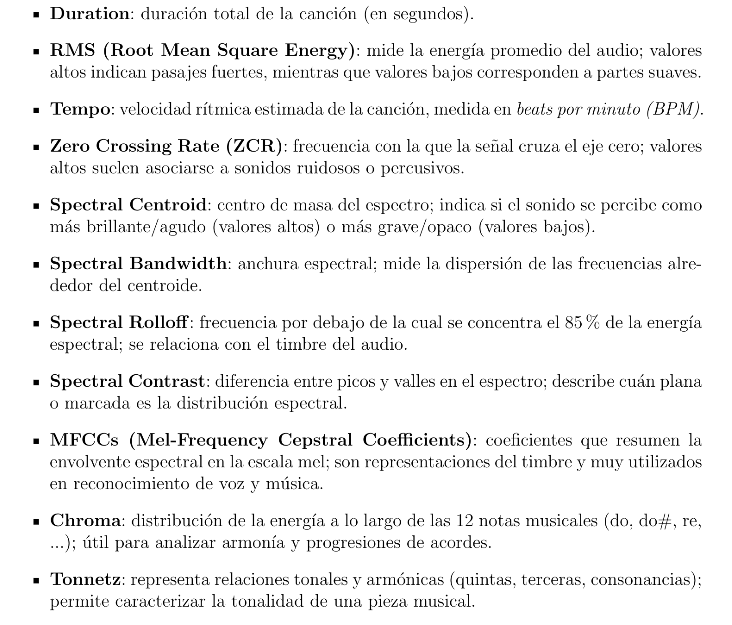
\includegraphics{songs_var_description.png}
\caption{variables}
\end{figure}

    \hypertarget{actividad}{%
\subsection{Actividad}\label{actividad}}

    \begin{figure}
\centering
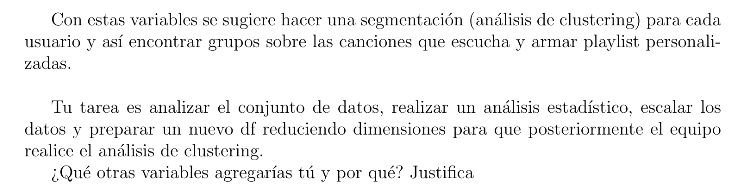
\includegraphics{songs_activity.png}
\caption{actividad}
\end{figure}

    \hypertarget{exploraciuxf3n}{%
\section{Exploración}\label{exploraciuxf3n}}

    \hypertarget{tipo-de-dato-por-variable}{%
\subsubsection{Tipo de dato por
variable}\label{tipo-de-dato-por-variable}}

    \begin{tcolorbox}[breakable, size=fbox, boxrule=1pt, pad at break*=1mm,colback=cellbackground, colframe=cellborder]
\prompt{In}{incolor}{9}{\boxspacing}
\begin{Verbatim}[commandchars=\\\{\}]
\PY{n}{songs1}\PY{o}{.}\PY{n}{info}\PY{p}{(}\PY{p}{)}
\end{Verbatim}
\end{tcolorbox}

    \begin{Verbatim}[commandchars=\\\{\}]
<class 'pandas.core.frame.DataFrame'>
RangeIndex: 175 entries, 0 to 174
Data columns (total 40 columns):
 \#   Column              Non-Null Count  Dtype
---  ------              --------------  -----
 0   archivo             175 non-null    object
 1   duration            175 non-null    float64
 2   rms                 175 non-null    float64
 3   tempo               175 non-null    object
 4   zcr                 175 non-null    float64
 5   spectral\_centroid   175 non-null    float64
 6   spectral\_bandwidth  175 non-null    float64
 7   spectral\_rolloff    175 non-null    float64
 8   spectral\_contrast   175 non-null    float64
 9   mfcc\_1              175 non-null    float64
 10  mfcc\_2              175 non-null    float64
 11  mfcc\_3              175 non-null    float64
 12  mfcc\_4              175 non-null    float64
 13  mfcc\_5              175 non-null    float64
 14  mfcc\_6              175 non-null    float64
 15  mfcc\_7              175 non-null    float64
 16  mfcc\_8              175 non-null    float64
 17  mfcc\_9              175 non-null    float64
 18  mfcc\_10             175 non-null    float64
 19  mfcc\_11             175 non-null    float64
 20  mfcc\_12             175 non-null    float64
 21  mfcc\_13             175 non-null    float64
 22  chroma\_1            175 non-null    float64
 23  chroma\_2            175 non-null    float64
 24  chroma\_3            175 non-null    float64
 25  chroma\_4            175 non-null    float64
 26  chroma\_5            175 non-null    float64
 27  chroma\_6            175 non-null    float64
 28  chroma\_7            175 non-null    float64
 29  chroma\_8            175 non-null    float64
 30  chroma\_9            175 non-null    float64
 31  chroma\_10           175 non-null    float64
 32  chroma\_11           175 non-null    float64
 33  chroma\_12           175 non-null    float64
 34  tonnetz\_1           175 non-null    float64
 35  tonnetz\_2           175 non-null    float64
 36  tonnetz\_3           175 non-null    float64
 37  tonnetz\_4           175 non-null    float64
 38  tonnetz\_5           175 non-null    float64
 39  tonnetz\_6           175 non-null    float64
dtypes: float64(38), object(2)
memory usage: 54.8+ KB
    \end{Verbatim}

    \hypertarget{valores-ausentes}{%
\subsubsection{Valores ausentes}\label{valores-ausentes}}

    \begin{tcolorbox}[breakable, size=fbox, boxrule=1pt, pad at break*=1mm,colback=cellbackground, colframe=cellborder]
\prompt{In}{incolor}{10}{\boxspacing}
\begin{Verbatim}[commandchars=\\\{\}]
\PY{k}{def} \PY{n+nf}{is\PYZus{}na\PYZus{}df}\PY{p}{(}\PY{n}{df}\PY{p}{)}\PY{p}{:}
    \PY{c+c1}{\PYZsh{}Establecemos el resumen de NAs por columna}
    \PY{n}{na\PYZus{}summary} \PY{o}{=} \PY{p}{(}
        \PY{n}{df}\PY{o}{.}\PY{n}{isna}\PY{p}{(}\PY{p}{)}\PY{o}{.}\PY{n}{sum}\PY{p}{(}\PY{p}{)}
        \PY{o}{.}\PY{n}{reset\PYZus{}index}\PY{p}{(}\PY{p}{)}
        \PY{o}{.}\PY{n}{rename}\PY{p}{(}\PY{n}{columns}\PY{o}{=}\PY{p}{\PYZob{}}\PY{l+s+s2}{\PYZdq{}}\PY{l+s+s2}{index}\PY{l+s+s2}{\PYZdq{}}\PY{p}{:} \PY{l+s+s2}{\PYZdq{}}\PY{l+s+s2}{columna}\PY{l+s+s2}{\PYZdq{}}\PY{p}{,} \PY{l+m+mi}{0}\PY{p}{:} \PY{l+s+s2}{\PYZdq{}}\PY{l+s+s2}{n\PYZus{}missing}\PY{l+s+s2}{\PYZdq{}}\PY{p}{\PYZcb{}}\PY{p}{)}
    \PY{p}{)}

    \PY{c+c1}{\PYZsh{}Tomamos totales y prporciones}
    \PY{n}{na\PYZus{}summary}\PY{p}{[}\PY{l+s+s2}{\PYZdq{}}\PY{l+s+s2}{total}\PY{l+s+s2}{\PYZdq{}}\PY{p}{]} \PY{o}{=} \PY{n+nb}{len}\PY{p}{(}\PY{n}{df}\PY{p}{)}
    \PY{n}{na\PYZus{}summary}\PY{p}{[}\PY{l+s+s2}{\PYZdq{}}\PY{l+s+s2}{prop\PYZus{}missing}\PY{l+s+s2}{\PYZdq{}}\PY{p}{]} \PY{o}{=} \PY{n}{na\PYZus{}summary}\PY{p}{[}\PY{l+s+s2}{\PYZdq{}}\PY{l+s+s2}{n\PYZus{}missing}\PY{l+s+s2}{\PYZdq{}}\PY{p}{]} \PY{o}{/} \PY{n}{na\PYZus{}summary}\PY{p}{[}\PY{l+s+s2}{\PYZdq{}}\PY{l+s+s2}{total}\PY{l+s+s2}{\PYZdq{}}\PY{p}{]}
    \PY{n}{na\PYZus{}summary}\PY{p}{[}\PY{l+s+s2}{\PYZdq{}}\PY{l+s+s2}{prop\PYZus{}original}\PY{l+s+s2}{\PYZdq{}}\PY{p}{]} \PY{o}{=} \PY{l+m+mi}{1} \PY{o}{\PYZhy{}} \PY{n}{na\PYZus{}summary}\PY{p}{[}\PY{l+s+s2}{\PYZdq{}}\PY{l+s+s2}{prop\PYZus{}missing}\PY{l+s+s2}{\PYZdq{}}\PY{p}{]}

    \PY{c+c1}{\PYZsh{}Filtramos solo columnas con al menos 1 NA}
    \PY{n}{na\PYZus{}summary} \PY{o}{=} \PY{n}{na\PYZus{}summary}\PY{p}{[}\PY{n}{na\PYZus{}summary}\PY{p}{[}\PY{l+s+s2}{\PYZdq{}}\PY{l+s+s2}{n\PYZus{}missing}\PY{l+s+s2}{\PYZdq{}}\PY{p}{]} \PY{o}{\PYZgt{}} \PY{l+m+mi}{0}\PY{p}{]}\PY{o}{.}\PY{n}{reset\PYZus{}index}\PY{p}{(}\PY{n}{drop}\PY{o}{=}\PY{k+kc}{True}\PY{p}{)}

    \PY{c+c1}{\PYZsh{}Agregamos fila resumen global}
    \PY{n}{total\PYZus{}missing} \PY{o}{=} \PY{n}{df}\PY{o}{.}\PY{n}{isna}\PY{p}{(}\PY{p}{)}\PY{o}{.}\PY{n}{sum}\PY{p}{(}\PY{p}{)}\PY{o}{.}\PY{n}{sum}\PY{p}{(}\PY{p}{)}
    \PY{n}{total\PYZus{}elements} \PY{o}{=} \PY{n}{df}\PY{o}{.}\PY{n}{size}
    \PY{n}{prop\PYZus{}missing\PYZus{}global} \PY{o}{=} \PY{n}{total\PYZus{}missing} \PY{o}{/} \PY{n}{total\PYZus{}elements}
    \PY{n}{prop\PYZus{}original\PYZus{}global} \PY{o}{=} \PY{l+m+mi}{1} \PY{o}{\PYZhy{}} \PY{n}{prop\PYZus{}missing\PYZus{}global}

    \PY{n}{resumen} \PY{o}{=} \PY{n}{pd}\PY{o}{.}\PY{n}{DataFrame}\PY{p}{(}\PY{p}{\PYZob{}}
        \PY{l+s+s2}{\PYZdq{}}\PY{l+s+s2}{columna}\PY{l+s+s2}{\PYZdq{}}\PY{p}{:} \PY{p}{[}\PY{l+s+s2}{\PYZdq{}}\PY{l+s+s2}{TOTAL}\PY{l+s+s2}{\PYZdq{}}\PY{p}{]}\PY{p}{,}
        \PY{l+s+s2}{\PYZdq{}}\PY{l+s+s2}{n\PYZus{}missing}\PY{l+s+s2}{\PYZdq{}}\PY{p}{:} \PY{p}{[}\PY{n}{total\PYZus{}missing}\PY{p}{]}\PY{p}{,}
        \PY{l+s+s2}{\PYZdq{}}\PY{l+s+s2}{total}\PY{l+s+s2}{\PYZdq{}}\PY{p}{:} \PY{p}{[}\PY{n}{total\PYZus{}elements}\PY{p}{]}\PY{p}{,}
        \PY{l+s+s2}{\PYZdq{}}\PY{l+s+s2}{prop\PYZus{}missing}\PY{l+s+s2}{\PYZdq{}}\PY{p}{:} \PY{p}{[}\PY{n}{prop\PYZus{}missing\PYZus{}global}\PY{p}{]}\PY{p}{,}
        \PY{l+s+s2}{\PYZdq{}}\PY{l+s+s2}{prop\PYZus{}original}\PY{l+s+s2}{\PYZdq{}}\PY{p}{:} \PY{p}{[}\PY{n}{prop\PYZus{}original\PYZus{}global}\PY{p}{]}
    \PY{p}{\PYZcb{}}\PY{p}{)}

    \PY{c+c1}{\PYZsh{}Creamos la tabla}
    \PY{n}{na\PYZus{}summary} \PY{o}{=} \PY{n}{pd}\PY{o}{.}\PY{n}{concat}\PY{p}{(}\PY{p}{[}\PY{n}{na\PYZus{}summary}\PY{p}{,} \PY{n}{resumen}\PY{p}{]}\PY{p}{,} \PY{n}{ignore\PYZus{}index}\PY{o}{=}\PY{k+kc}{True}\PY{p}{)}

    \PY{k}{return} \PY{n}{na\PYZus{}summary}
\end{Verbatim}
\end{tcolorbox}

    \begin{tcolorbox}[breakable, size=fbox, boxrule=1pt, pad at break*=1mm,colback=cellbackground, colframe=cellborder]
\prompt{In}{incolor}{11}{\boxspacing}
\begin{Verbatim}[commandchars=\\\{\}]
\PY{n}{is\PYZus{}na\PYZus{}df}\PY{p}{(}\PY{n}{songs1}\PY{p}{)}
\end{Verbatim}
\end{tcolorbox}

            \begin{tcolorbox}[breakable, size=fbox, boxrule=.5pt, pad at break*=1mm, opacityfill=0]
\prompt{Out}{outcolor}{11}{\boxspacing}
\begin{Verbatim}[commandchars=\\\{\}]
  columna  n\_missing  total  prop\_missing  prop\_original
0   TOTAL          0   7000           0.0            1.0
\end{Verbatim}
\end{tcolorbox}
        
    No hay valores ausentes por lo que no hace falta aplicar un método de
imputación.

    \hypertarget{distribuciuxf3n-de-variables-numuxe9ricas}{%
\subsubsection{Distribución de variables
numéricas}\label{distribuciuxf3n-de-variables-numuxe9ricas}}

    \begin{tcolorbox}[breakable, size=fbox, boxrule=1pt, pad at break*=1mm,colback=cellbackground, colframe=cellborder]
\prompt{In}{incolor}{12}{\boxspacing}
\begin{Verbatim}[commandchars=\\\{\}]
\PY{n}{var\PYZus{}cat} \PY{o}{=} \PY{n}{songs1}\PY{o}{.}\PY{n}{select\PYZus{}dtypes}\PY{p}{(}\PY{p}{[}\PY{l+s+s1}{\PYZsq{}}\PY{l+s+s1}{object}\PY{l+s+s1}{\PYZsq{}}\PY{p}{]}\PY{p}{)}\PY{o}{.}\PY{n}{columns}\PY{o}{.}\PY{n}{tolist}\PY{p}{(}\PY{p}{)}
\PY{n}{var\PYZus{}cat}
\end{Verbatim}
\end{tcolorbox}

            \begin{tcolorbox}[breakable, size=fbox, boxrule=.5pt, pad at break*=1mm, opacityfill=0]
\prompt{Out}{outcolor}{12}{\boxspacing}
\begin{Verbatim}[commandchars=\\\{\}]
['archivo', 'tempo']
\end{Verbatim}
\end{tcolorbox}
        
    \begin{tcolorbox}[breakable, size=fbox, boxrule=1pt, pad at break*=1mm,colback=cellbackground, colframe=cellborder]
\prompt{In}{incolor}{13}{\boxspacing}
\begin{Verbatim}[commandchars=\\\{\}]
\PY{n}{songs1}\PY{p}{[}\PY{l+s+s1}{\PYZsq{}}\PY{l+s+s1}{tempo\PYZus{}num}\PY{l+s+s1}{\PYZsq{}}\PY{p}{]} \PY{o}{=} \PY{n}{songs1}\PY{p}{[}\PY{l+s+s1}{\PYZsq{}}\PY{l+s+s1}{tempo}\PY{l+s+s1}{\PYZsq{}}\PY{p}{]}\PY{o}{.}\PY{n}{str}\PY{p}{[}\PY{l+m+mi}{1}\PY{p}{:}\PY{o}{\PYZhy{}}\PY{l+m+mi}{1}\PY{p}{]}\PY{o}{.}\PY{n}{astype}\PY{p}{(}\PY{n+nb}{float}\PY{p}{)}
\end{Verbatim}
\end{tcolorbox}

    \begin{tcolorbox}[breakable, size=fbox, boxrule=1pt, pad at break*=1mm,colback=cellbackground, colframe=cellborder]
\prompt{In}{incolor}{14}{\boxspacing}
\begin{Verbatim}[commandchars=\\\{\}]
\PY{k}{def} \PY{n+nf}{guess\PYZus{}lang\PYZus{}heuristic}\PY{p}{(}\PY{n}{text}\PY{p}{:} \PY{n+nb}{str}\PY{p}{)}\PY{p}{:}

    \PY{n}{spanish\PYZus{}words} \PY{o}{=} \PY{p}{\PYZob{}}
        \PY{l+s+s2}{\PYZdq{}}\PY{l+s+s2}{el}\PY{l+s+s2}{\PYZdq{}}\PY{p}{,}\PY{l+s+s2}{\PYZdq{}}\PY{l+s+s2}{la}\PY{l+s+s2}{\PYZdq{}}\PY{p}{,}\PY{l+s+s2}{\PYZdq{}}\PY{l+s+s2}{los}\PY{l+s+s2}{\PYZdq{}}\PY{p}{,}\PY{l+s+s2}{\PYZdq{}}\PY{l+s+s2}{las}\PY{l+s+s2}{\PYZdq{}}\PY{p}{,}\PY{l+s+s2}{\PYZdq{}}\PY{l+s+s2}{un}\PY{l+s+s2}{\PYZdq{}}\PY{p}{,}\PY{l+s+s2}{\PYZdq{}}\PY{l+s+s2}{una}\PY{l+s+s2}{\PYZdq{}}\PY{p}{,}\PY{l+s+s2}{\PYZdq{}}\PY{l+s+s2}{unos}\PY{l+s+s2}{\PYZdq{}}\PY{p}{,}\PY{l+s+s2}{\PYZdq{}}\PY{l+s+s2}{unas}\PY{l+s+s2}{\PYZdq{}}\PY{p}{,}\PY{l+s+s2}{\PYZdq{}}\PY{l+s+s2}{de}\PY{l+s+s2}{\PYZdq{}}\PY{p}{,}\PY{l+s+s2}{\PYZdq{}}\PY{l+s+s2}{del}\PY{l+s+s2}{\PYZdq{}}\PY{p}{,}\PY{l+s+s2}{\PYZdq{}}\PY{l+s+s2}{al}\PY{l+s+s2}{\PYZdq{}}\PY{p}{,}\PY{l+s+s2}{\PYZdq{}}\PY{l+s+s2}{y}\PY{l+s+s2}{\PYZdq{}}\PY{p}{,}\PY{l+s+s2}{\PYZdq{}}\PY{l+s+s2}{o}\PY{l+s+s2}{\PYZdq{}}\PY{p}{,}\PY{l+s+s2}{\PYZdq{}}\PY{l+s+s2}{u}\PY{l+s+s2}{\PYZdq{}}\PY{p}{,}
        \PY{l+s+s2}{\PYZdq{}}\PY{l+s+s2}{que}\PY{l+s+s2}{\PYZdq{}}\PY{p}{,}\PY{l+s+s2}{\PYZdq{}}\PY{l+s+s2}{como}\PY{l+s+s2}{\PYZdq{}}\PY{p}{,}\PY{l+s+s2}{\PYZdq{}}\PY{l+s+s2}{con}\PY{l+s+s2}{\PYZdq{}}\PY{p}{,}\PY{l+s+s2}{\PYZdq{}}\PY{l+s+s2}{por}\PY{l+s+s2}{\PYZdq{}}\PY{p}{,}\PY{l+s+s2}{\PYZdq{}}\PY{l+s+s2}{para}\PY{l+s+s2}{\PYZdq{}}\PY{p}{,}\PY{l+s+s2}{\PYZdq{}}\PY{l+s+s2}{sin}\PY{l+s+s2}{\PYZdq{}}\PY{p}{,}\PY{l+s+s2}{\PYZdq{}}\PY{l+s+s2}{sobre}\PY{l+s+s2}{\PYZdq{}}\PY{p}{,}\PY{l+s+s2}{\PYZdq{}}\PY{l+s+s2}{entre}\PY{l+s+s2}{\PYZdq{}}\PY{p}{,}\PY{l+s+s2}{\PYZdq{}}\PY{l+s+s2}{más}\PY{l+s+s2}{\PYZdq{}}\PY{p}{,}\PY{l+s+s2}{\PYZdq{}}\PY{l+s+s2}{menos}\PY{l+s+s2}{\PYZdq{}}\PY{p}{,}\PY{l+s+s2}{\PYZdq{}}\PY{l+s+s2}{mi}\PY{l+s+s2}{\PYZdq{}}\PY{p}{,}\PY{l+s+s2}{\PYZdq{}}\PY{l+s+s2}{tu}\PY{l+s+s2}{\PYZdq{}}\PY{p}{,}
        \PY{l+s+s2}{\PYZdq{}}\PY{l+s+s2}{te}\PY{l+s+s2}{\PYZdq{}}\PY{p}{,}\PY{l+s+s2}{\PYZdq{}}\PY{l+s+s2}{se}\PY{l+s+s2}{\PYZdq{}}\PY{p}{,}\PY{l+s+s2}{\PYZdq{}}\PY{l+s+s2}{me}\PY{l+s+s2}{\PYZdq{}}\PY{p}{,}\PY{l+s+s2}{\PYZdq{}}\PY{l+s+s2}{lo}\PY{l+s+s2}{\PYZdq{}}\PY{p}{,}\PY{l+s+s2}{\PYZdq{}}\PY{l+s+s2}{le}\PY{l+s+s2}{\PYZdq{}}\PY{p}{,}\PY{l+s+s2}{\PYZdq{}}\PY{l+s+s2}{su}\PY{l+s+s2}{\PYZdq{}}\PY{p}{,}\PY{l+s+s2}{\PYZdq{}}\PY{l+s+s2}{si}\PY{l+s+s2}{\PYZdq{}}\PY{p}{,}\PY{l+s+s2}{\PYZdq{}}\PY{l+s+s2}{ya}\PY{l+s+s2}{\PYZdq{}}\PY{p}{,}\PY{l+s+s2}{\PYZdq{}}\PY{l+s+s2}{no}\PY{l+s+s2}{\PYZdq{}}\PY{p}{,}\PY{l+s+s2}{\PYZdq{}}\PY{l+s+s2}{sí}\PY{l+s+s2}{\PYZdq{}}\PY{p}{,}\PY{l+s+s2}{\PYZdq{}}\PY{l+s+s2}{a}\PY{l+s+s2}{\PYZdq{}}\PY{p}{,}\PY{l+s+s2}{\PYZdq{}}\PY{l+s+s2}{en}\PY{l+s+s2}{\PYZdq{}}
    \PY{p}{\PYZcb{}}

    \PY{n}{tokens} \PY{o}{=} \PY{p}{\PYZob{}}\PY{n}{t} \PY{k}{for} \PY{n}{t} \PY{o+ow}{in} \PY{n}{re}\PY{o}{.}\PY{n}{findall}\PY{p}{(}\PY{l+s+sa}{r}\PY{l+s+s2}{\PYZdq{}}\PY{l+s+s2}{\PYZbs{}}\PY{l+s+s2}{b}\PY{l+s+s2}{\PYZbs{}}\PY{l+s+s2}{w+}\PY{l+s+s2}{\PYZbs{}}\PY{l+s+s2}{b}\PY{l+s+s2}{\PYZdq{}}\PY{p}{,} \PY{n}{text}\PY{p}{)}\PY{p}{\PYZcb{}}
    \PY{n}{hits} \PY{o}{=} \PY{n+nb}{len}\PY{p}{(}\PY{n}{tokens} \PY{o}{\PYZam{}} \PY{n}{spanish\PYZus{}words}\PY{p}{)}
    
    \PY{c+c1}{\PYZsh{} si tiene acentos/símbolos muy comunes en español, suma}
    \PY{n}{accent\PYZus{}bonus} \PY{o}{=} \PY{l+m+mi}{1} \PY{k}{if} \PY{n}{re}\PY{o}{.}\PY{n}{search}\PY{p}{(}\PY{l+s+sa}{r}\PY{l+s+s2}{\PYZdq{}}\PY{l+s+s2}{[áéíóúñü]}\PY{l+s+s2}{\PYZdq{}}\PY{p}{,} \PY{n}{text}\PY{o}{.}\PY{n}{lower}\PY{p}{(}\PY{p}{)}\PY{p}{)} \PY{k}{else} \PY{l+m+mi}{0}
    \PY{n}{score\PYZus{}es} \PY{o}{=} \PY{n}{hits} \PY{o}{+} \PY{n}{accent\PYZus{}bonus}
    
    \PY{c+c1}{\PYZsh{} título muy corto =\PYZgt{} baja confianza}
    \PY{n}{conf} \PY{o}{=} \PY{n+nb}{min}\PY{p}{(}\PY{l+m+mf}{1.0}\PY{p}{,} \PY{l+m+mf}{0.2}\PY{o}{*}\PY{n}{score\PYZus{}es} \PY{o}{+} \PY{l+m+mf}{0.2}\PY{o}{*}\PY{p}{(}\PY{n+nb}{len}\PY{p}{(}\PY{n}{tokens}\PY{p}{)} \PY{o}{\PYZgt{}}\PY{o}{=} \PY{l+m+mi}{3}\PY{p}{)}\PY{p}{)}
    \PY{k}{if} \PY{n}{score\PYZus{}es} \PY{o}{\PYZgt{}}\PY{o}{=} \PY{l+m+mi}{2}\PY{p}{:}
        \PY{k}{return} \PY{l+s+s2}{\PYZdq{}}\PY{l+s+s2}{es}\PY{l+s+s2}{\PYZdq{}}\PY{p}{,} \PY{n}{conf}

    \PY{c+c1}{\PYZsh{} si no hay indicios en español y tiene muchas palabras comunes en inglés}
    \PY{n}{english\PYZus{}words} \PY{o}{=} \PY{p}{\PYZob{}}\PY{l+s+s2}{\PYZdq{}}\PY{l+s+s2}{the}\PY{l+s+s2}{\PYZdq{}}\PY{p}{,}\PY{l+s+s2}{\PYZdq{}}\PY{l+s+s2}{and}\PY{l+s+s2}{\PYZdq{}}\PY{p}{,}\PY{l+s+s2}{\PYZdq{}}\PY{l+s+s2}{you}\PY{l+s+s2}{\PYZdq{}}\PY{p}{,}\PY{l+s+s2}{\PYZdq{}}\PY{l+s+s2}{your}\PY{l+s+s2}{\PYZdq{}}\PY{p}{,}\PY{l+s+s2}{\PYZdq{}}\PY{l+s+s2}{i}\PY{l+s+s2}{\PYZdq{}}\PY{p}{,}\PY{l+s+s2}{\PYZdq{}}\PY{l+s+s2}{me}\PY{l+s+s2}{\PYZdq{}}\PY{p}{,}\PY{l+s+s2}{\PYZdq{}}\PY{l+s+s2}{my}\PY{l+s+s2}{\PYZdq{}}\PY{p}{,}\PY{l+s+s2}{\PYZdq{}}\PY{l+s+s2}{on}\PY{l+s+s2}{\PYZdq{}}\PY{p}{,}\PY{l+s+s2}{\PYZdq{}}\PY{l+s+s2}{in}\PY{l+s+s2}{\PYZdq{}}\PY{p}{,}\PY{l+s+s2}{\PYZdq{}}\PY{l+s+s2}{with}\PY{l+s+s2}{\PYZdq{}}\PY{p}{,}\PY{l+s+s2}{\PYZdq{}}\PY{l+s+s2}{for}\PY{l+s+s2}{\PYZdq{}}\PY{p}{,}\PY{l+s+s2}{\PYZdq{}}\PY{l+s+s2}{of}\PY{l+s+s2}{\PYZdq{}}\PY{p}{,}\PY{l+s+s2}{\PYZdq{}}\PY{l+s+s2}{to}\PY{l+s+s2}{\PYZdq{}}\PY{p}{,}\PY{l+s+s2}{\PYZdq{}}\PY{l+s+s2}{from}\PY{l+s+s2}{\PYZdq{}}\PY{p}{,}\PY{l+s+s2}{\PYZdq{}}\PY{l+s+s2}{at}\PY{l+s+s2}{\PYZdq{}}\PY{p}{,}\PY{l+s+s2}{\PYZdq{}}\PY{l+s+s2}{it}\PY{l+s+s2}{\PYZdq{}}\PY{p}{,}\PY{l+s+s2}{\PYZdq{}}\PY{l+s+s2}{is}\PY{l+s+s2}{\PYZdq{}}\PY{p}{\PYZcb{}}
    \PY{n}{hits\PYZus{}en} \PY{o}{=} \PY{n+nb}{len}\PY{p}{(}\PY{n}{tokens} \PY{o}{\PYZam{}} \PY{n}{english\PYZus{}words}\PY{p}{)}
    \PY{k}{if} \PY{n}{hits\PYZus{}en} \PY{o}{\PYZgt{}}\PY{o}{=} \PY{l+m+mi}{2}\PY{p}{:}
        \PY{k}{return} \PY{l+s+s2}{\PYZdq{}}\PY{l+s+s2}{en}\PY{l+s+s2}{\PYZdq{}}\PY{p}{,} \PY{n+nb}{max}\PY{p}{(}\PY{n}{conf}\PY{p}{,} \PY{l+m+mf}{0.6}\PY{p}{)}
        
    \PY{c+c1}{\PYZsh{} por defecto “en” si todo está en ASCII y sin acentos; si no, desconocido}
    \PY{k}{return} \PY{p}{(}\PY{l+s+s2}{\PYZdq{}}\PY{l+s+s2}{en}\PY{l+s+s2}{\PYZdq{}}\PY{p}{,} \PY{l+m+mf}{0.5}\PY{p}{)} \PY{k}{if} \PY{n}{text}\PY{o}{.}\PY{n}{isascii}\PY{p}{(}\PY{p}{)} \PY{k}{else} \PY{p}{(}\PY{l+s+s2}{\PYZdq{}}\PY{l+s+s2}{unk}\PY{l+s+s2}{\PYZdq{}}\PY{p}{,} \PY{l+m+mf}{0.3}\PY{p}{)}
\end{Verbatim}
\end{tcolorbox}

    \begin{tcolorbox}[breakable, size=fbox, boxrule=1pt, pad at break*=1mm,colback=cellbackground, colframe=cellborder]
\prompt{In}{incolor}{15}{\boxspacing}
\begin{Verbatim}[commandchars=\\\{\}]
\PY{k}{def} \PY{n+nf}{label\PYZus{}from\PYZus{}code}\PY{p}{(}\PY{n}{code}\PY{p}{)}\PY{p}{:}
    \PY{k}{return} \PY{p}{\PYZob{}}\PY{l+s+s2}{\PYZdq{}}\PY{l+s+s2}{es}\PY{l+s+s2}{\PYZdq{}}\PY{p}{:}\PY{l+s+s2}{\PYZdq{}}\PY{l+s+s2}{Español}\PY{l+s+s2}{\PYZdq{}}\PY{p}{,}\PY{l+s+s2}{\PYZdq{}}\PY{l+s+s2}{en}\PY{l+s+s2}{\PYZdq{}}\PY{p}{:}\PY{l+s+s2}{\PYZdq{}}\PY{l+s+s2}{Inglés}\PY{l+s+s2}{\PYZdq{}}\PY{p}{,}\PY{l+s+s2}{\PYZdq{}}\PY{l+s+s2}{unk}\PY{l+s+s2}{\PYZdq{}}\PY{p}{:}\PY{l+s+s2}{\PYZdq{}}\PY{l+s+s2}{Desconocido}\PY{l+s+s2}{\PYZdq{}}\PY{p}{\PYZcb{}}\PY{o}{.}\PY{n}{get}\PY{p}{(}\PY{n}{code}\PY{p}{,}\PY{l+s+s2}{\PYZdq{}}\PY{l+s+s2}{Desconocido}\PY{l+s+s2}{\PYZdq{}}\PY{p}{)}
\end{Verbatim}
\end{tcolorbox}

    \begin{tcolorbox}[breakable, size=fbox, boxrule=1pt, pad at break*=1mm,colback=cellbackground, colframe=cellborder]
\prompt{In}{incolor}{16}{\boxspacing}
\begin{Verbatim}[commandchars=\\\{\}]
\PY{n}{songs1}\PY{p}{[}\PY{l+s+s1}{\PYZsq{}}\PY{l+s+s1}{archivo}\PY{l+s+s1}{\PYZsq{}}\PY{p}{]} \PY{o}{=} \PY{n}{songs1}\PY{p}{[}\PY{l+s+s1}{\PYZsq{}}\PY{l+s+s1}{archivo}\PY{l+s+s1}{\PYZsq{}}\PY{p}{]}\PY{o}{.}\PY{n}{str}\PY{o}{.}\PY{n}{replace}\PY{p}{(}\PY{l+s+s1}{\PYZsq{}}\PY{l+s+s1}{.mp3}\PY{l+s+s1}{\PYZsq{}} \PY{p}{,} \PY{l+s+s1}{\PYZsq{}}\PY{l+s+s1}{\PYZsq{}}\PY{p}{)}\PY{o}{.}\PY{n}{str}\PY{o}{.}\PY{n}{lower}\PY{p}{(}\PY{p}{)}
\end{Verbatim}
\end{tcolorbox}

    \begin{tcolorbox}[breakable, size=fbox, boxrule=1pt, pad at break*=1mm,colback=cellbackground, colframe=cellborder]
\prompt{In}{incolor}{17}{\boxspacing}
\begin{Verbatim}[commandchars=\\\{\}]
\PY{n}{songs1}\PY{p}{[}\PY{l+s+s1}{\PYZsq{}}\PY{l+s+s1}{archivo}\PY{l+s+s1}{\PYZsq{}}\PY{p}{]}\PY{o}{.}\PY{n}{to\PYZus{}csv}\PY{p}{(}\PY{l+s+s1}{\PYZsq{}}\PY{l+s+s1}{canciones.csv}\PY{l+s+s1}{\PYZsq{}}\PY{p}{)}
\end{Verbatim}
\end{tcolorbox}

    \begin{tcolorbox}[breakable, size=fbox, boxrule=1pt, pad at break*=1mm,colback=cellbackground, colframe=cellborder]
\prompt{In}{incolor}{18}{\boxspacing}
\begin{Verbatim}[commandchars=\\\{\}]
\PY{n}{songs1}\PY{p}{[}\PY{l+s+s2}{\PYZdq{}}\PY{l+s+s2}{lang\PYZus{}code}\PY{l+s+s2}{\PYZdq{}}\PY{p}{]}\PY{p}{,} \PY{n}{songs1}\PY{p}{[}\PY{l+s+s2}{\PYZdq{}}\PY{l+s+s2}{lang\PYZus{}conf}\PY{l+s+s2}{\PYZdq{}}\PY{p}{]} \PY{o}{=} \PY{n+nb}{zip}\PY{p}{(}\PY{o}{*}\PY{n}{songs1}\PY{p}{[}\PY{l+s+s2}{\PYZdq{}}\PY{l+s+s2}{archivo}\PY{l+s+s2}{\PYZdq{}}\PY{p}{]}\PY{o}{.}\PY{n}{map}\PY{p}{(}\PY{n}{guess\PYZus{}lang\PYZus{}heuristic}\PY{p}{)}\PY{p}{)}
\PY{n}{songs1}\PY{p}{[}\PY{l+s+s2}{\PYZdq{}}\PY{l+s+s2}{lang}\PY{l+s+s2}{\PYZdq{}}\PY{p}{]} \PY{o}{=} \PY{n}{songs1}\PY{p}{[}\PY{l+s+s2}{\PYZdq{}}\PY{l+s+s2}{lang\PYZus{}code}\PY{l+s+s2}{\PYZdq{}}\PY{p}{]}\PY{o}{.}\PY{n}{map}\PY{p}{(}\PY{n}{label\PYZus{}from\PYZus{}code}\PY{p}{)}
\end{Verbatim}
\end{tcolorbox}

    \begin{tcolorbox}[breakable, size=fbox, boxrule=1pt, pad at break*=1mm,colback=cellbackground, colframe=cellborder]
\prompt{In}{incolor}{19}{\boxspacing}
\begin{Verbatim}[commandchars=\\\{\}]
\PY{n}{songs1}\PY{o}{.}\PY{n}{head}\PY{p}{(}\PY{l+m+mi}{3}\PY{p}{)}
\end{Verbatim}
\end{tcolorbox}

            \begin{tcolorbox}[breakable, size=fbox, boxrule=.5pt, pad at break*=1mm, opacityfill=0]
\prompt{Out}{outcolor}{19}{\boxspacing}
\begin{Verbatim}[commandchars=\\\{\}]
                archivo    duration       rms           tempo       zcr  \textbackslash{}
0             02 maroon  218.305306  0.269286  [107.66601562]  0.030423
1          03 anti-hero  200.724898  0.251603   [97.50884434]  0.042470
2  04 snow on the beach  256.156735  0.191276  [109.95678191]  0.026679

   spectral\_centroid  spectral\_bandwidth  spectral\_rolloff  spectral\_contrast  \textbackslash{}
0        2131.429071         3054.294473       4833.956751          21.985519
1        2270.523020         2887.932364       4680.853820          20.961313
2        1691.923217         2516.562246       3338.831279          21.885129

      mfcc\_1  {\ldots}  tonnetz\_1  tonnetz\_2  tonnetz\_3  tonnetz\_4  tonnetz\_5  \textbackslash{}
0 -165.31206  {\ldots}   0.275898   0.210128   0.175254   0.011638   0.049738
1 -116.05038  {\ldots}   0.067301  -0.201125  -0.039244   0.056137   0.023695
2 -205.33786  {\ldots}   0.140940  -0.188128  -0.098086  -0.042389   0.013691

   tonnetz\_6   tempo\_num  lang\_code  lang\_conf    lang
0  -0.057944  107.666016         en        0.5  Inglés
1  -0.028362   97.508844         en        0.5  Inglés
2  -0.021691  109.956782         en        0.6  Inglés

[3 rows x 44 columns]
\end{Verbatim}
\end{tcolorbox}
        
    \begin{tcolorbox}[breakable, size=fbox, boxrule=1pt, pad at break*=1mm,colback=cellbackground, colframe=cellborder]
\prompt{In}{incolor}{20}{\boxspacing}
\begin{Verbatim}[commandchars=\\\{\}]
\PY{k}{class} \PY{n+nc}{analyze}\PY{p}{:}
    \PY{c+c1}{\PYZsh{} Inicializamos la clase}
    \PY{k}{def} \PY{n+nf+fm}{\PYZus{}\PYZus{}init\PYZus{}\PYZus{}}\PY{p}{(}\PY{n+nb+bp}{self}\PY{p}{,} \PY{n}{df}\PY{p}{,} \PY{n}{num\PYZus{}vars}\PY{p}{,} \PY{n}{cat\PYZus{}vars}\PY{p}{)}\PY{p}{:}
        \PY{n+nb+bp}{self}\PY{o}{.}\PY{n}{df} \PY{o}{=} \PY{n}{df}
        \PY{n+nb+bp}{self}\PY{o}{.}\PY{n}{num\PYZus{}vars} \PY{o}{=} \PY{n}{num\PYZus{}vars}
        \PY{n+nb+bp}{self}\PY{o}{.}\PY{n}{cat\PYZus{}vars} \PY{o}{=} \PY{n}{cat\PYZus{}vars}

    \PY{c+c1}{\PYZsh{}Método para graficar variables numéricas (cada una en figura independiente)}
    \PY{k}{def} \PY{n+nf}{plot\PYZus{}num}\PY{p}{(}\PY{n+nb+bp}{self}\PY{p}{)}\PY{p}{:}
        \PY{k}{for} \PY{n}{var} \PY{o+ow}{in} \PY{n+nb+bp}{self}\PY{o}{.}\PY{n}{num\PYZus{}vars}\PY{p}{:}
            \PY{n}{fig} \PY{o}{=} \PY{n}{make\PYZus{}subplots}\PY{p}{(}\PY{n}{rows}\PY{o}{=}\PY{l+m+mi}{1}\PY{p}{,} \PY{n}{cols}\PY{o}{=}\PY{l+m+mi}{2}\PY{p}{,} \PY{n}{subplot\PYZus{}titles}\PY{o}{=}\PY{p}{(}\PY{l+s+sa}{f}\PY{l+s+s2}{\PYZdq{}}\PY{l+s+si}{\PYZob{}}\PY{n}{var}\PY{l+s+si}{\PYZcb{}}\PY{l+s+s2}{ \PYZhy{} Boxplot}\PY{l+s+s2}{\PYZdq{}}\PY{p}{,} \PY{l+s+sa}{f}\PY{l+s+s2}{\PYZdq{}}\PY{l+s+si}{\PYZob{}}\PY{n}{var}\PY{l+s+si}{\PYZcb{}}\PY{l+s+s2}{ \PYZhy{} Histograma}\PY{l+s+s2}{\PYZdq{}}\PY{p}{)}\PY{p}{)}

            \PY{c+c1}{\PYZsh{} Boxplot}
            \PY{n}{fig}\PY{o}{.}\PY{n}{add\PYZus{}trace}\PY{p}{(}
                \PY{n}{go}\PY{o}{.}\PY{n}{Box}\PY{p}{(}\PY{n}{y}\PY{o}{=}\PY{n+nb+bp}{self}\PY{o}{.}\PY{n}{df}\PY{p}{[}\PY{n}{var}\PY{p}{]}\PY{p}{,} \PY{n}{name}\PY{o}{=}\PY{l+s+s2}{\PYZdq{}}\PY{l+s+s2}{Boxplot}\PY{l+s+s2}{\PYZdq{}}\PY{p}{,} \PY{n}{marker\PYZus{}color}\PY{o}{=}\PY{l+s+s2}{\PYZdq{}}\PY{l+s+s2}{\PYZsh{}008080}\PY{l+s+s2}{\PYZdq{}}\PY{p}{)}\PY{p}{,}
                \PY{n}{row}\PY{o}{=}\PY{l+m+mi}{1}\PY{p}{,} \PY{n}{col}\PY{o}{=}\PY{l+m+mi}{1}
            \PY{p}{)}

            \PY{c+c1}{\PYZsh{} Histograma}
            \PY{n}{fig}\PY{o}{.}\PY{n}{add\PYZus{}trace}\PY{p}{(}
                \PY{n}{go}\PY{o}{.}\PY{n}{Histogram}\PY{p}{(}\PY{n}{x}\PY{o}{=}\PY{n+nb+bp}{self}\PY{o}{.}\PY{n}{df}\PY{p}{[}\PY{n}{var}\PY{p}{]}\PY{p}{,} \PY{n}{name}\PY{o}{=}\PY{l+s+s2}{\PYZdq{}}\PY{l+s+s2}{Histograma}\PY{l+s+s2}{\PYZdq{}}\PY{p}{,}
                             \PY{c+c1}{\PYZsh{}marker\PYZus{}color=\PYZdq{}\PYZsh{}00a77d\PYZdq{}, }
                             \PY{c+c1}{\PYZsh{}marker\PYZus{}color=\PYZsq{}\PYZsh{}722F37\PYZsq{},}
                             \PY{n}{marker\PYZus{}color}\PY{o}{=}\PY{l+s+s2}{\PYZdq{}}\PY{l+s+s2}{rgba(114, 47, 55, 0.5)}\PY{l+s+s2}{\PYZdq{}}\PY{p}{,}  \PY{c+c1}{\PYZsh{} burdeos con 50\PYZpc{} transparencia}
                             \PY{n}{nbinsx}\PY{o}{=}\PY{l+m+mi}{50}\PY{p}{,}
                             \PY{n}{histnorm}\PY{o}{=}\PY{l+s+s1}{\PYZsq{}}\PY{l+s+s1}{probability density}\PY{l+s+s1}{\PYZsq{}}\PY{p}{)}\PY{p}{,}
                \PY{n}{row}\PY{o}{=}\PY{l+m+mi}{1}\PY{p}{,} \PY{n}{col}\PY{o}{=}\PY{l+m+mi}{2}
            \PY{p}{)}

            \PY{n}{fig}\PY{o}{.}\PY{n}{update\PYZus{}layout}\PY{p}{(}\PY{n}{title\PYZus{}text}\PY{o}{=}\PY{l+s+sa}{f}\PY{l+s+s2}{\PYZdq{}}\PY{l+s+s2}{Variable numérica: }\PY{l+s+si}{\PYZob{}}\PY{n}{var}\PY{l+s+si}{\PYZcb{}}\PY{l+s+s2}{\PYZdq{}}\PY{p}{,} \PY{n}{height}\PY{o}{=}\PY{l+m+mi}{400}\PY{p}{,} \PY{n}{width}\PY{o}{=}\PY{l+m+mi}{800}\PY{p}{)}
            \PY{n}{fig}\PY{o}{.}\PY{n}{show}\PY{p}{(}\PY{p}{)}

    \PY{c+c1}{\PYZsh{}Método para graficar variables categóricas}
    \PY{k}{def} \PY{n+nf}{plot\PYZus{}cat}\PY{p}{(}\PY{n+nb+bp}{self}\PY{p}{)}\PY{p}{:}
        \PY{n}{n} \PY{o}{=} \PY{n+nb}{len}\PY{p}{(}\PY{n+nb+bp}{self}\PY{o}{.}\PY{n}{cat\PYZus{}vars}\PY{p}{)}
        \PY{n}{cols} \PY{o}{=} \PY{l+m+mi}{2}
        \PY{n}{rows} \PY{o}{=} \PY{p}{(}\PY{n}{n} \PY{o}{+} \PY{l+m+mi}{1}\PY{p}{)} \PY{o}{/}\PY{o}{/} \PY{n}{cols} \PY{k}{if} \PY{n}{n} \PY{o}{\PYZgt{}} \PY{l+m+mi}{1} \PY{k}{else} \PY{l+m+mi}{1}

        \PY{n}{fig} \PY{o}{=} \PY{n}{make\PYZus{}subplots}\PY{p}{(}
            \PY{n}{rows}\PY{o}{=}\PY{n}{rows}\PY{p}{,} \PY{n}{cols}\PY{o}{=}\PY{n}{cols}\PY{p}{,}
            \PY{n}{specs}\PY{o}{=}\PY{p}{[}\PY{p}{[}\PY{p}{\PYZob{}}\PY{l+s+s1}{\PYZsq{}}\PY{l+s+s1}{type}\PY{l+s+s1}{\PYZsq{}}\PY{p}{:}\PY{l+s+s1}{\PYZsq{}}\PY{l+s+s1}{domain}\PY{l+s+s1}{\PYZsq{}}\PY{p}{\PYZcb{}}\PY{p}{]}\PY{o}{*}\PY{n}{cols} \PY{k}{for} \PY{n}{\PYZus{}} \PY{o+ow}{in} \PY{n+nb}{range}\PY{p}{(}\PY{n}{rows}\PY{p}{)}\PY{p}{]}\PY{p}{,}
            \PY{n}{subplot\PYZus{}titles}\PY{o}{=}\PY{n+nb+bp}{self}\PY{o}{.}\PY{n}{cat\PYZus{}vars}
        \PY{p}{)}

        \PY{k}{for} \PY{n}{i}\PY{p}{,} \PY{n}{var} \PY{o+ow}{in} \PY{n+nb}{enumerate}\PY{p}{(}\PY{n+nb+bp}{self}\PY{o}{.}\PY{n}{cat\PYZus{}vars}\PY{p}{)}\PY{p}{:}
            \PY{n}{row} \PY{o}{=} \PY{n}{i} \PY{o}{/}\PY{o}{/} \PY{n}{cols} \PY{o}{+} \PY{l+m+mi}{1}
            \PY{n}{col} \PY{o}{=} \PY{n}{i} \PY{o}{\PYZpc{}} \PY{n}{cols} \PY{o}{+} \PY{l+m+mi}{1}

            \PY{n}{value\PYZus{}counts} \PY{o}{=} \PY{n+nb+bp}{self}\PY{o}{.}\PY{n}{df}\PY{p}{[}\PY{n}{var}\PY{p}{]}\PY{o}{.}\PY{n}{value\PYZus{}counts}\PY{p}{(}\PY{p}{)}
            \PY{n}{labels} \PY{o}{=} \PY{n}{value\PYZus{}counts}\PY{o}{.}\PY{n}{index}\PY{o}{.}\PY{n}{astype}\PY{p}{(}\PY{n+nb}{str}\PY{p}{)}
            \PY{n}{values} \PY{o}{=} \PY{n}{value\PYZus{}counts}\PY{o}{.}\PY{n}{values}

            \PY{n}{wine\PYZus{}palette} \PY{o}{=} \PY{p}{[}
                \PY{l+s+s2}{\PYZdq{}}\PY{l+s+s2}{\PYZsh{}722F37}\PY{l+s+s2}{\PYZdq{}}\PY{p}{,} \PY{l+s+s2}{\PYZdq{}}\PY{l+s+s2}{\PYZsh{}B85042}\PY{l+s+s2}{\PYZdq{}}\PY{p}{,} \PY{l+s+s2}{\PYZdq{}}\PY{l+s+s2}{\PYZsh{}E6AF2E}\PY{l+s+s2}{\PYZdq{}}\PY{p}{,} \PY{l+s+s2}{\PYZdq{}}\PY{l+s+s2}{\PYZsh{}F6D55C}\PY{l+s+s2}{\PYZdq{}}\PY{p}{,} \PY{l+s+s2}{\PYZdq{}}\PY{l+s+s2}{\PYZsh{}F4A7B9}\PY{l+s+s2}{\PYZdq{}}\PY{p}{,}
                \PY{l+s+s2}{\PYZdq{}}\PY{l+s+s2}{\PYZsh{}2F4F4F}\PY{l+s+s2}{\PYZdq{}}\PY{p}{,} \PY{l+s+s2}{\PYZdq{}}\PY{l+s+s2}{\PYZsh{}8D6E63}\PY{l+s+s2}{\PYZdq{}}\PY{p}{,} \PY{l+s+s2}{\PYZdq{}}\PY{l+s+s2}{\PYZsh{}A1887F}\PY{l+s+s2}{\PYZdq{}}\PY{p}{,} \PY{l+s+s2}{\PYZdq{}}\PY{l+s+s2}{\PYZsh{}D7CCC8}\PY{l+s+s2}{\PYZdq{}}\PY{p}{,} \PY{l+s+s2}{\PYZdq{}}\PY{l+s+s2}{\PYZsh{}795548}\PY{l+s+s2}{\PYZdq{}}
            \PY{p}{]}
            
            \PY{n}{fig}\PY{o}{.}\PY{n}{add\PYZus{}trace}\PY{p}{(}
                \PY{n}{go}\PY{o}{.}\PY{n}{Pie}\PY{p}{(}
                    \PY{n}{labels}\PY{o}{=}\PY{n}{labels}\PY{p}{,} 
                    \PY{n}{values}\PY{o}{=}\PY{n}{values}\PY{p}{,} 
                    \PY{n}{name}\PY{o}{=}\PY{n}{var}\PY{p}{,} 
                    \PY{n}{textinfo}\PY{o}{=}\PY{l+s+s1}{\PYZsq{}}\PY{l+s+s1}{percent+label}\PY{l+s+s1}{\PYZsq{}}\PY{p}{,}
                    \PY{n}{marker}\PY{o}{=}\PY{n+nb}{dict}\PY{p}{(}\PY{n}{colors}\PY{o}{=}\PY{n}{wine\PYZus{}palette}\PY{p}{)}
                \PY{p}{)}\PY{p}{,}
                \PY{n}{row}\PY{o}{=}\PY{n}{row}\PY{p}{,} \PY{n}{col}\PY{o}{=}\PY{n}{col}
            \PY{p}{)}

            \PY{c+c1}{\PYZsh{}fig.add\PYZus{}trace(}
            \PY{c+c1}{\PYZsh{}    go.Pie(labels=labels, values=values, name=var, textinfo=\PYZsq{}percent+label\PYZsq{}),}
            \PY{c+c1}{\PYZsh{}    row=row, col=col}
            \PY{c+c1}{\PYZsh{})}

        \PY{n}{fig}\PY{o}{.}\PY{n}{update\PYZus{}layout}\PY{p}{(}\PY{n}{title\PYZus{}text}\PY{o}{=}\PY{l+s+s2}{\PYZdq{}}\PY{l+s+s2}{Variables Categóricas}\PY{l+s+s2}{\PYZdq{}}\PY{p}{,} \PY{n}{height}\PY{o}{=}\PY{l+m+mi}{400}\PY{o}{*}\PY{n}{rows}\PY{p}{)}
        \PY{n}{fig}\PY{o}{.}\PY{n}{show}\PY{p}{(}\PY{p}{)}

    \PY{c+c1}{\PYZsh{}Método para graficar la matriz de correlación de numéricas}
    \PY{k}{def} \PY{n+nf}{corr\PYZus{}matrix}\PY{p}{(}\PY{n+nb+bp}{self}\PY{p}{,} \PY{n}{color}\PY{p}{:} \PY{n+nb}{str}\PY{p}{,} \PY{n}{values}\PY{p}{:} \PY{n+nb}{bool} \PY{o}{=} \PY{k+kc}{True}\PY{p}{)}\PY{p}{:}
        \PY{n}{corr\PYZus{}matrix} \PY{o}{=} \PY{n+nb+bp}{self}\PY{o}{.}\PY{n}{df}\PY{p}{[}\PY{n+nb+bp}{self}\PY{o}{.}\PY{n}{num\PYZus{}vars}\PY{p}{]}\PY{o}{.}\PY{n}{corr}\PY{p}{(}\PY{p}{)}

        \PY{k}{if} \PY{n}{values}\PY{p}{:}
            \PY{n}{fig} \PY{o}{=} \PY{n}{go}\PY{o}{.}\PY{n}{Figure}\PY{p}{(}\PY{n}{data}\PY{o}{=}\PY{n}{go}\PY{o}{.}\PY{n}{Heatmap}\PY{p}{(}
                \PY{n}{z}\PY{o}{=}\PY{n}{corr\PYZus{}matrix}\PY{o}{.}\PY{n}{values}\PY{p}{,}
                \PY{n}{x}\PY{o}{=}\PY{n}{corr\PYZus{}matrix}\PY{o}{.}\PY{n}{columns}\PY{p}{,}
                \PY{n}{y}\PY{o}{=}\PY{n}{corr\PYZus{}matrix}\PY{o}{.}\PY{n}{columns}\PY{p}{,}
                \PY{n}{colorscale}\PY{o}{=}\PY{n}{color}\PY{p}{,}
                \PY{n}{text}\PY{o}{=}\PY{n}{corr\PYZus{}matrix}\PY{o}{.}\PY{n}{round}\PY{p}{(}\PY{l+m+mi}{1}\PY{p}{)}\PY{o}{.}\PY{n}{values}\PY{p}{,}      \PY{c+c1}{\PYZsh{} valores de correlación con 1 decimal}
                \PY{n}{texttemplate}\PY{o}{=}\PY{l+s+s2}{\PYZdq{}}\PY{l+s+s2}{\PYZpc{}}\PY{l+s+si}{\PYZob{}text\PYZcb{}}\PY{l+s+s2}{\PYZdq{}}\PY{p}{,}                \PY{c+c1}{\PYZsh{} mostrar texto en cada celda}
                \PY{n}{textfont}\PY{o}{=}\PY{p}{\PYZob{}}\PY{l+s+s2}{\PYZdq{}}\PY{l+s+s2}{size}\PY{l+s+s2}{\PYZdq{}}\PY{p}{:}\PY{l+m+mi}{10}\PY{p}{,} \PY{l+s+s2}{\PYZdq{}}\PY{l+s+s2}{color}\PY{l+s+s2}{\PYZdq{}}\PY{p}{:}\PY{l+s+s2}{\PYZdq{}}\PY{l+s+s2}{black}\PY{l+s+s2}{\PYZdq{}}\PY{p}{\PYZcb{}}  \PY{c+c1}{\PYZsh{} estilo de fuente}
                \PY{p}{)}\PY{p}{)}
        \PY{k}{else}\PY{p}{:}
            \PY{n}{fig} \PY{o}{=} \PY{n}{go}\PY{o}{.}\PY{n}{Figure}\PY{p}{(}\PY{n}{data}\PY{o}{=}\PY{n}{go}\PY{o}{.}\PY{n}{Heatmap}\PY{p}{(}
                \PY{n}{z}\PY{o}{=}\PY{n}{corr\PYZus{}matrix}\PY{o}{.}\PY{n}{values}\PY{p}{,}
                \PY{n}{x}\PY{o}{=}\PY{n}{corr\PYZus{}matrix}\PY{o}{.}\PY{n}{columns}\PY{p}{,}
                \PY{n}{y}\PY{o}{=}\PY{n}{corr\PYZus{}matrix}\PY{o}{.}\PY{n}{columns}\PY{p}{,}
                \PY{n}{colorscale}\PY{o}{=}\PY{n}{color}
                \PY{p}{)}\PY{p}{)}

        \PY{n}{fig}\PY{o}{.}\PY{n}{update\PYZus{}layout}\PY{p}{(}
            \PY{n}{title}\PY{o}{=}\PY{l+s+s1}{\PYZsq{}}\PY{l+s+s1}{Matriz de Correlación}\PY{l+s+s1}{\PYZsq{}}\PY{p}{,}
            \PY{n}{width}\PY{o}{=}\PY{l+m+mi}{800}\PY{p}{,}
            \PY{n}{height}\PY{o}{=}\PY{l+m+mi}{600}
        \PY{p}{)}

        \PY{n}{fig}\PY{o}{.}\PY{n}{show}\PY{p}{(}\PY{p}{)}
\end{Verbatim}
\end{tcolorbox}

    \begin{tcolorbox}[breakable, size=fbox, boxrule=1pt, pad at break*=1mm,colback=cellbackground, colframe=cellborder]
\prompt{In}{incolor}{21}{\boxspacing}
\begin{Verbatim}[commandchars=\\\{\}]
\PY{n}{var\PYZus{}cat} \PY{o}{=} \PY{n}{songs1}\PY{o}{.}\PY{n}{select\PYZus{}dtypes}\PY{p}{(}\PY{l+s+s1}{\PYZsq{}}\PY{l+s+s1}{object}\PY{l+s+s1}{\PYZsq{}}\PY{p}{)}\PY{o}{.}\PY{n}{columns}\PY{o}{.}\PY{n}{tolist}\PY{p}{(}\PY{p}{)}
\PY{n}{var\PYZus{}num} \PY{o}{=} \PY{n+nb}{list}\PY{p}{(}\PY{n+nb}{set}\PY{p}{(}\PY{n}{songs1}\PY{o}{.}\PY{n}{columns}\PY{p}{)}\PY{o}{\PYZhy{}}\PY{n+nb}{set}\PY{p}{(}\PY{n}{var\PYZus{}cat}\PY{p}{)}\PY{p}{)}
\PY{n}{var\PYZus{}cat}
\end{Verbatim}
\end{tcolorbox}

            \begin{tcolorbox}[breakable, size=fbox, boxrule=.5pt, pad at break*=1mm, opacityfill=0]
\prompt{Out}{outcolor}{21}{\boxspacing}
\begin{Verbatim}[commandchars=\\\{\}]
['archivo', 'tempo', 'lang\_code', 'lang']
\end{Verbatim}
\end{tcolorbox}
        
    \begin{tcolorbox}[breakable, size=fbox, boxrule=1pt, pad at break*=1mm,colback=cellbackground, colframe=cellborder]
\prompt{In}{incolor}{22}{\boxspacing}
\begin{Verbatim}[commandchars=\\\{\}]
\PY{n}{analisis} \PY{o}{=} \PY{n}{analyze}\PY{p}{(}\PY{n}{songs1}\PY{p}{,} \PY{n}{var\PYZus{}num}\PY{p}{,} \PY{p}{[}\PY{l+s+s1}{\PYZsq{}}\PY{l+s+s1}{lang}\PY{l+s+s1}{\PYZsq{}}\PY{p}{]}\PY{p}{)}
\end{Verbatim}
\end{tcolorbox}

    \begin{tcolorbox}[breakable, size=fbox, boxrule=1pt, pad at break*=1mm,colback=cellbackground, colframe=cellborder]
\prompt{In}{incolor}{23}{\boxspacing}
\begin{Verbatim}[commandchars=\\\{\}]
\PY{n}{songs1}\PY{o}{.}\PY{n}{describe}\PY{p}{(}\PY{p}{)}
\end{Verbatim}
\end{tcolorbox}

            \begin{tcolorbox}[breakable, size=fbox, boxrule=.5pt, pad at break*=1mm, opacityfill=0]
\prompt{Out}{outcolor}{23}{\boxspacing}
\begin{Verbatim}[commandchars=\\\{\}]
         duration         rms         zcr  spectral\_centroid  \textbackslash{}
count  175.000000  175.000000  175.000000         175.000000
mean   242.625580    0.178263    0.058199        2648.488772
std     67.956199    0.049730    0.018800         635.439223
min    124.240000    0.055421    0.018877        1036.709252
25\%    191.916952    0.138568    0.044932        2252.657618
50\%    229.111293    0.178693    0.057285        2645.661730
75\%    280.912120    0.209344    0.071291        3040.246637
max    472.201020    0.307894    0.106914        4261.901169

       spectral\_bandwidth  spectral\_rolloff  spectral\_contrast      mfcc\_1  \textbackslash{}
count          175.000000        175.000000         175.000000  175.000000
mean          2988.567941       5473.065749          21.801889 -158.931074
std            500.307972       1397.766313           0.858255   38.227926
min           1320.658488       1975.675843          19.465870 -276.422400
25\%           2654.740590       4612.901963          21.283166 -181.099535
50\%           2989.998973       5520.686528          21.773645 -154.530210
75\%           3308.289221       6251.972851          22.263098 -133.741050
max           4387.397055       9319.848099          24.342274  -84.056380

           mfcc\_2      mfcc\_3  {\ldots}   chroma\_11   chroma\_12   tonnetz\_1  \textbackslash{}
count  175.000000  175.000000  {\ldots}  175.000000  175.000000  175.000000
mean   140.614699  -26.212339  {\ldots}    0.456177    0.466682    0.040485
std     21.623594   21.760878  {\ldots}    0.085315    0.070548    0.103817
min     85.240814  -75.233640  {\ldots}    0.237338    0.254564   -0.222699
25\%    125.182952  -42.279401  {\ldots}    0.405111    0.425203   -0.032431
50\%    139.702700  -26.979185  {\ldots}    0.461059    0.466638    0.036603
75\%    155.288480  -15.626485  {\ldots}    0.508748    0.517050    0.122870
max    220.203380   36.474575  {\ldots}    0.642065    0.682561    0.290125

        tonnetz\_2   tonnetz\_3   tonnetz\_4   tonnetz\_5   tonnetz\_6   tempo\_num  \textbackslash{}
count  175.000000  175.000000  175.000000  175.000000  175.000000  175.000000
mean     0.032733    0.013377    0.013172    0.002823   -0.002182  111.935760
std      0.102631    0.069900    0.077798    0.019156    0.021415   22.777153
min     -0.293091   -0.228473   -0.211357   -0.046127   -0.063731   69.837416
25\%     -0.028935   -0.037906   -0.042667   -0.009250   -0.014530   97.508844
50\%      0.038114    0.008709    0.019528    0.004239   -0.002709  107.666016
75\%      0.099992    0.053448    0.068193    0.012924    0.011443  120.185320
max      0.262957    0.175254    0.220034    0.049738    0.063773  198.768029

        lang\_conf
count  175.000000
mean     0.535429
std      0.116962
min      0.300000
25\%      0.500000
50\%      0.500000
75\%      0.600000
max      1.000000

[8 rows x 40 columns]
\end{Verbatim}
\end{tcolorbox}
        
    \begin{tcolorbox}[breakable, size=fbox, boxrule=1pt, pad at break*=1mm,colback=cellbackground, colframe=cellborder]
\prompt{In}{incolor}{24}{\boxspacing}
\begin{Verbatim}[commandchars=\\\{\}]
\PY{n}{analisis}\PY{o}{.}\PY{n}{plot\PYZus{}num}\PY{p}{(}\PY{p}{)}
\end{Verbatim}
\end{tcolorbox}

    
    
    
    
    
    
    
    
    
    
    
    
    
    
    
    
    
    
    
    
    
    
    
    
    
    
    
    
    
    
    
    
    
    
    
    
    
    
    
    
    
    
    
    
    
    
    
    
    
    
    
    
    
    
    
    
    
    
    
    
    
    
    
    
    
    
    
    
    
    
    
    
    
    
    
    
    
    
    
    
    \begin{tcolorbox}[breakable, size=fbox, boxrule=1pt, pad at break*=1mm,colback=cellbackground, colframe=cellborder]
\prompt{In}{incolor}{25}{\boxspacing}
\begin{Verbatim}[commandchars=\\\{\}]
\PY{n}{analisis}\PY{o}{.}\PY{n}{plot\PYZus{}cat}\PY{p}{(}\PY{p}{)}
\end{Verbatim}
\end{tcolorbox}

    
    
    \begin{tcolorbox}[breakable, size=fbox, boxrule=1pt, pad at break*=1mm,colback=cellbackground, colframe=cellborder]
\prompt{In}{incolor}{26}{\boxspacing}
\begin{Verbatim}[commandchars=\\\{\}]
\PY{n}{songs1}\PY{o}{.}\PY{n}{query}\PY{p}{(}\PY{l+s+s2}{\PYZdq{}}\PY{l+s+s2}{lang == }\PY{l+s+s2}{\PYZsq{}}\PY{l+s+s2}{Desconocido}\PY{l+s+s2}{\PYZsq{}}\PY{l+s+s2}{\PYZdq{}}\PY{p}{)}\PY{o}{.}\PY{n}{shape}
\end{Verbatim}
\end{tcolorbox}

            \begin{tcolorbox}[breakable, size=fbox, boxrule=.5pt, pad at break*=1mm, opacityfill=0]
\prompt{Out}{outcolor}{26}{\boxspacing}
\begin{Verbatim}[commandchars=\\\{\}]
(13, 44)
\end{Verbatim}
\end{tcolorbox}
        
    Eliminación de canciones de otro idioma distinto al inglés y al español

    \begin{tcolorbox}[breakable, size=fbox, boxrule=1pt, pad at break*=1mm,colback=cellbackground, colframe=cellborder]
\prompt{In}{incolor}{27}{\boxspacing}
\begin{Verbatim}[commandchars=\\\{\}]
\PY{n}{songs1}\PY{o}{.}\PY{n}{drop}\PY{p}{(}\PY{n}{songs1}\PY{o}{.}\PY{n}{query}\PY{p}{(}\PY{l+s+s2}{\PYZdq{}}\PY{l+s+s2}{lang == }\PY{l+s+s2}{\PYZsq{}}\PY{l+s+s2}{Desconocido}\PY{l+s+s2}{\PYZsq{}}\PY{l+s+s2}{\PYZdq{}}\PY{p}{)}\PY{o}{.}\PY{n}{index}\PY{p}{,} \PY{n}{inplace}\PY{o}{=}\PY{k+kc}{True}\PY{p}{)}
\end{Verbatim}
\end{tcolorbox}

    \begin{tcolorbox}[breakable, size=fbox, boxrule=1pt, pad at break*=1mm,colback=cellbackground, colframe=cellborder]
\prompt{In}{incolor}{28}{\boxspacing}
\begin{Verbatim}[commandchars=\\\{\}]
\PY{n}{songs1}\PY{o}{.}\PY{n}{shape}
\end{Verbatim}
\end{tcolorbox}

            \begin{tcolorbox}[breakable, size=fbox, boxrule=.5pt, pad at break*=1mm, opacityfill=0]
\prompt{Out}{outcolor}{28}{\boxspacing}
\begin{Verbatim}[commandchars=\\\{\}]
(162, 44)
\end{Verbatim}
\end{tcolorbox}
        
    \hypertarget{tratamiento-de-datos}{%
\subsection{Tratamiento de Datos}\label{tratamiento-de-datos}}

    \hypertarget{escalado}{%
\subsubsection{Escalado}\label{escalado}}

    \begin{tcolorbox}[breakable, size=fbox, boxrule=1pt, pad at break*=1mm,colback=cellbackground, colframe=cellborder]
\prompt{In}{incolor}{29}{\boxspacing}
\begin{Verbatim}[commandchars=\\\{\}]
\PY{n}{colors} \PY{o}{=} \PY{p}{[}\PY{l+s+s1}{\PYZsq{}}\PY{l+s+s1}{aggrnyl}\PY{l+s+s1}{\PYZsq{}}\PY{p}{,} \PY{l+s+s1}{\PYZsq{}}\PY{l+s+s1}{agsunset}\PY{l+s+s1}{\PYZsq{}}\PY{p}{,} \PY{l+s+s1}{\PYZsq{}}\PY{l+s+s1}{algae}\PY{l+s+s1}{\PYZsq{}}\PY{p}{,} \PY{l+s+s1}{\PYZsq{}}\PY{l+s+s1}{amp}\PY{l+s+s1}{\PYZsq{}}\PY{p}{,} \PY{l+s+s1}{\PYZsq{}}\PY{l+s+s1}{armyrose}\PY{l+s+s1}{\PYZsq{}}\PY{p}{,} \PY{l+s+s1}{\PYZsq{}}\PY{l+s+s1}{balance}\PY{l+s+s1}{\PYZsq{}}\PY{p}{,}
             \PY{l+s+s1}{\PYZsq{}}\PY{l+s+s1}{blackbody}\PY{l+s+s1}{\PYZsq{}}\PY{p}{,} \PY{l+s+s1}{\PYZsq{}}\PY{l+s+s1}{bluered}\PY{l+s+s1}{\PYZsq{}}\PY{p}{,} \PY{l+s+s1}{\PYZsq{}}\PY{l+s+s1}{blues}\PY{l+s+s1}{\PYZsq{}}\PY{p}{,} \PY{l+s+s1}{\PYZsq{}}\PY{l+s+s1}{blugrn}\PY{l+s+s1}{\PYZsq{}}\PY{p}{,} \PY{l+s+s1}{\PYZsq{}}\PY{l+s+s1}{bluyl}\PY{l+s+s1}{\PYZsq{}}\PY{p}{,} \PY{l+s+s1}{\PYZsq{}}\PY{l+s+s1}{brbg}\PY{l+s+s1}{\PYZsq{}}\PY{p}{,}
             \PY{l+s+s1}{\PYZsq{}}\PY{l+s+s1}{brwnyl}\PY{l+s+s1}{\PYZsq{}}\PY{p}{,} \PY{l+s+s1}{\PYZsq{}}\PY{l+s+s1}{bugn}\PY{l+s+s1}{\PYZsq{}}\PY{p}{,} \PY{l+s+s1}{\PYZsq{}}\PY{l+s+s1}{bupu}\PY{l+s+s1}{\PYZsq{}}\PY{p}{,} \PY{l+s+s1}{\PYZsq{}}\PY{l+s+s1}{burg}\PY{l+s+s1}{\PYZsq{}}\PY{p}{,} \PY{l+s+s1}{\PYZsq{}}\PY{l+s+s1}{burgyl}\PY{l+s+s1}{\PYZsq{}}\PY{p}{,} \PY{l+s+s1}{\PYZsq{}}\PY{l+s+s1}{cividis}\PY{l+s+s1}{\PYZsq{}}\PY{p}{,} \PY{l+s+s1}{\PYZsq{}}\PY{l+s+s1}{curl}\PY{l+s+s1}{\PYZsq{}}\PY{p}{,}
             \PY{l+s+s1}{\PYZsq{}}\PY{l+s+s1}{darkmint}\PY{l+s+s1}{\PYZsq{}}\PY{p}{,} \PY{l+s+s1}{\PYZsq{}}\PY{l+s+s1}{deep}\PY{l+s+s1}{\PYZsq{}}\PY{p}{,} \PY{l+s+s1}{\PYZsq{}}\PY{l+s+s1}{delta}\PY{l+s+s1}{\PYZsq{}}\PY{p}{,} \PY{l+s+s1}{\PYZsq{}}\PY{l+s+s1}{dense}\PY{l+s+s1}{\PYZsq{}}\PY{p}{,} \PY{l+s+s1}{\PYZsq{}}\PY{l+s+s1}{earth}\PY{l+s+s1}{\PYZsq{}}\PY{p}{,} \PY{l+s+s1}{\PYZsq{}}\PY{l+s+s1}{edge}\PY{l+s+s1}{\PYZsq{}}\PY{p}{,} \PY{l+s+s1}{\PYZsq{}}\PY{l+s+s1}{electric}\PY{l+s+s1}{\PYZsq{}}\PY{p}{,}
             \PY{l+s+s1}{\PYZsq{}}\PY{l+s+s1}{emrld}\PY{l+s+s1}{\PYZsq{}}\PY{p}{,} \PY{l+s+s1}{\PYZsq{}}\PY{l+s+s1}{fall}\PY{l+s+s1}{\PYZsq{}}\PY{p}{,} \PY{l+s+s1}{\PYZsq{}}\PY{l+s+s1}{geyser}\PY{l+s+s1}{\PYZsq{}}\PY{p}{,} \PY{l+s+s1}{\PYZsq{}}\PY{l+s+s1}{gnbu}\PY{l+s+s1}{\PYZsq{}}\PY{p}{,} \PY{l+s+s1}{\PYZsq{}}\PY{l+s+s1}{gray}\PY{l+s+s1}{\PYZsq{}}\PY{p}{,} \PY{l+s+s1}{\PYZsq{}}\PY{l+s+s1}{greens}\PY{l+s+s1}{\PYZsq{}}\PY{p}{,} \PY{l+s+s1}{\PYZsq{}}\PY{l+s+s1}{greys}\PY{l+s+s1}{\PYZsq{}}\PY{p}{,}
             \PY{l+s+s1}{\PYZsq{}}\PY{l+s+s1}{haline}\PY{l+s+s1}{\PYZsq{}}\PY{p}{,} \PY{l+s+s1}{\PYZsq{}}\PY{l+s+s1}{hot}\PY{l+s+s1}{\PYZsq{}}\PY{p}{,} \PY{l+s+s1}{\PYZsq{}}\PY{l+s+s1}{hsv}\PY{l+s+s1}{\PYZsq{}}\PY{p}{,} \PY{l+s+s1}{\PYZsq{}}\PY{l+s+s1}{ice}\PY{l+s+s1}{\PYZsq{}}\PY{p}{,} \PY{l+s+s1}{\PYZsq{}}\PY{l+s+s1}{icefire}\PY{l+s+s1}{\PYZsq{}}\PY{p}{,} \PY{l+s+s1}{\PYZsq{}}\PY{l+s+s1}{inferno}\PY{l+s+s1}{\PYZsq{}}\PY{p}{,} \PY{l+s+s1}{\PYZsq{}}\PY{l+s+s1}{jet}\PY{l+s+s1}{\PYZsq{}}\PY{p}{,}
             \PY{l+s+s1}{\PYZsq{}}\PY{l+s+s1}{magenta}\PY{l+s+s1}{\PYZsq{}}\PY{p}{,} \PY{l+s+s1}{\PYZsq{}}\PY{l+s+s1}{magma}\PY{l+s+s1}{\PYZsq{}}\PY{p}{,} \PY{l+s+s1}{\PYZsq{}}\PY{l+s+s1}{matter}\PY{l+s+s1}{\PYZsq{}}\PY{p}{,} \PY{l+s+s1}{\PYZsq{}}\PY{l+s+s1}{mint}\PY{l+s+s1}{\PYZsq{}}\PY{p}{,} \PY{l+s+s1}{\PYZsq{}}\PY{l+s+s1}{mrybm}\PY{l+s+s1}{\PYZsq{}}\PY{p}{,} \PY{l+s+s1}{\PYZsq{}}\PY{l+s+s1}{mygbm}\PY{l+s+s1}{\PYZsq{}}\PY{p}{,} \PY{l+s+s1}{\PYZsq{}}\PY{l+s+s1}{oranges}\PY{l+s+s1}{\PYZsq{}}\PY{p}{,}
             \PY{l+s+s1}{\PYZsq{}}\PY{l+s+s1}{orrd}\PY{l+s+s1}{\PYZsq{}}\PY{p}{,} \PY{l+s+s1}{\PYZsq{}}\PY{l+s+s1}{oryel}\PY{l+s+s1}{\PYZsq{}}\PY{p}{,} \PY{l+s+s1}{\PYZsq{}}\PY{l+s+s1}{oxy}\PY{l+s+s1}{\PYZsq{}}\PY{p}{,} \PY{l+s+s1}{\PYZsq{}}\PY{l+s+s1}{peach}\PY{l+s+s1}{\PYZsq{}}\PY{p}{,} \PY{l+s+s1}{\PYZsq{}}\PY{l+s+s1}{phase}\PY{l+s+s1}{\PYZsq{}}\PY{p}{,} \PY{l+s+s1}{\PYZsq{}}\PY{l+s+s1}{picnic}\PY{l+s+s1}{\PYZsq{}}\PY{p}{,} \PY{l+s+s1}{\PYZsq{}}\PY{l+s+s1}{pinkyl}\PY{l+s+s1}{\PYZsq{}}\PY{p}{,}
             \PY{l+s+s1}{\PYZsq{}}\PY{l+s+s1}{piyg}\PY{l+s+s1}{\PYZsq{}}\PY{p}{,} \PY{l+s+s1}{\PYZsq{}}\PY{l+s+s1}{plasma}\PY{l+s+s1}{\PYZsq{}}\PY{p}{,} \PY{l+s+s1}{\PYZsq{}}\PY{l+s+s1}{plotly3}\PY{l+s+s1}{\PYZsq{}}\PY{p}{,} \PY{l+s+s1}{\PYZsq{}}\PY{l+s+s1}{portland}\PY{l+s+s1}{\PYZsq{}}\PY{p}{,} \PY{l+s+s1}{\PYZsq{}}\PY{l+s+s1}{prgn}\PY{l+s+s1}{\PYZsq{}}\PY{p}{,} \PY{l+s+s1}{\PYZsq{}}\PY{l+s+s1}{pubu}\PY{l+s+s1}{\PYZsq{}}\PY{p}{,} \PY{l+s+s1}{\PYZsq{}}\PY{l+s+s1}{pubugn}\PY{l+s+s1}{\PYZsq{}}\PY{p}{,}
             \PY{l+s+s1}{\PYZsq{}}\PY{l+s+s1}{puor}\PY{l+s+s1}{\PYZsq{}}\PY{p}{,} \PY{l+s+s1}{\PYZsq{}}\PY{l+s+s1}{purd}\PY{l+s+s1}{\PYZsq{}}\PY{p}{,} \PY{l+s+s1}{\PYZsq{}}\PY{l+s+s1}{purp}\PY{l+s+s1}{\PYZsq{}}\PY{p}{,} \PY{l+s+s1}{\PYZsq{}}\PY{l+s+s1}{purples}\PY{l+s+s1}{\PYZsq{}}\PY{p}{,} \PY{l+s+s1}{\PYZsq{}}\PY{l+s+s1}{purpor}\PY{l+s+s1}{\PYZsq{}}\PY{p}{,} \PY{l+s+s1}{\PYZsq{}}\PY{l+s+s1}{rainbow}\PY{l+s+s1}{\PYZsq{}}\PY{p}{,} \PY{l+s+s1}{\PYZsq{}}\PY{l+s+s1}{rdbu}\PY{l+s+s1}{\PYZsq{}}\PY{p}{,}
             \PY{l+s+s1}{\PYZsq{}}\PY{l+s+s1}{rdgy}\PY{l+s+s1}{\PYZsq{}}\PY{p}{,} \PY{l+s+s1}{\PYZsq{}}\PY{l+s+s1}{rdpu}\PY{l+s+s1}{\PYZsq{}}\PY{p}{,} \PY{l+s+s1}{\PYZsq{}}\PY{l+s+s1}{rdylbu}\PY{l+s+s1}{\PYZsq{}}\PY{p}{,} \PY{l+s+s1}{\PYZsq{}}\PY{l+s+s1}{rdylgn}\PY{l+s+s1}{\PYZsq{}}\PY{p}{,} \PY{l+s+s1}{\PYZsq{}}\PY{l+s+s1}{redor}\PY{l+s+s1}{\PYZsq{}}\PY{p}{,} \PY{l+s+s1}{\PYZsq{}}\PY{l+s+s1}{reds}\PY{l+s+s1}{\PYZsq{}}\PY{p}{,} \PY{l+s+s1}{\PYZsq{}}\PY{l+s+s1}{solar}\PY{l+s+s1}{\PYZsq{}}\PY{p}{,}
             \PY{l+s+s1}{\PYZsq{}}\PY{l+s+s1}{spectral}\PY{l+s+s1}{\PYZsq{}}\PY{p}{,} \PY{l+s+s1}{\PYZsq{}}\PY{l+s+s1}{speed}\PY{l+s+s1}{\PYZsq{}}\PY{p}{,} \PY{l+s+s1}{\PYZsq{}}\PY{l+s+s1}{sunset}\PY{l+s+s1}{\PYZsq{}}\PY{p}{,} \PY{l+s+s1}{\PYZsq{}}\PY{l+s+s1}{sunsetdark}\PY{l+s+s1}{\PYZsq{}}\PY{p}{,} \PY{l+s+s1}{\PYZsq{}}\PY{l+s+s1}{teal}\PY{l+s+s1}{\PYZsq{}}\PY{p}{,} \PY{l+s+s1}{\PYZsq{}}\PY{l+s+s1}{tealgrn}\PY{l+s+s1}{\PYZsq{}}\PY{p}{,}
             \PY{l+s+s1}{\PYZsq{}}\PY{l+s+s1}{tealrose}\PY{l+s+s1}{\PYZsq{}}\PY{p}{,} \PY{l+s+s1}{\PYZsq{}}\PY{l+s+s1}{tempo}\PY{l+s+s1}{\PYZsq{}}\PY{p}{,} \PY{l+s+s1}{\PYZsq{}}\PY{l+s+s1}{temps}\PY{l+s+s1}{\PYZsq{}}\PY{p}{,} \PY{l+s+s1}{\PYZsq{}}\PY{l+s+s1}{thermal}\PY{l+s+s1}{\PYZsq{}}\PY{p}{,} \PY{l+s+s1}{\PYZsq{}}\PY{l+s+s1}{tropic}\PY{l+s+s1}{\PYZsq{}}\PY{p}{,} \PY{l+s+s1}{\PYZsq{}}\PY{l+s+s1}{turbid}\PY{l+s+s1}{\PYZsq{}}\PY{p}{,}
             \PY{l+s+s1}{\PYZsq{}}\PY{l+s+s1}{turbo}\PY{l+s+s1}{\PYZsq{}}\PY{p}{,} \PY{l+s+s1}{\PYZsq{}}\PY{l+s+s1}{twilight}\PY{l+s+s1}{\PYZsq{}}\PY{p}{,} \PY{l+s+s1}{\PYZsq{}}\PY{l+s+s1}{viridis}\PY{l+s+s1}{\PYZsq{}}\PY{p}{,} \PY{l+s+s1}{\PYZsq{}}\PY{l+s+s1}{ylgn}\PY{l+s+s1}{\PYZsq{}}\PY{p}{,} \PY{l+s+s1}{\PYZsq{}}\PY{l+s+s1}{ylgnbu}\PY{l+s+s1}{\PYZsq{}}\PY{p}{,} \PY{l+s+s1}{\PYZsq{}}\PY{l+s+s1}{ylorbr}\PY{l+s+s1}{\PYZsq{}}\PY{p}{,}
             \PY{l+s+s1}{\PYZsq{}}\PY{l+s+s1}{ylorrd}\PY{l+s+s1}{\PYZsq{}}\PY{p}{]}
\end{Verbatim}
\end{tcolorbox}

    \begin{tcolorbox}[breakable, size=fbox, boxrule=1pt, pad at break*=1mm,colback=cellbackground, colframe=cellborder]
\prompt{In}{incolor}{30}{\boxspacing}
\begin{Verbatim}[commandchars=\\\{\}]
\PY{n}{analisis}\PY{o}{.}\PY{n}{corr\PYZus{}matrix}\PY{p}{(}\PY{l+s+s1}{\PYZsq{}}\PY{l+s+s1}{cividis}\PY{l+s+s1}{\PYZsq{}}\PY{p}{,} \PY{k+kc}{False}\PY{p}{)}
\end{Verbatim}
\end{tcolorbox}

    
    
    \begin{tcolorbox}[breakable, size=fbox, boxrule=1pt, pad at break*=1mm,colback=cellbackground, colframe=cellborder]
\prompt{In}{incolor}{31}{\boxspacing}
\begin{Verbatim}[commandchars=\\\{\}]
\PY{n}{X} \PY{o}{=} \PY{n}{songs1}\PY{o}{.}\PY{n}{drop}\PY{p}{(}\PY{n}{columns}\PY{o}{=}\PY{n}{var\PYZus{}cat} \PY{o}{+} \PY{p}{[}\PY{l+s+s1}{\PYZsq{}}\PY{l+s+s1}{lang\PYZus{}conf}\PY{l+s+s1}{\PYZsq{}}\PY{p}{]}\PY{p}{)}
\PY{n}{scaler} \PY{o}{=} \PY{n}{StandardScaler}\PY{p}{(}\PY{p}{)}
\PY{n}{X\PYZus{}scaled} \PY{o}{=} \PY{n}{scaler}\PY{o}{.}\PY{n}{fit\PYZus{}transform}\PY{p}{(}\PY{n}{X}\PY{p}{)}
\end{Verbatim}
\end{tcolorbox}

    \hypertarget{componentes-principales}{%
\subsubsection{Componentes Principales}\label{componentes-principales}}

    \begin{tcolorbox}[breakable, size=fbox, boxrule=1pt, pad at break*=1mm,colback=cellbackground, colframe=cellborder]
\prompt{In}{incolor}{32}{\boxspacing}
\begin{Verbatim}[commandchars=\\\{\}]
\PY{k}{class} \PY{n+nc}{rPCA}\PY{p}{:}
    \PY{c+c1}{\PYZsh{}Inicializamos}
    \PY{k}{def} \PY{n+nf+fm}{\PYZus{}\PYZus{}init\PYZus{}\PYZus{}}\PY{p}{(}\PY{n+nb+bp}{self}\PY{p}{,} \PY{n}{dataframe}\PY{p}{,} \PY{n}{cols}\PY{p}{,} \PY{n}{n\PYZus{}comp}\PY{p}{)}\PY{p}{:}
        \PY{n+nb+bp}{self}\PY{o}{.}\PY{n}{dataframe} \PY{o}{=} \PY{n}{dataframe}
        \PY{n+nb+bp}{self}\PY{o}{.}\PY{n}{cols} \PY{o}{=} \PY{n}{cols}
        \PY{n+nb+bp}{self}\PY{o}{.}\PY{n}{n\PYZus{}comp} \PY{o}{=} \PY{n}{n\PYZus{}comp}

        \PY{k}{if} \PY{n+nb+bp}{self}\PY{o}{.}\PY{n}{cols} \PY{o}{==} \PY{k+kc}{None}\PY{p}{:}
            \PY{n+nb+bp}{self}\PY{o}{.}\PY{n}{dataframe} \PY{o}{=} \PY{n}{dataframe}
        \PY{k}{else}\PY{p}{:}
            \PY{n+nb+bp}{self}\PY{o}{.}\PY{n}{dataframe} \PY{o}{=} \PY{n}{dataframe}\PY{p}{[}\PY{n}{cols}\PY{p}{]}

    \PY{c+c1}{\PYZsh{}Ajustamos el PCA}
    \PY{k}{def} \PY{n+nf}{r\PYZus{}pca}\PY{p}{(}\PY{n+nb+bp}{self}\PY{p}{)}\PY{p}{:}
        \PY{n}{pca} \PY{o}{=} \PY{n}{PCA}\PY{p}{(}\PY{n}{n\PYZus{}components} \PY{o}{=} \PY{n+nb+bp}{self}\PY{o}{.}\PY{n}{n\PYZus{}comp}\PY{p}{)}
        \PY{n}{pca}\PY{o}{.}\PY{n}{fit}\PY{p}{(}\PY{n+nb+bp}{self}\PY{o}{.}\PY{n}{dataframe}\PY{p}{)}
        \PY{n+nb+bp}{self}\PY{o}{.}\PY{n}{df\PYZus{}trans} \PY{o}{=} \PY{n}{pd}\PY{o}{.}\PY{n}{DataFrame}\PY{p}{(}\PY{n}{pca}\PY{o}{.}\PY{n}{transform}\PY{p}{(}\PY{n+nb+bp}{self}\PY{o}{.}\PY{n}{dataframe}\PY{p}{)}\PY{p}{,} \PY{n}{columns}\PY{o}{=}\PY{p}{[}\PY{l+s+sa}{f}\PY{l+s+s1}{\PYZsq{}}\PY{l+s+s1}{p\PYZus{}}\PY{l+s+si}{\PYZob{}}\PY{n}{i}\PY{l+s+si}{\PYZcb{}}\PY{l+s+s1}{\PYZsq{}} \PY{k}{for} \PY{n}{i} \PY{o+ow}{in} \PY{n+nb}{range}\PY{p}{(}\PY{n+nb}{len}\PY{p}{(}\PY{n}{pca}\PY{o}{.}\PY{n}{explained\PYZus{}variance\PYZus{}ratio\PYZus{}}\PY{p}{)}\PY{p}{)}\PY{p}{]}\PY{p}{)}
        \PY{k}{return} \PY{n+nb+bp}{self}\PY{o}{.}\PY{n}{df\PYZus{}trans}\PY{p}{,} \PY{n}{pca}\PY{o}{.}\PY{n}{explained\PYZus{}variance\PYZus{}ratio\PYZus{}}\PY{o}{.}\PY{n}{cumsum}\PY{p}{(}\PY{p}{)}

    \PY{c+c1}{\PYZsh{}Diagrama del codo}
    \PY{k}{def} \PY{n+nf}{plot\PYZus{}elbow}\PY{p}{(}\PY{n+nb+bp}{self}\PY{p}{)}\PY{p}{:}
        \PY{n}{pca\PYZus{}temp} \PY{o}{=} \PY{n}{PCA}\PY{p}{(}\PY{p}{)}\PY{o}{.}\PY{n}{fit}\PY{p}{(}\PY{n+nb+bp}{self}\PY{o}{.}\PY{n}{dataframe}\PY{p}{)}
        \PY{n}{var\PYZus{}exp} \PY{o}{=} \PY{n}{pca\PYZus{}temp}\PY{o}{.}\PY{n}{explained\PYZus{}variance\PYZus{}ratio\PYZus{}}
        \PY{n}{cum\PYZus{}var\PYZus{}exp} \PY{o}{=} \PY{n}{var\PYZus{}exp}\PY{o}{.}\PY{n}{cumsum}\PY{p}{(}\PY{p}{)}

        \PY{n}{plt}\PY{o}{.}\PY{n}{figure}\PY{p}{(}\PY{n}{figsize}\PY{o}{=}\PY{p}{(}\PY{l+m+mi}{8}\PY{p}{,} \PY{l+m+mi}{5}\PY{p}{)}\PY{p}{)}
        \PY{n}{plt}\PY{o}{.}\PY{n}{plot}\PY{p}{(}\PY{n+nb}{range}\PY{p}{(}\PY{l+m+mi}{1}\PY{p}{,} \PY{n+nb}{len}\PY{p}{(}\PY{n}{var\PYZus{}exp}\PY{p}{)} \PY{o}{+} \PY{l+m+mi}{1}\PY{p}{)}\PY{p}{,} \PY{n}{cum\PYZus{}var\PYZus{}exp}\PY{p}{,} \PY{n}{marker}\PY{o}{=}\PY{l+s+s1}{\PYZsq{}}\PY{l+s+s1}{o}\PY{l+s+s1}{\PYZsq{}}\PY{p}{,} \PY{n}{linestyle}\PY{o}{=}\PY{l+s+s1}{\PYZsq{}}\PY{l+s+s1}{\PYZhy{}\PYZhy{}}\PY{l+s+s1}{\PYZsq{}}\PY{p}{,} \PY{n}{color}\PY{o}{=}\PY{l+s+s1}{\PYZsq{}}\PY{l+s+s1}{maroon}\PY{l+s+s1}{\PYZsq{}}\PY{p}{)}
        \PY{n}{plt}\PY{o}{.}\PY{n}{xlabel}\PY{p}{(}\PY{l+s+s1}{\PYZsq{}}\PY{l+s+s1}{Número de Componentes}\PY{l+s+s1}{\PYZsq{}}\PY{p}{)}
        \PY{n}{plt}\PY{o}{.}\PY{n}{ylabel}\PY{p}{(}\PY{l+s+s1}{\PYZsq{}}\PY{l+s+s1}{Varianza Acumulada Explicada}\PY{l+s+s1}{\PYZsq{}}\PY{p}{)}
        \PY{n}{plt}\PY{o}{.}\PY{n}{title}\PY{p}{(}\PY{l+s+s1}{\PYZsq{}}\PY{l+s+s1}{Diagrama de Codo}\PY{l+s+s1}{\PYZsq{}}\PY{p}{)}
        \PY{n}{plt}\PY{o}{.}\PY{n}{grid}\PY{p}{(}\PY{k+kc}{True}\PY{p}{)}
        \PY{n}{plt}\PY{o}{.}\PY{n}{tight\PYZus{}layout}\PY{p}{(}\PY{p}{)}
        \PY{n}{plt}\PY{o}{.}\PY{n}{show}\PY{p}{(}\PY{p}{)}
\end{Verbatim}
\end{tcolorbox}

    \begin{tcolorbox}[breakable, size=fbox, boxrule=1pt, pad at break*=1mm,colback=cellbackground, colframe=cellborder]
\prompt{In}{incolor}{33}{\boxspacing}
\begin{Verbatim}[commandchars=\\\{\}]
\PY{n}{var\PYZus{}num} \PY{o}{=} \PY{p}{[}\PY{n}{x} \PY{k}{for} \PY{n}{x} \PY{o+ow}{in} \PY{n}{var\PYZus{}num} \PY{k}{if} \PY{n}{x} \PY{o}{!=} \PY{l+s+s1}{\PYZsq{}}\PY{l+s+s1}{lang\PYZus{}conf}\PY{l+s+s1}{\PYZsq{}}\PY{p}{]}
\end{Verbatim}
\end{tcolorbox}

    \begin{tcolorbox}[breakable, size=fbox, boxrule=1pt, pad at break*=1mm,colback=cellbackground, colframe=cellborder]
\prompt{In}{incolor}{34}{\boxspacing}
\begin{Verbatim}[commandchars=\\\{\}]
\PY{n}{pca\PYZus{}01} \PY{o}{=} \PY{n}{rPCA}\PY{p}{(}\PY{n}{pd}\PY{o}{.}\PY{n}{DataFrame}\PY{p}{(}\PY{n}{X\PYZus{}scaled}\PY{p}{,} \PY{n}{columns}\PY{o}{=}\PY{n}{var\PYZus{}num}\PY{p}{)}\PY{p}{,} \PY{n}{var\PYZus{}num}\PY{p}{,} \PY{l+m+mf}{0.90}\PY{p}{)}
\end{Verbatim}
\end{tcolorbox}

    \begin{tcolorbox}[breakable, size=fbox, boxrule=1pt, pad at break*=1mm,colback=cellbackground, colframe=cellborder]
\prompt{In}{incolor}{35}{\boxspacing}
\begin{Verbatim}[commandchars=\\\{\}]
\PY{n}{pca\PYZus{}01}\PY{o}{.}\PY{n}{plot\PYZus{}elbow}\PY{p}{(}\PY{p}{)}
\end{Verbatim}
\end{tcolorbox}

    \begin{center}
    \adjustimage{max size={0.9\linewidth}{0.9\paperheight}}{output_50_0.png}
    \end{center}
    { \hspace*{\fill} \\}
    
    \begin{tcolorbox}[breakable, size=fbox, boxrule=1pt, pad at break*=1mm,colback=cellbackground, colframe=cellborder]
\prompt{In}{incolor}{36}{\boxspacing}
\begin{Verbatim}[commandchars=\\\{\}]
\PY{n+nb}{print}\PY{p}{(}\PY{l+s+s2}{\PYZdq{}}\PY{l+s+s2}{Componentes:}\PY{l+s+s2}{\PYZdq{}}\PY{p}{,} \PY{n}{pca\PYZus{}01}\PY{o}{.}\PY{n}{r\PYZus{}pca}\PY{p}{(}\PY{p}{)}\PY{p}{[}\PY{l+m+mi}{0}\PY{p}{]}\PY{o}{.}\PY{n}{shape}\PY{p}{[}\PY{l+m+mi}{1}\PY{p}{]}\PY{p}{)}
\end{Verbatim}
\end{tcolorbox}

    \begin{Verbatim}[commandchars=\\\{\}]
Componentes: 18
    \end{Verbatim}

    \hypertarget{vecinos-cercanos}{%
\subsubsection{Vecinos Cercanos}\label{vecinos-cercanos}}

    \begin{tcolorbox}[breakable, size=fbox, boxrule=1pt, pad at break*=1mm,colback=cellbackground, colframe=cellborder]
\prompt{In}{incolor}{37}{\boxspacing}
\begin{Verbatim}[commandchars=\\\{\}]
\PY{k}{class} \PY{n+nc}{rKMeans}\PY{p}{:}
    \PY{c+c1}{\PYZsh{}Inicializamos}
    \PY{k}{def} \PY{n+nf+fm}{\PYZus{}\PYZus{}init\PYZus{}\PYZus{}}\PY{p}{(}\PY{n+nb+bp}{self}\PY{p}{,} \PY{n}{dataframe}\PY{p}{,} \PY{n}{cols}\PY{o}{=}\PY{k+kc}{None}\PY{p}{,} \PY{n}{max\PYZus{}clusters}\PY{o}{=}\PY{l+m+mi}{10}\PY{p}{,} \PY{n}{random\PYZus{}state}\PY{o}{=}\PY{l+m+mi}{42}\PY{p}{)}\PY{p}{:}
        \PY{n+nb+bp}{self}\PY{o}{.}\PY{n}{cols} \PY{o}{=} \PY{n}{cols}
        \PY{n+nb+bp}{self}\PY{o}{.}\PY{n}{max\PYZus{}clusters} \PY{o}{=} \PY{n}{max\PYZus{}clusters}
        \PY{n+nb+bp}{self}\PY{o}{.}\PY{n}{random\PYZus{}state} \PY{o}{=} \PY{n}{random\PYZus{}state}
        \PY{n+nb+bp}{self}\PY{o}{.}\PY{n}{df} \PY{o}{=} \PY{n}{dataframe} \PY{k}{if} \PY{n}{cols} \PY{o+ow}{is} \PY{k+kc}{None} \PY{k}{else} \PY{n}{dataframe}\PY{p}{[}\PY{n}{cols}\PY{p}{]}
        \PY{n+nb+bp}{self}\PY{o}{.}\PY{n}{model} \PY{o}{=} \PY{k+kc}{None}
        \PY{n+nb+bp}{self}\PY{o}{.}\PY{n}{labels\PYZus{}} \PY{o}{=} \PY{k+kc}{None}
        \PY{n+nb+bp}{self}\PY{o}{.}\PY{n}{centroids\PYZus{}} \PY{o}{=} \PY{k+kc}{None}
        \PY{n+nb+bp}{self}\PY{o}{.}\PY{n}{df\PYZus{}plot} \PY{o}{=} \PY{k+kc}{None}

    \PY{k}{def} \PY{n+nf}{optimal\PYZus{}clusters}\PY{p}{(}\PY{n+nb+bp}{self}\PY{p}{,} \PY{n}{random\PYZus{}state}\PY{p}{:} \PY{n+nb}{int} \PY{o}{|} \PY{k+kc}{None} \PY{o}{=} \PY{k+kc}{None}\PY{p}{,} \PY{n}{plot}\PY{p}{:} \PY{n+nb}{bool} \PY{o}{=} \PY{k+kc}{True}\PY{p}{)}\PY{p}{:}

        \PY{k}{if} \PY{n}{random\PYZus{}state} \PY{o+ow}{is} \PY{k+kc}{None}\PY{p}{:}
            \PY{n}{random\PYZus{}state} \PY{o}{=} \PY{n+nb+bp}{self}\PY{o}{.}\PY{n}{random\PYZus{}state}
        
        \PY{n}{silhouette\PYZus{}scores} \PY{o}{=} \PY{p}{[}\PY{p}{]}
        \PY{n}{inertias} \PY{o}{=} \PY{p}{[}\PY{p}{]}
        \PY{n}{calinski\PYZus{}scores} \PY{o}{=} \PY{p}{[}\PY{p}{]}
        \PY{n}{davies\PYZus{}scores} \PY{o}{=} \PY{p}{[}\PY{p}{]}

        \PY{n}{K} \PY{o}{=} \PY{n+nb}{range}\PY{p}{(}\PY{l+m+mi}{2}\PY{p}{,} \PY{n+nb+bp}{self}\PY{o}{.}\PY{n}{max\PYZus{}clusters} \PY{o}{+} \PY{l+m+mi}{1}\PY{p}{)}

        \PY{k}{for} \PY{n}{k} \PY{o+ow}{in} \PY{n}{K}\PY{p}{:}
            \PY{n}{km} \PY{o}{=} \PY{n}{KMeans}\PY{p}{(}\PY{n}{n\PYZus{}clusters}\PY{o}{=}\PY{n}{k}\PY{p}{,} \PY{n}{random\PYZus{}state}\PY{o}{=}\PY{n}{random\PYZus{}state}\PY{p}{)}
            \PY{n}{labels} \PY{o}{=} \PY{n}{km}\PY{o}{.}\PY{n}{fit\PYZus{}predict}\PY{p}{(}\PY{n+nb+bp}{self}\PY{o}{.}\PY{n}{df}\PY{p}{)}

            \PY{n}{silhouette\PYZus{}scores}\PY{o}{.}\PY{n}{append}\PY{p}{(}\PY{n}{silhouette\PYZus{}score}\PY{p}{(}\PY{n+nb+bp}{self}\PY{o}{.}\PY{n}{df}\PY{p}{,} \PY{n}{labels}\PY{p}{)}\PY{p}{)}
            \PY{n}{inertias}\PY{o}{.}\PY{n}{append}\PY{p}{(}\PY{n}{km}\PY{o}{.}\PY{n}{inertia\PYZus{}}\PY{p}{)}
            \PY{n}{calinski\PYZus{}scores}\PY{o}{.}\PY{n}{append}\PY{p}{(}\PY{n}{calinski\PYZus{}harabasz\PYZus{}score}\PY{p}{(}\PY{n+nb+bp}{self}\PY{o}{.}\PY{n}{df}\PY{p}{,} \PY{n}{labels}\PY{p}{)}\PY{p}{)}
            \PY{n}{davies\PYZus{}scores}\PY{o}{.}\PY{n}{append}\PY{p}{(}\PY{n}{davies\PYZus{}bouldin\PYZus{}score}\PY{p}{(}\PY{n+nb+bp}{self}\PY{o}{.}\PY{n}{df}\PY{p}{,} \PY{n}{labels}\PY{p}{)}\PY{p}{)}

        \PY{n}{df\PYZus{}eval} \PY{o}{=} \PY{n}{pd}\PY{o}{.}\PY{n}{DataFrame}\PY{p}{(}\PY{p}{\PYZob{}}
            \PY{l+s+s1}{\PYZsq{}}\PY{l+s+s1}{Clusters}\PY{l+s+s1}{\PYZsq{}}\PY{p}{:} \PY{n+nb}{list}\PY{p}{(}\PY{n}{K}\PY{p}{)}\PY{p}{,}
            \PY{l+s+s1}{\PYZsq{}}\PY{l+s+s1}{Silueta}\PY{l+s+s1}{\PYZsq{}}\PY{p}{:} \PY{n}{silhouette\PYZus{}scores}\PY{p}{,}
            \PY{l+s+s1}{\PYZsq{}}\PY{l+s+s1}{Inercia}\PY{l+s+s1}{\PYZsq{}}\PY{p}{:} \PY{n}{inertias}\PY{p}{,}
            \PY{l+s+s1}{\PYZsq{}}\PY{l+s+s1}{Calinski\PYZhy{}Harabasz}\PY{l+s+s1}{\PYZsq{}}\PY{p}{:} \PY{n}{calinski\PYZus{}scores}\PY{p}{,}
            \PY{l+s+s1}{\PYZsq{}}\PY{l+s+s1}{Davies\PYZhy{}Bouldin}\PY{l+s+s1}{\PYZsq{}}\PY{p}{:} \PY{n}{davies\PYZus{}scores}
        \PY{p}{\PYZcb{}}\PY{p}{)}

        \PY{k}{if} \PY{n}{plot}\PY{p}{:}
            \PY{n}{fig}\PY{p}{,} \PY{n}{ax} \PY{o}{=} \PY{n}{plt}\PY{o}{.}\PY{n}{subplots}\PY{p}{(}\PY{l+m+mi}{2}\PY{p}{,} \PY{l+m+mi}{2}\PY{p}{,} \PY{n}{figsize}\PY{o}{=}\PY{p}{(}\PY{l+m+mi}{14}\PY{p}{,} \PY{l+m+mi}{10}\PY{p}{)}\PY{p}{)}

            \PY{n}{ax}\PY{p}{[}\PY{l+m+mi}{0}\PY{p}{,} \PY{l+m+mi}{0}\PY{p}{]}\PY{o}{.}\PY{n}{plot}\PY{p}{(}\PY{n}{K}\PY{p}{,} \PY{n}{silhouette\PYZus{}scores}\PY{p}{,} \PY{n}{marker}\PY{o}{=}\PY{l+s+s1}{\PYZsq{}}\PY{l+s+s1}{o}\PY{l+s+s1}{\PYZsq{}}\PY{p}{,} \PY{n}{color}\PY{o}{=}\PY{l+s+s1}{\PYZsq{}}\PY{l+s+s1}{blue}\PY{l+s+s1}{\PYZsq{}}\PY{p}{)}
            \PY{n}{ax}\PY{p}{[}\PY{l+m+mi}{0}\PY{p}{,} \PY{l+m+mi}{0}\PY{p}{]}\PY{o}{.}\PY{n}{set\PYZus{}title}\PY{p}{(}\PY{l+s+s1}{\PYZsq{}}\PY{l+s+s1}{Coeficiente de Silueta}\PY{l+s+s1}{\PYZsq{}}\PY{p}{)}
            \PY{n}{ax}\PY{p}{[}\PY{l+m+mi}{0}\PY{p}{,} \PY{l+m+mi}{0}\PY{p}{]}\PY{o}{.}\PY{n}{set\PYZus{}xlabel}\PY{p}{(}\PY{l+s+s1}{\PYZsq{}}\PY{l+s+s1}{Número de Clusters}\PY{l+s+s1}{\PYZsq{}}\PY{p}{)}
            \PY{n}{ax}\PY{p}{[}\PY{l+m+mi}{0}\PY{p}{,} \PY{l+m+mi}{0}\PY{p}{]}\PY{o}{.}\PY{n}{set\PYZus{}ylabel}\PY{p}{(}\PY{l+s+s1}{\PYZsq{}}\PY{l+s+s1}{Silueta}\PY{l+s+s1}{\PYZsq{}}\PY{p}{)}

            \PY{n}{ax}\PY{p}{[}\PY{l+m+mi}{0}\PY{p}{,} \PY{l+m+mi}{1}\PY{p}{]}\PY{o}{.}\PY{n}{plot}\PY{p}{(}\PY{n}{K}\PY{p}{,} \PY{n}{inertias}\PY{p}{,} \PY{n}{marker}\PY{o}{=}\PY{l+s+s1}{\PYZsq{}}\PY{l+s+s1}{o}\PY{l+s+s1}{\PYZsq{}}\PY{p}{,} \PY{n}{color}\PY{o}{=}\PY{l+s+s1}{\PYZsq{}}\PY{l+s+s1}{green}\PY{l+s+s1}{\PYZsq{}}\PY{p}{)}
            \PY{n}{ax}\PY{p}{[}\PY{l+m+mi}{0}\PY{p}{,} \PY{l+m+mi}{1}\PY{p}{]}\PY{o}{.}\PY{n}{set\PYZus{}title}\PY{p}{(}\PY{l+s+s1}{\PYZsq{}}\PY{l+s+s1}{Inercia}\PY{l+s+s1}{\PYZsq{}}\PY{p}{)}
            \PY{n}{ax}\PY{p}{[}\PY{l+m+mi}{0}\PY{p}{,} \PY{l+m+mi}{1}\PY{p}{]}\PY{o}{.}\PY{n}{set\PYZus{}xlabel}\PY{p}{(}\PY{l+s+s1}{\PYZsq{}}\PY{l+s+s1}{Número de Clusters}\PY{l+s+s1}{\PYZsq{}}\PY{p}{)}
            \PY{n}{ax}\PY{p}{[}\PY{l+m+mi}{0}\PY{p}{,} \PY{l+m+mi}{1}\PY{p}{]}\PY{o}{.}\PY{n}{set\PYZus{}ylabel}\PY{p}{(}\PY{l+s+s1}{\PYZsq{}}\PY{l+s+s1}{Inercia}\PY{l+s+s1}{\PYZsq{}}\PY{p}{)}

            \PY{n}{ax}\PY{p}{[}\PY{l+m+mi}{1}\PY{p}{,} \PY{l+m+mi}{0}\PY{p}{]}\PY{o}{.}\PY{n}{plot}\PY{p}{(}\PY{n}{K}\PY{p}{,} \PY{n}{calinski\PYZus{}scores}\PY{p}{,} \PY{n}{marker}\PY{o}{=}\PY{l+s+s1}{\PYZsq{}}\PY{l+s+s1}{o}\PY{l+s+s1}{\PYZsq{}}\PY{p}{,} \PY{n}{color}\PY{o}{=}\PY{l+s+s1}{\PYZsq{}}\PY{l+s+s1}{navy}\PY{l+s+s1}{\PYZsq{}}\PY{p}{)}
            \PY{n}{ax}\PY{p}{[}\PY{l+m+mi}{1}\PY{p}{,} \PY{l+m+mi}{0}\PY{p}{]}\PY{o}{.}\PY{n}{set\PYZus{}title}\PY{p}{(}\PY{l+s+s1}{\PYZsq{}}\PY{l+s+s1}{Índice de Calinski\PYZhy{}Harabasz}\PY{l+s+s1}{\PYZsq{}}\PY{p}{)}
            \PY{n}{ax}\PY{p}{[}\PY{l+m+mi}{1}\PY{p}{,} \PY{l+m+mi}{0}\PY{p}{]}\PY{o}{.}\PY{n}{set\PYZus{}xlabel}\PY{p}{(}\PY{l+s+s1}{\PYZsq{}}\PY{l+s+s1}{Número de Clusters}\PY{l+s+s1}{\PYZsq{}}\PY{p}{)}
            \PY{n}{ax}\PY{p}{[}\PY{l+m+mi}{1}\PY{p}{,} \PY{l+m+mi}{0}\PY{p}{]}\PY{o}{.}\PY{n}{set\PYZus{}ylabel}\PY{p}{(}\PY{l+s+s1}{\PYZsq{}}\PY{l+s+s1}{CH}\PY{l+s+s1}{\PYZsq{}}\PY{p}{)}

            \PY{n}{ax}\PY{p}{[}\PY{l+m+mi}{1}\PY{p}{,} \PY{l+m+mi}{1}\PY{p}{]}\PY{o}{.}\PY{n}{plot}\PY{p}{(}\PY{n}{K}\PY{p}{,} \PY{n}{davies\PYZus{}scores}\PY{p}{,} \PY{n}{marker}\PY{o}{=}\PY{l+s+s1}{\PYZsq{}}\PY{l+s+s1}{o}\PY{l+s+s1}{\PYZsq{}}\PY{p}{,} \PY{n}{color}\PY{o}{=}\PY{l+s+s1}{\PYZsq{}}\PY{l+s+s1}{maroon}\PY{l+s+s1}{\PYZsq{}}\PY{p}{)}
            \PY{n}{ax}\PY{p}{[}\PY{l+m+mi}{1}\PY{p}{,} \PY{l+m+mi}{1}\PY{p}{]}\PY{o}{.}\PY{n}{set\PYZus{}title}\PY{p}{(}\PY{l+s+s1}{\PYZsq{}}\PY{l+s+s1}{Índice de Davies\PYZhy{}Bouldin}\PY{l+s+s1}{\PYZsq{}}\PY{p}{)}
            \PY{n}{ax}\PY{p}{[}\PY{l+m+mi}{1}\PY{p}{,} \PY{l+m+mi}{1}\PY{p}{]}\PY{o}{.}\PY{n}{set\PYZus{}xlabel}\PY{p}{(}\PY{l+s+s1}{\PYZsq{}}\PY{l+s+s1}{Número de Clusters}\PY{l+s+s1}{\PYZsq{}}\PY{p}{)}
            \PY{n}{ax}\PY{p}{[}\PY{l+m+mi}{1}\PY{p}{,} \PY{l+m+mi}{1}\PY{p}{]}\PY{o}{.}\PY{n}{set\PYZus{}ylabel}\PY{p}{(}\PY{l+s+s1}{\PYZsq{}}\PY{l+s+s1}{DB}\PY{l+s+s1}{\PYZsq{}}\PY{p}{)}

            \PY{n}{plt}\PY{o}{.}\PY{n}{tight\PYZus{}layout}\PY{p}{(}\PY{p}{)}
            \PY{n}{plt}\PY{o}{.}\PY{n}{show}\PY{p}{(}\PY{p}{)}

        \PY{k}{return} \PY{n}{df\PYZus{}eval}

    \PY{k}{def} \PY{n+nf}{fit}\PY{p}{(}\PY{n+nb+bp}{self}\PY{p}{,} \PY{n}{n\PYZus{}clusters}\PY{p}{,} \PY{n}{random\PYZus{}state}\PY{p}{:} \PY{n+nb}{int} \PY{o}{|} \PY{k+kc}{None} \PY{o}{=} \PY{k+kc}{None}\PY{p}{)}\PY{p}{:}
        \PY{k}{if} \PY{n}{random\PYZus{}state} \PY{o+ow}{is} \PY{k+kc}{None}\PY{p}{:}
            \PY{n}{random\PYZus{}state} \PY{o}{=} \PY{n+nb+bp}{self}\PY{o}{.}\PY{n}{random\PYZus{}state}
        
        \PY{n+nb+bp}{self}\PY{o}{.}\PY{n}{model} \PY{o}{=} \PY{n}{KMeans}\PY{p}{(}\PY{n}{n\PYZus{}clusters}\PY{o}{=}\PY{n}{n\PYZus{}clusters}\PY{p}{,} \PY{n}{random\PYZus{}state}\PY{o}{=}\PY{n}{random\PYZus{}state}\PY{p}{)}
        \PY{n+nb+bp}{self}\PY{o}{.}\PY{n}{labels\PYZus{}} \PY{o}{=} \PY{n+nb+bp}{self}\PY{o}{.}\PY{n}{model}\PY{o}{.}\PY{n}{fit\PYZus{}predict}\PY{p}{(}\PY{n+nb+bp}{self}\PY{o}{.}\PY{n}{df}\PY{p}{)}
        \PY{n+nb+bp}{self}\PY{o}{.}\PY{n}{centroids\PYZus{}} \PY{o}{=} \PY{n}{pd}\PY{o}{.}\PY{n}{DataFrame}\PY{p}{(}\PY{n+nb+bp}{self}\PY{o}{.}\PY{n}{model}\PY{o}{.}\PY{n}{cluster\PYZus{}centers\PYZus{}}\PY{p}{,} \PY{n}{columns}\PY{o}{=}\PY{n+nb+bp}{self}\PY{o}{.}\PY{n}{df}\PY{o}{.}\PY{n}{columns}\PY{p}{)}
        \PY{c+c1}{\PYZsh{}return self.labels\PYZus{}}

    \PY{k}{def} \PY{n+nf}{plot}\PY{p}{(}\PY{n+nb+bp}{self}\PY{p}{,} \PY{n}{df}\PY{p}{,} \PY{n}{x}\PY{o}{=}\PY{l+s+s1}{\PYZsq{}}\PY{l+s+s1}{p\PYZus{}0}\PY{l+s+s1}{\PYZsq{}}\PY{p}{,} \PY{n}{y}\PY{o}{=}\PY{l+s+s1}{\PYZsq{}}\PY{l+s+s1}{p\PYZus{}1}\PY{l+s+s1}{\PYZsq{}}\PY{p}{)}\PY{p}{:}
        \PY{n+nb+bp}{self}\PY{o}{.}\PY{n}{df\PYZus{}plot} \PY{o}{=} \PY{n}{df}\PY{o}{.}\PY{n}{copy}\PY{p}{(}\PY{p}{)}
        \PY{n+nb+bp}{self}\PY{o}{.}\PY{n}{df\PYZus{}plot}\PY{p}{[}\PY{l+s+s1}{\PYZsq{}}\PY{l+s+s1}{cluster}\PY{l+s+s1}{\PYZsq{}}\PY{p}{]} \PY{o}{=} \PY{n+nb+bp}{self}\PY{o}{.}\PY{n}{labels\PYZus{}}
        \PY{n}{sns}\PY{o}{.}\PY{n}{lmplot}\PY{p}{(}\PY{n}{data}\PY{o}{=}\PY{n+nb+bp}{self}\PY{o}{.}\PY{n}{df\PYZus{}plot}\PY{p}{,} \PY{n}{x}\PY{o}{=}\PY{n}{x}\PY{p}{,} \PY{n}{y}\PY{o}{=}\PY{n}{y}\PY{p}{,} \PY{n}{hue}\PY{o}{=}\PY{l+s+s1}{\PYZsq{}}\PY{l+s+s1}{cluster}\PY{l+s+s1}{\PYZsq{}}\PY{p}{,} \PY{n}{fit\PYZus{}reg}\PY{o}{=}\PY{k+kc}{False}\PY{p}{,} \PY{n}{palette}\PY{o}{=}\PY{l+s+s1}{\PYZsq{}}\PY{l+s+s1}{viridis}\PY{l+s+s1}{\PYZsq{}}\PY{p}{)}

    \PY{k}{def} \PY{n+nf}{get\PYZus{}df}\PY{p}{(}\PY{n+nb+bp}{self}\PY{p}{)}\PY{p}{:}
        \PY{k}{return} \PY{n+nb+bp}{self}\PY{o}{.}\PY{n}{df\PYZus{}plot}
\end{Verbatim}
\end{tcolorbox}

    \begin{tcolorbox}[breakable, size=fbox, boxrule=1pt, pad at break*=1mm,colback=cellbackground, colframe=cellborder]
\prompt{In}{incolor}{38}{\boxspacing}
\begin{Verbatim}[commandchars=\\\{\}]
\PY{n}{data} \PY{o}{=} \PY{n}{pca\PYZus{}01}\PY{o}{.}\PY{n}{r\PYZus{}pca}\PY{p}{(}\PY{p}{)}\PY{p}{[}\PY{l+m+mi}{0}\PY{p}{]}
\end{Verbatim}
\end{tcolorbox}

    \begin{tcolorbox}[breakable, size=fbox, boxrule=1pt, pad at break*=1mm,colback=cellbackground, colframe=cellborder]
\prompt{In}{incolor}{39}{\boxspacing}
\begin{Verbatim}[commandchars=\\\{\}]
\PY{n}{kmeans} \PY{o}{=} \PY{n}{rKMeans}\PY{p}{(}\PY{n}{dataframe}\PY{o}{=}\PY{n}{data}\PY{p}{,} \PY{n}{cols}\PY{o}{=}\PY{k+kc}{None}\PY{p}{,} \PY{n}{max\PYZus{}clusters}\PY{o}{=}\PY{l+m+mi}{6}\PY{p}{,} \PY{n}{random\PYZus{}state}\PY{o}{=}\PY{l+m+mi}{42}\PY{p}{)}
\end{Verbatim}
\end{tcolorbox}

    \begin{tcolorbox}[breakable, size=fbox, boxrule=1pt, pad at break*=1mm,colback=cellbackground, colframe=cellborder]
\prompt{In}{incolor}{40}{\boxspacing}
\begin{Verbatim}[commandchars=\\\{\}]
\PY{n}{kmeans}\PY{o}{.}\PY{n}{optimal\PYZus{}clusters}\PY{p}{(}\PY{p}{)}
\end{Verbatim}
\end{tcolorbox}

    \begin{center}
    \adjustimage{max size={0.9\linewidth}{0.9\paperheight}}{output_56_0.png}
    \end{center}
    { \hspace*{\fill} \\}
    
            \begin{tcolorbox}[breakable, size=fbox, boxrule=.5pt, pad at break*=1mm, opacityfill=0]
\prompt{Out}{outcolor}{40}{\boxspacing}
\begin{Verbatim}[commandchars=\\\{\}]
   Clusters   Silueta      Inercia  Calinski-Harabasz  Davies-Bouldin
0         2  0.135649  4804.410852          30.116167        2.228400
1         3  0.106535  4414.329244          23.311480        2.333131
2         4  0.076432  4212.772515          18.701909        2.538843
3         5  0.098087  3869.642521          18.653927        2.306946
4         6  0.096759  3757.972941          16.195832        2.218842
\end{Verbatim}
\end{tcolorbox}
        
    \hypertarget{interpretaciuxf3n-de-gruxe1ficos}{%
\subsubsection{Interpretación de
Gráficos}\label{interpretaciuxf3n-de-gruxe1ficos}}

\begin{itemize}
\item
  \textbf{Coeficiente de Silueta}. Un valor más alto habla de una mejor
  separación de los clusters, en este caso aunque mejora un poco el de 5
  clusters no supera al de 2.
\item
  \textbf{Inercia}. Mide la separación de los puntos con respecto sus
  centroides, siempre disminuye al aumentar los clusters aunque en este
  caso el nodo está entre 3 y 4.
\item
  \textbf{Índice de Calinski--Harabasz (CH)}. Un valor más alto habla de
  clusters mejor definidos, nuevamente dos clusters vuelve a ser el
  mejor grupo de clusters a elegir.
\item
  \textbf{Índice de Davies--Bouldin (DB)}. Entre más bajo hay una mejor
  separación entre clusters, en este caso 2 y 6 son los mejores valores,
  siendo el peor el de 4 clusters.
\end{itemize}

    \begin{tcolorbox}[breakable, size=fbox, boxrule=1pt, pad at break*=1mm,colback=cellbackground, colframe=cellborder]
\prompt{In}{incolor}{41}{\boxspacing}
\begin{Verbatim}[commandchars=\\\{\}]
\PY{n}{pca} \PY{o}{=} \PY{n}{PCA}\PY{p}{(}\PY{n}{n\PYZus{}components}\PY{o}{=}\PY{l+m+mf}{0.9}\PY{p}{)}  \PY{c+c1}{\PYZsh{} conserva 90\PYZpc{} de varianza}
\PY{n}{X\PYZus{}pca} \PY{o}{=} \PY{n}{pca}\PY{o}{.}\PY{n}{fit\PYZus{}transform}\PY{p}{(}\PY{n}{X\PYZus{}scaled}\PY{p}{)}

\PY{n}{X\PYZus{}data} \PY{o}{=} \PY{n}{X\PYZus{}pca}  \PY{c+c1}{\PYZsh{} si ya usaste PCA}

\PY{n}{best\PYZus{}score} \PY{o}{=} \PY{o}{\PYZhy{}}\PY{l+m+mi}{1}
\PY{n}{best\PYZus{}state} \PY{o}{=} \PY{k+kc}{None}
\PY{n}{scores} \PY{o}{=} \PY{p}{[}\PY{p}{]}

\PY{c+c1}{\PYZsh{} Probar múltiples semillas}
\PY{k}{for} \PY{n}{rs} \PY{o+ow}{in} \PY{n+nb}{range}\PY{p}{(}\PY{l+m+mi}{100}\PY{p}{)}\PY{p}{:}
    \PY{n}{kmeans\PYZus{}} \PY{o}{=} \PY{n}{KMeans}\PY{p}{(}\PY{n}{n\PYZus{}clusters}\PY{o}{=}\PY{l+m+mi}{2}\PY{p}{,} \PY{n}{random\PYZus{}state}\PY{o}{=}\PY{n}{rs}\PY{p}{,} \PY{n}{n\PYZus{}init}\PY{o}{=}\PY{l+m+mi}{10}\PY{p}{)}
    \PY{n}{labels} \PY{o}{=} \PY{n}{kmeans\PYZus{}}\PY{o}{.}\PY{n}{fit\PYZus{}predict}\PY{p}{(}\PY{n}{X\PYZus{}data}\PY{p}{)}
    \PY{n}{score} \PY{o}{=} \PY{n}{silhouette\PYZus{}score}\PY{p}{(}\PY{n}{X\PYZus{}data}\PY{p}{,} \PY{n}{labels}\PY{p}{)}
    \PY{n}{scores}\PY{o}{.}\PY{n}{append}\PY{p}{(}\PY{p}{(}\PY{n}{rs}\PY{p}{,} \PY{n}{score}\PY{p}{)}\PY{p}{)}
    
    \PY{k}{if} \PY{n}{score} \PY{o}{\PYZgt{}} \PY{n}{best\PYZus{}score}\PY{p}{:}
        \PY{n}{best\PYZus{}score} \PY{o}{=} \PY{n}{score}
        \PY{n}{best\PYZus{}state} \PY{o}{=} \PY{n}{rs}

\PY{n+nb}{print}\PY{p}{(}\PY{l+s+sa}{f}\PY{l+s+s2}{\PYZdq{}}\PY{l+s+s2}{- Mejor silueta: }\PY{l+s+si}{\PYZob{}}\PY{n}{best\PYZus{}score}\PY{l+s+si}{:}\PY{l+s+s2}{.4f}\PY{l+s+si}{\PYZcb{}}\PY{l+s+s2}{ con random\PYZus{}state = }\PY{l+s+si}{\PYZob{}}\PY{n}{best\PYZus{}state}\PY{l+s+si}{\PYZcb{}}\PY{l+s+s2}{\PYZdq{}}\PY{p}{)}
\end{Verbatim}
\end{tcolorbox}

    \begin{Verbatim}[commandchars=\\\{\}]
- Mejor silueta: 0.1372 con random\_state = 11
    \end{Verbatim}

    \begin{tcolorbox}[breakable, size=fbox, boxrule=1pt, pad at break*=1mm,colback=cellbackground, colframe=cellborder]
\prompt{In}{incolor}{42}{\boxspacing}
\begin{Verbatim}[commandchars=\\\{\}]
\PY{n}{kmeans}\PY{o}{.}\PY{n}{optimal\PYZus{}clusters}\PY{p}{(}\PY{l+m+mi}{11}\PY{p}{)}
\end{Verbatim}
\end{tcolorbox}

    \begin{center}
    \adjustimage{max size={0.9\linewidth}{0.9\paperheight}}{output_59_0.png}
    \end{center}
    { \hspace*{\fill} \\}
    
            \begin{tcolorbox}[breakable, size=fbox, boxrule=.5pt, pad at break*=1mm, opacityfill=0]
\prompt{Out}{outcolor}{42}{\boxspacing}
\begin{Verbatim}[commandchars=\\\{\}]
   Clusters   Silueta      Inercia  Calinski-Harabasz  Davies-Bouldin
0         2  0.135649  4804.410852          30.116167        2.228400
1         3  0.106163  4409.072854          23.434050        2.329979
2         4  0.112222  4314.311821          17.022217        1.775183
3         5  0.101610  4046.592685          16.121894        1.863789
4         6  0.096486  3882.283845          14.678215        1.840408
\end{Verbatim}
\end{tcolorbox}
        
    \begin{tcolorbox}[breakable, size=fbox, boxrule=1pt, pad at break*=1mm,colback=cellbackground, colframe=cellborder]
\prompt{In}{incolor}{43}{\boxspacing}
\begin{Verbatim}[commandchars=\\\{\}]
\PY{n}{kmeans}\PY{o}{.}\PY{n}{fit}\PY{p}{(}\PY{n}{n\PYZus{}clusters}\PY{o}{=}\PY{l+m+mi}{2}\PY{p}{,} \PY{n}{random\PYZus{}state}\PY{o}{=}\PY{l+m+mi}{11}\PY{p}{)}
\end{Verbatim}
\end{tcolorbox}

    \begin{tcolorbox}[breakable, size=fbox, boxrule=1pt, pad at break*=1mm,colback=cellbackground, colframe=cellborder]
\prompt{In}{incolor}{44}{\boxspacing}
\begin{Verbatim}[commandchars=\\\{\}]
\PY{n}{kmeans}\PY{o}{.}\PY{n}{plot}\PY{p}{(}\PY{n}{data}\PY{p}{)}
\end{Verbatim}
\end{tcolorbox}

    \begin{center}
    \adjustimage{max size={0.9\linewidth}{0.9\paperheight}}{output_61_0.png}
    \end{center}
    { \hspace*{\fill} \\}
    
    \begin{tcolorbox}[breakable, size=fbox, boxrule=1pt, pad at break*=1mm,colback=cellbackground, colframe=cellborder]
\prompt{In}{incolor}{45}{\boxspacing}
\begin{Verbatim}[commandchars=\\\{\}]
\PY{n}{songs1}\PY{o}{.}\PY{n}{reset\PYZus{}index}\PY{p}{(}\PY{n}{drop}\PY{o}{=}\PY{k+kc}{True}\PY{p}{,} \PY{n}{inplace}\PY{o}{=}\PY{k+kc}{True}\PY{p}{)}
\end{Verbatim}
\end{tcolorbox}

    \begin{tcolorbox}[breakable, size=fbox, boxrule=1pt, pad at break*=1mm,colback=cellbackground, colframe=cellborder]
\prompt{In}{incolor}{46}{\boxspacing}
\begin{Verbatim}[commandchars=\\\{\}]
\PY{n}{songs1}\PY{p}{[}\PY{l+s+s1}{\PYZsq{}}\PY{l+s+s1}{cluster}\PY{l+s+s1}{\PYZsq{}}\PY{p}{]} \PY{o}{=} \PY{n}{kmeans}\PY{o}{.}\PY{n}{get\PYZus{}df}\PY{p}{(}\PY{p}{)}\PY{p}{[}\PY{l+s+s1}{\PYZsq{}}\PY{l+s+s1}{cluster}\PY{l+s+s1}{\PYZsq{}}\PY{p}{]}
\end{Verbatim}
\end{tcolorbox}

    \begin{tcolorbox}[breakable, size=fbox, boxrule=1pt, pad at break*=1mm,colback=cellbackground, colframe=cellborder]
\prompt{In}{incolor}{47}{\boxspacing}
\begin{Verbatim}[commandchars=\\\{\}]
\PY{n}{pd}\PY{o}{.}\PY{n}{concat}\PY{p}{(}\PY{p}{[}\PY{n}{songs1}\PY{p}{[}\PY{l+s+s1}{\PYZsq{}}\PY{l+s+s1}{cluster}\PY{l+s+s1}{\PYZsq{}}\PY{p}{]}\PY{o}{.}\PY{n}{value\PYZus{}counts}\PY{p}{(}\PY{p}{)}\PY{p}{,} \PY{n}{songs1}\PY{p}{[}\PY{l+s+s1}{\PYZsq{}}\PY{l+s+s1}{cluster}\PY{l+s+s1}{\PYZsq{}}\PY{p}{]}\PY{o}{.}\PY{n}{value\PYZus{}counts}\PY{p}{(}\PY{n}{normalize}\PY{o}{=}\PY{k+kc}{True}\PY{p}{)}\PY{o}{.}\PY{n}{apply}\PY{p}{(}\PY{k}{lambda} \PY{n}{x}\PY{p}{:} \PY{l+s+s1}{\PYZsq{}}\PY{l+s+si}{\PYZob{}:.1\PYZpc{}\PYZcb{}}\PY{l+s+s1}{\PYZsq{}}\PY{o}{.}\PY{n}{format}\PY{p}{(}\PY{n}{x}\PY{p}{)}\PY{p}{)}\PY{p}{]}\PY{p}{,} \PY{n}{axis}\PY{o}{=}\PY{l+m+mi}{1}\PY{p}{)}
\end{Verbatim}
\end{tcolorbox}

            \begin{tcolorbox}[breakable, size=fbox, boxrule=.5pt, pad at break*=1mm, opacityfill=0]
\prompt{Out}{outcolor}{47}{\boxspacing}
\begin{Verbatim}[commandchars=\\\{\}]
         count proportion
cluster
0           85      52.5\%
1           77      47.5\%
\end{Verbatim}
\end{tcolorbox}
        
    \hypertarget{playlist-personalizada}{%
\subsection{Playlist personalizada}\label{playlist-personalizada}}

    \hypertarget{variables-significativas-para-una-mejor-separaciuxf3n-de-clusters}{%
\subsubsection{Variables significativas para una mejor separación de
clusters}\label{variables-significativas-para-una-mejor-separaciuxf3n-de-clusters}}

    \begin{tcolorbox}[breakable, size=fbox, boxrule=1pt, pad at break*=1mm,colback=cellbackground, colframe=cellborder]
\prompt{In}{incolor}{48}{\boxspacing}
\begin{Verbatim}[commandchars=\\\{\}]
\PY{c+c1}{\PYZsh{}Definimos un objeto para perfilamiento}
\PY{k}{class} \PY{n+nc}{Perfil}\PY{p}{:}
    \PY{k}{def} \PY{n+nf+fm}{\PYZus{}\PYZus{}init\PYZus{}\PYZus{}}\PY{p}{(}\PY{n+nb+bp}{self}\PY{p}{,} \PY{n}{df}\PY{p}{,} \PY{n}{vars\PYZus{}cat}\PY{p}{,} \PY{n}{vars\PYZus{}cont}\PY{p}{,} \PY{n}{group\PYZus{}var}\PY{o}{=}\PY{l+s+s1}{\PYZsq{}}\PY{l+s+s1}{cluster}\PY{l+s+s1}{\PYZsq{}}\PY{p}{)}\PY{p}{:}
        \PY{n+nb+bp}{self}\PY{o}{.}\PY{n}{df} \PY{o}{=} \PY{n}{df}
        \PY{n+nb+bp}{self}\PY{o}{.}\PY{n}{vars\PYZus{}cat} \PY{o}{=} \PY{n}{vars\PYZus{}cat}
        \PY{n+nb+bp}{self}\PY{o}{.}\PY{n}{vars\PYZus{}cont} \PY{o}{=} \PY{n}{vars\PYZus{}cont}
        \PY{n+nb+bp}{self}\PY{o}{.}\PY{n}{group\PYZus{}var} \PY{o}{=} \PY{n}{group\PYZus{}var}

    \PY{k}{def} \PY{n+nf}{plot\PYZus{}dist}\PY{p}{(}\PY{n+nb+bp}{self}\PY{p}{,} \PY{n}{vars\PYZus{}cont}\PY{p}{:} \PY{n+nb}{list} \PY{o}{|} \PY{k+kc}{None} \PY{o}{=} \PY{k+kc}{None}\PY{p}{)}\PY{p}{:}
        \PY{k}{if} \PY{n}{vars\PYZus{}cont} \PY{o+ow}{is} \PY{k+kc}{None}\PY{p}{:}
            \PY{n}{vars\PYZus{}cont} \PY{o}{=} \PY{n+nb+bp}{self}\PY{o}{.}\PY{n}{vars\PYZus{}cont}
        
        \PY{k}{for} \PY{n}{var} \PY{o+ow}{in} \PY{n}{vars\PYZus{}cont}\PY{p}{:}
            \PY{n}{plt}\PY{o}{.}\PY{n}{figure}\PY{p}{(}\PY{n}{figsize}\PY{o}{=}\PY{p}{(}\PY{l+m+mi}{6}\PY{p}{,} \PY{l+m+mi}{4}\PY{p}{)}\PY{p}{)}
            \PY{n}{sns}\PY{o}{.}\PY{n}{kdeplot}\PY{p}{(}\PY{n}{data}\PY{o}{=}\PY{n+nb+bp}{self}\PY{o}{.}\PY{n}{df}\PY{p}{,} \PY{n}{x}\PY{o}{=}\PY{n}{var}\PY{p}{,} \PY{n}{hue}\PY{o}{=}\PY{n+nb+bp}{self}\PY{o}{.}\PY{n}{group\PYZus{}var}\PY{p}{,} \PY{n}{common\PYZus{}norm}\PY{o}{=}\PY{k+kc}{False}\PY{p}{,} \PY{n}{fill}\PY{o}{=}\PY{k+kc}{True}\PY{p}{,} \PY{n}{alpha}\PY{o}{=}\PY{l+m+mf}{0.4}\PY{p}{,} \PY{n}{palette}\PY{o}{=}\PY{l+s+s1}{\PYZsq{}}\PY{l+s+s1}{viridis}\PY{l+s+s1}{\PYZsq{}}\PY{p}{)}
            \PY{n}{plt}\PY{o}{.}\PY{n}{title}\PY{p}{(}\PY{l+s+sa}{f}\PY{l+s+s1}{\PYZsq{}}\PY{l+s+s1}{Densidad de }\PY{l+s+si}{\PYZob{}}\PY{n}{var}\PY{l+s+si}{\PYZcb{}}\PY{l+s+s1}{ por grupos}\PY{l+s+s1}{\PYZsq{}}\PY{p}{)}
            \PY{n}{plt}\PY{o}{.}\PY{n}{xlabel}\PY{p}{(}\PY{n}{var}\PY{p}{)}
            \PY{n}{plt}\PY{o}{.}\PY{n}{ylabel}\PY{p}{(}\PY{k+kc}{None}\PY{p}{)}
            \PY{n}{plt}\PY{o}{.}\PY{n}{tight\PYZus{}layout}\PY{p}{(}\PY{p}{)}
            \PY{n}{plt}\PY{o}{.}\PY{n}{show}\PY{p}{(}\PY{p}{)}

    \PY{k}{def} \PY{n+nf}{kw\PYZus{}test}\PY{p}{(}\PY{n+nb+bp}{self}\PY{p}{)}\PY{p}{:}
        \PY{n}{significativas} \PY{o}{=} \PY{p}{[}\PY{p}{]}
        \PY{k}{for} \PY{n}{var} \PY{o+ow}{in} \PY{n+nb+bp}{self}\PY{o}{.}\PY{n}{vars\PYZus{}cont}\PY{p}{:}
            \PY{n}{grupos} \PY{o}{=} \PY{p}{[}\PY{n}{grupo}\PY{p}{[}\PY{n}{var}\PY{p}{]}\PY{o}{.}\PY{n}{dropna}\PY{p}{(}\PY{p}{)} \PY{k}{for} \PY{n}{\PYZus{}}\PY{p}{,} \PY{n}{grupo} \PY{o+ow}{in} \PY{n+nb+bp}{self}\PY{o}{.}\PY{n}{df}\PY{o}{.}\PY{n}{groupby}\PY{p}{(}\PY{n+nb+bp}{self}\PY{o}{.}\PY{n}{group\PYZus{}var}\PY{p}{)}\PY{p}{]}
            \PY{n}{stat}\PY{p}{,} \PY{n}{p} \PY{o}{=} \PY{n}{kruskal}\PY{p}{(}\PY{o}{*}\PY{n}{grupos}\PY{p}{)}
            \PY{c+c1}{\PYZsh{}if p \PYZlt{} 0.05:}
                \PY{c+c1}{\PYZsh{}significativas.append((var, round(p, 5)))}

            \PY{n}{significativas}\PY{o}{.}\PY{n}{append}\PY{p}{(}\PY{p}{(}\PY{n}{var}\PY{p}{,} \PY{n+nb}{round}\PY{p}{(}\PY{n}{p}\PY{p}{,} \PY{l+m+mi}{5}\PY{p}{)}\PY{p}{)}\PY{p}{)}
            
        \PY{k}{return} \PY{n}{pd}\PY{o}{.}\PY{n}{DataFrame}\PY{p}{(}\PY{n}{significativas}\PY{p}{,} \PY{n}{columns}\PY{o}{=}\PY{p}{[}\PY{l+s+s1}{\PYZsq{}}\PY{l+s+s1}{Variable}\PY{l+s+s1}{\PYZsq{}}\PY{p}{,} \PY{l+s+s1}{\PYZsq{}}\PY{l+s+s1}{p\PYZhy{}value}\PY{l+s+s1}{\PYZsq{}}\PY{p}{]}\PY{p}{)}
    
    \PY{k}{def} \PY{n+nf}{group\PYZus{}stats}\PY{p}{(}\PY{n+nb+bp}{self}\PY{p}{,} \PY{n+nb}{vars}\PY{p}{)}\PY{p}{:}
        \PY{n}{df\PYZus{}stats} \PY{o}{=} \PY{n+nb+bp}{self}\PY{o}{.}\PY{n}{df}\PY{o}{.}\PY{n}{groupby}\PY{p}{(}\PY{l+s+s1}{\PYZsq{}}\PY{l+s+s1}{cluster}\PY{l+s+s1}{\PYZsq{}}\PY{p}{)}\PY{p}{[}\PY{n+nb}{vars}\PY{p}{]}\PY{o}{.}\PY{n}{agg}\PY{p}{(}\PY{p}{[}\PY{l+s+s1}{\PYZsq{}}\PY{l+s+s1}{mean}\PY{l+s+s1}{\PYZsq{}}\PY{p}{,} \PY{l+s+s1}{\PYZsq{}}\PY{l+s+s1}{median}\PY{l+s+s1}{\PYZsq{}}\PY{p}{,} \PY{l+s+s1}{\PYZsq{}}\PY{l+s+s1}{min}\PY{l+s+s1}{\PYZsq{}}\PY{p}{,} \PY{l+s+s1}{\PYZsq{}}\PY{l+s+s1}{max}\PY{l+s+s1}{\PYZsq{}}\PY{p}{]}\PY{p}{)}
        \PY{n}{df\PYZus{}stats}\PY{o}{.}\PY{n}{columns} \PY{o}{=} \PY{p}{[}\PY{l+s+s1}{\PYZsq{}}\PY{l+s+s1}{\PYZus{}}\PY{l+s+s1}{\PYZsq{}}\PY{o}{.}\PY{n}{join}\PY{p}{(}\PY{n}{col}\PY{p}{)} \PY{k}{for} \PY{n}{col} \PY{o+ow}{in} \PY{n}{df\PYZus{}stats}\PY{o}{.}\PY{n}{columns}\PY{p}{]}
        \PY{n}{df\PYZus{}stats}\PY{o}{.}\PY{n}{reset\PYZus{}index}\PY{p}{(}\PY{n}{inplace}\PY{o}{=}\PY{k+kc}{True}\PY{p}{)}
        \PY{k}{return} \PY{n}{df\PYZus{}stats}
\end{Verbatim}
\end{tcolorbox}

    \begin{tcolorbox}[breakable, size=fbox, boxrule=1pt, pad at break*=1mm,colback=cellbackground, colframe=cellborder]
\prompt{In}{incolor}{49}{\boxspacing}
\begin{Verbatim}[commandchars=\\\{\}]
\PY{n}{perfil} \PY{o}{=} \PY{n}{Perfil}\PY{p}{(}\PY{n}{songs1}\PY{p}{,} \PY{n}{var\PYZus{}cat}\PY{p}{,} \PY{n}{var\PYZus{}num}\PY{p}{)}
\end{Verbatim}
\end{tcolorbox}

    \begin{tcolorbox}[breakable, size=fbox, boxrule=1pt, pad at break*=1mm,colback=cellbackground, colframe=cellborder]
\prompt{In}{incolor}{50}{\boxspacing}
\begin{Verbatim}[commandchars=\\\{\}]
\PY{n}{aux} \PY{o}{=} \PY{n}{perfil}\PY{o}{.}\PY{n}{kw\PYZus{}test}\PY{p}{(}\PY{p}{)}\PY{o}{.}\PY{n}{sort\PYZus{}values}\PY{p}{(}\PY{n}{by}\PY{o}{=}\PY{l+s+s1}{\PYZsq{}}\PY{l+s+s1}{p\PYZhy{}value}\PY{l+s+s1}{\PYZsq{}}\PY{p}{,} \PY{n}{ascending}\PY{o}{=}\PY{k+kc}{False}\PY{p}{)}\PY{o}{.}\PY{n}{reset\PYZus{}index}\PY{p}{(}\PY{n}{drop}\PY{o}{=}\PY{k+kc}{True}\PY{p}{)}

\PY{n}{var\PYZus{}sig} \PY{o}{=} \PY{n}{aux}\PY{o}{.}\PY{n}{loc}\PY{p}{[}\PY{n}{aux}\PY{p}{[}\PY{l+s+s1}{\PYZsq{}}\PY{l+s+s1}{p\PYZhy{}value}\PY{l+s+s1}{\PYZsq{}}\PY{p}{]} \PY{o}{\PYZlt{}} \PY{l+m+mf}{0.05}\PY{p}{,} \PY{l+s+s2}{\PYZdq{}}\PY{l+s+s2}{Variable}\PY{l+s+s2}{\PYZdq{}}\PY{p}{]}\PY{o}{.}\PY{n}{tolist}\PY{p}{(}\PY{p}{)}
\PY{n}{var\PYZus{}nosig} \PY{o}{=} \PY{n}{aux}\PY{o}{.}\PY{n}{loc}\PY{p}{[}\PY{n}{aux}\PY{p}{[}\PY{l+s+s1}{\PYZsq{}}\PY{l+s+s1}{p\PYZhy{}value}\PY{l+s+s1}{\PYZsq{}}\PY{p}{]} \PY{o}{\PYZgt{}}\PY{o}{=} \PY{l+m+mf}{0.05}\PY{p}{,} \PY{l+s+s2}{\PYZdq{}}\PY{l+s+s2}{Variable}\PY{l+s+s2}{\PYZdq{}}\PY{p}{]}\PY{o}{.}\PY{n}{tolist}\PY{p}{(}\PY{p}{)}

\PY{n+nb}{print}\PY{p}{(}\PY{l+s+s1}{\PYZsq{}}\PY{l+s+se}{\PYZbs{}n}\PY{l+s+s1}{Variables no significativas}\PY{l+s+se}{\PYZbs{}n}\PY{l+s+s1}{\PYZsq{}}\PY{p}{)}
\PY{n}{display}\PY{p}{(}\PY{n}{aux}\PY{o}{.}\PY{n}{query}\PY{p}{(}\PY{l+s+sa}{f}\PY{l+s+s2}{\PYZdq{}}\PY{l+s+s2}{Variable == }\PY{l+s+si}{\PYZob{}}\PY{n}{var\PYZus{}nosig}\PY{l+s+si}{\PYZcb{}}\PY{l+s+s2}{\PYZdq{}}\PY{p}{)}\PY{p}{)}

\PY{n+nb}{print}\PY{p}{(}\PY{l+s+s1}{\PYZsq{}}\PY{l+s+se}{\PYZbs{}n}\PY{l+s+s1}{Variables significativas}\PY{l+s+se}{\PYZbs{}n}\PY{l+s+s1}{\PYZsq{}}\PY{p}{)}
\PY{n}{display}\PY{p}{(}\PY{n}{aux}\PY{o}{.}\PY{n}{query}\PY{p}{(}\PY{l+s+sa}{f}\PY{l+s+s2}{\PYZdq{}}\PY{l+s+s2}{Variable == }\PY{l+s+si}{\PYZob{}}\PY{n}{var\PYZus{}sig}\PY{l+s+si}{\PYZcb{}}\PY{l+s+s2}{\PYZdq{}}\PY{p}{)}\PY{p}{)}
\end{Verbatim}
\end{tcolorbox}

    \begin{Verbatim}[commandchars=\\\{\}]

Variables no significativas

    \end{Verbatim}

    
    \begin{Verbatim}[commandchars=\\\{\}]
     Variable  p-value
0   tonnetz\_6  0.96923
1    duration  0.70844
2   tempo\_num  0.56595
3   tonnetz\_4  0.55388
4      mfcc\_5  0.49280
5   tonnetz\_5  0.28999
6      mfcc\_9  0.27942
7   tonnetz\_3  0.20191
8      mfcc\_3  0.08383
9   tonnetz\_2  0.06198
10    mfcc\_11  0.05922
11  tonnetz\_1  0.05877
    \end{Verbatim}

    
    \begin{Verbatim}[commandchars=\\\{\}]

Variables significativas

    \end{Verbatim}

    
    \begin{Verbatim}[commandchars=\\\{\}]
              Variable  p-value
12                 zcr  0.03014
13              mfcc\_7  0.02369
14              mfcc\_1  0.00234
15                 rms  0.00058
16             mfcc\_13  0.00047
17              mfcc\_4  0.00036
18   spectral\_centroid  0.00000
19           chroma\_10  0.00000
20             mfcc\_12  0.00000
21           chroma\_12  0.00000
22            chroma\_1  0.00000
23           chroma\_11  0.00000
24  spectral\_bandwidth  0.00000
25             mfcc\_10  0.00000
26            chroma\_5  0.00000
27            chroma\_6  0.00000
28            chroma\_2  0.00000
29              mfcc\_6  0.00000
30            chroma\_3  0.00000
31   spectral\_contrast  0.00000
32    spectral\_rolloff  0.00000
33              mfcc\_8  0.00000
34            chroma\_9  0.00000
35            chroma\_8  0.00000
36            chroma\_4  0.00000
37              mfcc\_2  0.00000
38            chroma\_7  0.00000
    \end{Verbatim}

    
    \begin{tcolorbox}[breakable, size=fbox, boxrule=1pt, pad at break*=1mm,colback=cellbackground, colframe=cellborder]
\prompt{In}{incolor}{51}{\boxspacing}
\begin{Verbatim}[commandchars=\\\{\}]
\PY{c+c1}{\PYZsh{} Distribución de variables no significativas}
\PY{n}{perfil}\PY{o}{.}\PY{n}{plot\PYZus{}dist}\PY{p}{(}\PY{n}{var\PYZus{}nosig}\PY{p}{)}
\end{Verbatim}
\end{tcolorbox}

    \begin{center}
    \adjustimage{max size={0.9\linewidth}{0.9\paperheight}}{output_70_0.png}
    \end{center}
    { \hspace*{\fill} \\}
    
    \begin{center}
    \adjustimage{max size={0.9\linewidth}{0.9\paperheight}}{output_70_1.png}
    \end{center}
    { \hspace*{\fill} \\}
    
    \begin{center}
    \adjustimage{max size={0.9\linewidth}{0.9\paperheight}}{output_70_2.png}
    \end{center}
    { \hspace*{\fill} \\}
    
    \begin{center}
    \adjustimage{max size={0.9\linewidth}{0.9\paperheight}}{output_70_3.png}
    \end{center}
    { \hspace*{\fill} \\}
    
    \begin{center}
    \adjustimage{max size={0.9\linewidth}{0.9\paperheight}}{output_70_4.png}
    \end{center}
    { \hspace*{\fill} \\}
    
    \begin{center}
    \adjustimage{max size={0.9\linewidth}{0.9\paperheight}}{output_70_5.png}
    \end{center}
    { \hspace*{\fill} \\}
    
    \begin{center}
    \adjustimage{max size={0.9\linewidth}{0.9\paperheight}}{output_70_6.png}
    \end{center}
    { \hspace*{\fill} \\}
    
    \begin{center}
    \adjustimage{max size={0.9\linewidth}{0.9\paperheight}}{output_70_7.png}
    \end{center}
    { \hspace*{\fill} \\}
    
    \begin{center}
    \adjustimage{max size={0.9\linewidth}{0.9\paperheight}}{output_70_8.png}
    \end{center}
    { \hspace*{\fill} \\}
    
    \begin{center}
    \adjustimage{max size={0.9\linewidth}{0.9\paperheight}}{output_70_9.png}
    \end{center}
    { \hspace*{\fill} \\}
    
    \begin{center}
    \adjustimage{max size={0.9\linewidth}{0.9\paperheight}}{output_70_10.png}
    \end{center}
    { \hspace*{\fill} \\}
    
    \begin{center}
    \adjustimage{max size={0.9\linewidth}{0.9\paperheight}}{output_70_11.png}
    \end{center}
    { \hspace*{\fill} \\}
    
    \begin{tcolorbox}[breakable, size=fbox, boxrule=1pt, pad at break*=1mm,colback=cellbackground, colframe=cellborder]
\prompt{In}{incolor}{52}{\boxspacing}
\begin{Verbatim}[commandchars=\\\{\}]
\PY{c+c1}{\PYZsh{} Distribución de variables significativas}
\PY{n}{perfil}\PY{o}{.}\PY{n}{plot\PYZus{}dist}\PY{p}{(}\PY{n}{var\PYZus{}sig}\PY{p}{)}
\end{Verbatim}
\end{tcolorbox}

    \begin{center}
    \adjustimage{max size={0.9\linewidth}{0.9\paperheight}}{output_71_0.png}
    \end{center}
    { \hspace*{\fill} \\}
    
    \begin{center}
    \adjustimage{max size={0.9\linewidth}{0.9\paperheight}}{output_71_1.png}
    \end{center}
    { \hspace*{\fill} \\}
    
    \begin{center}
    \adjustimage{max size={0.9\linewidth}{0.9\paperheight}}{output_71_2.png}
    \end{center}
    { \hspace*{\fill} \\}
    
    \begin{center}
    \adjustimage{max size={0.9\linewidth}{0.9\paperheight}}{output_71_3.png}
    \end{center}
    { \hspace*{\fill} \\}
    
    \begin{center}
    \adjustimage{max size={0.9\linewidth}{0.9\paperheight}}{output_71_4.png}
    \end{center}
    { \hspace*{\fill} \\}
    
    \begin{center}
    \adjustimage{max size={0.9\linewidth}{0.9\paperheight}}{output_71_5.png}
    \end{center}
    { \hspace*{\fill} \\}
    
    \begin{center}
    \adjustimage{max size={0.9\linewidth}{0.9\paperheight}}{output_71_6.png}
    \end{center}
    { \hspace*{\fill} \\}
    
    \begin{center}
    \adjustimage{max size={0.9\linewidth}{0.9\paperheight}}{output_71_7.png}
    \end{center}
    { \hspace*{\fill} \\}
    
    \begin{center}
    \adjustimage{max size={0.9\linewidth}{0.9\paperheight}}{output_71_8.png}
    \end{center}
    { \hspace*{\fill} \\}
    
    \begin{center}
    \adjustimage{max size={0.9\linewidth}{0.9\paperheight}}{output_71_9.png}
    \end{center}
    { \hspace*{\fill} \\}
    
    \begin{center}
    \adjustimage{max size={0.9\linewidth}{0.9\paperheight}}{output_71_10.png}
    \end{center}
    { \hspace*{\fill} \\}
    
    \begin{center}
    \adjustimage{max size={0.9\linewidth}{0.9\paperheight}}{output_71_11.png}
    \end{center}
    { \hspace*{\fill} \\}
    
    \begin{center}
    \adjustimage{max size={0.9\linewidth}{0.9\paperheight}}{output_71_12.png}
    \end{center}
    { \hspace*{\fill} \\}
    
    \begin{center}
    \adjustimage{max size={0.9\linewidth}{0.9\paperheight}}{output_71_13.png}
    \end{center}
    { \hspace*{\fill} \\}
    
    \begin{center}
    \adjustimage{max size={0.9\linewidth}{0.9\paperheight}}{output_71_14.png}
    \end{center}
    { \hspace*{\fill} \\}
    
    \begin{center}
    \adjustimage{max size={0.9\linewidth}{0.9\paperheight}}{output_71_15.png}
    \end{center}
    { \hspace*{\fill} \\}
    
    \begin{center}
    \adjustimage{max size={0.9\linewidth}{0.9\paperheight}}{output_71_16.png}
    \end{center}
    { \hspace*{\fill} \\}
    
    \begin{center}
    \adjustimage{max size={0.9\linewidth}{0.9\paperheight}}{output_71_17.png}
    \end{center}
    { \hspace*{\fill} \\}
    
    \begin{center}
    \adjustimage{max size={0.9\linewidth}{0.9\paperheight}}{output_71_18.png}
    \end{center}
    { \hspace*{\fill} \\}
    
    \begin{center}
    \adjustimage{max size={0.9\linewidth}{0.9\paperheight}}{output_71_19.png}
    \end{center}
    { \hspace*{\fill} \\}
    
    \begin{center}
    \adjustimage{max size={0.9\linewidth}{0.9\paperheight}}{output_71_20.png}
    \end{center}
    { \hspace*{\fill} \\}
    
    \begin{center}
    \adjustimage{max size={0.9\linewidth}{0.9\paperheight}}{output_71_21.png}
    \end{center}
    { \hspace*{\fill} \\}
    
    \begin{center}
    \adjustimage{max size={0.9\linewidth}{0.9\paperheight}}{output_71_22.png}
    \end{center}
    { \hspace*{\fill} \\}
    
    \begin{center}
    \adjustimage{max size={0.9\linewidth}{0.9\paperheight}}{output_71_23.png}
    \end{center}
    { \hspace*{\fill} \\}
    
    \begin{center}
    \adjustimage{max size={0.9\linewidth}{0.9\paperheight}}{output_71_24.png}
    \end{center}
    { \hspace*{\fill} \\}
    
    \begin{center}
    \adjustimage{max size={0.9\linewidth}{0.9\paperheight}}{output_71_25.png}
    \end{center}
    { \hspace*{\fill} \\}
    
    \begin{center}
    \adjustimage{max size={0.9\linewidth}{0.9\paperheight}}{output_71_26.png}
    \end{center}
    { \hspace*{\fill} \\}
    
    \hypertarget{creaciuxf3n-de-variables-categuxf3ricas-para-interpretaciuxf3n-de-resultados}{%
\subsubsection{Creación de variables categóricas para interpretación de
resultados}\label{creaciuxf3n-de-variables-categuxf3ricas-para-interpretaciuxf3n-de-resultados}}

    \hypertarget{tempo-bpm}{%
\subsubsection{Tempo (BPM)}\label{tempo-bpm}}

\begin{itemize}
\tightlist
\item
  Música popular: 60--180 BPM.
\item
  Baladas: 60--90 BPM
\item
  Pop/Rock: 100--140 BPM
\item
  Electrónica/Dance: 120--150 BPM
\item
  Trap/Drill/Reguetón: 70--100 BPM (a veces medido en doble tempo →
  140--200).
\end{itemize}

\hypertarget{zero-crossing-rate-zcr}{%
\subsubsection{Zero Crossing Rate (ZCR)}\label{zero-crossing-rate-zcr}}

\begin{itemize}
\tightlist
\item
  Normalizado entre 0 y 1.
\item
  Voces limpias o instrumentos suaves: 0.02 -- 0.1.
\item
  Sonidos ruidosos/percusión fuerte: 0.1 -- 0.3.
\item
  Señales muy ruidosas pueden superar 0.4.
\end{itemize}

\hypertarget{spectral-centroid}{%
\subsubsection{Spectral Centroid}\label{spectral-centroid}}

\begin{itemize}
\tightlist
\item
  Medido en Hz.
\item
  Voces suaves: 1--2 kHz
\item
  Música pop/rock promedio: 2--4 kHz
\item
  Sonidos brillantes (platillos, electrónica): \textgreater5 kHz.
\item
  Suele correlacionar con la ``brillantez'' del sonido.
\end{itemize}

    \begin{tcolorbox}[breakable, size=fbox, boxrule=1pt, pad at break*=1mm,colback=cellbackground, colframe=cellborder]
\prompt{In}{incolor}{53}{\boxspacing}
\begin{Verbatim}[commandchars=\\\{\}]
\PY{k}{def} \PY{n+nf}{inferir\PYZus{}genero}\PY{p}{(}\PY{n}{row}\PY{p}{)}\PY{p}{:}
    \PY{n}{t} \PY{o}{=} \PY{n}{row}\PY{p}{[}\PY{l+s+s2}{\PYZdq{}}\PY{l+s+s2}{tempo\PYZus{}num}\PY{l+s+s2}{\PYZdq{}}\PY{p}{]}
    \PY{n}{zcr} \PY{o}{=} \PY{n}{row}\PY{p}{[}\PY{l+s+s2}{\PYZdq{}}\PY{l+s+s2}{zcr}\PY{l+s+s2}{\PYZdq{}}\PY{p}{]}
    \PY{n}{sc} \PY{o}{=} \PY{n}{row}\PY{p}{[}\PY{l+s+s2}{\PYZdq{}}\PY{l+s+s2}{spectral\PYZus{}centroid}\PY{l+s+s2}{\PYZdq{}}\PY{p}{]}

    \PY{c+c1}{\PYZsh{} Balada}
    \PY{k}{if} \PY{n}{t} \PY{o}{\PYZlt{}}\PY{o}{=} \PY{l+m+mi}{90} \PY{o+ow}{and} \PY{n}{zcr} \PY{o}{\PYZlt{}}\PY{o}{=} \PY{l+m+mf}{0.1} \PY{o+ow}{and} \PY{n}{sc} \PY{o}{\PYZlt{}}\PY{o}{=} \PY{l+m+mi}{2000}\PY{p}{:}
        \PY{k}{return} \PY{l+s+s2}{\PYZdq{}}\PY{l+s+s2}{Balada / Música lenta}\PY{l+s+s2}{\PYZdq{}}

    \PY{c+c1}{\PYZsh{} Trap / Drill / Reguetón}
    \PY{k}{if} \PY{p}{(}\PY{l+m+mi}{70} \PY{o}{\PYZlt{}}\PY{o}{=} \PY{n}{t} \PY{o}{\PYZlt{}}\PY{o}{=} \PY{l+m+mi}{100} \PY{o+ow}{or} \PY{l+m+mi}{140} \PY{o}{\PYZlt{}}\PY{o}{=} \PY{n}{t} \PY{o}{\PYZlt{}}\PY{o}{=} \PY{l+m+mi}{200}\PY{p}{)} \PY{o+ow}{and} \PY{l+m+mf}{0.1} \PY{o}{\PYZlt{}}\PY{o}{=} \PY{n}{zcr} \PY{o}{\PYZlt{}}\PY{o}{=} \PY{l+m+mf}{0.25} \PY{o+ow}{and} \PY{n}{sc} \PY{o}{\PYZlt{}}\PY{o}{=} \PY{l+m+mi}{3000}\PY{p}{:}
        \PY{k}{return} \PY{l+s+s2}{\PYZdq{}}\PY{l+s+s2}{Trap / Drill / Reguetón}\PY{l+s+s2}{\PYZdq{}}

    \PY{c+c1}{\PYZsh{} Pop / Rock}
    \PY{k}{if} \PY{l+m+mi}{100} \PY{o}{\PYZlt{}} \PY{n}{t} \PY{o}{\PYZlt{}}\PY{o}{=} \PY{l+m+mi}{140} \PY{o+ow}{and} \PY{l+m+mf}{0.1} \PY{o}{\PYZlt{}} \PY{n}{zcr} \PY{o}{\PYZlt{}}\PY{o}{=} \PY{l+m+mf}{0.3} \PY{o+ow}{and} \PY{l+m+mi}{2000} \PY{o}{\PYZlt{}} \PY{n}{sc} \PY{o}{\PYZlt{}}\PY{o}{=} \PY{l+m+mi}{4000}\PY{p}{:}
        \PY{k}{return} \PY{l+s+s2}{\PYZdq{}}\PY{l+s+s2}{Pop / Rock}\PY{l+s+s2}{\PYZdq{}}

    \PY{c+c1}{\PYZsh{} Electrónica / Dance}
    \PY{k}{if} \PY{l+m+mi}{120} \PY{o}{\PYZlt{}}\PY{o}{=} \PY{n}{t} \PY{o}{\PYZlt{}}\PY{o}{=} \PY{l+m+mi}{150} \PY{o+ow}{and} \PY{n}{zcr} \PY{o}{\PYZgt{}}\PY{o}{=} \PY{l+m+mf}{0.2} \PY{o+ow}{and} \PY{n}{sc} \PY{o}{\PYZgt{}} \PY{l+m+mi}{4000}\PY{p}{:}
        \PY{k}{return} \PY{l+s+s2}{\PYZdq{}}\PY{l+s+s2}{Electrónica / Dance}\PY{l+s+s2}{\PYZdq{}}

    \PY{c+c1}{\PYZsh{} Genérico}
    \PY{k}{return} \PY{l+s+s2}{\PYZdq{}}\PY{l+s+s2}{Popular / Variada}\PY{l+s+s2}{\PYZdq{}}
\end{Verbatim}
\end{tcolorbox}

    \begin{tcolorbox}[breakable, size=fbox, boxrule=1pt, pad at break*=1mm,colback=cellbackground, colframe=cellborder]
\prompt{In}{incolor}{54}{\boxspacing}
\begin{Verbatim}[commandchars=\\\{\}]
\PY{c+c1}{\PYZsh{} Aplicar al DataFrame}
\PY{n}{songs1}\PY{p}{[}\PY{l+s+s2}{\PYZdq{}}\PY{l+s+s2}{genero\PYZus{}inferido}\PY{l+s+s2}{\PYZdq{}}\PY{p}{]} \PY{o}{=} \PY{n}{songs1}\PY{o}{.}\PY{n}{apply}\PY{p}{(}\PY{n}{inferir\PYZus{}genero}\PY{p}{,} \PY{n}{axis}\PY{o}{=}\PY{l+m+mi}{1}\PY{p}{)}
\end{Verbatim}
\end{tcolorbox}

    \begin{tcolorbox}[breakable, size=fbox, boxrule=1pt, pad at break*=1mm,colback=cellbackground, colframe=cellborder]
\prompt{In}{incolor}{55}{\boxspacing}
\begin{Verbatim}[commandchars=\\\{\}]
\PY{c+c1}{\PYZsh{} Categorías para la variable tempo}

\PY{n}{bins\PYZus{}tempo} \PY{o}{=} \PY{p}{[}\PY{l+m+mi}{0}\PY{p}{,} \PY{l+m+mi}{90}\PY{p}{,} \PY{l+m+mi}{120}\PY{p}{,} \PY{l+m+mi}{150}\PY{p}{,} \PY{l+m+mi}{1000}\PY{p}{]}  \PY{c+c1}{\PYZsh{} cortes}
\PY{n}{labels\PYZus{}tempo} \PY{o}{=} \PY{p}{[}\PY{l+s+s2}{\PYZdq{}}\PY{l+s+s2}{Lento (\PYZlt{}\PYZeq{}90)}\PY{l+s+s2}{\PYZdq{}}\PY{p}{,} \PY{l+s+s2}{\PYZdq{}}\PY{l+s+s2}{Medio (90-120)}\PY{l+s+s2}{\PYZdq{}}\PY{p}{,} \PY{l+s+s2}{\PYZdq{}}\PY{l+s+s2}{Rápido (120-150)}\PY{l+s+s2}{\PYZdq{}}\PY{p}{,} \PY{l+s+s2}{\PYZdq{}}\PY{l+s+s2}{Muy rápido (\PYZgt{}150)}\PY{l+s+s2}{\PYZdq{}}\PY{p}{]}

\PY{n}{songs1}\PY{p}{[}\PY{l+s+s2}{\PYZdq{}}\PY{l+s+s2}{tempo\PYZus{}cat}\PY{l+s+s2}{\PYZdq{}}\PY{p}{]} \PY{o}{=} \PY{n}{pd}\PY{o}{.}\PY{n}{cut}\PY{p}{(}\PY{n}{songs1}\PY{p}{[}\PY{l+s+s2}{\PYZdq{}}\PY{l+s+s2}{tempo\PYZus{}num}\PY{l+s+s2}{\PYZdq{}}\PY{p}{]}\PY{p}{,} \PY{n}{bins}\PY{o}{=}\PY{n}{bins\PYZus{}tempo}\PY{p}{,} \PY{n}{labels}\PY{o}{=}\PY{n}{labels\PYZus{}tempo}\PY{p}{,} \PY{n}{ordered}\PY{o}{=}\PY{k+kc}{True}\PY{p}{)}
\end{Verbatim}
\end{tcolorbox}

    \begin{tcolorbox}[breakable, size=fbox, boxrule=1pt, pad at break*=1mm,colback=cellbackground, colframe=cellborder]
\prompt{In}{incolor}{56}{\boxspacing}
\begin{Verbatim}[commandchars=\\\{\}]
\PY{c+c1}{\PYZsh{} Categorías para variable Zero crossing rate}

\PY{n}{bins\PYZus{}zcr} \PY{o}{=} \PY{p}{[}\PY{l+m+mi}{0}\PY{p}{,} \PY{l+m+mf}{0.1}\PY{p}{,} \PY{l+m+mf}{0.3}\PY{p}{,} \PY{l+m+mf}{1.0}\PY{p}{]}
\PY{n}{labels\PYZus{}zcr} \PY{o}{=} \PY{p}{[}\PY{l+s+s2}{\PYZdq{}}\PY{l+s+s2}{Bajo (≤0.1)}\PY{l+s+s2}{\PYZdq{}}\PY{p}{,} \PY{l+s+s2}{\PYZdq{}}\PY{l+s+s2}{Medio (0.1–0.3)}\PY{l+s+s2}{\PYZdq{}}\PY{p}{,} \PY{l+s+s2}{\PYZdq{}}\PY{l+s+s2}{Alto (\PYZgt{}0.3)}\PY{l+s+s2}{\PYZdq{}}\PY{p}{]}

\PY{n}{songs1}\PY{p}{[}\PY{l+s+s2}{\PYZdq{}}\PY{l+s+s2}{zcr\PYZus{}cat}\PY{l+s+s2}{\PYZdq{}}\PY{p}{]} \PY{o}{=} \PY{n}{pd}\PY{o}{.}\PY{n}{cut}\PY{p}{(}\PY{n}{songs1}\PY{p}{[}\PY{l+s+s2}{\PYZdq{}}\PY{l+s+s2}{zcr}\PY{l+s+s2}{\PYZdq{}}\PY{p}{]}\PY{p}{,} \PY{n}{bins}\PY{o}{=}\PY{n}{bins\PYZus{}zcr}\PY{p}{,} \PY{n}{labels}\PY{o}{=}\PY{n}{labels\PYZus{}zcr}\PY{p}{,} \PY{n}{ordered}\PY{o}{=}\PY{k+kc}{True}\PY{p}{)}
\end{Verbatim}
\end{tcolorbox}

    \begin{tcolorbox}[breakable, size=fbox, boxrule=1pt, pad at break*=1mm,colback=cellbackground, colframe=cellborder]
\prompt{In}{incolor}{57}{\boxspacing}
\begin{Verbatim}[commandchars=\\\{\}]
\PY{c+c1}{\PYZsh{} Categorías para variable centroid}

\PY{n}{bins\PYZus{}centroid} \PY{o}{=} \PY{p}{[}\PY{l+m+mi}{0}\PY{p}{,} \PY{l+m+mi}{2000}\PY{p}{,} \PY{l+m+mi}{4000}\PY{p}{,} \PY{l+m+mi}{10000}\PY{p}{]}  
\PY{n}{labels\PYZus{}centroid} \PY{o}{=} \PY{p}{[}\PY{l+s+s2}{\PYZdq{}}\PY{l+s+s2}{Oscuro (≤2kHz)}\PY{l+s+s2}{\PYZdq{}}\PY{p}{,} \PY{l+s+s2}{\PYZdq{}}\PY{l+s+s2}{Equilibrado (2–4kHz)}\PY{l+s+s2}{\PYZdq{}}\PY{p}{,} \PY{l+s+s2}{\PYZdq{}}\PY{l+s+s2}{Brillante (\PYZgt{}4kHz)}\PY{l+s+s2}{\PYZdq{}}\PY{p}{]}

\PY{n}{songs1}\PY{p}{[}\PY{l+s+s2}{\PYZdq{}}\PY{l+s+s2}{centroid\PYZus{}cat}\PY{l+s+s2}{\PYZdq{}}\PY{p}{]} \PY{o}{=} \PY{n}{pd}\PY{o}{.}\PY{n}{cut}\PY{p}{(}\PY{n}{songs1}\PY{p}{[}\PY{l+s+s2}{\PYZdq{}}\PY{l+s+s2}{spectral\PYZus{}centroid}\PY{l+s+s2}{\PYZdq{}}\PY{p}{]}\PY{p}{,} \PY{n}{bins}\PY{o}{=}\PY{n}{bins\PYZus{}centroid}\PY{p}{,} \PY{n}{labels}\PY{o}{=}\PY{n}{labels\PYZus{}centroid}\PY{p}{,} \PY{n}{ordered}\PY{o}{=}\PY{k+kc}{True}\PY{p}{)}
\end{Verbatim}
\end{tcolorbox}

    \begin{tcolorbox}[breakable, size=fbox, boxrule=1pt, pad at break*=1mm,colback=cellbackground, colframe=cellborder]
\prompt{In}{incolor}{58}{\boxspacing}
\begin{Verbatim}[commandchars=\\\{\}]
\PY{k+kn}{from} \PY{n+nn}{pandas}\PY{n+nn}{.}\PY{n+nn}{api}\PY{n+nn}{.}\PY{n+nn}{types} \PY{k+kn}{import} \PY{n}{CategoricalDtype}

\PY{k}{class} \PY{n+nc}{playlist}\PY{p}{:}
    \PY{k}{def} \PY{n+nf+fm}{\PYZus{}\PYZus{}init\PYZus{}\PYZus{}}\PY{p}{(}\PY{n+nb+bp}{self}\PY{p}{,} \PY{n}{df}\PY{p}{:} \PY{n}{pd}\PY{o}{.}\PY{n}{DataFrame}\PY{p}{,} \PY{n}{selection}\PY{p}{:} \PY{n+nb}{list}\PY{p}{,} \PY{n}{sig\PYZus{}var}\PY{p}{:} \PY{n+nb}{list}\PY{p}{,} \PY{n}{other\PYZus{}var}\PY{p}{:} \PY{n+nb}{list}\PY{p}{,} \PY{n}{group\PYZus{}var}\PY{p}{:} \PY{n+nb}{list} \PY{o}{|} \PY{k+kc}{None} \PY{o}{=} \PY{k+kc}{None}\PY{p}{)}\PY{p}{:}
\PY{+w}{        }\PY{l+s+sd}{\PYZdq{}\PYZdq{}\PYZdq{}}
\PY{l+s+sd}{        Genera un resumen estadístico agrupado por una o varias columnas.}
\PY{l+s+sd}{    }
\PY{l+s+sd}{        Parámetros:}
\PY{l+s+sd}{        \PYZhy{}\PYZhy{}\PYZhy{}\PYZhy{}\PYZhy{}\PYZhy{}\PYZhy{}\PYZhy{}\PYZhy{}\PYZhy{}\PYZhy{}}
\PY{l+s+sd}{        df : pd.DataFrame}
\PY{l+s+sd}{            Dataset con las variables.}
\PY{l+s+sd}{        other\PYZus{}var : list}
\PY{l+s+sd}{            Columna(s) para agregar en la salida agrupada.}
\PY{l+s+sd}{        group\PYZus{}var : str o list}
\PY{l+s+sd}{            Columna(s) para agrupar (ej. \PYZsq{}cluster\PYZsq{} o [\PYZsq{}cluster\PYZsq{},\PYZsq{}lang\PYZsq{}]).}
\PY{l+s+sd}{        \PYZdq{}\PYZdq{}\PYZdq{}}
        
        \PY{n+nb+bp}{self}\PY{o}{.}\PY{n}{df} \PY{o}{=} \PY{n}{df}
        \PY{n+nb+bp}{self}\PY{o}{.}\PY{n}{selection} \PY{o}{=} \PY{n}{selection}
        \PY{n+nb+bp}{self}\PY{o}{.}\PY{n}{sig\PYZus{}var} \PY{o}{=} \PY{n}{sig\PYZus{}var}
        \PY{n+nb+bp}{self}\PY{o}{.}\PY{n}{other\PYZus{}var} \PY{o}{=} \PY{n}{other\PYZus{}var}
        \PY{n+nb+bp}{self}\PY{o}{.}\PY{n}{group\PYZus{}var} \PY{o}{=} \PY{p}{[}\PY{l+s+s1}{\PYZsq{}}\PY{l+s+s1}{cluster}\PY{l+s+s1}{\PYZsq{}}\PY{p}{]} \PY{k}{if} \PY{n}{group\PYZus{}var} \PY{o+ow}{is} \PY{k+kc}{None} \PY{k}{else} \PY{n}{group\PYZus{}var}
    
    \PY{k}{def} \PY{n+nf}{agrupado}\PY{p}{(}\PY{n+nb+bp}{self}\PY{p}{,} \PY{n}{vars\PYZus{}num}\PY{p}{:} \PY{n+nb}{list} \PY{o}{|} \PY{k+kc}{None} \PY{o}{=} \PY{k+kc}{None}\PY{p}{,} \PY{n}{agg}\PY{p}{:} \PY{n+nb}{str} \PY{o}{=} \PY{l+s+s2}{\PYZdq{}}\PY{l+s+s2}{mean}\PY{l+s+s2}{\PYZdq{}}\PY{p}{,} \PY{n}{observed}\PY{p}{:} \PY{n+nb}{bool} \PY{o}{=} \PY{k+kc}{True}\PY{p}{)}\PY{p}{:}
\PY{+w}{        }\PY{l+s+sd}{\PYZdq{}\PYZdq{}\PYZdq{}}
\PY{l+s+sd}{        Genera un resumen estadístico agrupado por una o varias columnas.}
\PY{l+s+sd}{    }
\PY{l+s+sd}{        Parámetros:}
\PY{l+s+sd}{            \PYZhy{}\PYZhy{}\PYZhy{}\PYZhy{}\PYZhy{}\PYZhy{}\PYZhy{}\PYZhy{}\PYZhy{}\PYZhy{}\PYZhy{}}
\PY{l+s+sd}{        vars\PYZus{}num : list}
\PY{l+s+sd}{            Lista de variables numéricas a resumir (si None, usa todas las numéricas).}
\PY{l+s+sd}{        agg : str o list}
\PY{l+s+sd}{            Agregación a aplicar (\PYZsq{}mean\PYZsq{}, \PYZsq{}median\PYZsq{}, \PYZsq{}std\PYZsq{}, \PYZsq{}mode\PYZsq{} o lista de funciones).}
\PY{l+s+sd}{        }
\PY{l+s+sd}{        Retorna:}
\PY{l+s+sd}{        \PYZhy{}\PYZhy{}\PYZhy{}\PYZhy{}\PYZhy{}\PYZhy{}\PYZhy{}\PYZhy{}}
\PY{l+s+sd}{        pd.DataFrame con estadísticas agrupadas.}
\PY{l+s+sd}{        \PYZdq{}\PYZdq{}\PYZdq{}}
        
        \PY{k}{if} \PY{n}{vars\PYZus{}num} \PY{o+ow}{is} \PY{k+kc}{None}\PY{p}{:}
            \PY{n}{vars\PYZus{}num} \PY{o}{=} \PY{n+nb}{list}\PY{p}{(}\PY{n+nb}{set}\PY{p}{(}\PY{n+nb+bp}{self}\PY{o}{.}\PY{n}{df}\PY{o}{.}\PY{n}{select\PYZus{}dtypes}\PY{p}{(}\PY{n}{include}\PY{o}{=}\PY{l+s+s2}{\PYZdq{}}\PY{l+s+s2}{number}\PY{l+s+s2}{\PYZdq{}}\PY{p}{)}\PY{o}{.}\PY{n}{columns}\PY{o}{.}\PY{n}{tolist}\PY{p}{(}\PY{p}{)}\PY{p}{)}\PY{o}{\PYZhy{}}\PY{n+nb}{set}\PY{p}{(}\PY{n+nb+bp}{self}\PY{o}{.}\PY{n}{group\PYZus{}var}\PY{p}{)}\PY{p}{)}
        
        \PY{c+c1}{\PYZsh{} Si es moda, tratamos distinto porque mode() devuelve varias filas}
        \PY{k}{if} \PY{n}{agg} \PY{o}{==} \PY{l+s+s2}{\PYZdq{}}\PY{l+s+s2}{mode}\PY{l+s+s2}{\PYZdq{}}\PY{p}{:}
            \PY{n}{result} \PY{o}{=} \PY{n+nb+bp}{self}\PY{o}{.}\PY{n}{df}\PY{o}{.}\PY{n}{groupby}\PY{p}{(}\PY{n+nb+bp}{self}\PY{o}{.}\PY{n}{group\PYZus{}var}\PY{p}{,} \PY{n}{observed}\PY{o}{=}\PY{n}{observed}\PY{p}{)}\PY{p}{[}\PY{n}{vars\PYZus{}num}\PY{p}{]}\PY{o}{.}\PY{n}{apply}\PY{p}{(}\PY{k}{lambda} \PY{n}{x}\PY{p}{:} \PY{n}{x}\PY{o}{.}\PY{n}{mode}\PY{p}{(}\PY{p}{)}\PY{o}{.}\PY{n}{iloc}\PY{p}{[}\PY{l+m+mi}{0}\PY{p}{]}\PY{p}{)}
        \PY{k}{else}\PY{p}{:}
            \PY{n}{result} \PY{o}{=} \PY{n+nb+bp}{self}\PY{o}{.}\PY{n}{df}\PY{o}{.}\PY{n}{groupby}\PY{p}{(}\PY{n+nb+bp}{self}\PY{o}{.}\PY{n}{group\PYZus{}var}\PY{p}{,} \PY{n}{observed}\PY{o}{=}\PY{n}{observed}\PY{p}{)}\PY{p}{[}\PY{n}{vars\PYZus{}num}\PY{p}{]}\PY{o}{.}\PY{n}{agg}\PY{p}{(}\PY{n}{agg}\PY{p}{)}
        
        \PY{c+c1}{\PYZsh{}return result.reset\PYZus{}index()}
        \PY{n}{i} \PY{o}{=} \PY{l+m+mi}{0}
        \PY{n}{x} \PY{o}{=} \PY{n+nb+bp}{self}\PY{o}{.}\PY{n}{df}\PY{o}{.}\PY{n}{columns}\PY{p}{[}\PY{n}{i}\PY{p}{]}
        
        \PY{k}{while} \PY{n}{x} \PY{o+ow}{in} \PY{n+nb+bp}{self}\PY{o}{.}\PY{n}{group\PYZus{}var}\PY{p}{:}
            \PY{n}{i} \PY{o}{+}\PY{o}{=} \PY{l+m+mi}{1}
            \PY{n}{x} \PY{o}{=} \PY{n+nb+bp}{self}\PY{o}{.}\PY{n}{df}\PY{o}{.}\PY{n}{columns}\PY{p}{[}\PY{n}{i}\PY{p}{]}
        
        \PY{k}{return} \PY{n}{pd}\PY{o}{.}\PY{n}{concat}\PY{p}{(}\PY{p}{[}\PY{n+nb+bp}{self}\PY{o}{.}\PY{n}{df}\PY{o}{.}\PY{n}{groupby}\PY{p}{(}\PY{n+nb+bp}{self}\PY{o}{.}\PY{n}{group\PYZus{}var}\PY{p}{,} \PY{n}{observed}\PY{o}{=}\PY{n}{observed}\PY{p}{)}\PY{o}{.}\PY{n}{count}\PY{p}{(}\PY{p}{)}\PY{p}{[}\PY{n}{x}\PY{p}{]}\PY{p}{,} \PY{n}{result}\PY{p}{]}\PY{p}{,} \PY{n}{axis}\PY{o}{=}\PY{l+m+mi}{1}\PY{p}{)} \PYZbs{}
                        \PY{o}{.}\PY{n}{rename}\PY{p}{(}\PY{n}{columns}\PY{o}{=}\PY{p}{\PYZob{}}\PY{n}{x}\PY{p}{:} \PY{l+s+s1}{\PYZsq{}}\PY{l+s+s1}{count}\PY{l+s+s1}{\PYZsq{}}\PY{p}{\PYZcb{}}\PY{p}{)}\PY{o}{.}\PY{n}{reset\PYZus{}index}\PY{p}{(}\PY{p}{)}

        \PY{c+c1}{\PYZsh{}return pd.concat([self.df.groupby(self.group\PYZus{}var, observed=observed).count()[], result], axis=1) \PYZbs{}}
            \PY{c+c1}{\PYZsh{}.reset\PYZus{}index()}
    
    \PY{k}{def} \PY{n+nf}{resumen}\PY{p}{(}\PY{n+nb+bp}{self}\PY{p}{,} \PY{n}{agg}\PY{o}{=}\PY{l+s+s2}{\PYZdq{}}\PY{l+s+s2}{mean}\PY{l+s+s2}{\PYZdq{}}\PY{p}{,} \PY{n}{observed}\PY{o}{=}\PY{k+kc}{True}\PY{p}{)}\PY{p}{:}
        \PY{n}{pcolumns} \PY{o}{=} \PY{n+nb+bp}{self}\PY{o}{.}\PY{n}{other\PYZus{}var} \PY{o}{+} \PY{n+nb}{list}\PY{p}{(}\PY{n+nb}{set}\PY{p}{(}\PY{n+nb+bp}{self}\PY{o}{.}\PY{n}{sig\PYZus{}var}\PY{p}{)}\PY{o}{\PYZhy{}}\PY{n+nb}{set}\PY{p}{(}\PY{n+nb+bp}{self}\PY{o}{.}\PY{n}{other\PYZus{}var}\PY{p}{)}\PY{o}{\PYZhy{}}\PY{n+nb}{set}\PY{p}{(}\PY{n+nb+bp}{self}\PY{o}{.}\PY{n}{group\PYZus{}var}\PY{p}{)}\PY{p}{)}
        
        \PY{k}{return} \PY{n+nb+bp}{self}\PY{o}{.}\PY{n}{agrupado}\PY{p}{(}\PY{n}{agg}\PY{o}{=}\PY{n}{agg}\PY{p}{,} \PY{n}{observed}\PY{o}{=}\PY{n}{observed}\PY{p}{)}

    \PY{k}{def} \PY{n+nf}{select}\PY{p}{(}\PY{n+nb+bp}{self}\PY{p}{,} \PY{n}{i}\PY{p}{,} \PY{n}{return\PYZus{}count}\PY{p}{:} \PY{n+nb}{bool} \PY{o}{=} \PY{k+kc}{True}\PY{p}{)}\PY{p}{:}
        \PY{n}{features} \PY{o}{=} \PY{n+nb+bp}{self}\PY{o}{.}\PY{n}{resumen}\PY{p}{(}\PY{p}{)}\PY{o}{.}\PY{n}{iloc}\PY{p}{[}\PY{n}{i}\PY{p}{,} \PY{p}{:}\PY{p}{]}\PY{o}{.}\PY{n}{iloc}\PY{p}{[}\PY{p}{:} \PY{n+nb}{len}\PY{p}{(}\PY{n+nb+bp}{self}\PY{o}{.}\PY{n}{group\PYZus{}var}\PY{p}{)}\PY{p}{]}\PY{o}{.}\PY{n}{to\PYZus{}dict}\PY{p}{(}\PY{p}{)}

        \PY{c+c1}{\PYZsh{} Crear la máscara booleana con \PYZdq{}\PYZam{}\PYZdq{}}
        \PY{k}{if} \PY{n+nb+bp}{self}\PY{o}{.}\PY{n}{group\PYZus{}var} \PY{o}{!=} \PY{p}{[}\PY{l+s+s1}{\PYZsq{}}\PY{l+s+s1}{cluster}\PY{l+s+s1}{\PYZsq{}}\PY{p}{]}\PY{p}{:}
            \PY{n}{mask} \PY{o}{=} \PY{p}{(}
                \PY{p}{(}\PY{n+nb+bp}{self}\PY{o}{.}\PY{n}{df}\PY{p}{[}\PY{l+s+s2}{\PYZdq{}}\PY{l+s+s2}{cluster}\PY{l+s+s2}{\PYZdq{}}\PY{p}{]} \PY{o}{==} \PY{n}{features}\PY{p}{[}\PY{l+s+s2}{\PYZdq{}}\PY{l+s+s2}{cluster}\PY{l+s+s2}{\PYZdq{}}\PY{p}{]}\PY{p}{)} \PY{o}{\PYZam{}}
                \PY{p}{(}\PY{n+nb+bp}{self}\PY{o}{.}\PY{n}{df}\PY{p}{[}\PY{l+s+s2}{\PYZdq{}}\PY{l+s+s2}{lang}\PY{l+s+s2}{\PYZdq{}}\PY{p}{]} \PY{o}{==} \PY{n}{features}\PY{p}{[}\PY{l+s+s2}{\PYZdq{}}\PY{l+s+s2}{lang}\PY{l+s+s2}{\PYZdq{}}\PY{p}{]}\PY{p}{)} \PY{o}{\PYZam{}}
                \PY{p}{(}\PY{n+nb+bp}{self}\PY{o}{.}\PY{n}{df}\PY{p}{[}\PY{l+s+s2}{\PYZdq{}}\PY{l+s+s2}{genero\PYZus{}inferido}\PY{l+s+s2}{\PYZdq{}}\PY{p}{]} \PY{o}{==} \PY{n}{features}\PY{p}{[}\PY{l+s+s2}{\PYZdq{}}\PY{l+s+s2}{genero\PYZus{}inferido}\PY{l+s+s2}{\PYZdq{}}\PY{p}{]}\PY{p}{)} \PY{o}{\PYZam{}}
                \PY{p}{(}\PY{n+nb+bp}{self}\PY{o}{.}\PY{n}{df}\PY{p}{[}\PY{l+s+s2}{\PYZdq{}}\PY{l+s+s2}{tempo\PYZus{}cat}\PY{l+s+s2}{\PYZdq{}}\PY{p}{]} \PY{o}{==} \PY{n}{features}\PY{p}{[}\PY{l+s+s2}{\PYZdq{}}\PY{l+s+s2}{tempo\PYZus{}cat}\PY{l+s+s2}{\PYZdq{}}\PY{p}{]}\PY{p}{)}
            \PY{p}{)}
        \PY{k}{else}\PY{p}{:}
            \PY{n}{mask} \PY{o}{=} \PY{p}{(}
                \PY{n+nb+bp}{self}\PY{o}{.}\PY{n}{df}\PY{p}{[}\PY{l+s+s2}{\PYZdq{}}\PY{l+s+s2}{cluster}\PY{l+s+s2}{\PYZdq{}}\PY{p}{]} \PY{o}{==} \PY{n}{features}\PY{p}{[}\PY{l+s+s2}{\PYZdq{}}\PY{l+s+s2}{cluster}\PY{l+s+s2}{\PYZdq{}}\PY{p}{]}
            \PY{p}{)}
            
        \PY{n}{df} \PY{o}{=} \PY{n+nb+bp}{self}\PY{o}{.}\PY{n}{df}\PY{p}{[}\PY{n}{mask}\PY{p}{]}\PY{o}{.}\PY{n}{copy}\PY{p}{(}\PY{p}{)}   

        \PY{k}{def} \PY{n+nf}{str\PYZus{}duration}\PY{p}{(}\PY{n}{unidad}\PY{p}{:} \PY{n+nb}{str}\PY{p}{,} \PY{n}{x}\PY{p}{:} \PY{n+nb}{float}\PY{p}{)}\PY{p}{:}
            \PY{k}{match} \PY{n}{unidad}\PY{p}{:}
                \PY{k}{case} \PY{l+s+s1}{\PYZsq{}}\PY{l+s+s1}{s}\PY{l+s+s1}{\PYZsq{}}\PY{p}{:}
                    \PY{k}{return} \PY{l+s+sa}{f}\PY{l+s+s1}{\PYZsq{}}\PY{l+s+si}{\PYZob{}}\PY{n+nb}{int}\PY{p}{(}\PY{n}{x}\PY{o}{/}\PY{l+m+mi}{60}\PY{p}{)}\PY{l+s+si}{\PYZcb{}}\PY{l+s+s1}{ min and }\PY{l+s+si}{\PYZob{}}\PY{n+nb}{int}\PY{p}{(}\PY{n}{x}\PY{o}{\PYZpc{}}\PY{l+m+mi}{60}\PY{p}{)}\PY{l+s+si}{\PYZcb{}}\PY{l+s+s1}{ s}\PY{l+s+s1}{\PYZsq{}}
                \PY{k}{case} \PY{l+s+s1}{\PYZsq{}}\PY{l+s+s1}{ms}\PY{l+s+s1}{\PYZsq{}}\PY{p}{:}
                    \PY{k}{return} \PY{l+s+sa}{f}\PY{l+s+s1}{\PYZsq{}}\PY{l+s+si}{\PYZob{}}\PY{n+nb}{int}\PY{p}{(}\PY{n}{x}\PY{o}{/}\PY{l+m+mi}{1000}\PY{o}{/}\PY{l+m+mi}{60}\PY{p}{)}\PY{l+s+si}{\PYZcb{}}\PY{l+s+s1}{ min and }\PY{l+s+si}{\PYZob{}}\PY{n+nb}{int}\PY{p}{(}\PY{p}{(}\PY{n}{x}\PY{o}{/}\PY{l+m+mi}{1000}\PY{p}{)}\PY{o}{\PYZpc{}}\PY{l+m+mi}{60}\PY{p}{)}\PY{l+s+si}{\PYZcb{}}\PY{l+s+s1}{ s}\PY{l+s+s1}{\PYZsq{}}

        \PY{k}{if} \PY{l+s+s1}{\PYZsq{}}\PY{l+s+s1}{duration}\PY{l+s+s1}{\PYZsq{}} \PY{o+ow}{in} \PY{n}{df}\PY{o}{.}\PY{n}{columns}\PY{p}{:}
            \PY{n}{df}\PY{p}{[}\PY{l+s+s1}{\PYZsq{}}\PY{l+s+s1}{duration\PYZus{}min}\PY{l+s+s1}{\PYZsq{}}\PY{p}{]} \PY{o}{=} \PY{n}{df}\PY{p}{[}\PY{l+s+s1}{\PYZsq{}}\PY{l+s+s1}{duration}\PY{l+s+s1}{\PYZsq{}}\PY{p}{]}\PY{o}{.}\PY{n}{apply}\PY{p}{(}\PY{k}{lambda} \PY{n}{x}\PY{p}{:} \PY{n}{str\PYZus{}duration}\PY{p}{(}\PY{l+s+s1}{\PYZsq{}}\PY{l+s+s1}{s}\PY{l+s+s1}{\PYZsq{}}\PY{p}{,} \PY{n}{x}\PY{p}{)}\PY{p}{)}

        \PY{k}{if} \PY{l+s+s1}{\PYZsq{}}\PY{l+s+s1}{spectral\PYZus{}centroid}\PY{l+s+s1}{\PYZsq{}} \PY{o+ow}{in} \PY{n}{df}\PY{o}{.}\PY{n}{columns}\PY{p}{:}
            \PY{n}{df}\PY{p}{[}\PY{l+s+s1}{\PYZsq{}}\PY{l+s+s1}{spectral\PYZus{}centroid\PYZus{}kHz}\PY{l+s+s1}{\PYZsq{}}\PY{p}{]} \PY{o}{=} \PY{n}{df}\PY{p}{[}\PY{l+s+s1}{\PYZsq{}}\PY{l+s+s1}{spectral\PYZus{}centroid}\PY{l+s+s1}{\PYZsq{}}\PY{p}{]}\PY{o}{/}\PY{l+m+mi}{1000}

        \PY{k}{if} \PY{l+s+s1}{\PYZsq{}}\PY{l+s+s1}{spectral\PYZus{}rolloff}\PY{l+s+s1}{\PYZsq{}} \PY{o+ow}{in} \PY{n}{df}\PY{o}{.}\PY{n}{columns}\PY{p}{:}
            \PY{n}{df}\PY{p}{[}\PY{l+s+s1}{\PYZsq{}}\PY{l+s+s1}{spectral\PYZus{}rolloff\PYZus{}kHz}\PY{l+s+s1}{\PYZsq{}}\PY{p}{]} \PY{o}{=} \PY{n}{df}\PY{p}{[}\PY{l+s+s1}{\PYZsq{}}\PY{l+s+s1}{spectral\PYZus{}rolloff}\PY{l+s+s1}{\PYZsq{}}\PY{p}{]}\PY{o}{/}\PY{l+m+mi}{1000}

        \PY{k}{if} \PY{l+s+s1}{\PYZsq{}}\PY{l+s+s1}{duration\PYZus{}ms}\PY{l+s+s1}{\PYZsq{}} \PY{o+ow}{in} \PY{n}{df}\PY{o}{.}\PY{n}{columns}\PY{p}{:}
            \PY{n}{df}\PY{p}{[}\PY{l+s+s1}{\PYZsq{}}\PY{l+s+s1}{duration\PYZus{}min}\PY{l+s+s1}{\PYZsq{}}\PY{p}{]} \PY{o}{=} \PY{n}{df}\PY{p}{[}\PY{l+s+s1}{\PYZsq{}}\PY{l+s+s1}{duration\PYZus{}ms}\PY{l+s+s1}{\PYZsq{}}\PY{p}{]}\PY{o}{.}\PY{n}{apply}\PY{p}{(}\PY{k}{lambda} \PY{n}{x}\PY{p}{:} \PY{n}{str\PYZus{}duration}\PY{p}{(}\PY{l+s+s1}{\PYZsq{}}\PY{l+s+s1}{ms}\PY{l+s+s1}{\PYZsq{}}\PY{p}{,} \PY{n}{x}\PY{p}{)}\PY{p}{)}
        
        \PY{k}{return} \PY{n}{df}\PY{o}{.}\PY{n}{loc}\PY{p}{[}\PY{p}{:}\PY{p}{,} \PY{n+nb+bp}{self}\PY{o}{.}\PY{n}{selection}\PY{p}{]}
        
\end{Verbatim}
\end{tcolorbox}

    \begin{tcolorbox}[breakable, size=fbox, boxrule=1pt, pad at break*=1mm,colback=cellbackground, colframe=cellborder]
\prompt{In}{incolor}{59}{\boxspacing}
\begin{Verbatim}[commandchars=\\\{\}]
\PY{n}{clase} \PY{o}{=} \PY{n}{playlist}\PY{p}{(}
    \PY{n}{df}\PY{o}{=}\PY{n}{songs1}\PY{p}{,} 
    \PY{n}{selection}\PY{o}{=}\PY{p}{[}\PY{l+s+s1}{\PYZsq{}}\PY{l+s+s1}{archivo}\PY{l+s+s1}{\PYZsq{}}\PY{p}{,} \PY{l+s+s1}{\PYZsq{}}\PY{l+s+s1}{lang}\PY{l+s+s1}{\PYZsq{}}\PY{p}{,} \PY{l+s+s1}{\PYZsq{}}\PY{l+s+s1}{genero\PYZus{}inferido}\PY{l+s+s1}{\PYZsq{}}\PY{p}{,} \PY{l+s+s1}{\PYZsq{}}\PY{l+s+s1}{tempo\PYZus{}cat}\PY{l+s+s1}{\PYZsq{}}\PY{p}{,} \PY{l+s+s1}{\PYZsq{}}\PY{l+s+s1}{duration\PYZus{}min}\PY{l+s+s1}{\PYZsq{}}\PY{p}{,} \PY{l+s+s1}{\PYZsq{}}\PY{l+s+s1}{zcr}\PY{l+s+s1}{\PYZsq{}}\PY{p}{,} \PY{l+s+s1}{\PYZsq{}}\PY{l+s+s1}{spectral\PYZus{}centroid}\PY{l+s+s1}{\PYZsq{}}\PY{p}{,} \PY{l+s+s1}{\PYZsq{}}\PY{l+s+s1}{mfcc\PYZus{}7}\PY{l+s+s1}{\PYZsq{}}\PY{p}{,} \PY{l+s+s1}{\PYZsq{}}\PY{l+s+s1}{mfcc\PYZus{}1}\PY{l+s+s1}{\PYZsq{}}\PY{p}{,} \PY{l+s+s1}{\PYZsq{}}\PY{l+s+s1}{rms}\PY{l+s+s1}{\PYZsq{}}\PY{p}{,} \PY{l+s+s1}{\PYZsq{}}\PY{l+s+s1}{mfcc\PYZus{}13}\PY{l+s+s1}{\PYZsq{}}\PY{p}{,} \PY{l+s+s1}{\PYZsq{}}\PY{l+s+s1}{spectral\PYZus{}centroid\PYZus{}kHz}\PY{l+s+s1}{\PYZsq{}}\PY{p}{,} \PY{l+s+s1}{\PYZsq{}}\PY{l+s+s1}{spectral\PYZus{}rolloff\PYZus{}kHz}\PY{l+s+s1}{\PYZsq{}}\PY{p}{]}\PY{p}{,}
    \PY{n}{sig\PYZus{}var}\PY{o}{=}\PY{n}{var\PYZus{}sig}\PY{p}{,}
    \PY{n}{other\PYZus{}var}\PY{o}{=}\PY{p}{[}\PY{l+s+s1}{\PYZsq{}}\PY{l+s+s1}{tempo\PYZus{}num}\PY{l+s+s1}{\PYZsq{}}\PY{p}{,}\PY{l+s+s1}{\PYZsq{}}\PY{l+s+s1}{spectral\PYZus{}centroid}\PY{l+s+s1}{\PYZsq{}}\PY{p}{]}\PY{p}{,}
    \PY{n}{group\PYZus{}var}\PY{o}{=}\PY{p}{[}\PY{l+s+s1}{\PYZsq{}}\PY{l+s+s1}{cluster}\PY{l+s+s1}{\PYZsq{}}\PY{p}{,}\PY{l+s+s1}{\PYZsq{}}\PY{l+s+s1}{lang}\PY{l+s+s1}{\PYZsq{}}\PY{p}{,}\PY{l+s+s1}{\PYZsq{}}\PY{l+s+s1}{genero\PYZus{}inferido}\PY{l+s+s1}{\PYZsq{}}\PY{p}{,}\PY{l+s+s1}{\PYZsq{}}\PY{l+s+s1}{tempo\PYZus{}cat}\PY{l+s+s1}{\PYZsq{}}\PY{p}{]}
\PY{p}{)}
\end{Verbatim}
\end{tcolorbox}

    \begin{tcolorbox}[breakable, size=fbox, boxrule=1pt, pad at break*=1mm,colback=cellbackground, colframe=cellborder]
\prompt{In}{incolor}{60}{\boxspacing}
\begin{Verbatim}[commandchars=\\\{\}]
\PY{n}{clase}\PY{o}{.}\PY{n}{agrupado}\PY{p}{(}\PY{n}{agg}\PY{o}{=}\PY{l+s+s1}{\PYZsq{}}\PY{l+s+s1}{mean}\PY{l+s+s1}{\PYZsq{}}\PY{p}{)}
\end{Verbatim}
\end{tcolorbox}

            \begin{tcolorbox}[breakable, size=fbox, boxrule=.5pt, pad at break*=1mm, opacityfill=0]
\prompt{Out}{outcolor}{60}{\boxspacing}
\begin{Verbatim}[commandchars=\\\{\}]
    cluster     lang        genero\_inferido          tempo\_cat  count  \textbackslash{}
0         0  Español      Popular / Variada        Lento (≤90)      2
1         0  Español      Popular / Variada     Medio (90–120)     21
2         0  Español      Popular / Variada   Rápido (120–150)      3
3         0   Inglés  Balada / Música lenta        Lento (≤90)      1
4         0   Inglés      Popular / Variada        Lento (≤90)      8
5         0   Inglés      Popular / Variada     Medio (90–120)     29
6         0   Inglés      Popular / Variada   Rápido (120–150)     14
7         0   Inglés      Popular / Variada  Muy rápido (>150)      7
8         1  Español      Popular / Variada        Lento (≤90)      3
9         1  Español      Popular / Variada     Medio (90–120)      7
10        1  Español      Popular / Variada  Muy rápido (>150)      1
11        1   Inglés  Balada / Música lenta        Lento (≤90)      1
12        1   Inglés             Pop / Rock     Medio (90–120)      1
13        1   Inglés      Popular / Variada        Lento (≤90)      4
14        1   Inglés      Popular / Variada     Medio (90–120)     41
15        1   Inglés      Popular / Variada   Rápido (120–150)     16
16        1   Inglés      Popular / Variada  Muy rápido (>150)      3

      duration       rms     mfcc\_4   tempo\_num  chroma\_12  {\ldots}  chroma\_10  \textbackslash{}
0   191.884002  0.135923  48.199354   88.347800   0.436333  {\ldots}   0.424563
1   252.504737  0.173147  43.689703  102.984730   0.418787  {\ldots}   0.421501
2   269.740423  0.161002  37.388587  125.248071   0.459106  {\ldots}   0.400266
3   184.041361  0.224655  26.937143   86.132812   0.524760  {\ldots}   0.469983
4   243.139663  0.148802  39.981222   83.643979   0.433606  {\ldots}   0.423544
5   242.418344  0.158530  35.904603  106.537676   0.433243  {\ldots}   0.426969
6   247.453567  0.168425  36.517796  131.501717   0.434878  {\ldots}   0.403819
7   263.444536  0.172428  31.092083  172.149318   0.403283  {\ldots}   0.382129
8   218.567203  0.213299  52.145625   86.181503   0.489627  {\ldots}   0.524737
9   219.629397  0.161042  46.714186   99.900158   0.464074  {\ldots}   0.459733
10  346.325624  0.195833  44.112064  178.205819   0.464466  {\ldots}   0.427802
11  174.837551  0.226225  46.260887   69.837416   0.532159  {\ldots}   0.510774
12  213.043084  0.202872  62.741670  103.359375   0.486284  {\ldots}   0.487347
13  278.633832  0.193677  44.852663   80.108810   0.583022  {\ldots}   0.579056
14  245.423473  0.193847  44.259870  104.192930   0.506157  {\ldots}   0.516771
15  229.026023  0.185304  47.072489  129.278927   0.515611  {\ldots}   0.501334
16  285.727627  0.214229  52.413543  165.436652   0.487423  {\ldots}   0.519151

         zcr  spectral\_centroid  tonnetz\_4  chroma\_5  chroma\_11  \textbackslash{}
0   0.069367        2744.209058   0.001885  0.294393   0.504910
1   0.056751        2466.219131   0.042088  0.425515   0.403926
2   0.055584        2175.617833   0.068696  0.445772   0.432470
3   0.034992        1862.020089   0.053310  0.472580   0.520098
4   0.057418        2520.394853   0.001604  0.376035   0.381875
5   0.054139        2442.431392  -0.003242  0.422260   0.405923
6   0.052285        2242.195715   0.031007  0.445410   0.408565
7   0.049383        2267.383886  -0.001810  0.393233   0.416404
8   0.060058        2836.643502  -0.009711  0.490979   0.517017
9   0.065021        2976.125451  -0.020939  0.433873   0.496584
10  0.039399        2657.051709   0.102739  0.440252   0.447284
11  0.021928        1485.590595   0.086051  0.522615   0.485107
12  0.106914        3720.442344   0.073463  0.579250   0.491300
13  0.063025        3083.519071   0.031590  0.570401   0.585032
14  0.061857        2840.310998   0.008704  0.504904   0.505890
15  0.056827        2794.573232  -0.002225  0.533651   0.498352
16  0.053674        2680.157737   0.022435  0.536965   0.478382

    spectral\_bandwidth     mfcc\_5   mfcc\_10  tonnetz\_3
0          2927.815384  -5.262213 -2.987007   0.035136
1          2735.968027  -5.124884  1.365021   0.013578
2          2383.529186  -3.033284  1.769222   0.059218
3          2612.166207  -6.117527  6.262030   0.040727
4          2787.981519  -9.507221 -3.103913   0.050455
5          2878.859949  -7.944314 -0.057413  -0.002409
6          2582.045832  -1.494251 -0.552511   0.018393
7          2692.007068  -7.617173 -5.611111   0.069671
8          3175.858852  -4.132424  2.448277   0.039002
9          3261.073596  -6.705578  5.482506   0.042829
10         3281.270538 -14.242673  8.185412   0.108686
11         2261.139587  14.555250 -1.344500  -0.027103
12         3031.988547 -25.031971 -4.886665  -0.061647
13         3325.422671   3.910268  8.829753  -0.008696
14         3167.287907  -4.416376  5.253988  -0.004323
15         3206.888216  -8.783607  5.567748   0.015261
16         3142.565632  -0.208631  7.851516   0.049965

[17 rows x 45 columns]
\end{Verbatim}
\end{tcolorbox}
        
    \hypertarget{selecciuxf3n-de-grupo-de-canciones}{%
\subsubsection{Selección de grupo de
canciones}\label{selecciuxf3n-de-grupo-de-canciones}}

    \begin{tcolorbox}[breakable, size=fbox, boxrule=1pt, pad at break*=1mm,colback=cellbackground, colframe=cellborder]
\prompt{In}{incolor}{61}{\boxspacing}
\begin{Verbatim}[commandchars=\\\{\}]
\PY{n+nb}{print}\PY{p}{(}\PY{n}{clase}\PY{o}{.}\PY{n}{select}\PY{p}{(}\PY{l+m+mi}{5}\PY{p}{)}\PY{o}{.}\PY{n}{shape}\PY{p}{[}\PY{l+m+mi}{0}\PY{p}{]}\PY{p}{,} \PY{l+s+s2}{\PYZdq{}}\PY{l+s+s2}{canciones del grupo de la fila 5 de la tabla anterior, a continuación se muestra el top 5 ordenado por la métrica ZCR.}\PY{l+s+se}{\PYZbs{}n}\PY{l+s+s2}{\PYZdq{}}\PY{p}{)}
\PY{n}{clase}\PY{o}{.}\PY{n}{select}\PY{p}{(}\PY{l+m+mi}{5}\PY{p}{)}\PY{o}{.}\PY{n}{sort\PYZus{}values}\PY{p}{(}\PY{n}{by}\PY{o}{=}\PY{p}{[}\PY{l+s+s1}{\PYZsq{}}\PY{l+s+s1}{zcr}\PY{l+s+s1}{\PYZsq{}}\PY{p}{]}\PY{p}{)}\PY{o}{.}\PY{n}{reset\PYZus{}index}\PY{p}{(}\PY{n}{drop}\PY{o}{=}\PY{k+kc}{True}\PY{p}{)}\PY{o}{.}\PY{n}{head}\PY{p}{(}\PY{p}{)} \PY{c+c1}{\PYZsh{} seleeción de una fila de la tabla anterior}
\end{Verbatim}
\end{tcolorbox}

    \begin{Verbatim}[commandchars=\\\{\}]
29 canciones del grupo de la fila 5 de la tabla anterior, a continuación se
muestra el top 5 ordenado por la métrica ZCR.

    \end{Verbatim}

            \begin{tcolorbox}[breakable, size=fbox, boxrule=.5pt, pad at break*=1mm, opacityfill=0]
\prompt{Out}{outcolor}{61}{\boxspacing}
\begin{Verbatim}[commandchars=\\\{\}]
                                             archivo    lang  \textbackslash{}
0  8 my boy only breaks his favorite toys (first {\ldots}  Inglés
1                               04 snow on the beach  Inglés
2                                       10 labyrinth  Inglés
3                                   12 sweet nothing  Inglés
4     20 snow on the beach (feat. more lana del rey)  Inglés

     genero\_inferido       tempo\_cat    duration\_min       zcr  \textbackslash{}
0  Popular / Variada  Medio (90–120)  3 min and 11 s  0.026073
1  Popular / Variada  Medio (90–120)  4 min and 16 s  0.026679
2  Popular / Variada  Medio (90–120)   4 min and 8 s  0.028861
3  Popular / Variada  Medio (90–120)   3 min and 8 s  0.028935
4  Popular / Variada  Medio (90–120)  3 min and 50 s  0.032701

   spectral\_centroid     mfcc\_7     mfcc\_1       rms   mfcc\_13  \textbackslash{}
0        1206.772573  -2.028812 -207.29584  0.212049 -8.893036
1        1691.923217  -5.396293 -205.33786  0.191276  0.654356
2        1512.256993  -5.439651 -239.80269  0.116779 -0.800612
3        1549.530534 -10.776519 -276.42240  0.134137 -2.024282
4        1847.973731  -6.170126 -175.40880  0.194155 -1.098595

   spectral\_centroid\_kHz  spectral\_rolloff\_kHz
0               1.206773              2.200230
1               1.691923              3.338831
2               1.512257              2.888892
3               1.549531              3.173259
4               1.847974              3.743683
\end{Verbatim}
\end{tcolorbox}
        
    \begin{tcolorbox}[breakable, size=fbox, boxrule=1pt, pad at break*=1mm,colback=cellbackground, colframe=cellborder]
\prompt{In}{incolor}{62}{\boxspacing}
\begin{Verbatim}[commandchars=\\\{\}]
\PY{k}{def} \PY{n+nf}{str\PYZus{}duration}\PY{p}{(}\PY{n}{x}\PY{p}{:} \PY{n+nb}{float}\PY{p}{)}\PY{p}{:}
    \PY{k}{return} \PY{l+s+sa}{f}\PY{l+s+s1}{\PYZsq{}}\PY{l+s+si}{\PYZob{}}\PY{n+nb}{int}\PY{p}{(}\PY{n}{x}\PY{o}{/}\PY{l+m+mi}{60}\PY{p}{)}\PY{l+s+si}{\PYZcb{}}\PY{l+s+s1}{ min and }\PY{l+s+si}{\PYZob{}}\PY{n+nb}{int}\PY{p}{(}\PY{n}{x}\PY{o}{\PYZpc{}}\PY{l+m+mi}{60}\PY{p}{)}\PY{l+s+si}{\PYZcb{}}\PY{l+s+s1}{ s}\PY{l+s+s1}{\PYZsq{}}
\end{Verbatim}
\end{tcolorbox}

    \begin{tcolorbox}[breakable, size=fbox, boxrule=1pt, pad at break*=1mm,colback=cellbackground, colframe=cellborder]
\prompt{In}{incolor}{63}{\boxspacing}
\begin{Verbatim}[commandchars=\\\{\}]
\PY{n}{songs1}\PY{p}{[}\PY{l+s+s1}{\PYZsq{}}\PY{l+s+s1}{duration}\PY{l+s+s1}{\PYZsq{}}\PY{p}{]}\PY{o}{.}\PY{n}{describe}\PY{p}{(}\PY{p}{)}\PY{o}{.}\PY{n}{loc}\PY{p}{[}\PY{p}{[}\PY{l+s+s1}{\PYZsq{}}\PY{l+s+s1}{mean}\PY{l+s+s1}{\PYZsq{}}\PY{p}{,}\PY{l+s+s1}{\PYZsq{}}\PY{l+s+s1}{min}\PY{l+s+s1}{\PYZsq{}}\PY{p}{,}\PY{l+s+s1}{\PYZsq{}}\PY{l+s+s1}{25}\PY{l+s+s1}{\PYZpc{}}\PY{l+s+s1}{\PYZsq{}}\PY{p}{,}\PY{l+s+s1}{\PYZsq{}}\PY{l+s+s1}{50}\PY{l+s+s1}{\PYZpc{}}\PY{l+s+s1}{\PYZsq{}}\PY{p}{,}\PY{l+s+s1}{\PYZsq{}}\PY{l+s+s1}{75}\PY{l+s+s1}{\PYZpc{}}\PY{l+s+s1}{\PYZsq{}}\PY{p}{,}\PY{l+s+s1}{\PYZsq{}}\PY{l+s+s1}{max}\PY{l+s+s1}{\PYZsq{}}\PY{p}{]}\PY{p}{]}\PY{o}{.}\PY{n}{map}\PY{p}{(}\PY{n}{str\PYZus{}duration}\PY{p}{)}
\end{Verbatim}
\end{tcolorbox}

            \begin{tcolorbox}[breakable, size=fbox, boxrule=.5pt, pad at break*=1mm, opacityfill=0]
\prompt{Out}{outcolor}{63}{\boxspacing}
\begin{Verbatim}[commandchars=\\\{\}]
mean     4 min and 4 s
min      2 min and 4 s
25\%     3 min and 11 s
50\%     3 min and 50 s
75\%     4 min and 46 s
max     7 min and 52 s
Name: duration, dtype: object
\end{Verbatim}
\end{tcolorbox}
        
    \hypertarget{conclusiuxf3n}{%
\subsection{Conclusión}\label{conclusiuxf3n}}

El estudio muestra que la mayoría de las canciones analizadas están en
idioma inglés y presentan una duración promedio de 3 a 4 minutos, en
concordancia con los estándares de la música popular contemporánea. Al
examinar los resultados de la segmentación, se observa que, dentro de
ciertos clusters que agrupan entre 20 y 40 canciones en inglés, al menos
10 corresponden a artistas reconocidos del pop moderno, como Taylor
Swift o Sabrina Carpenter. Este hallazgo no solo refuerza la pertinencia
de la categoría inferida ``popular/variada'', sino que además aporta
evidencia empírica que vincula los clusters obtenidos con tendencias
musicales actuales y artistas de referencia en el género.

Algunas variables que podrían enriquecer la interpretación son:

\begin{enumerate}
\def\labelenumi{\arabic{enumi}.}
\tightlist
\item
  Artista
\item
  Género musical
\item
  Año de lanzamiento
\item
  Idioma de la canción (Español, Inglés, etc.)
\item
  Reproducciones mensuales
\end{enumerate}

Y otras variables que podrían enriquecer el clustering son:

\begin{enumerate}
\def\labelenumi{\arabic{enumi}.}
\tightlist
\item
  \textbf{Loudness (LUFS o dBFS)}. Nivel de volumen percibido promedio,
  ayuda a diferenciar baladas suaves vs.~música muy producida y
  comprimida.
\item
  \textbf{Danceability (0--1)}. Méide cuán adecuada es una pista para
  bailar según ritmo, estabilidad y beat.
\item
  \textbf{Valence (0--1)}. Mide si la canción transmite emociones
  positivas (alegría) o negativas (tristeza).
\item
  \textbf{Energy (0--1)}. Similar a RMS pero ajustado a percepción
  humana; distingue baladas tranquilas de temas electrónicos potentes.
\item
  \textbf{Instrumentalness (0--1)}. Probabilidad de que la pista sea
  instrumental (sin voz).
\item
  \textbf{Speechiness (0--1)}. Proporción de voz hablada/rap frente a
  canto melódico.
\item
  \textbf{Acousticness (0--1)}. Probabilidad de que la canción sea
  acústica vs.~electrónica/producida.
\item
  \textbf{Pitch-related features (si quisieras derivar más de
  Chroma/Tonnetz)}.Porcentaje de notas mayores vs menores, que puede
  asociarse a emociones.
\end{enumerate}

    \hypertarget{ejercicio-2}{%
\section{Ejercicio 2}\label{ejercicio-2}}

    \hypertarget{cargar-datos}{%
\subsection{Cargar datos}\label{cargar-datos}}

    \begin{tcolorbox}[breakable, size=fbox, boxrule=1pt, pad at break*=1mm,colback=cellbackground, colframe=cellborder]
\prompt{In}{incolor}{64}{\boxspacing}
\begin{Verbatim}[commandchars=\\\{\}]
\PY{c+c1}{\PYZsh{} !pip install openpyxl}
\PY{n}{songs2} \PY{o}{=} \PY{n}{pd}\PY{o}{.}\PY{n}{read\PYZus{}excel}\PY{p}{(}\PY{l+s+sa}{r}\PY{l+s+s1}{\PYZsq{}}\PY{l+s+s1}{https://raw.githubusercontent.com/Wsm\PYZhy{}erick/Diplomado/refs/heads/main/Modulo\PYZhy{}I/Datasets/audio\PYZus{}features\PYZus{}lyrics.xlsx}\PY{l+s+s1}{\PYZsq{}}\PY{p}{)}
\end{Verbatim}
\end{tcolorbox}

    \begin{tcolorbox}[breakable, size=fbox, boxrule=1pt, pad at break*=1mm,colback=cellbackground, colframe=cellborder]
\prompt{In}{incolor}{65}{\boxspacing}
\begin{Verbatim}[commandchars=\\\{\}]
\PY{n}{songs2}\PY{o}{.}\PY{n}{shape}
\end{Verbatim}
\end{tcolorbox}

            \begin{tcolorbox}[breakable, size=fbox, boxrule=.5pt, pad at break*=1mm, opacityfill=0]
\prompt{Out}{outcolor}{65}{\boxspacing}
\begin{Verbatim}[commandchars=\\\{\}]
(18172, 32)
\end{Verbatim}
\end{tcolorbox}
        
    \begin{tcolorbox}[breakable, size=fbox, boxrule=1pt, pad at break*=1mm,colback=cellbackground, colframe=cellborder]
\prompt{In}{incolor}{66}{\boxspacing}
\begin{Verbatim}[commandchars=\\\{\}]
\PY{n}{songs2}\PY{o}{.}\PY{n}{head}\PY{p}{(}\PY{p}{)}
\end{Verbatim}
\end{tcolorbox}

            \begin{tcolorbox}[breakable, size=fbox, boxrule=.5pt, pad at break*=1mm, opacityfill=0]
\prompt{Out}{outcolor}{66}{\boxspacing}
\begin{Verbatim}[commandchars=\\\{\}]
     album\_name   ep album\_release  track\_number  track\_name        artist  \textbackslash{}
0  Taylor Swift  0.0    2006-10-24           1.0  Tim McGraw  Taylor Swift
1  Taylor Swift  0.0    2006-10-24           1.0  Tim McGraw  Taylor Swift
2  Taylor Swift  0.0    2006-10-24           1.0  Tim McGraw  Taylor Swift
3  Taylor Swift  0.0    2006-10-24           1.0  Tim McGraw  Taylor Swift
4  Taylor Swift  0.0    2006-10-24           1.0  Tim McGraw  Taylor Swift

  featuring  bonus\_track promotional\_release single\_release  {\ldots}  \textbackslash{}
0       NaN          0.0                 NaT     2006-06-19  {\ldots}
1       NaN          0.0                 NaT     2006-06-19  {\ldots}
2       NaN          0.0                 NaT     2006-06-19  {\ldots}
3       NaN          0.0                 NaT     2006-06-19  {\ldots}
4       NaN          0.0                 NaT     2006-06-19  {\ldots}

  time\_signature  duration\_ms  explicit  key\_name  mode\_name  key\_mode  line  \textbackslash{}
0            4.0     232107.0       0.0         C      major   C major     1
1            4.0     232107.0       0.0         C      major   C major     2
2            4.0     232107.0       0.0         C      major   C major     3
3            4.0     232107.0       0.0         C      major   C major     4
4            4.0     232107.0       0.0         C      major   C major     5

                                         lyric  element  element\_artist
0          He said the way my blue eyes shined  Verse 1    Taylor Swift
1  Put those Georgia stars to shame that night  Verse 1    Taylor Swift
2                       I said, "That's a lie"  Verse 1    Taylor Swift
3                  Just a boy in a Chevy truck  Verse 1    Taylor Swift
4         That had a tendency of gettin' stuck  Verse 1    Taylor Swift

[5 rows x 32 columns]
\end{Verbatim}
\end{tcolorbox}
        
    \hypertarget{descripciuxf3n-de-las-variables}{%
\subsection{Descripción de las
variables}\label{descripciuxf3n-de-las-variables}}

    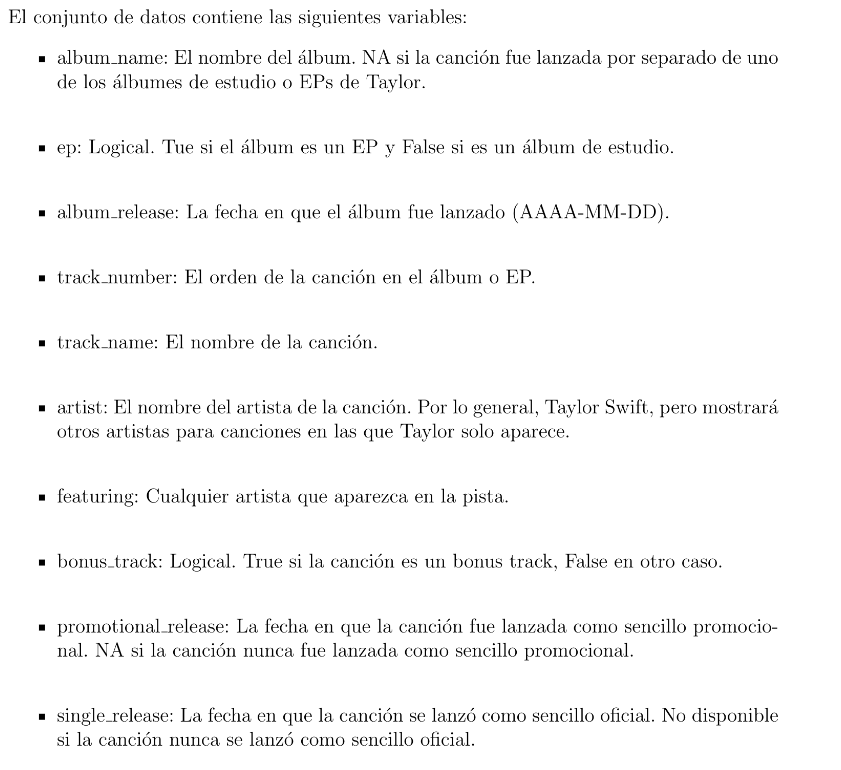
\includegraphics{songs2_var_description.png}
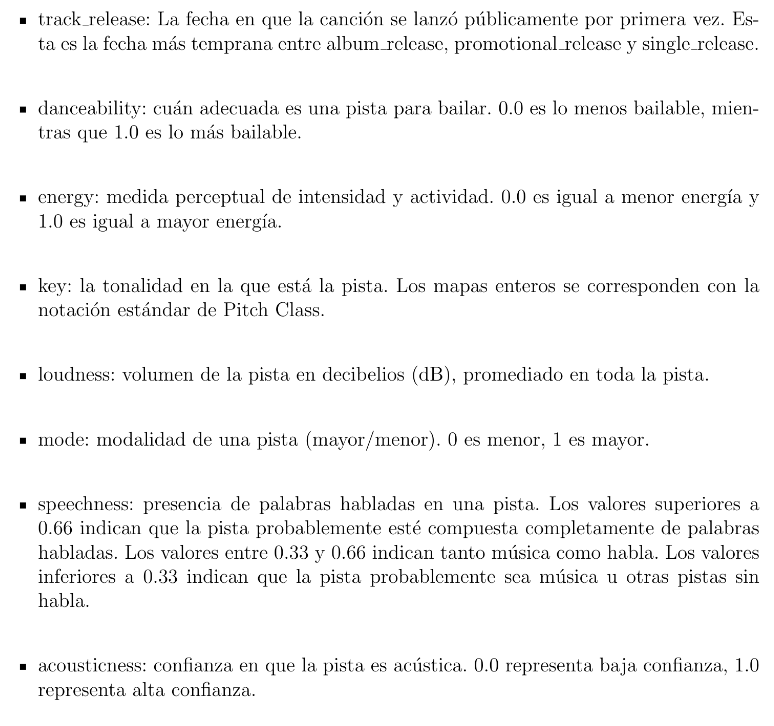
\includegraphics{songs2_var_description2.png}
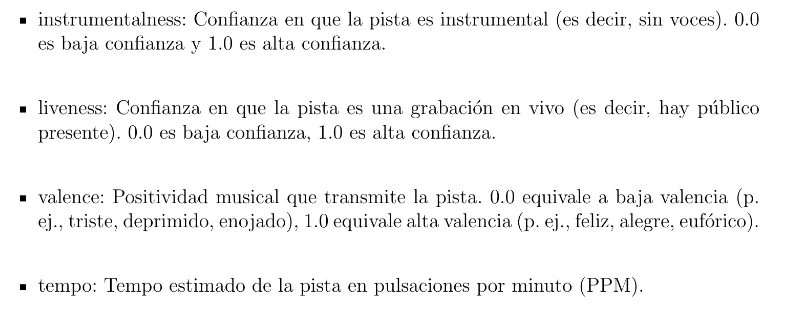
\includegraphics{songs2_var_description3.png}
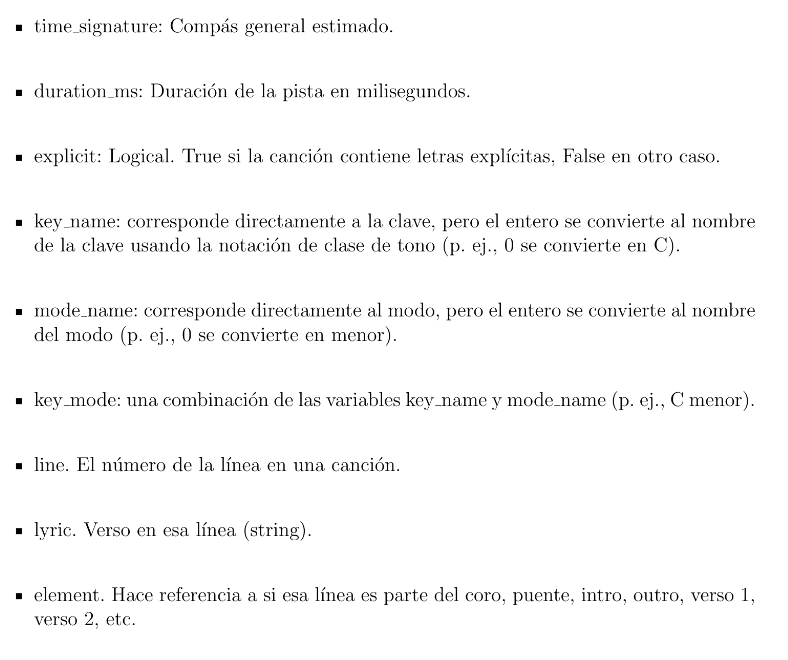
\includegraphics{songs2_var_description4.png}

    \hypertarget{actividad}{%
\subsection{Actividad}\label{actividad}}

    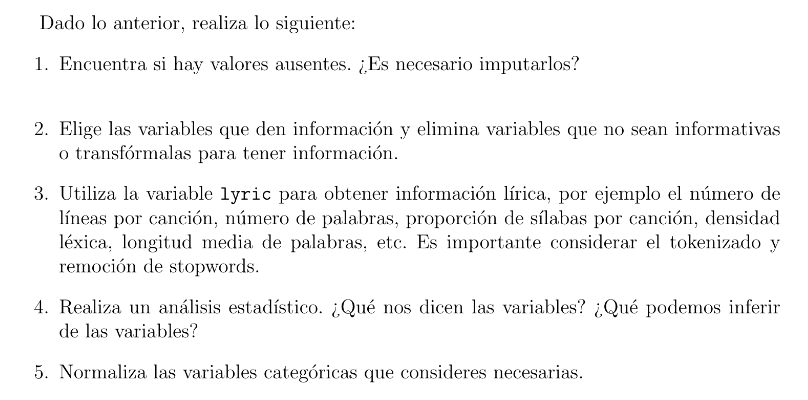
\includegraphics{songs2_activity.png}
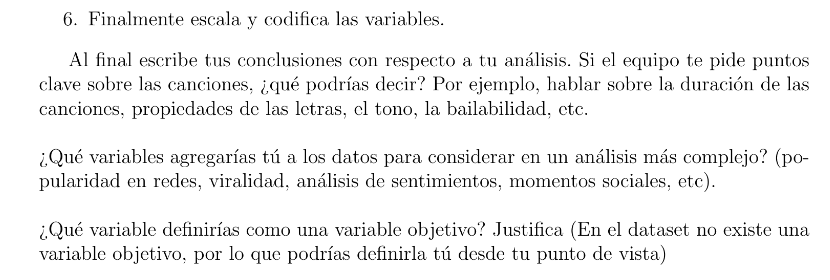
\includegraphics{songs2_activity2.png}

    \begin{tcolorbox}[breakable, size=fbox, boxrule=1pt, pad at break*=1mm,colback=cellbackground, colframe=cellborder]
\prompt{In}{incolor}{67}{\boxspacing}
\begin{Verbatim}[commandchars=\\\{\}]
\PY{n}{songs2}\PY{o}{.}\PY{n}{tail}\PY{p}{(}\PY{l+m+mi}{2}\PY{p}{)}
\end{Verbatim}
\end{tcolorbox}

            \begin{tcolorbox}[breakable, size=fbox, boxrule=.5pt, pad at break*=1mm, opacityfill=0]
\prompt{Out}{outcolor}{67}{\boxspacing}
\begin{Verbatim}[commandchars=\\\{\}]
      album\_name  ep album\_release  track\_number  \textbackslash{}
18170        NaN NaN           NaT           NaN
18171        NaN NaN           NaT           NaN

                                  track\_name          artist featuring  \textbackslash{}
18170  You'll Always Find Your Way Back Home  Hannah Montana       NaN
18171  You'll Always Find Your Way Back Home  Hannah Montana       NaN

       bonus\_track promotional\_release single\_release  {\ldots} time\_signature  \textbackslash{}
18170          NaN                 NaT     2009-03-24  {\ldots}            4.0
18171          NaN                 NaT     2009-03-24  {\ldots}            4.0

       duration\_ms  explicit  key\_name  mode\_name  key\_mode  line  \textbackslash{}
18170     224187.0       0.0        G\#      major  G\# major    58
18171     224187.0       0.0        G\#      major  G\# major    59

                                                   lyric  element  \textbackslash{}
18170         You'll always, you'll always find your way    Outro
18171  You'll always find your way (Back home) back home    Outro

       element\_artist
18170    Taylor Swift
18171    Taylor Swift

[2 rows x 32 columns]
\end{Verbatim}
\end{tcolorbox}
        
    \hypertarget{exploraciuxf3n}{%
\subsection{Exploración}\label{exploraciuxf3n}}

    \begin{tcolorbox}[breakable, size=fbox, boxrule=1pt, pad at break*=1mm,colback=cellbackground, colframe=cellborder]
\prompt{In}{incolor}{68}{\boxspacing}
\begin{Verbatim}[commandchars=\\\{\}]
\PY{n}{songs2}\PY{o}{.}\PY{n}{iloc}\PY{p}{[}\PY{p}{:}\PY{l+m+mi}{100}\PY{p}{]}\PY{o}{.}\PY{n}{to\PYZus{}csv}\PY{p}{(}\PY{l+s+s1}{\PYZsq{}}\PY{l+s+s1}{muestra\PYZus{}dataset2.csv}\PY{l+s+s1}{\PYZsq{}}\PY{p}{)}
\end{Verbatim}
\end{tcolorbox}

    \hypertarget{valores-ausentes}{%
\subsubsection{Valores ausentes}\label{valores-ausentes}}

    \begin{tcolorbox}[breakable, size=fbox, boxrule=1pt, pad at break*=1mm,colback=cellbackground, colframe=cellborder]
\prompt{In}{incolor}{69}{\boxspacing}
\begin{Verbatim}[commandchars=\\\{\}]
\PY{n}{is\PYZus{}na\PYZus{}df}\PY{p}{(}\PY{n}{songs2}\PY{p}{)}
\end{Verbatim}
\end{tcolorbox}

            \begin{tcolorbox}[breakable, size=fbox, boxrule=.5pt, pad at break*=1mm, opacityfill=0]
\prompt{Out}{outcolor}{69}{\boxspacing}
\begin{Verbatim}[commandchars=\\\{\}]
                columna  n\_missing   total  prop\_missing  prop\_original
0            album\_name       1779   18172      0.097898       0.902102
1                    ep       1779   18172      0.097898       0.902102
2         album\_release       1779   18172      0.097898       0.902102
3          track\_number       1779   18172      0.097898       0.902102
4             featuring      15898   18172      0.874862       0.125138
5           bonus\_track       1779   18172      0.097898       0.902102
6   promotional\_release      15836   18172      0.871451       0.128549
7        single\_release      14222   18172      0.782633       0.217367
8          danceability        579   18172      0.031862       0.968138
9                energy        579   18172      0.031862       0.968138
10                  key        579   18172      0.031862       0.968138
11             loudness        579   18172      0.031862       0.968138
12                 mode        579   18172      0.031862       0.968138
13          speechiness        579   18172      0.031862       0.968138
14         acousticness        579   18172      0.031862       0.968138
15     instrumentalness        579   18172      0.031862       0.968138
16             liveness        579   18172      0.031862       0.968138
17              valence        579   18172      0.031862       0.968138
18                tempo        579   18172      0.031862       0.968138
19       time\_signature        579   18172      0.031862       0.968138
20          duration\_ms        579   18172      0.031862       0.968138
21             explicit        579   18172      0.031862       0.968138
22             key\_name        579   18172      0.031862       0.968138
23            mode\_name        579   18172      0.031862       0.968138
24             key\_mode        579   18172      0.031862       0.968138
25                TOTAL      64694  581504      0.111253       0.888747
\end{Verbatim}
\end{tcolorbox}
        
    \begin{tcolorbox}[breakable, size=fbox, boxrule=1pt, pad at break*=1mm,colback=cellbackground, colframe=cellborder]
\prompt{In}{incolor}{70}{\boxspacing}
\begin{Verbatim}[commandchars=\\\{\}]
\PY{n}{is\PYZus{}na\PYZus{}df}\PY{p}{(}\PY{n}{songs2}\PY{p}{)}\PY{o}{.}\PY{n}{query}\PY{p}{(}\PY{l+s+s1}{\PYZsq{}}\PY{l+s+s1}{prop\PYZus{}missing \PYZgt{} 0.15}\PY{l+s+s1}{\PYZsq{}}\PY{p}{)}
\end{Verbatim}
\end{tcolorbox}

            \begin{tcolorbox}[breakable, size=fbox, boxrule=.5pt, pad at break*=1mm, opacityfill=0]
\prompt{Out}{outcolor}{70}{\boxspacing}
\begin{Verbatim}[commandchars=\\\{\}]
               columna  n\_missing  total  prop\_missing  prop\_original
4            featuring      15898  18172      0.874862       0.125138
6  promotional\_release      15836  18172      0.871451       0.128549
7       single\_release      14222  18172      0.782633       0.217367
\end{Verbatim}
\end{tcolorbox}
        
    \begin{tcolorbox}[breakable, size=fbox, boxrule=1pt, pad at break*=1mm,colback=cellbackground, colframe=cellborder]
\prompt{In}{incolor}{71}{\boxspacing}
\begin{Verbatim}[commandchars=\\\{\}]
\PY{n+nb}{print}\PY{p}{(}\PY{l+s+s1}{\PYZsq{}}\PY{l+s+s1}{Moda: }\PY{l+s+si}{\PYZob{}0:.2\PYZpc{}\PYZcb{}}\PY{l+s+s1}{\PYZsq{}}\PY{o}{.}\PY{n}{format}\PY{p}{(}\PY{n}{stats}\PY{o}{.}\PY{n}{mode}\PY{p}{(}\PY{n}{is\PYZus{}na\PYZus{}df}\PY{p}{(}\PY{n}{songs2}\PY{p}{)}\PY{o}{.}\PY{n}{prop\PYZus{}missing}\PY{p}{)}\PY{p}{[}\PY{l+m+mi}{0}\PY{p}{]}\PY{p}{)}\PY{p}{)}
\PY{n+nb}{print}\PY{p}{(}\PY{l+s+s1}{\PYZsq{}}\PY{l+s+s1}{Media: }\PY{l+s+si}{\PYZob{}0:.2\PYZpc{}\PYZcb{}}\PY{l+s+s1}{\PYZsq{}}\PY{o}{.}\PY{n}{format}\PY{p}{(}\PY{n}{np}\PY{o}{.}\PY{n}{mean}\PY{p}{(}\PY{n}{is\PYZus{}na\PYZus{}df}\PY{p}{(}\PY{n}{songs2}\PY{p}{)}\PY{o}{.}\PY{n}{prop\PYZus{}missing}\PY{p}{)}\PY{p}{)}\PY{p}{)}
\end{Verbatim}
\end{tcolorbox}

    \begin{Verbatim}[commandchars=\\\{\}]
Moda: 3.19\%
Media: 14.12\%
    \end{Verbatim}

    Tenemos 11\% de valores ausentes en total del dataset, la moda de
valores ausentes es de 3.19\%. La media se eleva a 14.12\% por variables
como featuring, promotional\_release y single\_release que tienen más
del 75\% de valores ausentes, vamos a revisar si es necesario eliminar
dichas variables.

    \begin{tcolorbox}[breakable, size=fbox, boxrule=1pt, pad at break*=1mm,colback=cellbackground, colframe=cellborder]
\prompt{In}{incolor}{72}{\boxspacing}
\begin{Verbatim}[commandchars=\\\{\}]
\PY{n}{dict\PYZus{}single\PYZus{}release} \PY{o}{=} \PY{p}{\PYZob{}}\PY{n}{x}\PY{p}{:} \PY{n}{i} \PY{k}{for} \PY{n}{i}\PY{p}{,} \PY{n}{x} \PY{o+ow}{in} \PY{n+nb}{enumerate}\PY{p}{(}\PY{n}{songs2}\PY{p}{[}\PY{l+s+s1}{\PYZsq{}}\PY{l+s+s1}{single\PYZus{}release}\PY{l+s+s1}{\PYZsq{}}\PY{p}{]}\PY{o}{.}\PY{n}{unique}\PY{p}{(}\PY{p}{)}\PY{o}{.}\PY{n}{dropna}\PY{p}{(}\PY{p}{)}\PY{p}{)}\PY{p}{\PYZcb{}}
\PY{n}{songs2}\PY{p}{[}\PY{l+s+s1}{\PYZsq{}}\PY{l+s+s1}{single\PYZus{}release\PYZus{}rec}\PY{l+s+s1}{\PYZsq{}}\PY{p}{]} \PY{o}{=} \PY{n}{songs2}\PY{p}{[}\PY{l+s+s1}{\PYZsq{}}\PY{l+s+s1}{single\PYZus{}release}\PY{l+s+s1}{\PYZsq{}}\PY{p}{]}\PY{o}{.}\PY{n}{map}\PY{p}{(}\PY{n}{dict\PYZus{}single\PYZus{}release}\PY{p}{)}
\PY{n}{songs2}\PY{o}{.}\PY{n}{groupby}\PY{p}{(}\PY{l+s+s1}{\PYZsq{}}\PY{l+s+s1}{track\PYZus{}name}\PY{l+s+s1}{\PYZsq{}}\PY{p}{)}\PY{p}{[}\PY{l+s+s1}{\PYZsq{}}\PY{l+s+s1}{single\PYZus{}release\PYZus{}rec}\PY{l+s+s1}{\PYZsq{}}\PY{p}{]}\PY{o}{.}\PY{n}{mean}\PY{p}{(}\PY{p}{)}\PY{o}{.}\PY{n}{map}\PY{p}{(}\PY{k}{lambda} \PY{n}{x}\PY{p}{:} \PY{l+m+mi}{1} \PY{k}{if} \PY{n}{x} \PY{o}{\PYZgt{}}\PY{o}{=} \PY{l+m+mi}{0} \PY{k}{else} \PY{l+s+s1}{\PYZsq{}}\PY{l+s+s1}{nan}\PY{l+s+s1}{\PYZsq{}}\PY{p}{)}\PY{o}{.}\PY{n}{value\PYZus{}counts}\PY{p}{(}\PY{p}{)}
\end{Verbatim}
\end{tcolorbox}

            \begin{tcolorbox}[breakable, size=fbox, boxrule=.5pt, pad at break*=1mm, opacityfill=0]
\prompt{Out}{outcolor}{72}{\boxspacing}
\begin{Verbatim}[commandchars=\\\{\}]
single\_release\_rec
nan    287
1       76
Name: count, dtype: int64
\end{Verbatim}
\end{tcolorbox}
        
    \begin{tcolorbox}[breakable, size=fbox, boxrule=1pt, pad at break*=1mm,colback=cellbackground, colframe=cellborder]
\prompt{In}{incolor}{73}{\boxspacing}
\begin{Verbatim}[commandchars=\\\{\}]
\PY{n}{dict\PYZus{}promotional\PYZus{}release} \PY{o}{=} \PY{p}{\PYZob{}}\PY{n}{x}\PY{p}{:} \PY{n}{i} \PY{k}{for} \PY{n}{i}\PY{p}{,} \PY{n}{x} \PY{o+ow}{in} \PY{n+nb}{enumerate}\PY{p}{(}\PY{n}{songs2}\PY{p}{[}\PY{l+s+s1}{\PYZsq{}}\PY{l+s+s1}{promotional\PYZus{}release}\PY{l+s+s1}{\PYZsq{}}\PY{p}{]}\PY{o}{.}\PY{n}{unique}\PY{p}{(}\PY{p}{)}\PY{o}{.}\PY{n}{dropna}\PY{p}{(}\PY{p}{)}\PY{p}{)}\PY{p}{\PYZcb{}}
\PY{n}{songs2}\PY{p}{[}\PY{l+s+s1}{\PYZsq{}}\PY{l+s+s1}{promotional\PYZus{}release\PYZus{}rec}\PY{l+s+s1}{\PYZsq{}}\PY{p}{]} \PY{o}{=} \PY{n}{songs2}\PY{p}{[}\PY{l+s+s1}{\PYZsq{}}\PY{l+s+s1}{promotional\PYZus{}release}\PY{l+s+s1}{\PYZsq{}}\PY{p}{]}\PY{o}{.}\PY{n}{map}\PY{p}{(}\PY{n}{dict\PYZus{}promotional\PYZus{}release}\PY{p}{)}
\PY{n}{songs2}\PY{o}{.}\PY{n}{groupby}\PY{p}{(}\PY{l+s+s1}{\PYZsq{}}\PY{l+s+s1}{track\PYZus{}name}\PY{l+s+s1}{\PYZsq{}}\PY{p}{)}\PY{p}{[}\PY{l+s+s1}{\PYZsq{}}\PY{l+s+s1}{promotional\PYZus{}release\PYZus{}rec}\PY{l+s+s1}{\PYZsq{}}\PY{p}{]}\PY{o}{.}\PY{n}{mean}\PY{p}{(}\PY{p}{)}\PY{o}{.}\PY{n}{map}\PY{p}{(}\PY{k}{lambda} \PY{n}{x}\PY{p}{:} \PY{l+m+mi}{1} \PY{k}{if} \PY{n}{x} \PY{o}{\PYZgt{}}\PY{o}{=} \PY{l+m+mi}{0} \PY{k}{else} \PY{l+s+s1}{\PYZsq{}}\PY{l+s+s1}{nan}\PY{l+s+s1}{\PYZsq{}}\PY{p}{)}\PY{o}{.}\PY{n}{value\PYZus{}counts}\PY{p}{(}\PY{p}{)}
\end{Verbatim}
\end{tcolorbox}

            \begin{tcolorbox}[breakable, size=fbox, boxrule=.5pt, pad at break*=1mm, opacityfill=0]
\prompt{Out}{outcolor}{73}{\boxspacing}
\begin{Verbatim}[commandchars=\\\{\}]
promotional\_release\_rec
nan    318
1       45
Name: count, dtype: int64
\end{Verbatim}
\end{tcolorbox}
        
    \begin{tcolorbox}[breakable, size=fbox, boxrule=1pt, pad at break*=1mm,colback=cellbackground, colframe=cellborder]
\prompt{In}{incolor}{74}{\boxspacing}
\begin{Verbatim}[commandchars=\\\{\}]
\PY{n}{dict\PYZus{}featuring} \PY{o}{=} \PY{p}{\PYZob{}}\PY{n}{x}\PY{p}{:} \PY{n}{i} \PY{k}{for} \PY{n}{i}\PY{p}{,} \PY{n}{x} \PY{o+ow}{in} \PY{n+nb}{enumerate}\PY{p}{(}\PY{n}{pd}\PY{o}{.}\PY{n}{Series}\PY{p}{(}\PY{n}{songs2}\PY{p}{[}\PY{l+s+s1}{\PYZsq{}}\PY{l+s+s1}{featuring}\PY{l+s+s1}{\PYZsq{}}\PY{p}{]}\PY{o}{.}\PY{n}{unique}\PY{p}{(}\PY{p}{)}\PY{p}{)}\PY{o}{.}\PY{n}{dropna}\PY{p}{(}\PY{p}{)}\PY{p}{)}\PY{p}{\PYZcb{}}

\PY{n+nb}{print}\PY{p}{(}\PY{l+s+s1}{\PYZsq{}}\PY{l+s+s1}{Artistas que cantaron con Taylor en la pista:}\PY{l+s+s1}{\PYZsq{}}\PY{p}{,} \PY{n+nb}{len}\PY{p}{(}\PY{n}{dict\PYZus{}featuring}\PY{p}{)}\PY{p}{)}

\PY{n}{songs2}\PY{p}{[}\PY{l+s+s1}{\PYZsq{}}\PY{l+s+s1}{featuring\PYZus{}rec}\PY{l+s+s1}{\PYZsq{}}\PY{p}{]} \PY{o}{=} \PY{n}{songs2}\PY{p}{[}\PY{l+s+s1}{\PYZsq{}}\PY{l+s+s1}{featuring}\PY{l+s+s1}{\PYZsq{}}\PY{p}{]}\PY{o}{.}\PY{n}{map}\PY{p}{(}\PY{n}{dict\PYZus{}featuring}\PY{p}{)}
\PY{n}{songs2}\PY{o}{.}\PY{n}{groupby}\PY{p}{(}\PY{l+s+s1}{\PYZsq{}}\PY{l+s+s1}{track\PYZus{}name}\PY{l+s+s1}{\PYZsq{}}\PY{p}{)}\PY{p}{[}\PY{l+s+s1}{\PYZsq{}}\PY{l+s+s1}{featuring\PYZus{}rec}\PY{l+s+s1}{\PYZsq{}}\PY{p}{]}\PY{o}{.}\PY{n}{mean}\PY{p}{(}\PY{p}{)}\PY{o}{.}\PY{n}{map}\PY{p}{(}\PY{k}{lambda} \PY{n}{x}\PY{p}{:} \PY{l+m+mi}{1} \PY{k}{if} \PY{n}{x} \PY{o}{\PYZgt{}}\PY{o}{=} \PY{l+m+mi}{0} \PY{k}{else} \PY{l+s+s1}{\PYZsq{}}\PY{l+s+s1}{nan}\PY{l+s+s1}{\PYZsq{}}\PY{p}{)}\PY{o}{.}\PY{n}{value\PYZus{}counts}\PY{p}{(}\PY{p}{)}
\end{Verbatim}
\end{tcolorbox}

    \begin{Verbatim}[commandchars=\\\{\}]
Artistas que cantaron con Taylor en la pista: 27
    \end{Verbatim}

            \begin{tcolorbox}[breakable, size=fbox, boxrule=.5pt, pad at break*=1mm, opacityfill=0]
\prompt{Out}{outcolor}{74}{\boxspacing}
\begin{Verbatim}[commandchars=\\\{\}]
featuring\_rec
nan    319
1       44
Name: count, dtype: int64
\end{Verbatim}
\end{tcolorbox}
        
    Los conteos anteriores confirman que conviene eliminarlas debido a su
alta concentración de valores ausentes (\textgreater15\%).

    \begin{tcolorbox}[breakable, size=fbox, boxrule=1pt, pad at break*=1mm,colback=cellbackground, colframe=cellborder]
\prompt{In}{incolor}{75}{\boxspacing}
\begin{Verbatim}[commandchars=\\\{\}]
\PY{n}{songs2}\PY{o}{.}\PY{n}{drop}\PY{p}{(}\PY{p}{[}\PY{l+s+s1}{\PYZsq{}}\PY{l+s+s1}{featuring}\PY{l+s+s1}{\PYZsq{}}\PY{p}{,}\PY{l+s+s1}{\PYZsq{}}\PY{l+s+s1}{promotional\PYZus{}release}\PY{l+s+s1}{\PYZsq{}}\PY{p}{,}\PY{l+s+s1}{\PYZsq{}}\PY{l+s+s1}{single\PYZus{}release}\PY{l+s+s1}{\PYZsq{}}\PY{p}{,}\PY{l+s+s1}{\PYZsq{}}\PY{l+s+s1}{featuring\PYZus{}rec}\PY{l+s+s1}{\PYZsq{}}\PY{p}{,}\PY{l+s+s1}{\PYZsq{}}\PY{l+s+s1}{promotional\PYZus{}release\PYZus{}rec}\PY{l+s+s1}{\PYZsq{}}\PY{p}{,}\PY{l+s+s1}{\PYZsq{}}\PY{l+s+s1}{single\PYZus{}release\PYZus{}rec}\PY{l+s+s1}{\PYZsq{}}\PY{p}{]}\PY{p}{,} \PY{n}{axis}\PY{o}{=}\PY{l+m+mi}{1}\PY{p}{,} \PY{n}{inplace}\PY{o}{=}\PY{k+kc}{True}\PY{p}{)}
\end{Verbatim}
\end{tcolorbox}

    \begin{tcolorbox}[breakable, size=fbox, boxrule=1pt, pad at break*=1mm,colback=cellbackground, colframe=cellborder]
\prompt{In}{incolor}{76}{\boxspacing}
\begin{Verbatim}[commandchars=\\\{\}]
\PY{n+nb}{print}\PY{p}{(}\PY{l+s+s1}{\PYZsq{}}\PY{l+s+s1}{Media: }\PY{l+s+si}{\PYZob{}0:.2\PYZpc{}\PYZcb{}}\PY{l+s+s1}{\PYZsq{}}\PY{o}{.}\PY{n}{format}\PY{p}{(}\PY{n}{np}\PY{o}{.}\PY{n}{mean}\PY{p}{(}\PY{n}{is\PYZus{}na\PYZus{}df}\PY{p}{(}\PY{n}{songs2}\PY{p}{)}\PY{o}{.}\PY{n}{prop\PYZus{}missing}\PY{p}{)}\PY{p}{)}\PY{p}{)}
\end{Verbatim}
\end{tcolorbox}

    \begin{Verbatim}[commandchars=\\\{\}]
Media: 4.64\%
    \end{Verbatim}

    Eliminando esas variables ya vemos que la media de valores ausentes se
asimila a la moda.

    \hypertarget{tipo-de-dato-por-variable}{%
\subsubsection{Tipo de dato por
variable}\label{tipo-de-dato-por-variable}}

    \begin{tcolorbox}[breakable, size=fbox, boxrule=1pt, pad at break*=1mm,colback=cellbackground, colframe=cellborder]
\prompt{In}{incolor}{77}{\boxspacing}
\begin{Verbatim}[commandchars=\\\{\}]
\PY{n}{songs2}\PY{o}{.}\PY{n}{info}\PY{p}{(}\PY{p}{)}
\end{Verbatim}
\end{tcolorbox}

    \begin{Verbatim}[commandchars=\\\{\}]
<class 'pandas.core.frame.DataFrame'>
RangeIndex: 18172 entries, 0 to 18171
Data columns (total 29 columns):
 \#   Column            Non-Null Count  Dtype
---  ------            --------------  -----
 0   album\_name        16393 non-null  object
 1   ep                16393 non-null  float64
 2   album\_release     16393 non-null  datetime64[ns]
 3   track\_number      16393 non-null  float64
 4   track\_name        18172 non-null  object
 5   artist            18172 non-null  object
 6   bonus\_track       16393 non-null  float64
 7   track\_release     18172 non-null  datetime64[ns]
 8   danceability      17593 non-null  float64
 9   energy            17593 non-null  float64
 10  key               17593 non-null  float64
 11  loudness          17593 non-null  float64
 12  mode              17593 non-null  float64
 13  speechiness       17593 non-null  float64
 14  acousticness      17593 non-null  float64
 15  instrumentalness  17593 non-null  float64
 16  liveness          17593 non-null  float64
 17  valence           17593 non-null  float64
 18  tempo             17593 non-null  float64
 19  time\_signature    17593 non-null  float64
 20  duration\_ms       17593 non-null  float64
 21  explicit          17593 non-null  float64
 22  key\_name          17593 non-null  object
 23  mode\_name         17593 non-null  object
 24  key\_mode          17593 non-null  object
 25  line              18172 non-null  int64
 26  lyric             18172 non-null  object
 27  element           18172 non-null  object
 28  element\_artist    18172 non-null  object
dtypes: datetime64[ns](2), float64(17), int64(1), object(9)
memory usage: 4.0+ MB
    \end{Verbatim}

    \begin{tcolorbox}[breakable, size=fbox, boxrule=1pt, pad at break*=1mm,colback=cellbackground, colframe=cellborder]
\prompt{In}{incolor}{78}{\boxspacing}
\begin{Verbatim}[commandchars=\\\{\}]
\PY{c+c1}{\PYZsh{} Clave o llave del track para agrupar líneas de letras (si hay varias filas por canción)}
\PY{n}{track\PYZus{}key} \PY{o}{=} \PY{p}{[}\PY{l+s+s2}{\PYZdq{}}\PY{l+s+s2}{artist}\PY{l+s+s2}{\PYZdq{}}\PY{p}{,}\PY{l+s+s2}{\PYZdq{}}\PY{l+s+s2}{album\PYZus{}name}\PY{l+s+s2}{\PYZdq{}}\PY{p}{,}\PY{l+s+s2}{\PYZdq{}}\PY{l+s+s2}{track\PYZus{}number}\PY{l+s+s2}{\PYZdq{}}\PY{p}{,}\PY{l+s+s2}{\PYZdq{}}\PY{l+s+s2}{track\PYZus{}name}\PY{l+s+s2}{\PYZdq{}}\PY{p}{]}
\PY{n}{track\PYZus{}key} \PY{o}{=} \PY{p}{[}\PY{n}{c} \PY{k}{for} \PY{n}{c} \PY{o+ow}{in} \PY{n}{track\PYZus{}key} \PY{k}{if} \PY{n}{c} \PY{o+ow}{in} \PY{n}{songs2}\PY{o}{.}\PY{n}{columns}\PY{p}{]}
\end{Verbatim}
\end{tcolorbox}

    \begin{tcolorbox}[breakable, size=fbox, boxrule=1pt, pad at break*=1mm,colback=cellbackground, colframe=cellborder]
\prompt{In}{incolor}{79}{\boxspacing}
\begin{Verbatim}[commandchars=\\\{\}]
\PY{n}{track\PYZus{}key}
\end{Verbatim}
\end{tcolorbox}

            \begin{tcolorbox}[breakable, size=fbox, boxrule=.5pt, pad at break*=1mm, opacityfill=0]
\prompt{Out}{outcolor}{79}{\boxspacing}
\begin{Verbatim}[commandchars=\\\{\}]
['artist', 'album\_name', 'track\_number', 'track\_name']
\end{Verbatim}
\end{tcolorbox}
        
    \begin{tcolorbox}[breakable, size=fbox, boxrule=1pt, pad at break*=1mm,colback=cellbackground, colframe=cellborder]
\prompt{In}{incolor}{80}{\boxspacing}
\begin{Verbatim}[commandchars=\\\{\}]
\PY{n}{songs2}\PY{o}{.}\PY{n}{loc}\PY{p}{[}\PY{p}{:}\PY{p}{,} \PY{n}{track\PYZus{}key}\PY{p}{]}
\end{Verbatim}
\end{tcolorbox}

            \begin{tcolorbox}[breakable, size=fbox, boxrule=.5pt, pad at break*=1mm, opacityfill=0]
\prompt{Out}{outcolor}{80}{\boxspacing}
\begin{Verbatim}[commandchars=\\\{\}]
               artist    album\_name  track\_number  \textbackslash{}
0        Taylor Swift  Taylor Swift           1.0
1        Taylor Swift  Taylor Swift           1.0
2        Taylor Swift  Taylor Swift           1.0
3        Taylor Swift  Taylor Swift           1.0
4        Taylor Swift  Taylor Swift           1.0
{\ldots}               {\ldots}           {\ldots}           {\ldots}
18167  Hannah Montana           NaN           NaN
18168  Hannah Montana           NaN           NaN
18169  Hannah Montana           NaN           NaN
18170  Hannah Montana           NaN           NaN
18171  Hannah Montana           NaN           NaN

                                  track\_name
0                                 Tim McGraw
1                                 Tim McGraw
2                                 Tim McGraw
3                                 Tim McGraw
4                                 Tim McGraw
{\ldots}                                      {\ldots}
18167  You'll Always Find Your Way Back Home
18168  You'll Always Find Your Way Back Home
18169  You'll Always Find Your Way Back Home
18170  You'll Always Find Your Way Back Home
18171  You'll Always Find Your Way Back Home

[18172 rows x 4 columns]
\end{Verbatim}
\end{tcolorbox}
        
    \begin{tcolorbox}[breakable, size=fbox, boxrule=1pt, pad at break*=1mm,colback=cellbackground, colframe=cellborder]
\prompt{In}{incolor}{81}{\boxspacing}
\begin{Verbatim}[commandchars=\\\{\}]
\PY{n}{songs2}\PY{p}{[}\PY{n}{songs2}\PY{p}{[}\PY{l+s+s1}{\PYZsq{}}\PY{l+s+s1}{track\PYZus{}name}\PY{l+s+s1}{\PYZsq{}}\PY{p}{]}\PY{o}{==}\PY{l+s+s2}{\PYZdq{}}\PY{l+s+s2}{You}\PY{l+s+s2}{\PYZsq{}}\PY{l+s+s2}{ll Always Find Your Way Back Home}\PY{l+s+s2}{\PYZdq{}}\PY{p}{]}\PY{o}{.}\PY{n}{head}\PY{p}{(}\PY{p}{)}
\end{Verbatim}
\end{tcolorbox}

            \begin{tcolorbox}[breakable, size=fbox, boxrule=.5pt, pad at break*=1mm, opacityfill=0]
\prompt{Out}{outcolor}{81}{\boxspacing}
\begin{Verbatim}[commandchars=\\\{\}]
      album\_name  ep album\_release  track\_number  \textbackslash{}
18113        NaN NaN           NaT           NaN
18114        NaN NaN           NaT           NaN
18115        NaN NaN           NaT           NaN
18116        NaN NaN           NaT           NaN
18117        NaN NaN           NaT           NaN

                                  track\_name          artist  bonus\_track  \textbackslash{}
18113  You'll Always Find Your Way Back Home  Hannah Montana          NaN
18114  You'll Always Find Your Way Back Home  Hannah Montana          NaN
18115  You'll Always Find Your Way Back Home  Hannah Montana          NaN
18116  You'll Always Find Your Way Back Home  Hannah Montana          NaN
18117  You'll Always Find Your Way Back Home  Hannah Montana          NaN

      track\_release  danceability  energy  {\ldots}  time\_signature  duration\_ms  \textbackslash{}
18113    2009-03-24         0.577   0.906  {\ldots}             4.0     224187.0
18114    2009-03-24         0.577   0.906  {\ldots}             4.0     224187.0
18115    2009-03-24         0.577   0.906  {\ldots}             4.0     224187.0
18116    2009-03-24         0.577   0.906  {\ldots}             4.0     224187.0
18117    2009-03-24         0.577   0.906  {\ldots}             4.0     224187.0

       explicit  key\_name  mode\_name  key\_mode  line  \textbackslash{}
18113       0.0        G\#      major  G\# major     1
18114       0.0        G\#      major  G\# major     2
18115       0.0        G\#      major  G\# major     3
18116       0.0        G\#      major  G\# major     4
18117       0.0        G\#      major  G\# major     5

                                    lyric  element  element\_artist
18113                                Woo!    Intro    Taylor Swift
18114                         You wake up  Verse 1    Taylor Swift
18115        It's raining and it's Monday  Verse 1    Taylor Swift
18116  Looks like one of those rough days  Verse 1    Taylor Swift
18117                           Time's up  Verse 1    Taylor Swift

[5 rows x 29 columns]
\end{Verbatim}
\end{tcolorbox}
        
    \begin{tcolorbox}[breakable, size=fbox, boxrule=1pt, pad at break*=1mm,colback=cellbackground, colframe=cellborder]
\prompt{In}{incolor}{82}{\boxspacing}
\begin{Verbatim}[commandchars=\\\{\}]
\PY{n}{songs2}\PY{p}{[}\PY{n}{songs2}\PY{p}{[}\PY{l+s+s1}{\PYZsq{}}\PY{l+s+s1}{track\PYZus{}name}\PY{l+s+s1}{\PYZsq{}}\PY{p}{]}\PY{o}{==}\PY{l+s+s2}{\PYZdq{}}\PY{l+s+s2}{You}\PY{l+s+s2}{\PYZsq{}}\PY{l+s+s2}{ll Always Find Your Way Back Home}\PY{l+s+s2}{\PYZdq{}}\PY{p}{]}\PY{o}{.}\PY{n}{shape}
\end{Verbatim}
\end{tcolorbox}

            \begin{tcolorbox}[breakable, size=fbox, boxrule=.5pt, pad at break*=1mm, opacityfill=0]
\prompt{Out}{outcolor}{82}{\boxspacing}
\begin{Verbatim}[commandchars=\\\{\}]
(59, 29)
\end{Verbatim}
\end{tcolorbox}
        
    \begin{tcolorbox}[breakable, size=fbox, boxrule=1pt, pad at break*=1mm,colback=cellbackground, colframe=cellborder]
\prompt{In}{incolor}{83}{\boxspacing}
\begin{Verbatim}[commandchars=\\\{\}]
\PY{n}{songs2}\PY{p}{[}\PY{n}{songs2}\PY{p}{[}\PY{l+s+s1}{\PYZsq{}}\PY{l+s+s1}{track\PYZus{}name}\PY{l+s+s1}{\PYZsq{}}\PY{p}{]}\PY{o}{==}\PY{l+s+s2}{\PYZdq{}}\PY{l+s+s2}{You}\PY{l+s+s2}{\PYZsq{}}\PY{l+s+s2}{ll Always Find Your Way Back Home}\PY{l+s+s2}{\PYZdq{}}\PY{p}{]}\PY{p}{[}\PY{l+s+s1}{\PYZsq{}}\PY{l+s+s1}{line}\PY{l+s+s1}{\PYZsq{}}\PY{p}{]}\PY{o}{.}\PY{n}{max}\PY{p}{(}\PY{p}{)}
\end{Verbatim}
\end{tcolorbox}

            \begin{tcolorbox}[breakable, size=fbox, boxrule=.5pt, pad at break*=1mm, opacityfill=0]
\prompt{Out}{outcolor}{83}{\boxspacing}
\begin{Verbatim}[commandchars=\\\{\}]
59
\end{Verbatim}
\end{tcolorbox}
        
    El dataset viene a nivel lírica o línea de cada canción por lo que
establecimos `artist', `album\_name', `track\_number', `track\_name'
como la llave para agrupar y obtener las características o métricas de
cada canción para poder clusterizar.

    \begin{tcolorbox}[breakable, size=fbox, boxrule=1pt, pad at break*=1mm,colback=cellbackground, colframe=cellborder]
\prompt{In}{incolor}{84}{\boxspacing}
\begin{Verbatim}[commandchars=\\\{\}]
\PY{n}{songs2}\PY{o}{.}\PY{n}{query}\PY{p}{(}\PY{l+s+s2}{\PYZdq{}}\PY{l+s+s2}{artist == }\PY{l+s+s2}{\PYZsq{}}\PY{l+s+s2}{Taylor Swift}\PY{l+s+s2}{\PYZsq{}}\PY{l+s+s2}{\PYZdq{}}\PY{p}{,} \PY{n}{inplace}\PY{o}{=}\PY{k+kc}{True}\PY{p}{)} \PY{c+c1}{\PYZsh{} canciones de taylor swift como artista principal}
\end{Verbatim}
\end{tcolorbox}

    \begin{tcolorbox}[breakable, size=fbox, boxrule=1pt, pad at break*=1mm,colback=cellbackground, colframe=cellborder]
\prompt{In}{incolor}{85}{\boxspacing}
\begin{Verbatim}[commandchars=\\\{\}]
\PY{n}{songs2}\PY{p}{[}\PY{l+s+s1}{\PYZsq{}}\PY{l+s+s1}{artist}\PY{l+s+s1}{\PYZsq{}}\PY{p}{]}\PY{o}{.}\PY{n}{unique}\PY{p}{(}\PY{p}{)} \PY{c+c1}{\PYZsh{} validación que sólo traigamos a Taylor como artista}
\end{Verbatim}
\end{tcolorbox}

            \begin{tcolorbox}[breakable, size=fbox, boxrule=.5pt, pad at break*=1mm, opacityfill=0]
\prompt{Out}{outcolor}{85}{\boxspacing}
\begin{Verbatim}[commandchars=\\\{\}]
array(['Taylor Swift'], dtype=object)
\end{Verbatim}
\end{tcolorbox}
        
    \begin{tcolorbox}[breakable, size=fbox, boxrule=1pt, pad at break*=1mm,colback=cellbackground, colframe=cellborder]
\prompt{In}{incolor}{86}{\boxspacing}
\begin{Verbatim}[commandchars=\\\{\}]
\PY{n}{songs2}\PY{o}{.}\PY{n}{shape} \PY{c+c1}{\PYZsh{} dimensión}
\end{Verbatim}
\end{tcolorbox}

            \begin{tcolorbox}[breakable, size=fbox, boxrule=.5pt, pad at break*=1mm, opacityfill=0]
\prompt{Out}{outcolor}{86}{\boxspacing}
\begin{Verbatim}[commandchars=\\\{\}]
(17204, 29)
\end{Verbatim}
\end{tcolorbox}
        
    \hypertarget{tratamiento-de-datos}{%
\subsection{Tratamiento de Datos}\label{tratamiento-de-datos}}

    \hypertarget{funciones-para-obtener-muxe9tricas-de-la-letra-y-canciones}{%
\subsubsection{Funciones para obtener métricas de la letra y
canciones}\label{funciones-para-obtener-muxe9tricas-de-la-letra-y-canciones}}

    \begin{tcolorbox}[breakable, size=fbox, boxrule=1pt, pad at break*=1mm,colback=cellbackground, colframe=cellborder]
\prompt{In}{incolor}{87}{\boxspacing}
\begin{Verbatim}[commandchars=\\\{\}]
\PY{c+c1}{\PYZsh{} instalar en primera ejecución}
\PY{c+c1}{\PYZsh{} nltk.download(\PYZdq{}stopwords\PYZdq{}); nltk.download(\PYZdq{}punkt\PYZdq{}); nltk.download(\PYZsq{}punkt\PYZus{}tab\PYZsq{})}
\end{Verbatim}
\end{tcolorbox}

    \begin{tcolorbox}[breakable, size=fbox, boxrule=1pt, pad at break*=1mm,colback=cellbackground, colframe=cellborder]
\prompt{In}{incolor}{88}{\boxspacing}
\begin{Verbatim}[commandchars=\\\{\}]
\PY{c+c1}{\PYZsh{} campos principales (llave) por canción}
\PY{n}{track\PYZus{}key} \PY{o}{=} \PY{p}{[}\PY{n}{c} \PY{k}{for} \PY{n}{c} \PY{o+ow}{in} \PY{p}{[}\PY{l+s+s2}{\PYZdq{}}\PY{l+s+s2}{artist}\PY{l+s+s2}{\PYZdq{}}\PY{p}{,}\PY{l+s+s2}{\PYZdq{}}\PY{l+s+s2}{album\PYZus{}name}\PY{l+s+s2}{\PYZdq{}}\PY{p}{,}\PY{l+s+s2}{\PYZdq{}}\PY{l+s+s2}{track\PYZus{}number}\PY{l+s+s2}{\PYZdq{}}\PY{p}{,}\PY{l+s+s2}{\PYZdq{}}\PY{l+s+s2}{track\PYZus{}name}\PY{l+s+s2}{\PYZdq{}}\PY{p}{]} \PY{k}{if} \PY{n}{c} \PY{o+ow}{in} \PY{n}{songs2}\PY{o}{.}\PY{n}{columns}\PY{p}{]}

\PY{c+c1}{\PYZsh{} stopwords y vocales}
\PY{n}{stop\PYZus{}es} \PY{o}{=} \PY{n+nb}{set}\PY{p}{(}\PY{n}{stopwords}\PY{o}{.}\PY{n}{words}\PY{p}{(}\PY{l+s+s2}{\PYZdq{}}\PY{l+s+s2}{spanish}\PY{l+s+s2}{\PYZdq{}}\PY{p}{)}\PY{p}{)}
\PY{n}{stop\PYZus{}en} \PY{o}{=} \PY{n+nb}{set}\PY{p}{(}\PY{n}{stopwords}\PY{o}{.}\PY{n}{words}\PY{p}{(}\PY{l+s+s2}{\PYZdq{}}\PY{l+s+s2}{english}\PY{l+s+s2}{\PYZdq{}}\PY{p}{)}\PY{p}{)}
\PY{n}{stop\PYZus{}all} \PY{o}{=} \PY{n}{stop\PYZus{}es} \PY{o}{|} \PY{n}{stop\PYZus{}en}

\PY{n}{\PYZus{}vowels} \PY{o}{=} \PY{n}{re}\PY{o}{.}\PY{n}{compile}\PY{p}{(}\PY{l+s+sa}{r}\PY{l+s+s2}{\PYZdq{}}\PY{l+s+s2}{[aeiouáéíóúü]+}\PY{l+s+s2}{\PYZdq{}}\PY{p}{,} \PY{n}{re}\PY{o}{.}\PY{n}{IGNORECASE}\PY{p}{)}

\PY{k}{def} \PY{n+nf}{count\PYZus{}syllables}\PY{p}{(}\PY{n}{word}\PY{p}{:} \PY{n+nb}{str}\PY{p}{)} \PY{o}{\PYZhy{}}\PY{o}{\PYZgt{}} \PY{n+nb}{int}\PY{p}{:}
    \PY{k}{return} \PY{n+nb}{max}\PY{p}{(}\PY{l+m+mi}{1}\PY{p}{,} \PY{n+nb}{len}\PY{p}{(}\PY{n}{\PYZus{}vowels}\PY{o}{.}\PY{n}{findall}\PY{p}{(}\PY{n}{word}\PY{p}{)}\PY{p}{)}\PY{p}{)}

\PY{k}{def} \PY{n+nf}{text\PYZus{}features}\PY{p}{(}\PY{n}{s}\PY{p}{:} \PY{n+nb}{str}\PY{p}{)} \PY{o}{\PYZhy{}}\PY{o}{\PYZgt{}} \PY{n+nb}{dict}\PY{p}{:}
    \PY{k}{if} \PY{o+ow}{not} \PY{n+nb}{isinstance}\PY{p}{(}\PY{n}{s}\PY{p}{,} \PY{n+nb}{str}\PY{p}{)} \PY{o+ow}{or} \PY{o+ow}{not} \PY{n}{s}\PY{o}{.}\PY{n}{strip}\PY{p}{(}\PY{p}{)}\PY{p}{:}
        \PY{k}{return} \PY{p}{\PYZob{}}\PY{l+s+s2}{\PYZdq{}}\PY{l+s+s2}{n\PYZus{}words}\PY{l+s+s2}{\PYZdq{}}\PY{p}{:}\PY{l+m+mi}{0}\PY{p}{,}\PY{l+s+s2}{\PYZdq{}}\PY{l+s+s2}{n\PYZus{}unique}\PY{l+s+s2}{\PYZdq{}}\PY{p}{:}\PY{l+m+mi}{0}\PY{p}{,}\PY{l+s+s2}{\PYZdq{}}\PY{l+s+s2}{lex\PYZus{}density}\PY{l+s+s2}{\PYZdq{}}\PY{p}{:}\PY{l+m+mf}{0.0}\PY{p}{,}\PY{l+s+s2}{\PYZdq{}}\PY{l+s+s2}{avg\PYZus{}word\PYZus{}len}\PY{l+s+s2}{\PYZdq{}}\PY{p}{:}\PY{l+m+mf}{0.0}\PY{p}{,}\PY{l+s+s2}{\PYZdq{}}\PY{l+s+s2}{avg\PYZus{}syllables}\PY{l+s+s2}{\PYZdq{}}\PY{p}{:}\PY{l+m+mf}{0.0}\PY{p}{,}\PY{l+s+s2}{\PYZdq{}}\PY{l+s+s2}{stop\PYZus{}ratio}\PY{l+s+s2}{\PYZdq{}}\PY{p}{:}\PY{l+m+mf}{0.0}\PY{p}{\PYZcb{}}
    \PY{n}{toks} \PY{o}{=} \PY{p}{[}\PY{n}{t}\PY{o}{.}\PY{n}{lower}\PY{p}{(}\PY{p}{)} \PY{k}{for} \PY{n}{t} \PY{o+ow}{in} \PY{n}{word\PYZus{}tokenize}\PY{p}{(}\PY{n}{s}\PY{p}{)} \PY{k}{if} \PY{n}{re}\PY{o}{.}\PY{n}{match}\PY{p}{(}\PY{l+s+sa}{r}\PY{l+s+s2}{\PYZdq{}}\PY{l+s+s2}{\PYZbs{}}\PY{l+s+s2}{w+}\PY{l+s+s2}{\PYZdq{}}\PY{p}{,} \PY{n}{t}\PY{p}{)}\PY{p}{]}
    \PY{k}{if} \PY{o+ow}{not} \PY{n}{toks}\PY{p}{:}
        \PY{k}{return} \PY{p}{\PYZob{}}\PY{l+s+s2}{\PYZdq{}}\PY{l+s+s2}{n\PYZus{}words}\PY{l+s+s2}{\PYZdq{}}\PY{p}{:}\PY{l+m+mi}{0}\PY{p}{,}\PY{l+s+s2}{\PYZdq{}}\PY{l+s+s2}{n\PYZus{}unique}\PY{l+s+s2}{\PYZdq{}}\PY{p}{:}\PY{l+m+mi}{0}\PY{p}{,}\PY{l+s+s2}{\PYZdq{}}\PY{l+s+s2}{lex\PYZus{}density}\PY{l+s+s2}{\PYZdq{}}\PY{p}{:}\PY{l+m+mf}{0.0}\PY{p}{,}\PY{l+s+s2}{\PYZdq{}}\PY{l+s+s2}{avg\PYZus{}word\PYZus{}len}\PY{l+s+s2}{\PYZdq{}}\PY{p}{:}\PY{l+m+mf}{0.0}\PY{p}{,}\PY{l+s+s2}{\PYZdq{}}\PY{l+s+s2}{avg\PYZus{}syllables}\PY{l+s+s2}{\PYZdq{}}\PY{p}{:}\PY{l+m+mf}{0.0}\PY{p}{,}\PY{l+s+s2}{\PYZdq{}}\PY{l+s+s2}{stop\PYZus{}ratio}\PY{l+s+s2}{\PYZdq{}}\PY{p}{:}\PY{l+m+mf}{0.0}\PY{p}{\PYZcb{}}

    \PY{n}{n\PYZus{}words} \PY{o}{=} \PY{n+nb}{len}\PY{p}{(}\PY{n}{toks}\PY{p}{)}
    \PY{n}{unique} \PY{o}{=} \PY{n+nb}{len}\PY{p}{(}\PY{n+nb}{set}\PY{p}{(}\PY{n}{toks}\PY{p}{)}\PY{p}{)}
    \PY{n}{avg\PYZus{}len} \PY{o}{=} \PY{n+nb}{float}\PY{p}{(}\PY{n}{np}\PY{o}{.}\PY{n}{mean}\PY{p}{(}\PY{p}{[}\PY{n+nb}{len}\PY{p}{(}\PY{n}{w}\PY{p}{)} \PY{k}{for} \PY{n}{w} \PY{o+ow}{in} \PY{n}{toks}\PY{p}{]}\PY{p}{)}\PY{p}{)}
    \PY{n}{avg\PYZus{}syl} \PY{o}{=} \PY{n+nb}{float}\PY{p}{(}\PY{n}{np}\PY{o}{.}\PY{n}{mean}\PY{p}{(}\PY{p}{[}\PY{n}{count\PYZus{}syllables}\PY{p}{(}\PY{n}{w}\PY{p}{)} \PY{k}{for} \PY{n}{w} \PY{o+ow}{in} \PY{n}{toks}\PY{p}{]}\PY{p}{)}\PY{p}{)}
    \PY{n}{n\PYZus{}stop} \PY{o}{=} \PY{n+nb}{sum}\PY{p}{(}\PY{n}{w} \PY{o+ow}{in} \PY{n}{stop\PYZus{}all} \PY{k}{for} \PY{n}{w} \PY{o+ow}{in} \PY{n}{toks}\PY{p}{)}
    \PY{n}{lex\PYZus{}density} \PY{o}{=} \PY{l+m+mi}{1} \PY{o}{\PYZhy{}} \PY{p}{(}\PY{n}{n\PYZus{}stop} \PY{o}{/} \PY{n}{n\PYZus{}words}\PY{p}{)}
    \PY{n}{stop\PYZus{}ratio} \PY{o}{=} \PY{n}{n\PYZus{}stop} \PY{o}{/} \PY{n}{n\PYZus{}words}

    \PY{k}{return} \PY{p}{\PYZob{}}
        \PY{l+s+s2}{\PYZdq{}}\PY{l+s+s2}{n\PYZus{}words}\PY{l+s+s2}{\PYZdq{}}\PY{p}{:} \PY{n}{n\PYZus{}words}\PY{p}{,}
        \PY{l+s+s2}{\PYZdq{}}\PY{l+s+s2}{n\PYZus{}unique}\PY{l+s+s2}{\PYZdq{}}\PY{p}{:} \PY{n}{unique}\PY{p}{,}
        \PY{l+s+s2}{\PYZdq{}}\PY{l+s+s2}{lex\PYZus{}density}\PY{l+s+s2}{\PYZdq{}}\PY{p}{:} \PY{n}{lex\PYZus{}density}\PY{p}{,}
        \PY{l+s+s2}{\PYZdq{}}\PY{l+s+s2}{avg\PYZus{}word\PYZus{}len}\PY{l+s+s2}{\PYZdq{}}\PY{p}{:} \PY{n}{avg\PYZus{}len}\PY{p}{,}
        \PY{l+s+s2}{\PYZdq{}}\PY{l+s+s2}{avg\PYZus{}syllables}\PY{l+s+s2}{\PYZdq{}}\PY{p}{:} \PY{n}{avg\PYZus{}syl}\PY{p}{,}
        \PY{l+s+s2}{\PYZdq{}}\PY{l+s+s2}{stop\PYZus{}ratio}\PY{l+s+s2}{\PYZdq{}}\PY{p}{:} \PY{n}{stop\PYZus{}ratio}\PY{p}{,}
    \PY{p}{\PYZcb{}}
\end{Verbatim}
\end{tcolorbox}

    \begin{tcolorbox}[breakable, size=fbox, boxrule=1pt, pad at break*=1mm,colback=cellbackground, colframe=cellborder]
\prompt{In}{incolor}{89}{\boxspacing}
\begin{Verbatim}[commandchars=\\\{\}]
\PY{c+c1}{\PYZsh{} Métricas de letra por canción}

\PY{n}{agg\PYZus{}text} \PY{o}{=} \PY{p}{(} 
    \PY{n}{songs2}\PY{o}{.}\PY{n}{groupby}\PY{p}{(}\PY{n}{track\PYZus{}key}\PY{p}{)}\PY{p}{[}\PY{l+s+s2}{\PYZdq{}}\PY{l+s+s2}{lyric}\PY{l+s+s2}{\PYZdq{}}\PY{p}{]} 
      \PY{o}{.}\PY{n}{apply}\PY{p}{(}\PY{k}{lambda} \PY{n}{s}\PY{p}{:} \PY{l+s+s2}{\PYZdq{}}\PY{l+s+se}{\PYZbs{}n}\PY{l+s+s2}{\PYZdq{}}\PY{o}{.}\PY{n}{join}\PY{p}{(}\PY{n}{s}\PY{o}{.}\PY{n}{dropna}\PY{p}{(}\PY{p}{)}\PY{o}{.}\PY{n}{astype}\PY{p}{(}\PY{n+nb}{str}\PY{p}{)}\PY{p}{)}\PY{p}{)}  \PY{c+c1}{\PYZsh{} concatenar letra completa}
      \PY{o}{.}\PY{n}{reset\PYZus{}index}\PY{p}{(}\PY{p}{)}
\PY{p}{)}

\PY{n}{agg\PYZus{}text}\PY{p}{[}\PY{l+s+s2}{\PYZdq{}}\PY{l+s+s2}{n\PYZus{}lines}\PY{l+s+s2}{\PYZdq{}}\PY{p}{]} \PY{o}{=} \PY{n}{agg\PYZus{}text}\PY{p}{[}\PY{l+s+s2}{\PYZdq{}}\PY{l+s+s2}{lyric}\PY{l+s+s2}{\PYZdq{}}\PY{p}{]}\PY{o}{.}\PY{n}{str}\PY{o}{.}\PY{n}{count}\PY{p}{(}\PY{l+s+sa}{r}\PY{l+s+s2}{\PYZdq{}}\PY{l+s+s2}{\PYZbs{}}\PY{l+s+s2}{n}\PY{l+s+s2}{\PYZdq{}}\PY{p}{)}\PY{o}{.}\PY{n}{fillna}\PY{p}{(}\PY{l+m+mi}{0}\PY{p}{)}\PY{o}{.}\PY{n}{astype}\PY{p}{(}\PY{n+nb}{int}\PY{p}{)} \PY{c+c1}{\PYZsh{} líneas por canción}
\PY{n}{agg\PYZus{}text\PYZus{}feats} \PY{o}{=} \PY{n}{agg\PYZus{}text}\PY{p}{[}\PY{l+s+s2}{\PYZdq{}}\PY{l+s+s2}{lyric}\PY{l+s+s2}{\PYZdq{}}\PY{p}{]}\PY{o}{.}\PY{n}{apply}\PY{p}{(}\PY{n}{text\PYZus{}features}\PY{p}{)}\PY{o}{.}\PY{n}{apply}\PY{p}{(}\PY{n}{pd}\PY{o}{.}\PY{n}{Series}\PY{p}{)} \PY{c+c1}{\PYZsh{} features de la letra}
\PY{n}{agg\PYZus{}text}\PY{p}{[}\PY{l+s+s2}{\PYZdq{}}\PY{l+s+s2}{lyric}\PY{l+s+s2}{\PYZdq{}}\PY{p}{]} \PY{o}{=} \PY{n}{agg\PYZus{}text}\PY{p}{[}\PY{l+s+s2}{\PYZdq{}}\PY{l+s+s2}{lyric}\PY{l+s+s2}{\PYZdq{}}\PY{p}{]}\PY{o}{.}\PY{n}{str}\PY{o}{.}\PY{n}{replace}\PY{p}{(}\PY{l+s+s1}{\PYZsq{}}\PY{l+s+se}{\PYZbs{}n}\PY{l+s+s1}{\PYZsq{}}\PY{p}{,} \PY{l+s+s1}{\PYZsq{}}\PY{l+s+s1}{ }\PY{l+s+s1}{\PYZsq{}}\PY{p}{)} \PY{c+c1}{\PYZsh{} sustituir saltos de línea por espacios}
\PY{n}{agg\PYZus{}text} \PY{o}{=} \PY{n}{pd}\PY{o}{.}\PY{n}{concat}\PY{p}{(}\PY{p}{[}\PY{n}{agg\PYZus{}text}\PY{p}{[}\PY{n}{track\PYZus{}key} \PY{o}{+} \PY{p}{[}\PY{l+s+s1}{\PYZsq{}}\PY{l+s+s1}{lyric}\PY{l+s+s1}{\PYZsq{}}\PY{p}{,}\PY{l+s+s1}{\PYZsq{}}\PY{l+s+s1}{n\PYZus{}lines}\PY{l+s+s1}{\PYZsq{}}\PY{p}{]}\PY{p}{]}\PY{p}{,} \PY{n}{agg\PYZus{}text\PYZus{}feats}\PY{p}{]}\PY{p}{,} \PY{n}{axis}\PY{o}{=}\PY{l+m+mi}{1}\PY{p}{)} \PY{c+c1}{\PYZsh{} concatenar features de la letra por canción}

\PY{n+nb}{print}\PY{p}{(}\PY{l+s+s1}{\PYZsq{}}\PY{l+s+s1}{Dimensión}\PY{l+s+s1}{\PYZsq{}}\PY{p}{,} \PY{n}{agg\PYZus{}text}\PY{o}{.}\PY{n}{shape}\PY{p}{,} \PY{n}{end}\PY{o}{=}\PY{l+s+s1}{\PYZsq{}}\PY{l+s+se}{\PYZbs{}n}\PY{l+s+se}{\PYZbs{}n}\PY{l+s+s1}{\PYZsq{}}\PY{p}{)}
\PY{n}{display}\PY{p}{(}\PY{n}{agg\PYZus{}text}\PY{o}{.}\PY{n}{head}\PY{p}{(}\PY{l+m+mi}{3}\PY{p}{)}\PY{p}{)}
\end{Verbatim}
\end{tcolorbox}

    \begin{Verbatim}[commandchars=\\\{\}]
Dimensión (326, 12)

    \end{Verbatim}

    
    \begin{Verbatim}[commandchars=\\\{\}]
         artist album\_name  track\_number           track\_name  \textbackslash{}
0  Taylor Swift       1989           1.0  Welcome To New York   
1  Taylor Swift       1989           2.0          Blank Space   
2  Taylor Swift       1989           3.0                Style   

                                               lyric  n\_lines  n\_words  \textbackslash{}
0  Walking through a crowd, the village is aglow {\ldots}       43    348.0   
1  Nice to meet you, where you been? I could show{\ldots}       83    509.0   
2  Midnight You come and pick me up, no headlight{\ldots}       47    383.0   

   n\_unique  lex\_density  avg\_word\_len  avg\_syllables  stop\_ratio  
0      91.0     0.557471      4.135057       1.399425    0.442529  
1     175.0     0.514735      3.555992       1.249509    0.485265  
2     120.0     0.522193      3.605744       1.245431    0.477807  
    \end{Verbatim}

    
    \begin{tcolorbox}[breakable, size=fbox, boxrule=1pt, pad at break*=1mm,colback=cellbackground, colframe=cellborder]
\prompt{In}{incolor}{90}{\boxspacing}
\begin{Verbatim}[commandchars=\\\{\}]
\PY{c+c1}{\PYZsh{} Proporción de elementos (coro, verso, intro…)}
\PY{n}{elem\PYZus{}props} \PY{o}{=} \PY{p}{(}
    \PY{n}{songs2}\PY{o}{.}\PY{n}{groupby}\PY{p}{(}\PY{n}{track\PYZus{}key} \PY{o}{+} \PY{p}{[}\PY{l+s+s2}{\PYZdq{}}\PY{l+s+s2}{element}\PY{l+s+s2}{\PYZdq{}}\PY{p}{]}\PY{p}{)}\PY{o}{.}\PY{n}{size}\PY{p}{(}\PY{p}{)}\PY{o}{.}\PY{n}{unstack}\PY{p}{(}\PY{n}{fill\PYZus{}value}\PY{o}{=}\PY{l+m+mi}{0}\PY{p}{)}
\PY{p}{)}
\PY{n}{elem\PYZus{}props} \PY{o}{=} \PY{n}{elem\PYZus{}props}\PY{o}{.}\PY{n}{div}\PY{p}{(}\PY{n}{elem\PYZus{}props}\PY{o}{.}\PY{n}{sum}\PY{p}{(}\PY{n}{axis}\PY{o}{=}\PY{l+m+mi}{1}\PY{p}{)}\PY{p}{,} \PY{n}{axis}\PY{o}{=}\PY{l+m+mi}{0}\PY{p}{)}  \PY{c+c1}{\PYZsh{} normalizar a proporciones}
\PY{n}{elem\PYZus{}props}\PY{o}{.}\PY{n}{columns} \PY{o}{=} \PY{p}{[}\PY{l+s+sa}{f}\PY{l+s+s2}{\PYZdq{}}\PY{l+s+s2}{elem\PYZus{}prop\PYZus{}}\PY{l+s+si}{\PYZob{}}\PY{n}{c}\PY{l+s+si}{\PYZcb{}}\PY{l+s+s2}{\PYZdq{}} \PY{k}{for} \PY{n}{c} \PY{o+ow}{in} \PY{n}{elem\PYZus{}props}\PY{o}{.}\PY{n}{columns}\PY{p}{]}

\PY{n+nb}{print}\PY{p}{(}\PY{l+s+s1}{\PYZsq{}}\PY{l+s+s1}{Dimensión}\PY{l+s+s1}{\PYZsq{}}\PY{p}{,} \PY{n}{elem\PYZus{}props}\PY{o}{.}\PY{n}{shape}\PY{p}{,} \PY{n}{end}\PY{o}{=}\PY{l+s+s1}{\PYZsq{}}\PY{l+s+se}{\PYZbs{}n}\PY{l+s+se}{\PYZbs{}n}\PY{l+s+s1}{\PYZsq{}}\PY{p}{)}
\PY{n}{display}\PY{p}{(}\PY{n}{elem\PYZus{}props}\PY{o}{.}\PY{n}{head}\PY{p}{(}\PY{l+m+mi}{3}\PY{p}{)}\PY{p}{)}
\end{Verbatim}
\end{tcolorbox}

    \begin{Verbatim}[commandchars=\\\{\}]
Dimensión (326, 29)

    \end{Verbatim}

    
    \begin{Verbatim}[commandchars=\\\{\}]
                                                          elem\_prop\_Break  \textbackslash{}
artist       album\_name track\_number track\_name                             
Taylor Swift 1989       1.0          Welcome To New York              0.0   
                        2.0          Blank Space                      0.0   
                        3.0          Style                            0.0   

                                                          elem\_prop\_Breakdown  \textbackslash{}
artist       album\_name track\_number track\_name                                 
Taylor Swift 1989       1.0          Welcome To New York                  0.0   
                        2.0          Blank Space                          0.0   
                        3.0          Style                                0.0   

                                                          elem\_prop\_Bridge  \textbackslash{}
artist       album\_name track\_number track\_name                              
Taylor Swift 1989       1.0          Welcome To New York          0.090909   
                        2.0          Blank Space                  0.047619   
                        3.0          Style                        0.104167   

                                                          elem\_prop\_Bridge 1  \textbackslash{}
artist       album\_name track\_number track\_name                                
Taylor Swift 1989       1.0          Welcome To New York                 0.0   
                        2.0          Blank Space                         0.0   
                        3.0          Style                               0.0   

                                                          elem\_prop\_Bridge 2  \textbackslash{}
artist       album\_name track\_number track\_name                                
Taylor Swift 1989       1.0          Welcome To New York                 0.0   
                        2.0          Blank Space                         0.0   
                        3.0          Style                               0.0   

                                                          elem\_prop\_Buildup  \textbackslash{}
artist       album\_name track\_number track\_name                               
Taylor Swift 1989       1.0          Welcome To New York                0.0   
                        2.0          Blank Space                        0.0   
                        3.0          Style                              0.0   

                                                          elem\_prop\_Chorus  \textbackslash{}
artist       album\_name track\_number track\_name                              
Taylor Swift 1989       1.0          Welcome To New York          0.681818   
                        2.0          Blank Space                  0.571429   
                        3.0          Style                        0.479167   

                                                          elem\_prop\_Chorus - Variation  \textbackslash{}
artist       album\_name track\_number track\_name                                          
Taylor Swift 1989       1.0          Welcome To New York                           0.0   
                        2.0          Blank Space                                   0.0   
                        3.0          Style                                         0.0   

                                                          elem\_prop\_Chorus 1  \textbackslash{}
artist       album\_name track\_number track\_name                                
Taylor Swift 1989       1.0          Welcome To New York                 0.0   
                        2.0          Blank Space                         0.0   
                        3.0          Style                               0.0   

                                                          elem\_prop\_Chorus 2  \textbackslash{}
artist       album\_name track\_number track\_name                                
Taylor Swift 1989       1.0          Welcome To New York                 0.0   
                        2.0          Blank Space                         0.0   
                        3.0          Style                               0.0   

                                                          {\ldots}  \textbackslash{}
artist       album\_name track\_number track\_name           {\ldots}   
Taylor Swift 1989       1.0          Welcome To New York  {\ldots}   
                        2.0          Blank Space          {\ldots}   
                        3.0          Style                {\ldots}   

                                                          elem\_prop\_Pre-Chorus 2  \textbackslash{}
artist       album\_name track\_number track\_name                                    
Taylor Swift 1989       1.0          Welcome To New York                     0.0   
                        2.0          Blank Space                             0.0   
                        3.0          Style                                   0.0   

                                                          elem\_prop\_Pre-Chorus 3  \textbackslash{}
artist       album\_name track\_number track\_name                                    
Taylor Swift 1989       1.0          Welcome To New York                     0.0   
                        2.0          Blank Space                             0.0   
                        3.0          Style                                   0.0   

                                                          elem\_prop\_Refrain  \textbackslash{}
artist       album\_name track\_number track\_name                               
Taylor Swift 1989       1.0          Welcome To New York                0.0   
                        2.0          Blank Space                        0.0   
                        3.0          Style                              0.0   

                                                          elem\_prop\_Spoken Outro  \textbackslash{}
artist       album\_name track\_number track\_name                                    
Taylor Swift 1989       1.0          Welcome To New York                     0.0   
                        2.0          Blank Space                             0.0   
                        3.0          Style                                   0.0   

                                                          elem\_prop\_Verse  \textbackslash{}
artist       album\_name track\_number track\_name                             
Taylor Swift 1989       1.0          Welcome To New York              0.0   
                        2.0          Blank Space                      0.0   
                        3.0          Style                            0.0   

                                                          elem\_prop\_Verse 1  \textbackslash{}
artist       album\_name track\_number track\_name                               
Taylor Swift 1989       1.0          Welcome To New York           0.113636   
                        2.0          Blank Space                   0.095238   
                        3.0          Style                         0.208333   

                                                          elem\_prop\_Verse 2  \textbackslash{}
artist       album\_name track\_number track\_name                               
Taylor Swift 1989       1.0          Welcome To New York           0.113636   
                        2.0          Blank Space                   0.095238   
                        3.0          Style                         0.208333   

                                                          elem\_prop\_Verse 3  \textbackslash{}
artist       album\_name track\_number track\_name                               
Taylor Swift 1989       1.0          Welcome To New York           0.000000   
                        2.0          Blank Space                   0.095238   
                        3.0          Style                         0.000000   

                                                          elem\_prop\_Verse 4  \textbackslash{}
artist       album\_name track\_number track\_name                               
Taylor Swift 1989       1.0          Welcome To New York           0.000000   
                        2.0          Blank Space                   0.095238   
                        3.0          Style                         0.000000   

                                                          elem\_prop\_Verse 5  
artist       album\_name track\_number track\_name                              
Taylor Swift 1989       1.0          Welcome To New York                0.0  
                        2.0          Blank Space                        0.0  
                        3.0          Style                              0.0  

[3 rows x 29 columns]
    \end{Verbatim}

    
    \begin{tcolorbox}[breakable, size=fbox, boxrule=1pt, pad at break*=1mm,colback=cellbackground, colframe=cellborder]
\prompt{In}{incolor}{91}{\boxspacing}
\begin{Verbatim}[commandchars=\\\{\}]
\PY{c+c1}{\PYZsh{} Variables musicales (se repiten en todas las líneas → tomar promedio o el primero)}

\PY{n}{music\PYZus{}feats} \PY{o}{=} \PY{p}{(}
    \PY{n}{songs2}\PY{o}{.}\PY{n}{groupby}\PY{p}{(}\PY{n}{track\PYZus{}key}\PY{p}{)}
      \PY{p}{[}\PY{p}{[}\PY{l+s+s2}{\PYZdq{}}\PY{l+s+s2}{danceability}\PY{l+s+s2}{\PYZdq{}}\PY{p}{,}\PY{l+s+s2}{\PYZdq{}}\PY{l+s+s2}{energy}\PY{l+s+s2}{\PYZdq{}}\PY{p}{,}\PY{l+s+s2}{\PYZdq{}}\PY{l+s+s2}{valence}\PY{l+s+s2}{\PYZdq{}}\PY{p}{,}\PY{l+s+s2}{\PYZdq{}}\PY{l+s+s2}{tempo}\PY{l+s+s2}{\PYZdq{}}\PY{p}{,}\PY{l+s+s2}{\PYZdq{}}\PY{l+s+s2}{duration\PYZus{}ms}\PY{l+s+s2}{\PYZdq{}}\PY{p}{,}\PY{l+s+s2}{\PYZdq{}}\PY{l+s+s2}{acousticness}\PY{l+s+s2}{\PYZdq{}}\PY{p}{,}\PY{l+s+s2}{\PYZdq{}}\PY{l+s+s2}{instrumentalness}\PY{l+s+s2}{\PYZdq{}}\PY{p}{,}\PY{l+s+s2}{\PYZdq{}}\PY{l+s+s2}{liveness}\PY{l+s+s2}{\PYZdq{}}\PY{p}{]}\PY{p}{]}
      \PY{o}{.}\PY{n}{mean}\PY{p}{(}\PY{p}{)}
\PY{p}{)}

\PY{n+nb}{print}\PY{p}{(}\PY{l+s+s1}{\PYZsq{}}\PY{l+s+s1}{Dimensión}\PY{l+s+s1}{\PYZsq{}}\PY{p}{,} \PY{n}{music\PYZus{}feats}\PY{o}{.}\PY{n}{shape}\PY{p}{,} \PY{n}{end}\PY{o}{=}\PY{l+s+s1}{\PYZsq{}}\PY{l+s+se}{\PYZbs{}n}\PY{l+s+se}{\PYZbs{}n}\PY{l+s+s1}{\PYZsq{}}\PY{p}{)}
\PY{n}{display}\PY{p}{(}\PY{n}{music\PYZus{}feats}\PY{o}{.}\PY{n}{head}\PY{p}{(}\PY{l+m+mi}{3}\PY{p}{)}\PY{p}{)}
\end{Verbatim}
\end{tcolorbox}

    \begin{Verbatim}[commandchars=\\\{\}]
Dimensión (326, 8)

    \end{Verbatim}

    
    \begin{Verbatim}[commandchars=\\\{\}]
                                                          danceability  \textbackslash{}
artist       album\_name track\_number track\_name                          
Taylor Swift 1989       1.0          Welcome To New York         0.789   
                        2.0          Blank Space                 0.760   
                        3.0          Style                       0.588   

                                                          energy  valence  \textbackslash{}
artist       album\_name track\_number track\_name                             
Taylor Swift 1989       1.0          Welcome To New York   0.634    0.658   
                        2.0          Blank Space           0.703    0.570   
                        3.0          Style                 0.791    0.487   

                                                            tempo  \textbackslash{}
artist       album\_name track\_number track\_name                     
Taylor Swift 1989       1.0          Welcome To New York  116.992   
                        2.0          Blank Space           95.997   
                        3.0          Style                 94.933   

                                                          duration\_ms  \textbackslash{}
artist       album\_name track\_number track\_name                         
Taylor Swift 1989       1.0          Welcome To New York     212600.0   
                        2.0          Blank Space             231827.0   
                        3.0          Style                   231000.0   

                                                          acousticness  \textbackslash{}
artist       album\_name track\_number track\_name                          
Taylor Swift 1989       1.0          Welcome To New York       0.03480   
                        2.0          Blank Space               0.10300   
                        3.0          Style                     0.00245   

                                                          instrumentalness  \textbackslash{}
artist       album\_name track\_number track\_name                              
Taylor Swift 1989       1.0          Welcome To New York          0.000002   
                        2.0          Blank Space                  0.000000   
                        3.0          Style                        0.002580   

                                                          liveness  
artist       album\_name track\_number track\_name                     
Taylor Swift 1989       1.0          Welcome To New York    0.3020  
                        2.0          Blank Space            0.0913  
                        3.0          Style                  0.1180  
    \end{Verbatim}

    
    \begin{tcolorbox}[breakable, size=fbox, boxrule=1pt, pad at break*=1mm,colback=cellbackground, colframe=cellborder]
\prompt{In}{incolor}{92}{\boxspacing}
\begin{Verbatim}[commandchars=\\\{\}]
\PY{c+c1}{\PYZsh{} Variables categóricas}

\PY{n}{cat\PYZus{}feats} \PY{o}{=} \PY{p}{(}
    \PY{n}{songs2}\PY{o}{.}\PY{n}{groupby}\PY{p}{(}\PY{n}{track\PYZus{}key}\PY{p}{)}
      \PY{p}{[}\PY{p}{[}\PY{l+s+s2}{\PYZdq{}}\PY{l+s+s2}{explicit}\PY{l+s+s2}{\PYZdq{}}\PY{p}{,}\PY{l+s+s2}{\PYZdq{}}\PY{l+s+s2}{mode}\PY{l+s+s2}{\PYZdq{}}\PY{p}{,}\PY{l+s+s2}{\PYZdq{}}\PY{l+s+s2}{time\PYZus{}signature}\PY{l+s+s2}{\PYZdq{}}\PY{p}{]}\PY{p}{]}
      \PY{o}{.}\PY{n}{mean}\PY{p}{(}\PY{p}{)}
\PY{p}{)}

\PY{n+nb}{print}\PY{p}{(}\PY{l+s+s1}{\PYZsq{}}\PY{l+s+s1}{Dimensión:}\PY{l+s+s1}{\PYZsq{}}\PY{p}{,} \PY{n}{cat\PYZus{}feats}\PY{o}{.}\PY{n}{shape}\PY{p}{,} \PY{n}{end}\PY{o}{=}\PY{l+s+s1}{\PYZsq{}}\PY{l+s+se}{\PYZbs{}n}\PY{l+s+se}{\PYZbs{}n}\PY{l+s+s1}{\PYZsq{}}\PY{p}{)}
\PY{n}{display}\PY{p}{(}\PY{n}{cat\PYZus{}feats}\PY{o}{.}\PY{n}{head}\PY{p}{(}\PY{l+m+mi}{3}\PY{p}{)}\PY{p}{)}
\end{Verbatim}
\end{tcolorbox}

    \begin{Verbatim}[commandchars=\\\{\}]
Dimensión: (326, 3)

    \end{Verbatim}

    
    \begin{Verbatim}[commandchars=\\\{\}]
                                                          explicit  mode  \textbackslash{}
artist       album\_name track\_number track\_name                            
Taylor Swift 1989       1.0          Welcome To New York       0.0   1.0   
                        2.0          Blank Space               0.0   1.0   
                        3.0          Style                     0.0   1.0   

                                                          time\_signature  
artist       album\_name track\_number track\_name                           
Taylor Swift 1989       1.0          Welcome To New York             4.0  
                        2.0          Blank Space                     4.0  
                        3.0          Style                           4.0  
    \end{Verbatim}

    
    \begin{tcolorbox}[breakable, size=fbox, boxrule=1pt, pad at break*=1mm,colback=cellbackground, colframe=cellborder]
\prompt{In}{incolor}{93}{\boxspacing}
\begin{Verbatim}[commandchars=\\\{\}]
\PY{c+c1}{\PYZsh{} Dataset final a nivel canción (se unen las variables musicales; los elementos por coro, verso, etc.; y, variables numéricas de texto)}

\PY{n}{df\PYZus{}song} \PY{o}{=} \PY{n}{music\PYZus{}feats}\PY{o}{.}\PY{n}{join}\PY{p}{(}\PY{n}{elem\PYZus{}props}\PY{p}{,} \PY{n}{how}\PY{o}{=}\PY{l+s+s2}{\PYZdq{}}\PY{l+s+s2}{left}\PY{l+s+s2}{\PYZdq{}}\PY{p}{)}\PY{o}{.}\PY{n}{reset\PYZus{}index}\PY{p}{(}\PY{p}{)}
\PY{n}{df\PYZus{}song} \PY{o}{=} \PY{n}{df\PYZus{}song}\PY{o}{.}\PY{n}{merge}\PY{p}{(}\PY{n}{agg\PYZus{}text}\PY{p}{,} \PY{n}{on}\PY{o}{=}\PY{n}{track\PYZus{}key}\PY{p}{,} \PY{n}{how}\PY{o}{=}\PY{l+s+s2}{\PYZdq{}}\PY{l+s+s2}{left}\PY{l+s+s2}{\PYZdq{}}\PY{p}{)}
\PY{n}{df\PYZus{}song} \PY{o}{=} \PY{n}{df\PYZus{}song}\PY{o}{.}\PY{n}{merge}\PY{p}{(}\PY{n}{cat\PYZus{}feats}\PY{p}{,} \PY{n}{on}\PY{o}{=}\PY{n}{track\PYZus{}key}\PY{p}{,} \PY{n}{how}\PY{o}{=}\PY{l+s+s2}{\PYZdq{}}\PY{l+s+s2}{left}\PY{l+s+s2}{\PYZdq{}}\PY{p}{)}

\PY{n+nb}{print}\PY{p}{(}\PY{l+s+s2}{\PYZdq{}}\PY{l+s+s2}{Dimensión final:}\PY{l+s+s2}{\PYZdq{}}\PY{p}{,} \PY{n}{df\PYZus{}song}\PY{o}{.}\PY{n}{shape}\PY{p}{,} \PY{n}{end}\PY{o}{=}\PY{l+s+s1}{\PYZsq{}}\PY{l+s+se}{\PYZbs{}n}\PY{l+s+se}{\PYZbs{}n}\PY{l+s+s1}{\PYZsq{}}\PY{p}{)}
\PY{n}{df\PYZus{}song}\PY{o}{.}\PY{n}{head}\PY{p}{(}\PY{l+m+mi}{3}\PY{p}{)}
\end{Verbatim}
\end{tcolorbox}

    \begin{Verbatim}[commandchars=\\\{\}]
Dimensión final: (326, 52)

    \end{Verbatim}

            \begin{tcolorbox}[breakable, size=fbox, boxrule=.5pt, pad at break*=1mm, opacityfill=0]
\prompt{Out}{outcolor}{93}{\boxspacing}
\begin{Verbatim}[commandchars=\\\{\}]
         artist album\_name  track\_number           track\_name  danceability  \textbackslash{}
0  Taylor Swift       1989           1.0  Welcome To New York         0.789
1  Taylor Swift       1989           2.0          Blank Space         0.760
2  Taylor Swift       1989           3.0                Style         0.588

   energy  valence    tempo  duration\_ms  acousticness  {\ldots}  n\_lines  n\_words  \textbackslash{}
0   0.634    0.658  116.992     212600.0       0.03480  {\ldots}       43    348.0
1   0.703    0.570   95.997     231827.0       0.10300  {\ldots}       83    509.0
2   0.791    0.487   94.933     231000.0       0.00245  {\ldots}       47    383.0

   n\_unique  lex\_density  avg\_word\_len  avg\_syllables  stop\_ratio  explicit  \textbackslash{}
0      91.0     0.557471      4.135057       1.399425    0.442529       0.0
1     175.0     0.514735      3.555992       1.249509    0.485265       0.0
2     120.0     0.522193      3.605744       1.245431    0.477807       0.0

   mode  time\_signature
0   1.0             4.0
1   1.0             4.0
2   1.0             4.0

[3 rows x 52 columns]
\end{Verbatim}
\end{tcolorbox}
        
    \begin{tcolorbox}[breakable, size=fbox, boxrule=1pt, pad at break*=1mm,colback=cellbackground, colframe=cellborder]
\prompt{In}{incolor}{94}{\boxspacing}
\begin{Verbatim}[commandchars=\\\{\}]
\PY{n}{metricas} \PY{o}{=} \PY{p}{\PYZob{}}
    \PY{l+s+s1}{\PYZsq{}}\PY{l+s+s1}{d\PYZus{}letra}\PY{l+s+s1}{\PYZsq{}}\PY{p}{:} \PY{n+nb}{list}\PY{p}{(}\PY{n+nb}{set}\PY{p}{(}\PY{n}{agg\PYZus{}text}\PY{p}{)}\PY{o}{\PYZhy{}}\PY{n+nb}{set}\PY{p}{(}\PY{n}{track\PYZus{}key}\PY{o}{+}\PY{p}{[}\PY{l+s+s1}{\PYZsq{}}\PY{l+s+s1}{lyric}\PY{l+s+s1}{\PYZsq{}}\PY{p}{]}\PY{p}{)}\PY{p}{)}\PY{p}{,}
    \PY{l+s+s1}{\PYZsq{}}\PY{l+s+s1}{musicales}\PY{l+s+s1}{\PYZsq{}}\PY{p}{:} \PY{n+nb}{list}\PY{p}{(}\PY{n+nb}{set}\PY{p}{(}\PY{n}{music\PYZus{}feats}\PY{p}{)}\PY{o}{\PYZhy{}}\PY{n+nb}{set}\PY{p}{(}\PY{n}{track\PYZus{}key}\PY{o}{+}\PY{p}{[}\PY{l+s+s1}{\PYZsq{}}\PY{l+s+s1}{lyric}\PY{l+s+s1}{\PYZsq{}}\PY{p}{]}\PY{p}{)}\PY{p}{)}\PY{p}{,}
    \PY{l+s+s1}{\PYZsq{}}\PY{l+s+s1}{d\PYZus{}elementos}\PY{l+s+s1}{\PYZsq{}}\PY{p}{:} \PY{n+nb}{list}\PY{p}{(}\PY{n+nb}{set}\PY{p}{(}\PY{n}{elem\PYZus{}props}\PY{p}{)}\PY{o}{\PYZhy{}}\PY{n+nb}{set}\PY{p}{(}\PY{n}{track\PYZus{}key}\PY{o}{+}\PY{p}{[}\PY{l+s+s1}{\PYZsq{}}\PY{l+s+s1}{lyric}\PY{l+s+s1}{\PYZsq{}}\PY{p}{]}\PY{p}{)}\PY{p}{)}
\PY{p}{\PYZcb{}}
\end{Verbatim}
\end{tcolorbox}

    \begin{tcolorbox}[breakable, size=fbox, boxrule=1pt, pad at break*=1mm,colback=cellbackground, colframe=cellborder]
\prompt{In}{incolor}{95}{\boxspacing}
\begin{Verbatim}[commandchars=\\\{\}]
\PY{n+nb}{print}\PY{p}{(}\PY{l+s+s1}{\PYZsq{}}\PY{l+s+s1}{métricas de letra}\PY{l+s+se}{\PYZbs{}n}\PY{l+s+se}{\PYZbs{}n}\PY{l+s+s1}{\PYZsq{}} \PY{o}{+} \PY{l+s+s1}{\PYZsq{}}\PY{l+s+s1}{ | }\PY{l+s+s1}{\PYZsq{}}\PY{o}{.}\PY{n}{join}\PY{p}{(}\PY{n}{metricas}\PY{p}{[}\PY{l+s+s1}{\PYZsq{}}\PY{l+s+s1}{d\PYZus{}letra}\PY{l+s+s1}{\PYZsq{}}\PY{p}{]}\PY{p}{)}\PY{p}{)}
\PY{n+nb}{print}\PY{p}{(}\PY{l+s+s1}{\PYZsq{}}\PY{l+s+se}{\PYZbs{}n}\PY{l+s+s1}{métricas de musicales}\PY{l+s+se}{\PYZbs{}n}\PY{l+s+se}{\PYZbs{}n}\PY{l+s+s1}{\PYZsq{}} \PY{o}{+} \PY{l+s+s1}{\PYZsq{}}\PY{l+s+s1}{ | }\PY{l+s+s1}{\PYZsq{}}\PY{o}{.}\PY{n}{join}\PY{p}{(}\PY{n}{metricas}\PY{p}{[}\PY{l+s+s1}{\PYZsq{}}\PY{l+s+s1}{musicales}\PY{l+s+s1}{\PYZsq{}}\PY{p}{]}\PY{p}{)}\PY{p}{)}
\PY{n+nb}{print}\PY{p}{(}\PY{l+s+s2}{\PYZdq{}}\PY{l+s+se}{\PYZbs{}n}\PY{l+s+s2}{métricas de elementos}\PY{l+s+se}{\PYZbs{}n}\PY{l+s+se}{\PYZbs{}n}\PY{l+s+s2}{\PYZdq{}} \PY{o}{+} \PY{l+s+s1}{\PYZsq{}}\PY{l+s+s1}{ | }\PY{l+s+s1}{\PYZsq{}}\PY{o}{.}\PY{n}{join}\PY{p}{(}\PY{n}{metricas}\PY{p}{[}\PY{l+s+s1}{\PYZsq{}}\PY{l+s+s1}{d\PYZus{}elementos}\PY{l+s+s1}{\PYZsq{}}\PY{p}{]}\PY{p}{)}\PY{p}{)}
\end{Verbatim}
\end{tcolorbox}

    \begin{Verbatim}[commandchars=\\\{\}]
métricas de letra

stop\_ratio | n\_unique | n\_words | avg\_word\_len | lex\_density | avg\_syllables |
n\_lines

métricas de musicales

tempo | energy | valence | acousticness | duration\_ms | liveness |
instrumentalness | danceability

métricas de elementos

elem\_prop\_Intro | elem\_prop\_Verse 4 | elem\_prop\_Break | elem\_prop\_Spoken Outro |
elem\_prop\_Bridge 2 | elem\_prop\_Verse 5 | elem\_prop\_Verse | elem\_prop\_Bridge 1 |
elem\_prop\_Chorus 3 | elem\_prop\_Interlude | elem\_prop\_Pre-Chorus 1 |
elem\_prop\_Verse 1 | elem\_prop\_Refrain | elem\_prop\_Pre-Chorus | elem\_prop\_Post-
Chorus | elem\_prop\_Chorus 2 | elem\_prop\_Outro | elem\_prop\_Breakdown |
elem\_prop\_Pre-Chorus 3 | elem\_prop\_Verse 2 | elem\_prop\_Chorus | elem\_prop\_Bridge
| elem\_prop\_Buildup | elem\_prop\_Verse 3 | elem\_prop\_Pre-Chorus 2 |
elem\_prop\_Post-Chorus 1 | elem\_prop\_Chorus 1 | elem\_prop\_Post-Chorus 2 |
elem\_prop\_Chorus - Variation
    \end{Verbatim}

    \hypertarget{estaduxedsticos}{%
\subsubsection{Estadísticos}\label{estaduxedsticos}}

    \begin{tcolorbox}[breakable, size=fbox, boxrule=1pt, pad at break*=1mm,colback=cellbackground, colframe=cellborder]
\prompt{In}{incolor}{96}{\boxspacing}
\begin{Verbatim}[commandchars=\\\{\}]
\PY{n}{num\PYZus{}cols} \PY{o}{=} \PY{p}{[}\PY{n}{item} \PY{k}{for} \PY{n}{sublist} \PY{o+ow}{in} \PY{n}{metricas}\PY{o}{.}\PY{n}{values}\PY{p}{(}\PY{p}{)} \PY{k}{for} \PY{n}{item} \PY{o+ow}{in} \PY{n}{sublist}\PY{p}{]}
\PY{n}{cat\PYZus{}cols} \PY{o}{=} \PY{p}{[}\PY{l+s+s2}{\PYZdq{}}\PY{l+s+s2}{explicit}\PY{l+s+s2}{\PYZdq{}}\PY{p}{,}\PY{l+s+s2}{\PYZdq{}}\PY{l+s+s2}{mode}\PY{l+s+s2}{\PYZdq{}}\PY{p}{,}\PY{l+s+s2}{\PYZdq{}}\PY{l+s+s2}{time\PYZus{}signature}\PY{l+s+s2}{\PYZdq{}}\PY{p}{]} \PY{c+c1}{\PYZsh{} excluimos \PYZdq{}album\PYZus{}name\PYZdq{},\PYZdq{}track\PYZus{}number\PYZdq{},\PYZdq{}track\PYZus{}name\PYZdq{} porque traerá muchos valores distintos}
\end{Verbatim}
\end{tcolorbox}

    \begin{tcolorbox}[breakable, size=fbox, boxrule=1pt, pad at break*=1mm,colback=cellbackground, colframe=cellborder]
\prompt{In}{incolor}{97}{\boxspacing}
\begin{Verbatim}[commandchars=\\\{\}]
\PY{n}{analisis\PYZus{}songs2} \PY{o}{=} \PY{n}{analyze}\PY{p}{(}\PY{n}{df\PYZus{}song}\PY{p}{,} \PY{n}{num\PYZus{}cols}\PY{p}{,} \PY{n}{cat\PYZus{}cols}\PY{p}{)}
\end{Verbatim}
\end{tcolorbox}

    \begin{tcolorbox}[breakable, size=fbox, boxrule=1pt, pad at break*=1mm,colback=cellbackground, colframe=cellborder]
\prompt{In}{incolor}{98}{\boxspacing}
\begin{Verbatim}[commandchars=\\\{\}]
\PY{n}{analisis\PYZus{}songs2}\PY{o}{.}\PY{n}{plot\PYZus{}num}\PY{p}{(}\PY{p}{)}
\end{Verbatim}
\end{tcolorbox}

    
    
    
    
    
    
    
    
    
    
    
    
    
    
    
    
    
    
    
    
    
    
    
    
    
    
    
    
    
    
    
    
    
    
    
    
    
    
    
    
    
    
    
    
    
    
    
    
    
    
    
    
    
    
    
    
    
    
    
    
    
    
    
    
    
    
    
    
    
    
    
    
    
    
    
    
    
    
    
    
    
    
    
    
    
    
    
    
    \begin{tcolorbox}[breakable, size=fbox, boxrule=1pt, pad at break*=1mm,colback=cellbackground, colframe=cellborder]
\prompt{In}{incolor}{99}{\boxspacing}
\begin{Verbatim}[commandchars=\\\{\}]
\PY{n}{analisis\PYZus{}songs2}\PY{o}{.}\PY{n}{plot\PYZus{}cat}\PY{p}{(}\PY{p}{)}
\end{Verbatim}
\end{tcolorbox}

    
    
    \begin{itemize}
\tightlist
\item
  \textbf{explicit}: Logical. True si la letrá contiene letra explícita.
\item
  \textbf{time\_signature}: Compás general estimado
\item
  \textbf{mode}: Modalidad de una pista. 0 es menor, 1 es mayor
\end{itemize}

    La mayoría de las variables categóricas que decidimos dejar se concentra
en más del 80\% de la información en un valor por lo que no nos va a dar
tanta información al interpretar. Por otra parte, las variables
numéricas que corresponden a elementos de las canciones (coros, versos,
puentes, etc.) tienen buena distribución algunas y otras se concentra en
un intervalo de 0.02 y 0.05, prácticamente 0 variabilidad.

    \begin{tcolorbox}[breakable, size=fbox, boxrule=1pt, pad at break*=1mm,colback=cellbackground, colframe=cellborder]
\prompt{In}{incolor}{100}{\boxspacing}
\begin{Verbatim}[commandchars=\\\{\}]
\PY{n}{df\PYZus{}song}\PY{o}{.}\PY{n}{drop}\PY{p}{(}\PY{p}{[}\PY{l+s+s2}{\PYZdq{}}\PY{l+s+s2}{explicit}\PY{l+s+s2}{\PYZdq{}}\PY{p}{,}\PY{l+s+s2}{\PYZdq{}}\PY{l+s+s2}{mode}\PY{l+s+s2}{\PYZdq{}}\PY{p}{,}\PY{l+s+s2}{\PYZdq{}}\PY{l+s+s2}{time\PYZus{}signature}\PY{l+s+s2}{\PYZdq{}}\PY{p}{]}\PY{p}{,} \PY{n}{axis}\PY{o}{=}\PY{l+m+mi}{1}\PY{p}{,} \PY{n}{inplace}\PY{o}{=}\PY{k+kc}{True}\PY{p}{)}
\end{Verbatim}
\end{tcolorbox}

    \begin{tcolorbox}[breakable, size=fbox, boxrule=1pt, pad at break*=1mm,colback=cellbackground, colframe=cellborder]
\prompt{In}{incolor}{101}{\boxspacing}
\begin{Verbatim}[commandchars=\\\{\}]
\PY{n+nb}{print}\PY{p}{(}\PY{l+s+s2}{\PYZdq{}}\PY{l+s+s2}{Dimensión final:}\PY{l+s+s2}{\PYZdq{}}\PY{p}{,} \PY{n}{df\PYZus{}song}\PY{o}{.}\PY{n}{shape}\PY{p}{,} \PY{n}{end}\PY{o}{=}\PY{l+s+s1}{\PYZsq{}}\PY{l+s+se}{\PYZbs{}n}\PY{l+s+se}{\PYZbs{}n}\PY{l+s+s1}{\PYZsq{}}\PY{p}{)}
\PY{n}{df\PYZus{}song}\PY{o}{.}\PY{n}{head}\PY{p}{(}\PY{l+m+mi}{3}\PY{p}{)}
\end{Verbatim}
\end{tcolorbox}

    \begin{Verbatim}[commandchars=\\\{\}]
Dimensión final: (326, 49)

    \end{Verbatim}

            \begin{tcolorbox}[breakable, size=fbox, boxrule=.5pt, pad at break*=1mm, opacityfill=0]
\prompt{Out}{outcolor}{101}{\boxspacing}
\begin{Verbatim}[commandchars=\\\{\}]
         artist album\_name  track\_number           track\_name  danceability  \textbackslash{}
0  Taylor Swift       1989           1.0  Welcome To New York         0.789
1  Taylor Swift       1989           2.0          Blank Space         0.760
2  Taylor Swift       1989           3.0                Style         0.588

   energy  valence    tempo  duration\_ms  acousticness  {\ldots}  \textbackslash{}
0   0.634    0.658  116.992     212600.0       0.03480  {\ldots}
1   0.703    0.570   95.997     231827.0       0.10300  {\ldots}
2   0.791    0.487   94.933     231000.0       0.00245  {\ldots}

   elem\_prop\_Verse 4  elem\_prop\_Verse 5  \textbackslash{}
0           0.000000                0.0
1           0.095238                0.0
2           0.000000                0.0

                                               lyric  n\_lines  n\_words  \textbackslash{}
0  Walking through a crowd, the village is aglow {\ldots}       43    348.0
1  Nice to meet you, where you been? I could show{\ldots}       83    509.0
2  Midnight You come and pick me up, no headlight{\ldots}       47    383.0

   n\_unique  lex\_density  avg\_word\_len  avg\_syllables  stop\_ratio
0      91.0     0.557471      4.135057       1.399425    0.442529
1     175.0     0.514735      3.555992       1.249509    0.485265
2     120.0     0.522193      3.605744       1.245431    0.477807

[3 rows x 49 columns]
\end{Verbatim}
\end{tcolorbox}
        
    \begin{tcolorbox}[breakable, size=fbox, boxrule=1pt, pad at break*=1mm,colback=cellbackground, colframe=cellborder]
\prompt{In}{incolor}{102}{\boxspacing}
\begin{Verbatim}[commandchars=\\\{\}]
\PY{n}{is\PYZus{}na\PYZus{}df}\PY{p}{(}\PY{n}{df\PYZus{}song}\PY{p}{)}
\end{Verbatim}
\end{tcolorbox}

            \begin{tcolorbox}[breakable, size=fbox, boxrule=.5pt, pad at break*=1mm, opacityfill=0]
\prompt{Out}{outcolor}{102}{\boxspacing}
\begin{Verbatim}[commandchars=\\\{\}]
            columna  n\_missing  total  prop\_missing  prop\_original
0      danceability          9    326      0.027607       0.972393
1            energy          9    326      0.027607       0.972393
2           valence          9    326      0.027607       0.972393
3             tempo          9    326      0.027607       0.972393
4       duration\_ms          9    326      0.027607       0.972393
5      acousticness          9    326      0.027607       0.972393
6  instrumentalness          9    326      0.027607       0.972393
7          liveness          9    326      0.027607       0.972393
8             TOTAL         72  15974      0.004507       0.995493
\end{Verbatim}
\end{tcolorbox}
        
    \hypertarget{escalado-e-imputaciuxf3n-de-valores-ausentes}{%
\subsubsection{Escalado e Imputación de valores
ausentes}\label{escalado-e-imputaciuxf3n-de-valores-ausentes}}

    \begin{tcolorbox}[breakable, size=fbox, boxrule=1pt, pad at break*=1mm,colback=cellbackground, colframe=cellborder]
\prompt{In}{incolor}{103}{\boxspacing}
\begin{Verbatim}[commandchars=\\\{\}]
\PY{n}{num\PYZus{}cols} \PY{o}{=} \PY{n+nb}{list}\PY{p}{(}\PY{n+nb}{set}\PY{p}{(}\PY{n}{num\PYZus{}cols}\PY{p}{)}\PY{o}{\PYZhy{}}\PY{n+nb}{set}\PY{p}{(}\PY{p}{[}\PY{l+s+s1}{\PYZsq{}}\PY{l+s+s1}{mode}\PY{l+s+s1}{\PYZsq{}}\PY{p}{,}\PY{l+s+s1}{\PYZsq{}}\PY{l+s+s1}{explicit}\PY{l+s+s1}{\PYZsq{}}\PY{p}{,}\PY{l+s+s1}{\PYZsq{}}\PY{l+s+s1}{time\PYZus{}signature}\PY{l+s+s1}{\PYZsq{}}\PY{p}{]}\PY{p}{)}\PY{p}{)}
\end{Verbatim}
\end{tcolorbox}

    \begin{tcolorbox}[breakable, size=fbox, boxrule=1pt, pad at break*=1mm,colback=cellbackground, colframe=cellborder]
\prompt{In}{incolor}{104}{\boxspacing}
\begin{Verbatim}[commandchars=\\\{\}]
\PY{n+nb}{print}\PY{p}{(}\PY{l+s+s1}{\PYZsq{}}\PY{l+s+s1}{Variables numéricas continuas:}\PY{l+s+s1}{\PYZsq{}}\PY{p}{,} \PY{n+nb}{len}\PY{p}{(}\PY{n}{num\PYZus{}cols}\PY{p}{)}\PY{p}{)}
\end{Verbatim}
\end{tcolorbox}

    \begin{Verbatim}[commandchars=\\\{\}]
Variables numéricas continuas: 44
    \end{Verbatim}

    \begin{tcolorbox}[breakable, size=fbox, boxrule=1pt, pad at break*=1mm,colback=cellbackground, colframe=cellborder]
\prompt{In}{incolor}{105}{\boxspacing}
\begin{Verbatim}[commandchars=\\\{\}]
\PY{c+c1}{\PYZsh{} Pipelines}
\PY{n}{num\PYZus{}pipe} \PY{o}{=} \PY{n}{Pipeline}\PY{p}{(}\PY{n}{steps}\PY{o}{=}\PY{p}{[}
    \PY{p}{(}\PY{l+s+s2}{\PYZdq{}}\PY{l+s+s2}{imputer}\PY{l+s+s2}{\PYZdq{}}\PY{p}{,} \PY{n}{SimpleImputer}\PY{p}{(}\PY{n}{strategy}\PY{o}{=}\PY{l+s+s2}{\PYZdq{}}\PY{l+s+s2}{median}\PY{l+s+s2}{\PYZdq{}}\PY{p}{)}\PY{p}{)}\PY{p}{,}
    \PY{p}{(}\PY{l+s+s2}{\PYZdq{}}\PY{l+s+s2}{scaler}\PY{l+s+s2}{\PYZdq{}}\PY{p}{,} \PY{n}{StandardScaler}\PY{p}{(}\PY{p}{)}\PY{p}{)}
\PY{p}{]}\PY{p}{)}

\PY{c+c1}{\PYZsh{} ColumnTransformer}
\PY{n}{pre} \PY{o}{=} \PY{n}{ColumnTransformer}\PY{p}{(}
    \PY{n}{transformers}\PY{o}{=}\PY{p}{[}
        \PY{p}{(}\PY{l+s+s2}{\PYZdq{}}\PY{l+s+s2}{num}\PY{l+s+s2}{\PYZdq{}}\PY{p}{,} \PY{n}{num\PYZus{}pipe}\PY{p}{,} \PY{n}{num\PYZus{}cols}\PY{p}{)}
    \PY{p}{]}\PY{p}{,}
    \PY{n}{remainder}\PY{o}{=}\PY{l+s+s2}{\PYZdq{}}\PY{l+s+s2}{drop}\PY{l+s+s2}{\PYZdq{}}\PY{p}{,}
    \PY{n}{verbose\PYZus{}feature\PYZus{}names\PYZus{}out}\PY{o}{=}\PY{k+kc}{False}
\PY{p}{)}

\PY{n}{X\PYZus{}scaled} \PY{o}{=} \PY{n}{pre}\PY{o}{.}\PY{n}{fit\PYZus{}transform}\PY{p}{(}\PY{n}{df\PYZus{}song}\PY{p}{)}
\PY{n}{feature\PYZus{}names} \PY{o}{=} \PY{n}{pre}\PY{o}{.}\PY{n}{get\PYZus{}feature\PYZus{}names\PYZus{}out}\PY{p}{(}\PY{p}{)}
\PY{n+nb}{print}\PY{p}{(}\PY{n}{X}\PY{o}{.}\PY{n}{shape}\PY{p}{,} \PY{n+nb}{len}\PY{p}{(}\PY{n}{feature\PYZus{}names}\PY{p}{)}\PY{p}{)}
\end{Verbatim}
\end{tcolorbox}

    \begin{Verbatim}[commandchars=\\\{\}]
(162, 39) 44
    \end{Verbatim}

    \begin{tcolorbox}[breakable, size=fbox, boxrule=1pt, pad at break*=1mm,colback=cellbackground, colframe=cellborder]
\prompt{In}{incolor}{106}{\boxspacing}
\begin{Verbatim}[commandchars=\\\{\}]
\PY{n}{is\PYZus{}na\PYZus{}df}\PY{p}{(}\PY{n}{pd}\PY{o}{.}\PY{n}{DataFrame}\PY{p}{(}\PY{n}{X\PYZus{}scaled}\PY{p}{)}\PY{p}{)}
\end{Verbatim}
\end{tcolorbox}

            \begin{tcolorbox}[breakable, size=fbox, boxrule=.5pt, pad at break*=1mm, opacityfill=0]
\prompt{Out}{outcolor}{106}{\boxspacing}
\begin{Verbatim}[commandchars=\\\{\}]
  columna  n\_missing  total  prop\_missing  prop\_original
0   TOTAL          0  14344           0.0            1.0
\end{Verbatim}
\end{tcolorbox}
        
    Se imputa las variables numéricas con valores ausentes con la mediana de
la muestra y posteriormente se escala (pipeline).

    \hypertarget{componentes-principales}{%
\subsubsection{Componentes Principales}\label{componentes-principales}}

    \begin{tcolorbox}[breakable, size=fbox, boxrule=1pt, pad at break*=1mm,colback=cellbackground, colframe=cellborder]
\prompt{In}{incolor}{107}{\boxspacing}
\begin{Verbatim}[commandchars=\\\{\}]
\PY{n}{pca\PYZus{}02} \PY{o}{=} \PY{n}{rPCA}\PY{p}{(}\PY{n}{pd}\PY{o}{.}\PY{n}{DataFrame}\PY{p}{(}\PY{n}{X\PYZus{}scaled}\PY{p}{,} \PY{n}{columns}\PY{o}{=}\PY{n}{num\PYZus{}cols}\PY{p}{)}\PY{p}{,} \PY{n}{num\PYZus{}cols}\PY{p}{,} \PY{l+m+mf}{0.90}\PY{p}{)}
\end{Verbatim}
\end{tcolorbox}

    \begin{tcolorbox}[breakable, size=fbox, boxrule=1pt, pad at break*=1mm,colback=cellbackground, colframe=cellborder]
\prompt{In}{incolor}{108}{\boxspacing}
\begin{Verbatim}[commandchars=\\\{\}]
\PY{n}{pca\PYZus{}02}\PY{o}{.}\PY{n}{plot\PYZus{}elbow}\PY{p}{(}\PY{p}{)}
\end{Verbatim}
\end{tcolorbox}

    \begin{center}
    \adjustimage{max size={0.9\linewidth}{0.9\paperheight}}{output_152_0.png}
    \end{center}
    { \hspace*{\fill} \\}
    
    \begin{tcolorbox}[breakable, size=fbox, boxrule=1pt, pad at break*=1mm,colback=cellbackground, colframe=cellborder]
\prompt{In}{incolor}{109}{\boxspacing}
\begin{Verbatim}[commandchars=\\\{\}]
\PY{n+nb}{print}\PY{p}{(}\PY{l+s+s2}{\PYZdq{}}\PY{l+s+s2}{Componentes:}\PY{l+s+s2}{\PYZdq{}}\PY{p}{,} \PY{n}{pca\PYZus{}02}\PY{o}{.}\PY{n}{r\PYZus{}pca}\PY{p}{(}\PY{p}{)}\PY{p}{[}\PY{l+m+mi}{0}\PY{p}{]}\PY{o}{.}\PY{n}{shape}\PY{p}{[}\PY{l+m+mi}{1}\PY{p}{]}\PY{p}{)}
\end{Verbatim}
\end{tcolorbox}

    \begin{Verbatim}[commandchars=\\\{\}]
Componentes: 27
    \end{Verbatim}

    \hypertarget{vecinos-cercanos}{%
\subsubsection{Vecinos Cercanos}\label{vecinos-cercanos}}

    \begin{tcolorbox}[breakable, size=fbox, boxrule=1pt, pad at break*=1mm,colback=cellbackground, colframe=cellborder]
\prompt{In}{incolor}{110}{\boxspacing}
\begin{Verbatim}[commandchars=\\\{\}]
\PY{n}{data2} \PY{o}{=} \PY{n}{pca\PYZus{}02}\PY{o}{.}\PY{n}{r\PYZus{}pca}\PY{p}{(}\PY{p}{)}\PY{p}{[}\PY{l+m+mi}{0}\PY{p}{]}
\end{Verbatim}
\end{tcolorbox}

    \begin{tcolorbox}[breakable, size=fbox, boxrule=1pt, pad at break*=1mm,colback=cellbackground, colframe=cellborder]
\prompt{In}{incolor}{111}{\boxspacing}
\begin{Verbatim}[commandchars=\\\{\}]
\PY{n}{kmeans2} \PY{o}{=} \PY{n}{rKMeans}\PY{p}{(}\PY{n}{dataframe}\PY{o}{=}\PY{n}{data2}\PY{p}{,} \PY{n}{cols}\PY{o}{=}\PY{k+kc}{None}\PY{p}{,} \PY{n}{max\PYZus{}clusters}\PY{o}{=}\PY{l+m+mi}{10}\PY{p}{,} \PY{n}{random\PYZus{}state}\PY{o}{=}\PY{l+m+mi}{42}\PY{p}{)}
\end{Verbatim}
\end{tcolorbox}

    \begin{tcolorbox}[breakable, size=fbox, boxrule=1pt, pad at break*=1mm,colback=cellbackground, colframe=cellborder]
\prompt{In}{incolor}{112}{\boxspacing}
\begin{Verbatim}[commandchars=\\\{\}]
\PY{n}{kmeans2}\PY{o}{.}\PY{n}{optimal\PYZus{}clusters}\PY{p}{(}\PY{p}{)}
\end{Verbatim}
\end{tcolorbox}

    \begin{center}
    \adjustimage{max size={0.9\linewidth}{0.9\paperheight}}{output_157_0.png}
    \end{center}
    { \hspace*{\fill} \\}
    
            \begin{tcolorbox}[breakable, size=fbox, boxrule=.5pt, pad at break*=1mm, opacityfill=0]
\prompt{Out}{outcolor}{112}{\boxspacing}
\begin{Verbatim}[commandchars=\\\{\}]
   Clusters   Silueta       Inercia  Calinski-Harabasz  Davies-Bouldin
0         2  0.076056  12163.457536          20.146084        3.344483
1         3  0.072973  11731.376311          16.360057        3.136407
2         4  0.060673  11000.874123          18.722308        2.426509
3         5  0.064513  10673.899417          16.885236        2.143457
4         6  0.068757  10303.595077          16.250188        2.077648
5         7  0.082760   9672.866610          17.846536        1.900678
6         8  0.064431   9758.211924          14.718391        1.871741
7         9  0.072679   9206.747342          15.980521        1.819460
8        10  0.077089   8826.401791          16.283282        1.683486
\end{Verbatim}
\end{tcolorbox}
        
    \hypertarget{interpretaciuxf3n-de-gruxe1ficos}{%
\subsubsection{Interpretación de
Gráficos}\label{interpretaciuxf3n-de-gruxe1ficos}}

    El análisis de métricas de validación interna sugiere que la elección
del número de clusters más apropiado se encuentra entre \textbf{2 y 7}.
El valor de silueta alcanza su máximo en 7 clusters, lo que indica una
buena separación relativa entre grupos. La inercia también muestra un
punto de inflexión en torno a 6--7 clusters, mientras que el índice de
Davies-Bouldin disminuye de forma consistente hasta estabilizarse a
partir de ese rango. Por otro lado, el índice de Calinski-Harabasz
señala que con \textbf{2 clusters} se logra la mejor compacidad, aunque
con \textbf{7 clusters} se conserva una definición aceptable. En
conjunto, se puede concluir que la solución de \textbf{7 clusters} es
adecuada si se busca una segmentación más granular, mientras que
\textbf{2 clusters} representaría una división más general.

    \begin{tcolorbox}[breakable, size=fbox, boxrule=1pt, pad at break*=1mm,colback=cellbackground, colframe=cellborder]
\prompt{In}{incolor}{113}{\boxspacing}
\begin{Verbatim}[commandchars=\\\{\}]
\PY{n}{pca} \PY{o}{=} \PY{n}{PCA}\PY{p}{(}\PY{n}{n\PYZus{}components}\PY{o}{=}\PY{l+m+mf}{0.90}\PY{p}{,} \PY{n}{random\PYZus{}state}\PY{o}{=}\PY{l+m+mi}{42}\PY{p}{)} \PY{c+c1}{\PYZsh{} conserva 90\PYZpc{} de varianza}
\PY{n}{X\PYZus{}pca} \PY{o}{=} \PY{n}{pca}\PY{o}{.}\PY{n}{fit\PYZus{}transform}\PY{p}{(}\PY{n}{X\PYZus{}scaled}\PY{p}{)}

\PY{c+c1}{\PYZsh{} Dataset reducido (ya con PCA o escalado)}
\PY{n}{X\PYZus{}data} \PY{o}{=} \PY{n}{X\PYZus{}pca}

\PY{n}{best\PYZus{}score} \PY{o}{=} \PY{o}{\PYZhy{}}\PY{l+m+mf}{1.0}
\PY{n}{best\PYZus{}state} \PY{o}{=} \PY{k+kc}{None}
\PY{n}{best\PYZus{}model} \PY{o}{=} \PY{k+kc}{None}
\PY{n}{scores} \PY{o}{=} \PY{p}{[}\PY{p}{]}

\PY{k}{for} \PY{n}{rs} \PY{o+ow}{in} \PY{n+nb}{range}\PY{p}{(}\PY{l+m+mi}{100}\PY{p}{)}\PY{p}{:}
    \PY{n}{km} \PY{o}{=} \PY{n}{KMeans}\PY{p}{(}\PY{n}{n\PYZus{}clusters}\PY{o}{=}\PY{l+m+mi}{7}\PY{p}{,} \PY{n}{random\PYZus{}state}\PY{o}{=}\PY{n}{rs}\PY{p}{,} \PY{n}{n\PYZus{}init}\PY{o}{=}\PY{l+s+s2}{\PYZdq{}}\PY{l+s+s2}{auto}\PY{l+s+s2}{\PYZdq{}}\PY{p}{)}  
    \PY{n}{labels} \PY{o}{=} \PY{n}{km}\PY{o}{.}\PY{n}{fit\PYZus{}predict}\PY{p}{(}\PY{n}{X\PYZus{}data}\PY{p}{)}
    \PY{n}{score} \PY{o}{=} \PY{n}{silhouette\PYZus{}score}\PY{p}{(}\PY{n}{X\PYZus{}data}\PY{p}{,} \PY{n}{labels}\PY{p}{)}
    \PY{n}{scores}\PY{o}{.}\PY{n}{append}\PY{p}{(}\PY{p}{(}\PY{n}{rs}\PY{p}{,} \PY{n}{score}\PY{p}{)}\PY{p}{)}
    \PY{k}{if} \PY{n}{score} \PY{o}{\PYZgt{}} \PY{n}{best\PYZus{}score}\PY{p}{:}
        \PY{n}{best\PYZus{}score} \PY{o}{=} \PY{n}{score}
        \PY{n}{best\PYZus{}state} \PY{o}{=} \PY{n}{rs}
        \PY{n}{best\PYZus{}model} \PY{o}{=} \PY{n}{km}

\PY{n+nb}{print}\PY{p}{(}\PY{l+s+sa}{f}\PY{l+s+s2}{\PYZdq{}}\PY{l+s+s2}{- Mejor silueta: }\PY{l+s+si}{\PYZob{}}\PY{n}{best\PYZus{}score}\PY{l+s+si}{:}\PY{l+s+s2}{.4f}\PY{l+s+si}{\PYZcb{}}\PY{l+s+s2}{ con random\PYZus{}state = }\PY{l+s+si}{\PYZob{}}\PY{n}{best\PYZus{}state}\PY{l+s+si}{\PYZcb{}}\PY{l+s+s2}{\PYZdq{}}\PY{p}{)}
\end{Verbatim}
\end{tcolorbox}

    \begin{Verbatim}[commandchars=\\\{\}]
- Mejor silueta: 0.0931 con random\_state = 83
    \end{Verbatim}

    \begin{tcolorbox}[breakable, size=fbox, boxrule=1pt, pad at break*=1mm,colback=cellbackground, colframe=cellborder]
\prompt{In}{incolor}{114}{\boxspacing}
\begin{Verbatim}[commandchars=\\\{\}]
\PY{n}{kmeans2}\PY{o}{.}\PY{n}{optimal\PYZus{}clusters}\PY{p}{(}\PY{n}{random\PYZus{}state}\PY{o}{=}\PY{l+m+mi}{83}\PY{p}{)}
\end{Verbatim}
\end{tcolorbox}

    \begin{center}
    \adjustimage{max size={0.9\linewidth}{0.9\paperheight}}{output_161_0.png}
    \end{center}
    { \hspace*{\fill} \\}
    
            \begin{tcolorbox}[breakable, size=fbox, boxrule=.5pt, pad at break*=1mm, opacityfill=0]
\prompt{Out}{outcolor}{114}{\boxspacing}
\begin{Verbatim}[commandchars=\\\{\}]
   Clusters   Silueta       Inercia  Calinski-Harabasz  Davies-Bouldin
0         2  0.300551  12204.325005          18.993675        1.471946
1         3  0.306131  11496.943354          19.986782        1.042381
2         4  0.083179  10720.106612          22.023799        2.069108
3         5  0.092202  10238.846765          21.012551        1.798316
4         6  0.095416  10078.095281          18.045805        1.663953
5         7  0.093113   9844.743704          16.606733        1.606044
6         8  0.071713   8964.869503          20.041072        1.690739
7         9  0.043828   8830.742622          18.348152        1.883892
8        10  0.042913   8645.125376          17.360952        1.874833
\end{Verbatim}
\end{tcolorbox}
        
    Probando con la mejor semilla para 7 clusters vemos mejor silueta para
el grupo de 2 clusters.

    \begin{tcolorbox}[breakable, size=fbox, boxrule=1pt, pad at break*=1mm,colback=cellbackground, colframe=cellborder]
\prompt{In}{incolor}{115}{\boxspacing}
\begin{Verbatim}[commandchars=\\\{\}]
\PY{n}{n\PYZus{}clusters\PYZus{}list} \PY{o}{=} \PY{p}{[}\PY{l+m+mi}{2}\PY{p}{,} \PY{l+m+mi}{3}\PY{p}{,} \PY{l+m+mi}{7}\PY{p}{]}          \PY{c+c1}{\PYZsh{} columnas}
\PY{n}{random\PYZus{}states} \PY{o}{=} \PY{p}{[}\PY{l+m+mi}{11}\PY{p}{,} \PY{l+m+mi}{42}\PY{p}{,} \PY{l+m+mi}{83}\PY{p}{,} \PY{l+m+mi}{95}\PY{p}{]}         \PY{c+c1}{\PYZsh{} filas}

\PY{n}{fig}\PY{p}{,} \PY{n}{axes} \PY{o}{=} \PY{n}{plt}\PY{o}{.}\PY{n}{subplots}\PY{p}{(}\PY{n+nb}{len}\PY{p}{(}\PY{n}{random\PYZus{}states}\PY{p}{)}\PY{p}{,} \PY{n+nb}{len}\PY{p}{(}\PY{n}{n\PYZus{}clusters\PYZus{}list}\PY{p}{)}\PY{p}{,}
                         \PY{n}{figsize}\PY{o}{=}\PY{p}{(}\PY{l+m+mi}{15}\PY{p}{,} \PY{l+m+mi}{15}\PY{p}{)}\PY{p}{,} \PY{n}{sharex}\PY{o}{=}\PY{k+kc}{True}\PY{p}{,} \PY{n}{sharey}\PY{o}{=}\PY{k+kc}{True}\PY{p}{)}

\PY{k}{for} \PY{n}{i}\PY{p}{,} \PY{n}{rs} \PY{o+ow}{in} \PY{n+nb}{enumerate}\PY{p}{(}\PY{n}{random\PYZus{}states}\PY{p}{)}\PY{p}{:}
    \PY{k}{for} \PY{n}{j}\PY{p}{,} \PY{n}{k} \PY{o+ow}{in} \PY{n+nb}{enumerate}\PY{p}{(}\PY{n}{n\PYZus{}clusters\PYZus{}list}\PY{p}{)}\PY{p}{:}
        \PY{n}{ax} \PY{o}{=} \PY{n}{axes}\PY{p}{[}\PY{n}{i}\PY{p}{,} \PY{n}{j}\PY{p}{]}
        \PY{n}{kmeans} \PY{o}{=} \PY{n}{KMeans}\PY{p}{(}\PY{n}{n\PYZus{}clusters}\PY{o}{=}\PY{n}{k}\PY{p}{,} \PY{n}{random\PYZus{}state}\PY{o}{=}\PY{n}{rs}\PY{p}{,} \PY{n}{n\PYZus{}init}\PY{o}{=}\PY{l+s+s2}{\PYZdq{}}\PY{l+s+s2}{auto}\PY{l+s+s2}{\PYZdq{}}\PY{p}{)}
        \PY{n}{labels} \PY{o}{=} \PY{n}{kmeans}\PY{o}{.}\PY{n}{fit\PYZus{}predict}\PY{p}{(}\PY{n}{X\PYZus{}pca}\PY{p}{)}
        
        \PY{n}{scatter} \PY{o}{=} \PY{n}{ax}\PY{o}{.}\PY{n}{scatter}\PY{p}{(}\PY{n}{X\PYZus{}pca}\PY{p}{[}\PY{p}{:}\PY{p}{,}\PY{l+m+mi}{0}\PY{p}{]}\PY{p}{,} \PY{n}{X\PYZus{}pca}\PY{p}{[}\PY{p}{:}\PY{p}{,}\PY{l+m+mi}{1}\PY{p}{]}\PY{p}{,}
                             \PY{n}{c}\PY{o}{=}\PY{n}{labels}\PY{p}{,} \PY{n}{cmap}\PY{o}{=}\PY{l+s+s2}{\PYZdq{}}\PY{l+s+s2}{tab10}\PY{l+s+s2}{\PYZdq{}}\PY{p}{,} \PY{n}{s}\PY{o}{=}\PY{l+m+mi}{25}\PY{p}{)}
        \PY{n}{ax}\PY{o}{.}\PY{n}{set\PYZus{}title}\PY{p}{(}\PY{l+s+sa}{f}\PY{l+s+s2}{\PYZdq{}}\PY{l+s+s2}{k=}\PY{l+s+si}{\PYZob{}}\PY{n}{k}\PY{l+s+si}{\PYZcb{}}\PY{l+s+s2}{, rs=}\PY{l+s+si}{\PYZob{}}\PY{n}{rs}\PY{l+s+si}{\PYZcb{}}\PY{l+s+s2}{\PYZdq{}}\PY{p}{)}
        \PY{n}{ax}\PY{o}{.}\PY{n}{set\PYZus{}xlabel}\PY{p}{(}\PY{l+s+s2}{\PYZdq{}}\PY{l+s+s2}{PC1}\PY{l+s+s2}{\PYZdq{}}\PY{p}{)}
        \PY{n}{ax}\PY{o}{.}\PY{n}{set\PYZus{}ylabel}\PY{p}{(}\PY{l+s+s2}{\PYZdq{}}\PY{l+s+s2}{PC2}\PY{l+s+s2}{\PYZdq{}}\PY{p}{)}

\PY{n}{plt}\PY{o}{.}\PY{n}{tight\PYZus{}layout}\PY{p}{(}\PY{p}{)}
\PY{n}{plt}\PY{o}{.}\PY{n}{show}\PY{p}{(}\PY{p}{)}
\end{Verbatim}
\end{tcolorbox}

    \begin{center}
    \adjustimage{max size={0.9\linewidth}{0.9\paperheight}}{output_163_0.png}
    \end{center}
    { \hspace*{\fill} \\}
    
    \begin{itemize}
\tightlist
\item
  Aunque en el corrido de simulaciones para encontrar la mejor semilla
  para 7 clusters (semilla 83) vemos en el gráfico 2D que los puntos se
  sobreponen y es más, observamos mejor silueta para el grupo de 2
  clusters.
\item
  A pesar de probar configuraciones con 2, 3 y 7 clusters, los
  resultados muestran un alto solapamiento entre grupos. La
  visualización en componentes principales evidencia que los clusters no
  presentan fronteras claras, lo cual coincide con los bajos valores de
  silueta.
\item
  No hay una buena segmentación de clusters y tiene sentido porque
  hablamos de un sólo artista por lo que esperamos un sólo genero
  musical, tonalidades similares en las canciones, bailabilidad e
  incluso letras similares (misma longitud, misma cantidad de versos,
  misma cantidad de vocales o sílabas usadas, entre otras métricas).
\item
  Con el fin de ver los resultados con dos clusters eligiremos el de 2
  con semilla 42 para ver las características de cada cluster aunque por
  el punto anterior consideramos también que nos referimos en realidad a
  un sólo cluster (un sólo artista o geńero musical en el dataset).
\end{itemize}

    \begin{tcolorbox}[breakable, size=fbox, boxrule=1pt, pad at break*=1mm,colback=cellbackground, colframe=cellborder]
\prompt{In}{incolor}{116}{\boxspacing}
\begin{Verbatim}[commandchars=\\\{\}]
\PY{n}{kmeans2}\PY{o}{.}\PY{n}{fit}\PY{p}{(}\PY{n}{n\PYZus{}clusters}\PY{o}{=}\PY{l+m+mi}{2}\PY{p}{,} \PY{n}{random\PYZus{}state}\PY{o}{=}\PY{l+m+mi}{42}\PY{p}{)}
\PY{n}{kmeans2}\PY{o}{.}\PY{n}{plot}\PY{p}{(}\PY{n}{data2}\PY{p}{)}
\PY{n}{df\PYZus{}song}\PY{p}{[}\PY{l+s+s1}{\PYZsq{}}\PY{l+s+s1}{cluster}\PY{l+s+s1}{\PYZsq{}}\PY{p}{]} \PY{o}{=} \PY{n}{kmeans2}\PY{o}{.}\PY{n}{get\PYZus{}df}\PY{p}{(}\PY{p}{)}\PY{p}{[}\PY{l+s+s1}{\PYZsq{}}\PY{l+s+s1}{cluster}\PY{l+s+s1}{\PYZsq{}}\PY{p}{]}

\PY{n}{display}\PY{p}{(}\PY{n}{pd}\PY{o}{.}\PY{n}{concat}\PY{p}{(}\PY{p}{[}\PY{n}{df\PYZus{}song}\PY{p}{[}\PY{l+s+s1}{\PYZsq{}}\PY{l+s+s1}{cluster}\PY{l+s+s1}{\PYZsq{}}\PY{p}{]}\PY{o}{.}\PY{n}{value\PYZus{}counts}\PY{p}{(}\PY{p}{)}\PY{p}{,} \PY{n}{df\PYZus{}song}\PY{p}{[}\PY{l+s+s1}{\PYZsq{}}\PY{l+s+s1}{cluster}\PY{l+s+s1}{\PYZsq{}}\PY{p}{]}\PY{o}{.}\PY{n}{value\PYZus{}counts}\PY{p}{(}\PY{n}{normalize}\PY{o}{=}\PY{k+kc}{True}\PY{p}{)}\PY{o}{.}\PY{n}{apply}\PY{p}{(}\PY{k}{lambda} \PY{n}{x}\PY{p}{:} \PY{l+s+s1}{\PYZsq{}}\PY{l+s+si}{\PYZob{}:.1\PYZpc{}\PYZcb{}}\PY{l+s+s1}{\PYZsq{}}\PY{o}{.}\PY{n}{format}\PY{p}{(}\PY{n}{x}\PY{p}{)}\PY{p}{)}\PY{p}{]}\PY{p}{,} \PY{n}{axis}\PY{o}{=}\PY{l+m+mi}{1}\PY{p}{)}\PY{p}{)}
\end{Verbatim}
\end{tcolorbox}

    
    \begin{Verbatim}[commandchars=\\\{\}]
         count proportion
cluster                  
1          169      51.8\%
0          157      48.2\%
    \end{Verbatim}

    
    \begin{center}
    \adjustimage{max size={0.9\linewidth}{0.9\paperheight}}{output_165_1.png}
    \end{center}
    { \hspace*{\fill} \\}
    
    \begin{tcolorbox}[breakable, size=fbox, boxrule=1pt, pad at break*=1mm,colback=cellbackground, colframe=cellborder]
\prompt{In}{incolor}{117}{\boxspacing}
\begin{Verbatim}[commandchars=\\\{\}]
\PY{n}{perfil2} \PY{o}{=} \PY{n}{Perfil}\PY{p}{(}\PY{n}{df\PYZus{}song}\PY{p}{,} \PY{n}{var\PYZus{}cat}\PY{p}{,} \PY{n}{num\PYZus{}cols}\PY{p}{)}
\end{Verbatim}
\end{tcolorbox}

    \begin{tcolorbox}[breakable, size=fbox, boxrule=1pt, pad at break*=1mm,colback=cellbackground, colframe=cellborder]
\prompt{In}{incolor}{118}{\boxspacing}
\begin{Verbatim}[commandchars=\\\{\}]
\PY{n}{aux2} \PY{o}{=} \PY{n}{perfil2}\PY{o}{.}\PY{n}{kw\PYZus{}test}\PY{p}{(}\PY{p}{)}\PY{o}{.}\PY{n}{sort\PYZus{}values}\PY{p}{(}\PY{n}{by}\PY{o}{=}\PY{l+s+s1}{\PYZsq{}}\PY{l+s+s1}{p\PYZhy{}value}\PY{l+s+s1}{\PYZsq{}}\PY{p}{,} \PY{n}{ascending}\PY{o}{=}\PY{k+kc}{False}\PY{p}{)}\PY{o}{.}\PY{n}{reset\PYZus{}index}\PY{p}{(}\PY{n}{drop}\PY{o}{=}\PY{k+kc}{True}\PY{p}{)}

\PY{n}{var\PYZus{}sig2} \PY{o}{=} \PY{n}{aux2}\PY{o}{.}\PY{n}{loc}\PY{p}{[}\PY{n}{aux2}\PY{p}{[}\PY{l+s+s1}{\PYZsq{}}\PY{l+s+s1}{p\PYZhy{}value}\PY{l+s+s1}{\PYZsq{}}\PY{p}{]} \PY{o}{\PYZlt{}} \PY{l+m+mf}{0.05}\PY{p}{,} \PY{l+s+s2}{\PYZdq{}}\PY{l+s+s2}{Variable}\PY{l+s+s2}{\PYZdq{}}\PY{p}{]}\PY{o}{.}\PY{n}{tolist}\PY{p}{(}\PY{p}{)}
\PY{n}{var\PYZus{}nosig2} \PY{o}{=} \PY{n}{aux2}\PY{o}{.}\PY{n}{loc}\PY{p}{[}\PY{n}{aux2}\PY{p}{[}\PY{l+s+s1}{\PYZsq{}}\PY{l+s+s1}{p\PYZhy{}value}\PY{l+s+s1}{\PYZsq{}}\PY{p}{]} \PY{o}{\PYZgt{}}\PY{o}{=} \PY{l+m+mf}{0.05}\PY{p}{,} \PY{l+s+s2}{\PYZdq{}}\PY{l+s+s2}{Variable}\PY{l+s+s2}{\PYZdq{}}\PY{p}{]}\PY{o}{.}\PY{n}{tolist}\PY{p}{(}\PY{p}{)}

\PY{n+nb}{print}\PY{p}{(}\PY{l+s+s1}{\PYZsq{}}\PY{l+s+se}{\PYZbs{}n}\PY{l+s+s1}{Variables no significativas}\PY{l+s+se}{\PYZbs{}n}\PY{l+s+s1}{\PYZsq{}}\PY{p}{)}
\PY{n}{display}\PY{p}{(}\PY{n}{aux2}\PY{o}{.}\PY{n}{query}\PY{p}{(}\PY{l+s+sa}{f}\PY{l+s+s2}{\PYZdq{}}\PY{l+s+s2}{Variable == }\PY{l+s+si}{\PYZob{}}\PY{n}{var\PYZus{}nosig2}\PY{l+s+si}{\PYZcb{}}\PY{l+s+s2}{\PYZdq{}}\PY{p}{)}\PY{p}{)}

\PY{n+nb}{print}\PY{p}{(}\PY{l+s+s1}{\PYZsq{}}\PY{l+s+se}{\PYZbs{}n}\PY{l+s+s1}{Variables significativas}\PY{l+s+se}{\PYZbs{}n}\PY{l+s+s1}{\PYZsq{}}\PY{p}{)}
\PY{n}{display}\PY{p}{(}\PY{n}{aux2}\PY{o}{.}\PY{n}{query}\PY{p}{(}\PY{l+s+sa}{f}\PY{l+s+s2}{\PYZdq{}}\PY{l+s+s2}{Variable == }\PY{l+s+si}{\PYZob{}}\PY{n}{var\PYZus{}sig2}\PY{l+s+si}{\PYZcb{}}\PY{l+s+s2}{\PYZdq{}}\PY{p}{)}\PY{p}{)}
\end{Verbatim}
\end{tcolorbox}

    \begin{Verbatim}[commandchars=\\\{\}]

Variables no significativas

    \end{Verbatim}

    
    \begin{Verbatim}[commandchars=\\\{\}]
                        Variable  p-value
0                elem\_prop\_Break  0.95493
1                   danceability  0.68390
2                    duration\_ms  0.41058
3            elem\_prop\_Interlude  0.35651
4                       n\_unique  0.34043
5             elem\_prop\_Bridge 2  0.33512
6              elem\_prop\_Verse 5  0.33512
7                elem\_prop\_Verse  0.33512
8             elem\_prop\_Bridge 1  0.33512
9             elem\_prop\_Chorus 3  0.33512
10       elem\_prop\_Post-Chorus 2  0.33512
11             elem\_prop\_Buildup  0.33512
12       elem\_prop\_Post-Chorus 1  0.33512
13                      liveness  0.33324
14              instrumentalness  0.31465
15        elem\_prop\_Spoken Outro  0.29950
16             elem\_prop\_Refrain  0.29734
17           elem\_prop\_Breakdown  0.26459
18                         tempo  0.21459
19               elem\_prop\_Outro  0.16095
20  elem\_prop\_Chorus - Variation  0.14169
21              elem\_prop\_Bridge  0.12615
22              elem\_prop\_Chorus  0.05971
23        elem\_prop\_Pre-Chorus 3  0.05279
    \end{Verbatim}

    
    \begin{Verbatim}[commandchars=\\\{\}]

Variables significativas

    \end{Verbatim}

    
    \begin{Verbatim}[commandchars=\\\{\}]
                  Variable  p-value
24      elem\_prop\_Chorus 1  0.03012
25       elem\_prop\_Verse 4  0.03012
26      elem\_prop\_Chorus 2  0.00586
27                 valence  0.00363
28  elem\_prop\_Pre-Chorus 1  0.00334
29   elem\_prop\_Post-Chorus  0.00180
30       elem\_prop\_Verse 3  0.00120
31  elem\_prop\_Pre-Chorus 2  0.00069
32         elem\_prop\_Intro  0.00032
33              stop\_ratio  0.00001
34             lex\_density  0.00001
35       elem\_prop\_Verse 2  0.00000
36            avg\_word\_len  0.00000
37            acousticness  0.00000
38                  energy  0.00000
39           avg\_syllables  0.00000
40    elem\_prop\_Pre-Chorus  0.00000
41       elem\_prop\_Verse 1  0.00000
42                 n\_lines  0.00000
43                 n\_words  0.00000
    \end{Verbatim}

    
    \begin{tcolorbox}[breakable, size=fbox, boxrule=1pt, pad at break*=1mm,colback=cellbackground, colframe=cellborder]
\prompt{In}{incolor}{119}{\boxspacing}
\begin{Verbatim}[commandchars=\\\{\}]
\PY{c+c1}{\PYZsh{} Distribución de variables no significativas}
\PY{n}{perfil2}\PY{o}{.}\PY{n}{plot\PYZus{}dist}\PY{p}{(}\PY{n}{var\PYZus{}nosig2}\PY{p}{)}
\end{Verbatim}
\end{tcolorbox}

    \begin{center}
    \adjustimage{max size={0.9\linewidth}{0.9\paperheight}}{output_168_0.png}
    \end{center}
    { \hspace*{\fill} \\}
    
    \begin{center}
    \adjustimage{max size={0.9\linewidth}{0.9\paperheight}}{output_168_1.png}
    \end{center}
    { \hspace*{\fill} \\}
    
    \begin{center}
    \adjustimage{max size={0.9\linewidth}{0.9\paperheight}}{output_168_2.png}
    \end{center}
    { \hspace*{\fill} \\}
    
    \begin{center}
    \adjustimage{max size={0.9\linewidth}{0.9\paperheight}}{output_168_3.png}
    \end{center}
    { \hspace*{\fill} \\}
    
    \begin{center}
    \adjustimage{max size={0.9\linewidth}{0.9\paperheight}}{output_168_4.png}
    \end{center}
    { \hspace*{\fill} \\}
    
    \begin{Verbatim}[commandchars=\\\{\}]
/tmp/ipykernel\_3403/2607923038.py:15: UserWarning:

Dataset has 0 variance; skipping density estimate. Pass `warn\_singular=False` to
disable this warning.

    \end{Verbatim}

    \begin{center}
    \adjustimage{max size={0.9\linewidth}{0.9\paperheight}}{output_168_6.png}
    \end{center}
    { \hspace*{\fill} \\}
    
    \begin{Verbatim}[commandchars=\\\{\}]
/tmp/ipykernel\_3403/2607923038.py:15: UserWarning:

Dataset has 0 variance; skipping density estimate. Pass `warn\_singular=False` to
disable this warning.

    \end{Verbatim}

    \begin{center}
    \adjustimage{max size={0.9\linewidth}{0.9\paperheight}}{output_168_8.png}
    \end{center}
    { \hspace*{\fill} \\}
    
    \begin{Verbatim}[commandchars=\\\{\}]
/tmp/ipykernel\_3403/2607923038.py:15: UserWarning:

Dataset has 0 variance; skipping density estimate. Pass `warn\_singular=False` to
disable this warning.

    \end{Verbatim}

    \begin{center}
    \adjustimage{max size={0.9\linewidth}{0.9\paperheight}}{output_168_10.png}
    \end{center}
    { \hspace*{\fill} \\}
    
    \begin{Verbatim}[commandchars=\\\{\}]
/tmp/ipykernel\_3403/2607923038.py:15: UserWarning:

Dataset has 0 variance; skipping density estimate. Pass `warn\_singular=False` to
disable this warning.

    \end{Verbatim}

    \begin{center}
    \adjustimage{max size={0.9\linewidth}{0.9\paperheight}}{output_168_12.png}
    \end{center}
    { \hspace*{\fill} \\}
    
    \begin{Verbatim}[commandchars=\\\{\}]
/tmp/ipykernel\_3403/2607923038.py:15: UserWarning:

Dataset has 0 variance; skipping density estimate. Pass `warn\_singular=False` to
disable this warning.

    \end{Verbatim}

    \begin{center}
    \adjustimage{max size={0.9\linewidth}{0.9\paperheight}}{output_168_14.png}
    \end{center}
    { \hspace*{\fill} \\}
    
    \begin{Verbatim}[commandchars=\\\{\}]
/tmp/ipykernel\_3403/2607923038.py:15: UserWarning:

Dataset has 0 variance; skipping density estimate. Pass `warn\_singular=False` to
disable this warning.

    \end{Verbatim}

    \begin{center}
    \adjustimage{max size={0.9\linewidth}{0.9\paperheight}}{output_168_16.png}
    \end{center}
    { \hspace*{\fill} \\}
    
    \begin{Verbatim}[commandchars=\\\{\}]
/tmp/ipykernel\_3403/2607923038.py:15: UserWarning:

Dataset has 0 variance; skipping density estimate. Pass `warn\_singular=False` to
disable this warning.

    \end{Verbatim}

    \begin{center}
    \adjustimage{max size={0.9\linewidth}{0.9\paperheight}}{output_168_18.png}
    \end{center}
    { \hspace*{\fill} \\}
    
    \begin{Verbatim}[commandchars=\\\{\}]
/tmp/ipykernel\_3403/2607923038.py:15: UserWarning:

Dataset has 0 variance; skipping density estimate. Pass `warn\_singular=False` to
disable this warning.

    \end{Verbatim}

    \begin{center}
    \adjustimage{max size={0.9\linewidth}{0.9\paperheight}}{output_168_20.png}
    \end{center}
    { \hspace*{\fill} \\}
    
    \begin{center}
    \adjustimage{max size={0.9\linewidth}{0.9\paperheight}}{output_168_21.png}
    \end{center}
    { \hspace*{\fill} \\}
    
    \begin{center}
    \adjustimage{max size={0.9\linewidth}{0.9\paperheight}}{output_168_22.png}
    \end{center}
    { \hspace*{\fill} \\}
    
    \begin{Verbatim}[commandchars=\\\{\}]
/tmp/ipykernel\_3403/2607923038.py:15: UserWarning:

Dataset has 0 variance; skipping density estimate. Pass `warn\_singular=False` to
disable this warning.

    \end{Verbatim}

    \begin{center}
    \adjustimage{max size={0.9\linewidth}{0.9\paperheight}}{output_168_24.png}
    \end{center}
    { \hspace*{\fill} \\}
    
    \begin{center}
    \adjustimage{max size={0.9\linewidth}{0.9\paperheight}}{output_168_25.png}
    \end{center}
    { \hspace*{\fill} \\}
    
    \begin{center}
    \adjustimage{max size={0.9\linewidth}{0.9\paperheight}}{output_168_26.png}
    \end{center}
    { \hspace*{\fill} \\}
    
    \begin{center}
    \adjustimage{max size={0.9\linewidth}{0.9\paperheight}}{output_168_27.png}
    \end{center}
    { \hspace*{\fill} \\}
    
    \begin{center}
    \adjustimage{max size={0.9\linewidth}{0.9\paperheight}}{output_168_28.png}
    \end{center}
    { \hspace*{\fill} \\}
    
    \begin{Verbatim}[commandchars=\\\{\}]
/tmp/ipykernel\_3403/2607923038.py:15: UserWarning:

Dataset has 0 variance; skipping density estimate. Pass `warn\_singular=False` to
disable this warning.

    \end{Verbatim}

    \begin{center}
    \adjustimage{max size={0.9\linewidth}{0.9\paperheight}}{output_168_30.png}
    \end{center}
    { \hspace*{\fill} \\}
    
    \begin{center}
    \adjustimage{max size={0.9\linewidth}{0.9\paperheight}}{output_168_31.png}
    \end{center}
    { \hspace*{\fill} \\}
    
    \begin{center}
    \adjustimage{max size={0.9\linewidth}{0.9\paperheight}}{output_168_32.png}
    \end{center}
    { \hspace*{\fill} \\}
    
    \begin{Verbatim}[commandchars=\\\{\}]
/tmp/ipykernel\_3403/2607923038.py:15: UserWarning:

Dataset has 0 variance; skipping density estimate. Pass `warn\_singular=False` to
disable this warning.

    \end{Verbatim}

    \begin{center}
    \adjustimage{max size={0.9\linewidth}{0.9\paperheight}}{output_168_34.png}
    \end{center}
    { \hspace*{\fill} \\}
    
    \begin{tcolorbox}[breakable, size=fbox, boxrule=1pt, pad at break*=1mm,colback=cellbackground, colframe=cellborder]
\prompt{In}{incolor}{120}{\boxspacing}
\begin{Verbatim}[commandchars=\\\{\}]
\PY{c+c1}{\PYZsh{} Distribución de variables significativas}
\PY{n}{perfil2}\PY{o}{.}\PY{n}{plot\PYZus{}dist}\PY{p}{(}\PY{n}{var\PYZus{}sig2}\PY{p}{)}
\end{Verbatim}
\end{tcolorbox}

    \begin{Verbatim}[commandchars=\\\{\}]
/tmp/ipykernel\_3403/2607923038.py:15: UserWarning:

Dataset has 0 variance; skipping density estimate. Pass `warn\_singular=False` to
disable this warning.

    \end{Verbatim}

    \begin{center}
    \adjustimage{max size={0.9\linewidth}{0.9\paperheight}}{output_169_1.png}
    \end{center}
    { \hspace*{\fill} \\}
    
    \begin{Verbatim}[commandchars=\\\{\}]
/tmp/ipykernel\_3403/2607923038.py:15: UserWarning:

Dataset has 0 variance; skipping density estimate. Pass `warn\_singular=False` to
disable this warning.

    \end{Verbatim}

    \begin{center}
    \adjustimage{max size={0.9\linewidth}{0.9\paperheight}}{output_169_3.png}
    \end{center}
    { \hspace*{\fill} \\}
    
    \begin{Verbatim}[commandchars=\\\{\}]
/tmp/ipykernel\_3403/2607923038.py:15: UserWarning:

Dataset has 0 variance; skipping density estimate. Pass `warn\_singular=False` to
disable this warning.

    \end{Verbatim}

    \begin{center}
    \adjustimage{max size={0.9\linewidth}{0.9\paperheight}}{output_169_5.png}
    \end{center}
    { \hspace*{\fill} \\}
    
    \begin{center}
    \adjustimage{max size={0.9\linewidth}{0.9\paperheight}}{output_169_6.png}
    \end{center}
    { \hspace*{\fill} \\}
    
    \begin{center}
    \adjustimage{max size={0.9\linewidth}{0.9\paperheight}}{output_169_7.png}
    \end{center}
    { \hspace*{\fill} \\}
    
    \begin{center}
    \adjustimage{max size={0.9\linewidth}{0.9\paperheight}}{output_169_8.png}
    \end{center}
    { \hspace*{\fill} \\}
    
    \begin{center}
    \adjustimage{max size={0.9\linewidth}{0.9\paperheight}}{output_169_9.png}
    \end{center}
    { \hspace*{\fill} \\}
    
    \begin{center}
    \adjustimage{max size={0.9\linewidth}{0.9\paperheight}}{output_169_10.png}
    \end{center}
    { \hspace*{\fill} \\}
    
    \begin{center}
    \adjustimage{max size={0.9\linewidth}{0.9\paperheight}}{output_169_11.png}
    \end{center}
    { \hspace*{\fill} \\}
    
    \begin{center}
    \adjustimage{max size={0.9\linewidth}{0.9\paperheight}}{output_169_12.png}
    \end{center}
    { \hspace*{\fill} \\}
    
    \begin{center}
    \adjustimage{max size={0.9\linewidth}{0.9\paperheight}}{output_169_13.png}
    \end{center}
    { \hspace*{\fill} \\}
    
    \begin{center}
    \adjustimage{max size={0.9\linewidth}{0.9\paperheight}}{output_169_14.png}
    \end{center}
    { \hspace*{\fill} \\}
    
    \begin{center}
    \adjustimage{max size={0.9\linewidth}{0.9\paperheight}}{output_169_15.png}
    \end{center}
    { \hspace*{\fill} \\}
    
    \begin{center}
    \adjustimage{max size={0.9\linewidth}{0.9\paperheight}}{output_169_16.png}
    \end{center}
    { \hspace*{\fill} \\}
    
    \begin{center}
    \adjustimage{max size={0.9\linewidth}{0.9\paperheight}}{output_169_17.png}
    \end{center}
    { \hspace*{\fill} \\}
    
    \begin{center}
    \adjustimage{max size={0.9\linewidth}{0.9\paperheight}}{output_169_18.png}
    \end{center}
    { \hspace*{\fill} \\}
    
    \begin{center}
    \adjustimage{max size={0.9\linewidth}{0.9\paperheight}}{output_169_19.png}
    \end{center}
    { \hspace*{\fill} \\}
    
    \begin{center}
    \adjustimage{max size={0.9\linewidth}{0.9\paperheight}}{output_169_20.png}
    \end{center}
    { \hspace*{\fill} \\}
    
    \begin{center}
    \adjustimage{max size={0.9\linewidth}{0.9\paperheight}}{output_169_21.png}
    \end{center}
    { \hspace*{\fill} \\}
    
    \begin{center}
    \adjustimage{max size={0.9\linewidth}{0.9\paperheight}}{output_169_22.png}
    \end{center}
    { \hspace*{\fill} \\}
    
    \begin{tcolorbox}[breakable, size=fbox, boxrule=1pt, pad at break*=1mm,colback=cellbackground, colframe=cellborder]
\prompt{In}{incolor}{121}{\boxspacing}
\begin{Verbatim}[commandchars=\\\{\}]
\PY{c+c1}{\PYZsh{} Pipelines}
\PY{n}{num\PYZus{}pipe} \PY{o}{=} \PY{n}{Pipeline}\PY{p}{(}\PY{n}{steps}\PY{o}{=}\PY{p}{[}
    \PY{p}{(}\PY{l+s+s2}{\PYZdq{}}\PY{l+s+s2}{imputer}\PY{l+s+s2}{\PYZdq{}}\PY{p}{,} \PY{n}{SimpleImputer}\PY{p}{(}\PY{n}{strategy}\PY{o}{=}\PY{l+s+s2}{\PYZdq{}}\PY{l+s+s2}{median}\PY{l+s+s2}{\PYZdq{}}\PY{p}{)}\PY{p}{)}
\PY{p}{]}\PY{p}{)}

\PY{c+c1}{\PYZsh{} ColumnTransformer}
\PY{n}{pre} \PY{o}{=} \PY{n}{ColumnTransformer}\PY{p}{(}
    \PY{n}{transformers}\PY{o}{=}\PY{p}{[}
        \PY{p}{(}\PY{l+s+s2}{\PYZdq{}}\PY{l+s+s2}{num}\PY{l+s+s2}{\PYZdq{}}\PY{p}{,} \PY{n}{num\PYZus{}pipe}\PY{p}{,} \PY{n}{num\PYZus{}cols}\PY{p}{)}
    \PY{p}{]}\PY{p}{,}
    \PY{n}{remainder}\PY{o}{=}\PY{l+s+s2}{\PYZdq{}}\PY{l+s+s2}{drop}\PY{l+s+s2}{\PYZdq{}}\PY{p}{,}
    \PY{n}{verbose\PYZus{}feature\PYZus{}names\PYZus{}out}\PY{o}{=}\PY{k+kc}{False}
\PY{p}{)}
\end{Verbatim}
\end{tcolorbox}

    \begin{tcolorbox}[breakable, size=fbox, boxrule=1pt, pad at break*=1mm,colback=cellbackground, colframe=cellborder]
\prompt{In}{incolor}{122}{\boxspacing}
\begin{Verbatim}[commandchars=\\\{\}]
\PY{n}{values} \PY{o}{=} \PY{n}{pre}\PY{o}{.}\PY{n}{fit\PYZus{}transform}\PY{p}{(}\PY{n}{df\PYZus{}song}\PY{p}{)}
\PY{n}{imputed\PYZus{}df} \PY{o}{=} \PY{n}{pd}\PY{o}{.}\PY{n}{DataFrame}\PY{p}{(}\PY{n}{data}\PY{o}{=}\PY{n}{values}\PY{p}{,} \PY{n}{columns}\PY{o}{=}\PY{n}{pre}\PY{o}{.}\PY{n}{get\PYZus{}feature\PYZus{}names\PYZus{}out}\PY{p}{(}\PY{p}{)}\PY{p}{)}
\end{Verbatim}
\end{tcolorbox}

    \begin{tcolorbox}[breakable, size=fbox, boxrule=1pt, pad at break*=1mm,colback=cellbackground, colframe=cellborder]
\prompt{In}{incolor}{123}{\boxspacing}
\begin{Verbatim}[commandchars=\\\{\}]
\PY{n}{imputed\PYZus{}df}\PY{p}{[}\PY{l+s+s1}{\PYZsq{}}\PY{l+s+s1}{cluster}\PY{l+s+s1}{\PYZsq{}}\PY{p}{]} \PY{o}{=} \PY{n}{df\PYZus{}song}\PY{p}{[}\PY{l+s+s1}{\PYZsq{}}\PY{l+s+s1}{cluster}\PY{l+s+s1}{\PYZsq{}}\PY{p}{]}
\end{Verbatim}
\end{tcolorbox}

    \begin{tcolorbox}[breakable, size=fbox, boxrule=1pt, pad at break*=1mm,colback=cellbackground, colframe=cellborder]
\prompt{In}{incolor}{124}{\boxspacing}
\begin{Verbatim}[commandchars=\\\{\}]
\PY{n}{clase2} \PY{o}{=} \PY{n}{playlist}\PY{p}{(}
    \PY{n}{df}\PY{o}{=}\PY{n}{imputed\PYZus{}df}\PY{p}{,} 
    \PY{n}{selection}\PY{o}{=}\PY{p}{[}\PY{l+s+s1}{\PYZsq{}}\PY{l+s+s1}{danceability}\PY{l+s+s1}{\PYZsq{}}\PY{p}{,}\PY{l+s+s1}{\PYZsq{}}\PY{l+s+s1}{duration\PYZus{}min}\PY{l+s+s1}{\PYZsq{}}\PY{p}{,}\PY{l+s+s1}{\PYZsq{}}\PY{l+s+s1}{liveness}\PY{l+s+s1}{\PYZsq{}}\PY{p}{,}\PY{l+s+s1}{\PYZsq{}}\PY{l+s+s1}{tempo}\PY{l+s+s1}{\PYZsq{}}\PY{p}{,}\PY{l+s+s1}{\PYZsq{}}\PY{l+s+s1}{n\PYZus{}words}\PY{l+s+s1}{\PYZsq{}}\PY{p}{,}\PY{l+s+s1}{\PYZsq{}}\PY{l+s+s1}{n\PYZus{}lines}\PY{l+s+s1}{\PYZsq{}}\PY{p}{,}\PY{l+s+s1}{\PYZsq{}}\PY{l+s+s1}{elem\PYZus{}prop\PYZus{}Pre\PYZhy{}Chorus 1}\PY{l+s+s1}{\PYZsq{}}\PY{p}{,}\PY{l+s+s1}{\PYZsq{}}\PY{l+s+s1}{acousticness}\PY{l+s+s1}{\PYZsq{}}\PY{p}{,}\PY{l+s+s1}{\PYZsq{}}\PY{l+s+s1}{energy}\PY{l+s+s1}{\PYZsq{}}\PY{p}{,}\PY{l+s+s1}{\PYZsq{}}\PY{l+s+s1}{valence}\PY{l+s+s1}{\PYZsq{}}\PY{p}{,}\PY{l+s+s1}{\PYZsq{}}\PY{l+s+s1}{elem\PYZus{}prop\PYZus{}Verse 1}\PY{l+s+s1}{\PYZsq{}}\PY{p}{]}\PY{p}{,}
    \PY{n}{sig\PYZus{}var}\PY{o}{=}\PY{n}{var\PYZus{}sig2}\PY{p}{,}
    \PY{n}{other\PYZus{}var}\PY{o}{=}\PY{p}{[}\PY{l+s+s1}{\PYZsq{}}\PY{l+s+s1}{danceability}\PY{l+s+s1}{\PYZsq{}}\PY{p}{,}\PY{l+s+s1}{\PYZsq{}}\PY{l+s+s1}{duration\PYZus{}ms}\PY{l+s+s1}{\PYZsq{}}\PY{p}{,}\PY{l+s+s1}{\PYZsq{}}\PY{l+s+s1}{liveness}\PY{l+s+s1}{\PYZsq{}}\PY{p}{,}\PY{l+s+s1}{\PYZsq{}}\PY{l+s+s1}{tempo}\PY{l+s+s1}{\PYZsq{}}\PY{p}{]}
    \PY{c+c1}{\PYZsh{}group\PYZus{}var=[\PYZsq{}cluster\PYZsq{}]}
\PY{p}{)}
\end{Verbatim}
\end{tcolorbox}

    \begin{tcolorbox}[breakable, size=fbox, boxrule=1pt, pad at break*=1mm,colback=cellbackground, colframe=cellborder]
\prompt{In}{incolor}{125}{\boxspacing}
\begin{Verbatim}[commandchars=\\\{\}]
\PY{n}{clase2}\PY{o}{.}\PY{n}{resumen}\PY{p}{(}\PY{n}{agg}\PY{o}{=}\PY{l+s+s1}{\PYZsq{}}\PY{l+s+s1}{mean}\PY{l+s+s1}{\PYZsq{}}\PY{p}{)}
\end{Verbatim}
\end{tcolorbox}

            \begin{tcolorbox}[breakable, size=fbox, boxrule=.5pt, pad at break*=1mm, opacityfill=0]
\prompt{Out}{outcolor}{125}{\boxspacing}
\begin{Verbatim}[commandchars=\\\{\}]
   cluster  count       count   valence  elem\_prop\_Bridge 2  elem\_prop\_Verse  \textbackslash{}
0        0    157  120.579618  0.362562            0.000000         0.000000
1        1    169  124.284024  0.424459            0.001085         0.001479

   elem\_prop\_Bridge 1  elem\_prop\_Chorus 3  elem\_prop\_Interlude  lex\_density  \textbackslash{}
0            0.000000            0.000000             0.000607     0.484839
1            0.000789            0.000934             0.000972     0.457677

   {\ldots}  elem\_prop\_Outro  acousticness  elem\_prop\_Chorus    duration\_ms  \textbackslash{}
0  {\ldots}         0.058111       0.42572          0.410044  236252.089172
1  {\ldots}         0.065406       0.18429          0.383500  243218.349112

   elem\_prop\_Buildup  elem\_prop\_Pre-Chorus 2  danceability    n\_lines  \textbackslash{}
0            0.00000                0.000656      0.580478  43.713376
1            0.00043                0.006299      0.588734  54.461538

   elem\_prop\_Post-Chorus 2  elem\_prop\_Chorus - Variation
0                 0.000000                      0.001436
1                 0.001183                      0.000000

[2 rows x 46 columns]
\end{Verbatim}
\end{tcolorbox}
        
    \begin{tcolorbox}[breakable, size=fbox, boxrule=1pt, pad at break*=1mm,colback=cellbackground, colframe=cellborder]
\prompt{In}{incolor}{126}{\boxspacing}
\begin{Verbatim}[commandchars=\\\{\}]
\PY{n}{clase2}\PY{o}{.}\PY{n}{select}\PY{p}{(}\PY{l+m+mi}{0}\PY{p}{)}
\end{Verbatim}
\end{tcolorbox}

            \begin{tcolorbox}[breakable, size=fbox, boxrule=.5pt, pad at break*=1mm, opacityfill=0]
\prompt{Out}{outcolor}{126}{\boxspacing}
\begin{Verbatim}[commandchars=\\\{\}]
     danceability    duration\_min  liveness    tempo  n\_words  n\_lines  \textbackslash{}
0           0.789  3 min and 32 s    0.3020  116.992    348.0     43.0
2           0.588  3 min and 51 s    0.1180   94.933    383.0     47.0
12          0.815  4 min and 31 s    0.1000  103.970    340.0     51.0
14          0.474  4 min and 27 s    0.0903  170.109    409.0     52.0
16          0.760  3 min and 32 s    0.3250  116.989    348.0     39.0
..            {\ldots}             {\ldots}       {\ldots}      {\ldots}      {\ldots}      {\ldots}
306         0.317  4 min and 49 s    0.0867   93.933    185.0     23.0
308         0.644  3 min and 54 s    0.0909  150.072    287.0     32.0
309         0.676  3 min and 40 s    0.1350  118.840    245.0     37.0
310         0.313  3 min and 31 s    0.0948  179.947    235.0     27.0
325         0.661  3 min and 55 s    0.1300   94.922    377.0     43.0

     elem\_prop\_Pre-Chorus 1  acousticness  energy  valence  elem\_prop\_Verse 1
0                  0.000000       0.03480   0.634    0.658           0.113636
2                  0.000000       0.00245   0.791    0.487           0.208333
12                 0.038462       0.23200   0.377    0.211           0.096154
14                 0.000000       0.70700   0.480    0.319           0.207547
16                 0.000000       0.00661   0.602    0.685           0.125000
..                      {\ldots}           {\ldots}     {\ldots}      {\ldots}                {\ldots}
306                0.000000       0.72700   0.254    0.103           0.208333
308                0.000000       0.91600   0.284    0.328           0.212121
309                0.000000       0.96400   0.178    0.404           0.210526
310                0.000000       0.84200   0.258    0.268           0.107143
325                0.000000       0.92100   0.151    0.230           0.090909

[157 rows x 11 columns]
\end{Verbatim}
\end{tcolorbox}
        
    \begin{tcolorbox}[breakable, size=fbox, boxrule=1pt, pad at break*=1mm,colback=cellbackground, colframe=cellborder]
\prompt{In}{incolor}{127}{\boxspacing}
\begin{Verbatim}[commandchars=\\\{\}]
\PY{n}{clase2}\PY{o}{.}\PY{n}{select}\PY{p}{(}\PY{l+m+mi}{0}\PY{p}{)}\PY{o}{.}\PY{n}{describe}\PY{p}{(}\PY{p}{)}
\end{Verbatim}
\end{tcolorbox}

            \begin{tcolorbox}[breakable, size=fbox, boxrule=.5pt, pad at break*=1mm, opacityfill=0]
\prompt{Out}{outcolor}{127}{\boxspacing}
\begin{Verbatim}[commandchars=\\\{\}]
       danceability    liveness       tempo     n\_words     n\_lines  \textbackslash{}
count    157.000000  157.000000  157.000000  157.000000  157.000000
mean       0.580478    0.144713  122.411070  319.949045   43.713376
std        0.114795    0.082415   31.295243   77.654874   10.714267
min        0.310000    0.059300   68.534000   98.000000   13.000000
25\%        0.511000    0.101000   99.981000  264.000000   36.000000
50\%        0.596000    0.114000  118.043000  315.000000   44.000000
75\%        0.655000    0.148000  142.377000  375.000000   51.000000
max        0.872000    0.596000  208.918000  527.000000   74.000000

       elem\_prop\_Pre-Chorus 1  acousticness      energy     valence  \textbackslash{}
count              157.000000    157.000000  157.000000  157.000000
mean                 0.000656      0.425720    0.514529    0.362562
std                  0.005978      0.323325    0.188625    0.183718
min                  0.000000      0.000191    0.118000    0.038400
25\%                  0.000000      0.103000    0.379000    0.232000
50\%                  0.000000      0.420000    0.509000    0.347000
75\%                  0.000000      0.727000    0.646000    0.472000
max                  0.064516      0.971000    0.902000    0.928000

       elem\_prop\_Verse 1
count         157.000000
mean            0.167394
std             0.049691
min             0.067797
25\%             0.129032
50\%             0.160000
75\%             0.200000
max             0.333333
\end{Verbatim}
\end{tcolorbox}
        
    \begin{tcolorbox}[breakable, size=fbox, boxrule=1pt, pad at break*=1mm,colback=cellbackground, colframe=cellborder]
\prompt{In}{incolor}{128}{\boxspacing}
\begin{Verbatim}[commandchars=\\\{\}]
\PY{n}{clase2}\PY{o}{.}\PY{n}{select}\PY{p}{(}\PY{l+m+mi}{1}\PY{p}{)}
\end{Verbatim}
\end{tcolorbox}

            \begin{tcolorbox}[breakable, size=fbox, boxrule=.5pt, pad at break*=1mm, opacityfill=0]
\prompt{Out}{outcolor}{128}{\boxspacing}
\begin{Verbatim}[commandchars=\\\{\}]
     danceability    duration\_min  liveness    tempo  n\_words  n\_lines  \textbackslash{}
1           0.760  3 min and 51 s    0.0913   95.997    509.0     83.0
3           0.553  3 min and 55 s    0.3410   92.008    662.0     69.0
4           0.605  3 min and 13 s    0.1010   96.970    467.0     66.0
5           0.647  3 min and 39 s    0.3340  160.078    617.0     76.0
6           0.653  3 min and 27 s    0.1020  118.035    590.0     76.0
..            {\ldots}             {\ldots}       {\ldots}      {\ldots}      {\ldots}      {\ldots}
320         0.675  3 min and 34 s    0.0391  110.010    478.0     58.0
321         0.624  3 min and 31 s    0.1380  160.024    433.0     65.0
322         0.719  3 min and 50 s    0.1690  120.085    496.0     66.0
323         0.567  3 min and 27 s    0.3820  163.960    418.0     51.0
324         0.598  3 min and 23 s    0.3400  163.954    509.0     72.0

     elem\_prop\_Pre-Chorus 1  acousticness  energy  valence  elem\_prop\_Verse 1
1                       0.0      0.103000   0.703   0.5700           0.095238
3                       0.0      0.000743   0.841   0.3380           0.128571
4                       0.0      0.002010   0.725   0.5390           0.119403
5                       0.0      0.064700   0.800   0.9420           0.103896
6                       0.0      0.015800   0.893   0.5130           0.064935
..                      {\ldots}           {\ldots}     {\ldots}      {\ldots}                {\ldots}
320                     0.0      0.008820   0.703   0.3140           0.067797
321                     0.0      0.060400   0.691   0.2840           0.121212
322                     0.0      0.032900   0.469   0.0851           0.059701
323                     0.0      0.015600   0.789   0.4380           0.115385
324                     0.0      0.186000   0.504   0.2520           0.095890

[169 rows x 11 columns]
\end{Verbatim}
\end{tcolorbox}
        
    \begin{tcolorbox}[breakable, size=fbox, boxrule=1pt, pad at break*=1mm,colback=cellbackground, colframe=cellborder]
\prompt{In}{incolor}{129}{\boxspacing}
\begin{Verbatim}[commandchars=\\\{\}]
\PY{n}{clase2}\PY{o}{.}\PY{n}{select}\PY{p}{(}\PY{l+m+mi}{1}\PY{p}{)}\PY{o}{.}\PY{n}{describe}\PY{p}{(}\PY{p}{)}
\end{Verbatim}
\end{tcolorbox}

            \begin{tcolorbox}[breakable, size=fbox, boxrule=.5pt, pad at break*=1mm, opacityfill=0]
\prompt{Out}{outcolor}{129}{\boxspacing}
\begin{Verbatim}[commandchars=\\\{\}]
       danceability    liveness       tempo     n\_words     n\_lines  \textbackslash{}
count    169.000000  169.000000  169.000000  169.000000  169.000000
mean       0.588734    0.139646  125.698497  412.769231   54.461538
std        0.106570    0.077114   30.290086   95.041031   12.635457
min        0.292000    0.035700   73.942000  237.000000   23.000000
25\%        0.521000    0.092000   99.979000  345.000000   46.000000
50\%        0.596000    0.114000  123.054000  404.000000   55.000000
75\%        0.647000    0.167000  148.035000  454.000000   62.000000
max        0.897000    0.382000  200.391000  950.000000  110.000000

       elem\_prop\_Pre-Chorus 1  acousticness      energy     valence  \textbackslash{}
count              169.000000    169.000000  169.000000  169.000000
mean                 0.005017      0.184290    0.634408    0.424459
std                  0.017328      0.241203    0.152922    0.192463
min                  0.000000      0.000197    0.270000    0.049900
25\%                  0.000000      0.015800    0.535000    0.275000
50\%                  0.000000      0.073900    0.634000    0.417000
75\%                  0.000000      0.225000    0.747000    0.545000
max                  0.090909      0.937000    0.950000    0.942000

       elem\_prop\_Verse 1
count         169.000000
mean            0.109360
std             0.031239
min             0.000000
25\%             0.085106
50\%             0.107143
75\%             0.129032
max             0.205128
\end{Verbatim}
\end{tcolorbox}
        
    \hypertarget{conclusiuxf3n}{%
\subsection{Conclusión}\label{conclusiuxf3n}}

La principal diferencia entre estos clusters es la acústica de las
canciones, el grupo del cluster 1 se compone de canciones con mayor
probabilidad o confianza de que sean acústicas a diferencia del cluster
2.

Otras variables que podríamos considerar para un análisis más complejo
son: * Cantidad de vistas * Intervalos de tiempo más escuchados en
plataformas como YouTube y Spotify * Edad de público oyente

Con esta información sería posible identificar cuáles canciones generan
mayor interés en el público y, en particular, cuáles fragmentos de las
canciones capturan más su atención. Al disponer también de las letras,
podríamos analizar qué estilos rítmicos y temáticas líricas resultan más
atractivos, lo que serviría como base para orientar la composición de
futuras canciones hacia esos patrones de preferencia.

En seguimiento con la respuesta anterior, podríamos definir como
variable objetivo las canciones más gustadas por el público, la cantidad
de vistas de cada canción debería guardar una relación con sus
características o métricas musicales, como el ritmo, la letra y los
gustos del público, lo cual se refleja directamente en el número de
reproducciones.


    % Add a bibliography block to the postdoc
    
    
    
\end{document}
